\begin{comment}

\section{Estadística Descriptiva}

\subsection{Introducción}
El Cálculo de Probabilidades proporciona una Teoría Matemática que permite analizar las propiedades de los Experimentos Aleatorios\\
"La velocidad del movimiento caótico de las moléculas de un gas sigue una distribución normal de parámetros..."\\
"La vida de un determinado tipo de componente eléctrica tiene distribución exponencial de media..."

Construir un Espacio Probabilístico que sirva de Modelo Estadístico asociado a una determinada Variable Aleatoria real para la Deducción de Consecuencias

Para tratar de averiguar si una moneda está trucada no hay mejor procedimiento que lanzarla un buen número de veces y verificar si estadísticamente los resultados obtenidos confirman o invalidan la hipótesis $p=0.5$, siendo $p$ la probabilidad de cara. Desde el Cálculo de Probabilidades sólo se podrá actuar en función del parámetro p sin alcanzar soluciones numéricas

Disponer de un Conjunto de Observaciones del fenómeno considerado (en lugar de un espacio probabilístico totalmente especificado) hace abandonar los dominios del Cálculo de Probabilidades para introducirse en el terreno de la Estadística Matemática o Inferencia Estadística, cuya finalidad es obtener información sobre la Ley de Probabilidad de dicho fenómeno a partir del Análisis e Interpretación de las observaciones recolectadas

\begin{displayquote}
Estadística Descriptiva o Análisis de Datos: Recolección de la Información y su Tratamiento Numérico
\end{displayquote}

Métodos Estadísticos e Inferencia Estadística: Conjunto de Técnicas que utilizan la Información para construir Modelos Matemáticos en situaciones prácticas de incertidumbre y Análisis e Interpretación de las observaciones como método para obtener conclusiones sobre la Ley de Probabilidad del fenómeno en estudio

Inferencia Frecuentista e Inferencia Bayesiana\\
Modelos Estadísticos Paramétricos y No Paramétricos

Estimación Puntual: Pronóstico de un determinado parámetro de la distribución mediante un único valor numérico

Etimación por Intervalo: Intervalo numérico de valores en el que se pueda afirmar razonablemente que varía el parámetro en cuestión

Contraste de Hipótesis: Corroborar o Invalidar una determinada afirmación acerca de la distribución del fenómeno estudiado.

Concepto de Población y Muestra Aleatoria


\newpage
% Lo he comentado hasta que no lo resumamos bien y para que compile mas rapido

\section{Muestreo}

\subsection{Modelos estadísticos}

\label{Modelo estidístico}
\begin{definición}[Modelo Estadístico]
Sea $(\omega, \mathcal{A}, \mathbb{P})$ un espacio de probabilidad asociado a un experimento aleatorio $\mathcal{E}$, una variable aleatoria observable $X: \omega \to \mathbb{R}$ y su espacio medible asociado $(\chi, \mathcal{B})$.
\\Un \textbf{modelo estadístico} es una terna $(\chi, \mathcal{B}, F)$, donde:
\vspace{-\topsep}
\begin{itemize}
	\item $\chi$ es el espacio donde la variable aleatoria $X$ toma valores.
	\item $\mathcal{B}$ es la $\sigma$-álgebra asociada a $\chi$. Generalmente se toma que $\mathcal{B} = \mathcal{B}(\mathbb{R})$.
	\item $F$ es el conjunto de todas las posibles funciones de distribución que podemos considerar sobre $\mathcal{B}$.
\end{itemize}
\end{definición}

\begin{definición}[Modelo Estadístico Paramétrico]
Un \textbf{modelo estadístico paramétrico} es, al igual que el anteior, una terna $(\chi, \mathcal{B}, F)$, pero en este caso $F$ depende de un parámetro $\theta$ desconocido. \\
Se define $F = \{F_{\theta} : \theta \in \Theta\}$, donde $\Theta$ es el espacio paramétrico, es decir, el conjunto de todos los posibles valores que puede tomar $\theta$ para que $F_\theta$ sea una función de distribución.
De forma general se tiene que $\theta \in \Theta \subseteq \mathbb{R}^{k}$. \\
Además se tienen dos enfoques según cómo se tome el comportamiento de $\theta$:
\vspace{-\topsep}
\begin{itemize}
	\item \textbf{Enfoque frecuentista:} $\theta$ es un valor fijo pero desconocido.
	\item \textbf{Enfoque bayesiano:} $\theta$ es una variable aleatoria.
\end{itemize}
\end{definición}

\ejemplo{
	\begin{enumerate}
		\item Sea $X$ una variable aleatoria con distribución $N(\theta, 1)$, donde $\theta$
		      es un parámetro desconocido. Entonces, el modelo estadístico asociado a este
		      experimento es $(\mathbb{R}, \mathcal{B}, F_{\theta}, \theta)$, donde
		      $F_{\theta}(x) = \frac{1}{\sqrt{2\pi}} e^{-\frac{1}{2}(x-\theta)^2}$. En este
		      caso $\Theta = \mathbb{R}$.
		\item Sea $X$-variable aleatoria con distribución $Bernouilli$, de parámetro
		      $\theta$. Entonces en este caso, el modelo estadístico asociado es $(\{0,1\},
			      \mathcal{B}, F_{\theta}, \theta)$, donde $F_{\theta}(x) = \theta^x
			      (1-\theta)^{1-x}$. En este caso $\Theta = [0,1]$.
	\end{enumerate}
}

\begin{definición}[Muestra aleatoria simple]
Sea $\left(X_{1}, \ldots, X_{n}\right)$ un conjunto de variables aleatorias independientes e idénticamente distribuidas (i.i.d.) entonces a dicho conjunto se le conoce como \textbf{muestra aleatoria simple} de tamaño n.
\\ Por tanto tenemos que el modelo estadístico asociado es una terna $(\chi, \mathcal{B}, F)$, donde:
\vspace{-\topsep}
\begin{itemize}
	\item $\chi = \mathbb{R}^{n}$.
	\item $\mathcal{B} = \mathcal{B}(\mathbb{R}^{n})$.
	\item $F = \{F_{\theta}^n : \theta \in \Theta\}$, donde $\Theta$ es el espacio paramétrico, donde:
	      \[F_{\theta}^n(x_1, \ldots, x_n) = \prod_{i=1}^{n} F_{\theta}(x_i)\]
\end{itemize}
\end{definición}

\begin{definición}[Función de Distibución Empírica]
Sea $\left(X_{1}, \ldots, X_{n}\right)$ m.a.s. $(n) \sim X$ y denotemos por $\left(X_{(1)}, \ldots, X_{(n)}\right)$ a la muestra ordenada de menor a mayor. $\forall x \in \mathbb{R}$ fijo definimos la función distribución empírica como la variable aleatoria $$F_{n}(x)=\frac{1}{n} \sum_{i=1}^{n} I_{(-\infty, x]}\left(X_{i}\right)$$

Observemos que

$$
	F_{n}(x)= \begin{cases}0 & \text { si } x<X_{(1)} \\ \frac{k}{n} & \text { si } X_{(k)}<x<X_{(k+1)}, k=1, \ldots, n-1 \\ 1 & \text { si } x \geq X_{(n)}\end{cases}
$$

Dada una realización particular de la muestra $\left(x_{1}, \ldots,
	x_{n}\right), F_{n}(x)$ es una función de distribución asociada a una variable
aleatoria discreta que toma valores $\left(x_{(1)}, \ldots, x_{(n)}\right)$ con
función de masa $\left(\frac{1}{n}, \ldots, \frac{1}{n}\right)$
\end{definición}

\ejemplo{
	Supongamos que tenemos una muestra aleatoria ordenada de tamaño $n = 5: \\
		x_{(1)} = 2, x_{(2)} = 3, x_{(3)} = 5, x_{(4)} = 7 x_{(5)} = 9$. \\
	Entones, por como se define la FDE $F_n(x) = \frac{1}{5} \sum_{i=1}^{5} I_{(-\infty, x]}(X_i)$, tenemos que:
	\[
		F_n(x) = \begin{cases}
			0           & \text{si } x \geq 2     \\
			\frac{1}{5} & \text{si } 2 \geq x < 3 \\
			\frac{2}{5} & \text{si } 3 \geq x < 5 \\
			\frac{3}{5} & \text{si } 5 \geq x < 7 \\
			\frac{4}{5} & \text{si } 7 \geq x < 9 \\
			1           & \text{si } x \geq 9
		\end{cases}
	\]
	De manera que cada vez que $x$ alcanza un valor de la muestra, la función de
	distribución empírica aumenta en $\frac{1}{n} =0,2$. }

\begin{proposición}[Propiedades de la Función de Distribución Empírica]
Sea una muestra aleatoria \( X_1, X_2, \dots, X_n \) de una variable aleatoria \( X \) con función de distribución \( F(x) \). Definimos la función de distribución empírica como:

$$
	F_n(x) = \frac{1}{n} \sum_{i=1}^{n} \chi_{(-\infty,x]}(X_i)
$$

donde \( \chi_{(-\infty,x]}(X_i) \) es la función indicadora que toma el valor
\( 1 \) si \( X_i \leq x \) y \( 0 \) en caso contrario.

\begin{enumerate}
	\item \textbf{Interpretación probabilística:}
	      La función indicadora \( \chi_{(-\infty,x]}(X_i) \) sigue una distribución Bernoulli con parámetro \( F(x) \), es decir:

	      $$
		      \chi_{(-\infty,x]}(X_i) \sim \text{Bernoulli}(F(x))
	      $$

	      Por tanto también podemos afirmar que: $$\chi_{(-\infty,x]}(X_i) \sim
		      \text{Bin}(1, F(x))$$

	      Además, la suma de estas variables sigue una distribución binomial:

	      $$ \sum_{i=1}^{n} \chi_{(-\infty,x]}(X_i) \sim \text{Bin}(n, F(x)) $$
	\item \textbf{Esperanza y varianza:}
	      Para un valor fijo de \( x \), se cumple que:

	      $$ E[F_n(x)] = F(x) $$

	      lo que indica que \( F_n(x) \) es un estimador insesgado de \( F(x) \). La
	      varianza está dada por:

	      $$ V[F_n(x)] = \frac{F(x)(1 - F(x))}{n} \underset{n \to \infty}{\longrightarrow} 0 $$

	\item \textbf{Convergencia:}
	      \begin{enumerate}
		      \item \textbf{Convergencia casi segura:}

		            $$ F_n(x) \underset{n \to \infty}{\xrightarrow{c.s.}} F(x) $$

		      \item \textbf{Convergencia en distribución:}
		            Se cumple la normalidad asintótica:

		            $$ \frac{F_n(x) - F(x)}{\sqrt{\frac{F(x)(1-F(x))}{n}}} \underset{n \to \infty}{\xrightarrow{d}} N(0,1) $$

	      \end{enumerate}

	\item \textbf{Intervalo de confianza para \( F(x) \):}
	      Dada una realización particular de la muestra \( (x_1, \dots, x_n) \), se puede construir un intervalo de confianza asintótico para \( F(x) \) de nivel \( 1 - \alpha \):

	      $$ IC_{1-\alpha}(F(x)) = \left( F_n(x) - \frac{z_{\alpha/2}}{2\sqrt{n}}, F_n(x) + \frac{z_{\alpha/2}}{2\sqrt{n}} \right) $$

	      donde \( z_{\alpha/2} \) es el cuantil de la distribución normal estándar.

\end{enumerate}
\end{proposición}

\begin{teorema}[de Glivenko-Cantelli]
	Sea $\left(X_{1}, \ldots, X_{n}\right)$ m.a.s.$(n) \sim X$ con función de distribucióm empírica $F_{n}(x)$ y sea $F(x)$ la función de distribución de $X$, es decir, de la población total. Entonces se cumple que:
	\[\lim _{n \rightarrow \infty} P\left(w: \operatorname{Sup}_{x}\left|F_{n}(x)-F(x)\right|<\epsilon\right)=1, \ \forall \epsilon>0\]
	Es decir, $\lVert F_{n}-F \rVert_{\infty} =
		\operatorname{Sup}_{x}\left|F_{n}(x)-F(x)\right| \xrightarrow[n \rightarrow
			\infty]{c.s.} 0$
\end{teorema}

\begin{proof}
	Para simplicidad, consideremos el caso de una variable aleatoria continua \( X \). Fijemos \( -\infty = x_0 < x_1 < \cdots < x_{m-1} < x_m = \infty \) tal que

	\[
		F(x_j) - F(x_{j-1}) = \frac{1}{m} \quad \text{para } j = 1, \dots, m.
	\]

	Ahora, para todo \( x \in \mathbb{R} \), existe \( j \in \{1, \dots, m\} \) tal
	que \( x \in [x_{j-1}, x_j] \).

	\[
		F_n(x) - F(x) \leq F_n(x_j) - F(x_j) + \frac{1}{m},
	\]

	\[
		F_n(x) - F(x) \geq F_n(x_{j-1}) - F(x_{j-1}) - \frac{1}{m}.
	\]

	Por lo tanto,

	\[
		\|F_n - F\|_{\infty} = \sup_{x \in \mathbb{R}} |F_n(x) - F(x)| \leq \max_{j \in \{1, \dots, m\}} |F_n(x_j) - F(x_j)| + \frac{1}{m}.
	\]

	Dado que

	\[
		\max_{j \in \{1, \dots, m\}} |F_n(x_j) - F(x_j)| \to 0 \quad \text{c.s.}
	\]

	por la ley fuerte de los grandes números, podemos garantizar que para cualquier
	\( \varepsilon > 0 \) y cualquier entero \( m \) tal que \( 1/m < \varepsilon
	\), podemos encontrar \( N \) tal que para todo \( n \geq N \),

	\[
		\max_{j \in \{1, \dots, m\}} |F_n(x_j) - F(x_j)| \leq \varepsilon - 1/m \quad \text{c.s.}
	\]

	Combinando con el resultado anterior, esto implica además que

	\[
		\|F_n - F\|_{\infty} \leq \varepsilon \quad \text{c.s.},
	\]

	lo que es la definición de convergencia casi segura.
\end{proof}

\begin{corolario}
	El Teorema de Glivenko-Cantelli permite realizar una técnica estadística denominda \textbf{método de sustitución (Plug-In)} la cual se basa en la sustitución de parámetros desconocidos por sus estimaciones sobre una muestra. Por ejemplo:
	\begin{enumerate}
		\item Se puede estimar la media poblacional $\mu$ por la media muestral $\bar{X} =
			      \int x\partial{F_n(x)} = \frac{1}{n}\sum_{i = 1}^{n}x_i $.
		\item Se puede estimar la varianza poblacional $\sigma^2$ por la varianza muestral
		      $S^2 = \int (x - \bar{x})dF_n(x) = \frac{1}{n}\sum_{i = 1}^{n}(x_i - \bar{x})^2
			      = \sigma_n^2$.
	\end{enumerate}
\end{corolario}

\subsection{Estadísticos muestrales}

\begin{definición}[Estadístico muestral]
Sea $\left(X_{1}, \ldots, X_{n}\right)$ m.a.s.$(n) \sim X$ y sea $T: \mathbb{R}^{n} \longrightarrow \mathbb{R}^{m}$ medible (integrable), bien definida y no dependiente de parámetros desconocidos, se le llama \textbf{estadístico muestral}
\end{definición}

\ejemplo{
	Desacamos los siguientes estadísticos muestrales:
	\begin{enumerate}
		\item Media muestral $T\left(X_{1}, \ldots, X_{n}\right)=\frac{1}{n} \sum_{i=1}^{n}
			      X_{i}=\bar{X}$
		\item  Cuasivarianza muestral $T\left(X_{1}, \ldots, X_{n}\right)=\frac{1}{n-1}
			      \sum_{i=1}^{n}\left(X_{i}-\bar{X}\right)^{2}=S_{n}^{2}$
		\item $T\left(X_{1}, \ldots, X_{n}\right)=\left(\bar{X}, S_{n}^{2}\right)$
	\end{enumerate}
}
\subsection{Momentos}

Sea $\left(X_{1}, \cdots X_{n}\right)$ m.a.s.(n) de $X, \ \mu=E[X]$ y
$\sigma=\sqrt{V(X)}$.
\begin{definición}[Momento Muestral]
Se define el momento muestral de orden $k$ respecto al origen como
\[a_{k}=\frac{1}{n} \sum_{i=1}^{n} X_{i}^{k}\]
y el momento muestral de orden $k$ respecto a la media como
\[b_{k}=\frac{1}{n} \sum_{i=1}^{n}\left(X_{i}-\bar{X}\right)^{k}\]
\end{definición}

\begin{observación}
\vspace{-\topsep} % Removes the default vertical spacing
\vspace{-\topsep} % Removes the default vertical spacing
\vspace{-\topsep} % Removes the default vertical spacing
\begin{itemize}
	\item El momento muestral de orden 1 respecto al origen es la media muestral $(a_1 =
		      \bar{X})$.
	\item El momento muestral de orden 2 respecto a la media es la varianza muestral
	      $(b_2 = \sigma_n^2)$.
\end{itemize}
\end{observación}

\begin{definición}[Momento Poblacional]
Se define el momento poblacional de orden $k$ respecto al origen como
\[\alpha_{k}=E\left[X^{k}\right]\]
y el momento poblacional de orden $k$ respecto a la media como
\[\beta_{k}=E\left[(X-\mu)^{k}\right]\]
\end{definición}

\begin{observación}
\vspace{-\topsep} % Removes the default vertical spacing
\vspace{-\topsep} % Removes the default vertical spacing
\vspace{-\topsep} % Removes the default vertical spacing
\begin{itemize}
	\item El momento poblacional de orden 1 respecto al origen es la media poblacional
	      $(\alpha_1 = \mu)$.
	\item El momento poblacional de orden 2 respecto a la media es la varianza
	      poblacional $(\beta_2 = \sigma^2)$.
\end{itemize}
\end{observación}

\begin{proposición}[Propiedades asintóticas de los momentos muestrales]
Sea $\left(X_{1}, \ldots, X_{n}\right)$ m.a.s.$(n)$ de $X \sim N(\mu, \sigma)$, entonces se cumple que:
\begin{enumerate}
	\item Momentos muestrales respecto al origen:
	      \begin{enumerate}
		      \item $$    a_{k}=\frac{1}{n} \sum_{i=1}^{n} X_{i}^{k} \xrightarrow[n \rightarrow \infty]{\text{c.s.}} \alpha_{k}=E\left[X^{k}\right]$$
		      \item $$     \bar{X} \xrightarrow[n \rightarrow \infty]{\text{c.s.}} \mu \quad \text{(Ley Fuerte de Kintchine, } \mu<\infty \text{)}$$
	      \end{enumerate}
	\item Momentos muestrales respecto a la esperanza/media:
	      \begin{enumerate}
		      \item  $$b_{k}=\frac{1}{n} \sum_{i=1}^{n}\left(X_{i}-\bar{X}\right)^{k} \xrightarrow[n \rightarrow \infty]{\text{c.s.}} \beta_{k}=E\left[(X-\mu)^{k}\right]$$
		      \item $$ \sigma_n^2 = \frac{1}{n}\sum_{i = 1}^{n}(X_i - \bar{X})^2 \underset{n \to \infty}{\xrightarrow{c.s.}} \sigma^2 $$
		      \item $$ S_n^2 = \frac{1}{n-1}\sum_{i = 1}^{n}(X_i - \bar{X})^2\underset{n \to \infty}{\xrightarrow{c.s.}} \sigma^2 $$
	      \end{enumerate}
\end{enumerate}
\end{proposición}

\textbf{Propiedades asintóticas de los momentos muestrales}\\

\[
	\sqrt{n} \frac{a_k-\alpha_k}{\sqrt{a_{2k}-a_k^2}} \xrightarrow[n \rightarrow \infty]{d} Z \sim N(0,1)
\]

\[
	\sqrt{n} \frac{\bar{X}-\mu}{\sigma} \xrightarrow[n \rightarrow \infty]{d} Z \sim N(0,1), \quad \sigma=\sqrt{E\left[X^{2}\right]-\mu^{2}}
\]
\[
	\text{(Teorema Central del Límite de Levy-Lindeberg, } \mu<\infty, \sigma<\infty \text{)}
\]

\[
	\sqrt{n} \frac{b_{k}-\beta_{k}}{\sqrt{\beta_{2k}-\beta_{k}^{2}-2k \beta_{k-1} \beta_{k+1}+k^{2} \beta_{k-1}^{2} \beta_{2}}} \xrightarrow[n \rightarrow \infty]{d} Z \sim N(0,1)
\]

\[
	\sqrt{n} \frac{\sigma_n^2-\sigma^2}{\sqrt{\beta^4-\sigma^4}} \xrightarrow[n \rightarrow \infty]{d} Z \sim N(0,1)
\]

\subsection{Resultados de convergencias}

\begin{teorema}[de Slutsky]
	Si $X_{n} \xrightarrow[n \rightarrow \infty]{d} X$ y $Y_{n} \xrightarrow[n \rightarrow \infty]{P}$ a entonces
	\begin{enumerate}
		\item $Y_{n} X_{n} \xrightarrow[n \rightarrow \infty]{d} a X$
		\item $X_{n}+Y_{n} \xrightarrow[n \rightarrow \infty]{d} X+a$
		\item $\frac{X_{n}}{Y_{n}} \xrightarrow[n \rightarrow \infty]{d} \frac{X}{a}$ siempre que $a \neq 0$
	\end{enumerate}
\end{teorema}

\begin{lema}
	Si $\left\{a_{n}\right\}$ es una sucesión de constantes con $\lim _{n \rightarrow \infty} a_{n}=+\infty$ y $a$ es un número fijo tal que
	\[a_{n}\left(X_{n}-a\right) \xrightarrow[n \rightarrow \infty]{d} X\]
	entonces para cualquier función $g: \mathbb{R} \to \mathbb{R}$ con derivada
	continua y no nula en a se tiene que
	$a_{n}\left(g\left(X_{n}\right)-g(a)\right) \underset{n \rightarrow
			\infty}{\stackrel{d}{\longrightarrow}} g^{\prime}(a) X$
\end{lema}

\ejemplo{
Sea $\left(X_{1}, \cdots X_{n}\right)$ m.a.s. $(n)$ de $X \sim N(\mu, \sigma)$, se pide calcular la distribución de la media muestral:\\
Tenemos que $\varphi_{X}(t)=e^{i t \mu-\frac{1}{2} t^{2} \sigma^{2}} \implies$\\
$E\left[e^{\bar{X}}\right] = \varphi_{\bar{X}}(t)=E\left[e^{it \frac{1}{n} \sum_{i=1}^{n}
				X_{i}}\right]=\varphi_{\sum_{i=1}^{n}
		X_{i}}\left(\frac{t}{n}\right)=\left(\varphi_{X}\left(\frac{t}{n}\right)\right)^{n}=e^{i
	t \mu-\frac{1}{2} \frac{\sigma^{2}}{n} t^{2}}$.\\ Por lo tanto $\bar{X}
	\sim N\left(\mu, \frac{\sigma}{\sqrt{n}}\right)$
}
\leavevmode

\ejemplo{
	Sea \( X_1, \dots, X_n \) una muestra aleatoria simple de una variable aleatoria \( X \sim N(0, \sigma) \). La función de densidad de \( X \) es:

	\[
		f(x) = \frac{1}{\sigma \sqrt{2\pi}} e^{-\frac{1}{2\sigma^2} x^2}
	\]

	Calculemos la distribución de \( a_2 = \frac{1}{n} \sum_{i=1}^{n} X_i^2 \)

	Definimos la variable estandarizada:

	\[
		Z_i = \frac{X_i}{\sigma} \sim N(0,1).
	\]

	Entonces, la suma de los cuadrados sigue una distribución chi-cuadrado:

	\[
		\sum_{i=1}^{n} Z_i^2 \sim \chi_n^2.
	\]

	La distribución chi-cuadrado con \( n \) grados de libertad es un caso
	particular de la distribución Gamma:

	\[
		\chi_n^2 \sim \text{Gamma} \left( a = \frac{1}{2}, p = \frac{n}{2} \right).
	\]

	Donde: - \( a = \frac{1}{2} \) es el **parámetro de forma**. - \( p =
	\frac{n}{2} \) es el **parámetro de escala**.

	La función de densidad de la suma de cuadrados es:

	\[
		f_{\sum_{i=1}^{n} Z_i^2}(y) = \frac{1}{2^{n/2} \Gamma(n/2)} y^{n/2-1} e^{-y/2}.
	\]

	Como \( X_i^2 = \sigma^2 Z_i^2 \), al tomar la media muestral obtenemos:

	\[
		a_2 = \frac{1}{n} \sum_{i=1}^{n} X_i^2 = \sigma^2 \frac{1}{n} \sum_{i=1}^{n} Z_i^2.
	\]

	Sustituyendo la distribución Gamma de la suma de \( Z_i^2 \), se tiene:

	\[
		a_2 \sim \text{Gamma} \left( a = \frac{n}{2\sigma^2}, p = \frac{n}{2} \right).
	\]

	Para muestras grandes, usando el **Teorema Central del Límite**, la variable
	estandarizada:

	\[
		\sigma^2 \sqrt{\frac{n}{2\sigma^2}} (a_2 - \sigma^2)
	\]

	converge en distribución a una normal estándar:

	\[
		N(0,1).
	\]

	Este resultado es fundamental en inferencia estadística, ya que muestra que la
	varianza muestral puede aproximarse por una normal para muestras grandes.

}

\begin{lema}
	Si \( Y \sim \operatorname{Gamma}(a, p) \), entonces \( T = 2a Y \sim \operatorname{Gamma}\left(\frac{1}{2}, p\right) \).
\end{lema}

\begin{proof}
	Sabemos que la función de densidad de probabilidad de una variable aleatoria \( Y \) que sigue una distribución Gamma con parámetros \( a \) y \( p \) es:

	\[
		f_{Y}(y) = \frac{a^{p}}{\Gamma(p)} e^{-a y} y^{p-1}, \quad y \geq 0.
	\]

	Ahora, definimos la variable \( T \) como \( T = 2a Y \), lo que implica que \(
	Y = \frac{1}{2a} T \). Usamos el cambio de variable para encontrar la función
	de densidad de probabilidad de \( T \). El jacobiano de este cambio es:

	\[
		J = \left| \frac{dY}{dT} \right| = \frac{1}{2a}.
	\]

	Por lo tanto, la función de densidad de probabilidad de \( T \) se obtiene
	sustituyendo en la fórmula general para el cambio de variable:

	\[
		f_{T}(t) = f_{Y}\left(\frac{1}{2a} t\right) \cdot \frac{1}{2a}.
	\]

	Sustituyendo la expresión de \( f_Y(y) \), obtenemos:

	\[
		f_{T}(t) = \frac{a^{p}}{\Gamma(p)} e^{-a \left(\frac{1}{2a} t\right)} \left( \frac{1}{2a} t \right)^{p-1} \cdot \frac{1}{2a}.
	\]

	Simplificando, tenemos:

	\[
		f_{T}(t) = \frac{\left( \frac{1}{2} \right)^{p}}{\Gamma(p)} e^{-\frac{1}{2} t} t^{p-1}, \quad t \geq 0.
	\]

	Esta es precisamente la función de densidad de una distribución Gamma con
	parámetros \( \left( \frac{1}{2}, p \right) \), lo que demuestra que \( T \sim
	\operatorname{Gamma}\left( \frac{1}{2}, p \right) \).
\end{proof}

\ejemplo{
Sea $\left(X_{1}, \dots, X_{n}\right)$ una m.a.s.(n) de $X \sim N(0, \sigma)$.
Entonces, la función de densidad es:

\[
	f(x) = \frac{1}{\sigma \sqrt{2 \pi}} e^{-\frac{x^2}{2\sigma^{2}}}
\]

Se pide calcular la distribución de

\[
	a_{2}=\frac{1}{n} \sum_{i=1}^{n} X_{i}^{2}
\]

Tipificando las variables aleatorias \( X_i \) como:

\[
	Z_{i}=\frac{X_{i}}{\sigma} \sim N(0,1),
\]

se tiene que

\[
	\sum_{i=1}^{n} Z_{i}^{2} \sim \chi_{n}^{2} \equiv \operatorname{Gamma} \left(a=\frac{1}{2}, p=\frac{n}{2} \right)
\]

La función de densidad de esta suma es:

\[
	f_{\sum_{i=1}^{n} Z_{i}^{2}}(y) = \frac{1}{2^{\frac{n}{2}} \Gamma\left(\frac{n}{2}\right)} e^{-\frac{y}{2}} y^{\frac{n}{2}-1}
\]

Dado que

\[
	a_{2} = \frac{1}{n} \sum_{i=1}^{n} X_{i}^{2} = \frac{\sigma^{2}}{n} \sum_{i=1}^{n} Z_{i}^{2},
\]

definimos el cambio de variable

\[
	J = \frac{n}{\sigma^{2}}.
\]

Por lo tanto, la función de densidad de $a_2$ es:

\[
	f_{a_{2}}(t) = f_{\sum_{i=1}^{n} Z_{i}^{2}} \left( \frac{n}{\sigma^{2}} t \right) \frac{n}{\sigma^{2}} = \frac{\left(\frac{n}{2\sigma^{2}}\right)^{\frac{n}{2}}}{\Gamma\left(\frac{n}{2}\right)} e^{-\frac{n}{2\sigma^{2}} t} t^{\frac{n}{2}-1}.
\]

Por lo tanto,

\[
	a_{2} = \frac{1}{n} \sum_{i=1}^{n} X_{i}^{2} \sim \operatorname{Gamma} \left(a=\frac{2\sigma^{2}}{n} , p=\frac{n}{2}\right).
\]

Finalmente, bajo el límite

\[
	\sigma^{2} \sqrt{\frac{n}{2}}\left(a_{2}-\sigma^{2}\right) \xrightarrow{d} N(0,1) \quad \text{cuando } n \to \infty.
\]
}

\begin{teorema}[de Fisher]
	Sea $\left(X_{1}, \dots, X_{n}\right)$ una m.a.s. $(n)$ de $X \sim N(\mu, \sigma)$, con $\mu$ y $\sigma$ desconocidos. Se cumple que:

	\begin{enumerate}

		\item La media muestral y la varianza muestral:

		      \[
			      \bar{X} = \frac{1}{n} \sum_{i=1}^{n} X_{i}, \quad S^{2} = \frac{1}{n-1} \sum_{i=1}^{n} \left(X_{i} - \bar{X} \right)^{2}
		      \]

		      son variables aleatorias independientes.

		\item Sus distribuciones son:

		      \[
			      \bar{X} \sim N\left(\mu, \frac{\sigma}{\sqrt{n}}\right),
		      \]

		      \[
			      \frac{(n-1) S^{2}}{\sigma^{2}} \sim \chi_{n-1}^{2}.
		      \]

		\item La siguiente variable aleatoria sigue una distribución t de Student:

		      \[
			      \frac{\bar{X} - \mu}{\frac{S}{\sqrt{n}}} \sim t_{n-1}.
		      \]

	\end{enumerate}
\end{teorema}

\begin{proof}
	\leavevmode
	\begin{enumerate}
		%Demostración del primer punto%
		\item $$ \bar{X} = \frac{1}{n}\sum_{i = 1}^{n}X_i \text{ y } S^2 = \frac{1}{n-1}\sum_{i = 1}^{n}(X_i -\bar{X})^2 \text{ son independientes} \iff X_i - \bar{X} \text{ y } \bar{X} \text{ son independientes}$$
		      $ \implies$ Veamos la independencia a través de la covarianza: $Cov(X_i -\bar{X}, \bar{X}) = 0$?\\
		      $$ Cov(X_i - \bar{X}, \bar{X}) = E[(X_i - \bar{X})\bar{X}] - E[X_i- \bar{X}]E[\bar{X}] = E[(X_i - \bar{X}\bar{X})] - (E[X_i] - E[\bar{X}])E[\bar{X}] = $$ $$ = E[(X_i - \bar{X})\bar{X}] - (\mu - \mu)\mu = E[X_i \cdot \bar{X}] - E[\bar{X}^2] = E[X_i\cdot \bar{X}] - (V[X]+ E[\bar{X}]^2) = E[X_i \cdot \bar{X}] - (\frac{\sigma^2}{n} + \mu^2) = $$ $$ = E[\frac{1}{n}X_1\cdot X_i + \ldots + \frac{1}{n}X_i^2 + \ldots + \frac{1}{n}X_n\cdot X_i] - (\frac{\sigma^2}{n} - \mu^2) = $$ $$ = \frac{1}{n}(E[X_1X_i] + \ldots + E[X_nX_i]) +\frac{1}{n}E[X_i^2] - (\frac{\sigma^2}{n} + \mu^2) = $$ $$ = \frac{n-1}{n}(\mu^2) + \frac{1}{n}(\sigma^2 + \mu^2) - (\frac{\sigma^2}{n} + \mu^2) = $$ $$ = \frac{n-1}{n}\mu^2 + \frac{\mu^2}{n} - \mu^2 + \frac{\sigma^2}{n} - \frac{\sigma^2}{n} = 0 \implies$$ $$ Cov(X_i - \bar{X}, \bar{X}) = 0 \implies \text{son independientes}$$.\\

		      %Demostracion del segundo punto%
		\item Denotemos por $$ S_{n+1}^{2} = \frac{1}{n} \sum_{i=1}^{n+1} \left(X_{i} -
			      \bar{X}_{n+1} \right)^{2}. $$ Demostremos que: $$ n S_{n+1}^{2} = (n-1)
			      S_{n}^{2} + \left(X_{n+1} - \bar{X}_{n} \right)^{2} \frac{n}{n+1}. $$

		      Desarrollando la expresión:

		      \begin{align*}
			      n S_{n+1}^{2} & = \sum_{i=1}^{n+1} \left(X_{i} - \bar{X}_{n+1} \right)^{2}                                                                                                  \\
			                    & = \sum_{i=1}^{n} \left(\left(X_{i} - \bar{X}_{n} \right) + \left(\bar{X}_{n} - \bar{X}_{n+1} \right)\right)^{2} + \left(X_{n+1} - \bar{X}_{n+1} \right)^{2} \\
			                    & = (n-1) S_{n}^{2} + n \left(\bar{X}_{n} - \bar{X}_{n+1} \right)^{2} + \left(X_{n+1} - \bar{X}_{n+1} \right)^{2}                                             \\
			                    & \quad + \sum_{i=1}^{n} 2 \left(X_{i} - \bar{X}_{n} \right) \left(\bar{X}_{n} - \bar{X}_{n+1} \right).
		      \end{align*}

		      Como $\sum_{i=1}^{n} \left(X_{i} - \bar{X}_{n} \right) = 0$, el término cruzado
		      se anula y obtenemos:

		      \begin{align*}
			      n S_{n+1}^{2} & = (n-1) S_{n}^{2} + n \left(\bar{X}_{n} - \bar{X}_{n+1} \right)^{2} + \left(X_{n+1} - \bar{X}_{n+1} \right)^{2}.
		      \end{align*}

		      En este último paso, se desarrollan los cuadrados y se aplica la definición de
		      la media muestral:

		      $$
			      \bar{X}_{n} = \frac{1}{n} \sum_{i=1}^{n} X_{i} \quad \Longrightarrow \quad n \bar{X}_{n} = \sum_{i=1}^{n} X_{i}.
		      $$

		      Ahora, utilizando la relación:

		      $$
			      \bar{X}_{n+1} = \frac{n \bar{X}_{n} + X_{n+1}}{n+1} \quad \Longrightarrow \quad X_{n+1} - \bar{X}_{n+1} = \frac{(n+1)X_{n+1} - n\bar{X}_{n} - X_{n+1}}{n+1},
		      $$

		      obtenemos:

		      \begin{align*}
			      n S_{n+1}^{2} & = (n-1) S_{n}^{2} + \left(X_{n+1} - \bar{X}_{n} \right)^{2} \frac{n}{(n+1)^2} + \left(X_{n+1} - \bar{X}_{n} \right)^{2} \frac{n^2}{(n+1)^2} \\
			                    & = (n-1) S_{n}^{2} + \left(X_{n+1} - \bar{X}_{n} \right)^{2} \frac{n}{n+1}.
		      \end{align*}

		      Así, hemos obtenido el resultado deseado.

		      **Distribución de la razón estandarizada:**
		      Ahora veamos que:
		      $$
			      \left(\frac{X_{n+1} - \bar{X}_{n}}{\sigma \sqrt{\frac{n+1}{n}}} \right)^2 \sim \chi_1^2.
		      $$

		      Usamos las siguientes propiedades:

		      \begin{align*}
			      X_{n+1}             & \sim N(\mu, \sigma),                                \\
			      \bar{X}_n           & \sim N\left(\mu, \frac{\sigma}{\sqrt{n}}\right),    \\
			      X_{n+1} - \bar{X}_n & \sim N\left(0, \sigma \sqrt{\frac{n+1}{n}} \right).
		      \end{align*}

		      En este desarrollo se ha usado que en las distribuciones normales, se restan
		      las medias y se suman las varianzas. Por lo tanto, la variable estandarizada
		      es:

		      $$
			      \left(\frac{X_{n+1} - \bar{X}_n}{\sigma \sqrt{\frac{n+1}{n}}} \right) \sim N(0,1) \sim \chi_1^2.
		      $$

		      **Prueba por inducción:**
		      Consideremos el caso base, con n = 2:

		      \begin{align*}
			      \frac{S_{2}^{2}}{\sigma^{2}} & = \frac{1}{\sigma^{2}} \left( (X_{1} - \bar{X}_{2})^{2} + (X_{2} - \bar{X}_{2})^{2} \right)                                           \\
			                                   & = \frac{1}{\sigma^{2}} \left( \left( X_{1} - \frac{X_1 + X_2}{2} \right)^{2} + \left( X_{2} - \frac{X_1 + X_2}{2} \right)^{2} \right) \\
			                                   & = \frac{1}{\sigma^{2}} \left( \frac{1}{4} (X_{1} - X_{2})^{2} + \frac{1}{4} (X_{2} - X_{1})^{2} \right)                               \\
			                                   & = \frac{1}{\sigma^{2}} \frac{1}{2} (X_{2} - \bar{X_{1}})^{2}.
		      \end{align*}

		      Como hemos demostrado antes,

		      $$
			      \left(\frac{X_{2} - \bar{X_{1}}}{\sigma\sqrt{2}} \right)^{2} \sim \chi_{1}^{2}.
		      $$

		      **Hipótesis de inducción:**
		      Para n - 1 supongamos que

		      $$
			      \frac{(n-1) S_{n}^{2}}{\sigma^{2}} \sim \chi_{n-1}^{2}.
		      $$

		      Aplicando la fórmula demostrada:

		      $$
			      \frac{n S_{n+1}^{2}}{\sigma^{2}} = \frac{(n-1) S_{n}^{2}}{\sigma^{2}} + \left(\frac{X_{n+1} - \bar{X}_{n}}{\sigma \sqrt{\frac{n+1}{n}}} \right)^{2}.
		      $$

		      Como los dos términos a la derecha son independientes, y

		      $$
			      \frac{X_{n+1} - \bar{X}_{n}}{\sigma \sqrt{\frac{n+1}{n}}} \sim \chi_1^2,
		      $$

		      obtenemos la suma de dos variables chi-cuadrado:

		      $$
			      \chi_{n-1}^{2} + \chi_1^2 \sim \chi_n^2.
		      $$

		      **Conclusión:**
		      Por inducción, se ha demostrado que

		      $$
			      \frac{n S_{n+1}^{2}}{\sigma^{2}} \sim \chi_n^2.
		      $$

		      % Demostración del tercer punto%
		\item Se deduce de los anteriores
	\end{enumerate}
\end{proof}

\begin{definición}[Distribución t de Student]
Dadas las v.a. independientes $X, X_1, \ldots, X_n$ con distribución $N(0,1)$ la v.a.
\[
	T_n = X \left/ \sqrt{\frac{1}{n} \sum_{i=1}^n X_i^2} \right.
\]
tiene una distribución $T_n$ de Student con $n$ grados de libertad. De forma
equivalente, una v.a. $T_n$ tiene esta distribución, cuando su función de
densidad es
\begin{equation}
	\label{1.5.3.3}
	f_{T_n}(t) = \frac{\Gamma\left( \frac{n+1}{2} \right)}{\sqrt{n} \, \Gamma\left( \frac{1}{2} \right) \Gamma\left( \frac{n}{2} \right)} \left( 1 + \frac{t^2}{n} \right)^{-\frac{n+1}{2}} \quad t \in \mathbb{R}.
\end{equation}

Es fácil establecer que la media de la distribución $T_n$ es $0$ y que la
varianza es $V[T_n] = \frac{n}{n-2}$ si $n > 2$.
\end{definición}

\begin{corolario}
	Para m.a.s. de tamaño $n$ de una población $N(\mu, \sigma)$, la distribución de la variable
	\[
		T_{n-1} = \frac{\overline{X} - \mu}{S} \sqrt{n}
	\]
	con $S^2$ la cuasivarianza muestral, es una distribución de Student con $n - 1$
	grados de libertad.
\end{corolario}

\begin{proof}
	La variable $\dfrac{\overline{X} - \mu}{\sigma} \sqrt{n}$ tiene distribución $N(0,1)$ y la variable $(n - 1) \dfrac{S^2}{\sigma^2}$ tiene distribución $\chi^2_{n-1}$ como por el teorema de Fisher, ambas son independientes, se sigue el resultado.
\end{proof}

\begin{definición} [Distribución F de Snedecor]
Dadas las m.a.s. \( (X_1, ..., X_m) \) de una población \( N(0,1) \) e \( (Y_1, ..., Y_n) \) de una población \( N(0,1) \), si ambas muestras son independientes, la v.a.

\[
	F_{m,n} = \frac{\frac{1}{m} \sum\limits_{i=1}^{m} X_i^2}{\frac{1}{n} \sum\limits_{i=1}^{n} Y_i^2}
\]

tiene una distribución \( F \) de Snedecor con \( (m,n) \) grados de libertad,
o de forma equivalente, una v.a. tiene esta distribución cuando su función de
densidad es

\[
	f(x) = \frac{\left(\frac{m}{n}\right)^{\frac{m}{2}} \Gamma\left(\frac{m+n}{2}\right)}{\Gamma\left(\frac{m}{2}\right) \Gamma\left(\frac{n}{2}\right)} x^{\frac{m}{2}-1} \left( 1 + \frac{m}{n} x \right)^{-\frac{m+n}{2}}, \quad \text{para } x > 0.
\]

\end{definición}

\textbf{Distribuciones relacionadas con la distribución F de Snedecor:}

\begin{itemize}
    \item Si \( X \sim F_{m,n} \) entonces \( Y = \lim\limits_{n \to \infty} mX \) tiene una distribución chi cuadrada \( \chi^2_m \).
    \item Si \( X \sim \chi^2_m \) y \( Y \sim \chi^2_n \) son independientes entonces \( \frac{X/m}{Y/n} \sim F_{m,n} \).
    \item Si \( X \sim \text{Beta} \left(\frac{\alpha}{2}, \frac{\beta}{2} \right) \) entonces \( \frac{\beta X}{\alpha (1 - X)} \sim F_{\alpha, \beta} \).
    \item Si \( X \sim F_{m,n} \) entonces \( X^{-1} \sim F_{n,m} \).
    \item Si \( X \sim t_{(n)} \) (Distribución t de Student) entonces \( X^2 \sim F_{1,n} \).
    \item Si \( X \sim \Gamma(\alpha_1, \beta_1) \) y \( Y \sim \Gamma(\alpha_2, \beta_2) \) son independientes entonces 
          \[
          \frac{\alpha_2 \beta_1 X}{\alpha_1 \beta_2 Y} \sim F_{2\alpha_1, 2\alpha_2}.
          \]
\end{itemize}


\subsection{Estadísticos ordenados}
\begin{definición}[Estadísticos ordenados]
Sea $\left(X_{1}, \ldots, X_{n}\right)$ una m.a.s. $(n)$ de $X$. Podemos ordenar los valore de menor a mayor. A éstos se les llama estadísticos ordenados y se denotan por $X_{(1)} \leq X_{(2)} \leq \ldots \leq X_{(n)}$.
Sus funciones de ditribución y densidad son:
$$F_{X_{(n)}}(x)=F(x)^{n} \implies f_{X_{(n)}}(x)= \frac{\partial}{\partial{x}}(F(x)^n) = n F(x)^{n-1} f(x)$$
$$F_{X_{(1)}}(x)=1-(1-F(x))^{n} \implies f_{X_{(1)}}(x)= \frac{\partial}{\partial{x}}(1-(1-F(x))^n) = n(1-F(x))^{n-1} f(x)$$
$$F_{X_{(r)}}(x) = P\left(\sum_{i=1}^{n} I_{(-\infty, x]}(X_i) \geq r\right) = P(\operatorname{Bin}(n, F(x)) \geq r) = \sum_{j=r}^{n} \binom{n}{j} F(x)^j(1-F(x))^{n-j} \implies$$  $$\\ f_{X_{(r)}}(x) = \binom{n}{r} r F(x)^{r-1}(1-F(x))^{n-r} f(x)$$
$$f_{\left(X_{(r)}, X_{(s)}\right)}(x, y) = \frac{n!}{(r-1)!(s-r-1)!(n-s)!} F(x)^{r-1}(F(y)-F(x))^{s-r-1}(1-F(y))^{n-s} f(x) f(y)$$
$$f_{\left(X_{(1)}, \ldots, X_{(n)}\right)}(y_1, \ldots, y_n) = n! \prod_{j=1}^{n} f(y_j) \text{ si } y_1 < \ldots < y_n$$
\end{definición}

\ejemplo{
Sea $X_1, X_2, \dots, X_n$ una muestra aleatoria simple de una distribución uniforme en $(0,1)$, es decir:

$$ X_1, X_2, \dots, X_n \overset{i.i.d}{\sim} U(0,1) $$

La función de distribución acumulada de una variable uniforme en $(0,1)$ es:

$$ F(x) =
	\begin{cases}
		0, & x \leq 0  \\
		x, & 0 < x < 1 \\
		1, & x \geq 1
	\end{cases} $$

Ordenando la muestra de menor a mayor, los estadísticos ordenados se denotan
como $X_{(1)} \leq X_{(2)} \leq \dots \leq X_{(n)}$. Se quiere encontrar la
función de densidad de estos valores ordenados.

Para el máximo, $X_{(n)}$, se tiene que su función de distribución es:

$$ P(X_{(n)} \leq x) = P(X_1 \leq x, X_2 \leq x, \dots, X_n \leq x) $$

Dado que los datos son independientes, esto se factoriza como:

$$ P(X_{(n)} \leq x) = F(x)^n = x^n, \quad 0 < x < 1 $$

Derivando se obtiene la función de densidad:

$$ f_{X_{(n)}}(x) = \frac{d}{dx} x^n = n x^{n-1}, \quad 0 < x < 1 $$

Es decir, $X_{(n)} \sim Beta(n,1)$.

Para el mínimo, $X_{(1)}$, la función de distribución se obtiene como:

$$ P(X_{(1)} \leq x) = 1 - P(X_{(1)} > x) = 1 - P(X_1 > x, X_2 > x, \dots, X_n > x) $$

Por independencia,

$$ P(X_1 > x, X_2 > x, \dots, X_n > x) = (1 - F(x))^n = (1-x)^n $$

Por lo que,

$$ P(X_{(1)} \leq x) = 1 - (1-x)^n, \quad 0 < x < 1 $$

Derivando se obtiene la densidad:

$$ f_{X_{(1)}}(x) = n (1-x)^{n-1}, \quad 0 < x < 1 $$

De manera general, para el $r$-ésimo estadístico ordenado, su densidad es:

$$ f_{X_{(r)}}(x) = \frac{n!}{(r-1)! (n-r)!} x^{r-1} (1-x)^{n-r}, \quad 0 < x < 1 $$

lo que implica que $X_{(r)} \sim Beta(r, n-r+1)$.

La densidad conjunta del mínimo y el máximo de la muestra es:

$$ f_{X_{(1)}, X_{(n)}}(x,y) = n(n-1)(y-x)^{n-2}, \quad 0 < x < y < 1 $$

Esto muestra cómo la distribución de los estadísticos ordenados sigue
distribuciones beta en función de la posición del orden estadístico dentro de
la muestra. \\\\ Con lo obtenido, calculemos la ditribución del rango muestral:
$R = X_{(n)} - X_{(1)}$: \\ Sea el cambio de variable $$    \left.\left.\begin{array}{l}
		R=X_{(n)}-X_{(1)} \\
		H=\frac{X_{(n)}+X_{(1)}}{2}
	\end{array}\right\} \begin{array}{c}
		X_{(n)}=H+\frac{R}{2} \\
		X_{(1)}=H-\frac{R}{2}
	\end{array}\right\}$$
Dado que estamos intentando calcular un cambio de variable aleatoria, necesitamos calcular el jacobiano de la transformación. En este caso, el jacobiano es:
\[
	J=
	\begin{vmatrix}
		\frac{\partial{X_{(1)}}}{\partial{H}} & \frac{\partial{X_{(1)}}}{\partial{R}} \\
		\frac{\partial{X_{(n)}}}{\partial{H}} & \frac{\partial{X_{(n)}}}{\partial{R}}
	\end{vmatrix}
	=
	\begin{vmatrix}
		1 & -\frac{1}{2} \\
		1 & \frac{1}{2}
	\end{vmatrix}
	= 1.
\]

Además, dado que $X_{(i)}$ son variables aleatorias uniformes en $(0,1)$,
tenemos que: \\ $$ 0 < X_{(1)} = H - \frac{R}{2} < 1 \quad 0 < X_{(n)} = H +
	\frac{R}{2} < 1 \implies \\ \frac{R}{2} < H < 1 - \frac{R}{2}$$ Entonces por el
Teorema de la Transformación de Variables, la densidad conjunta de $R$ y $H$
es: $$
	g_{(R,H)}(r,h)=f_{(X_{(1)},X_{(n)})}\left(h-\frac{r}{2},h+\frac{r}{2}\right)=1-n(n-1)r^{n-2}
$$ Para obtener la densidad de $R$, se integra la densidad conjunta respecto a
$H$: $$
	f_{R}(r)=\int_{0}^{1}g_{(R,H)}(r,h)dh=\int_{0}^{1}1-n(n-1)r^{n-2}dh=h-n(n-1)r^{n-2}h\Big|_{0}^{1}=1-n(n-1)r^{n-2}
$$ Entonces, la densidad de $R$ es: $$ f_{R}(r)=1-n(n-1)r^{n-2} \sim
	Beta(n-1,2) $$ }

\vspace{1em} % Adds vertical space of 1em

\ejemplo{
	Sea $\left(X_{1}, \dots, X_{n}\right)$ una muestra aleatoria simple (m.a.s.) de tamaño $n$ de una variable aleatoria $X$, cuya función de distribución es
	\[
		F(x) = P(X \leq x).
	\]

	Se desea calcular la distribución de las variables
	\[
		U = F(X) \quad \text{y} \quad U_{R} = F\left(X_{(r)}\right).
	\]

	Para la variable $U$, tenemos:
	\[
		G_{U}(u) = P(U \leq u) = P(F(X) \leq u) = P\left(X \leq F^{-1}(u)\right).
	\]
	Utilizando la propiedad de la función de distribución inversa, se obtiene:
	\[
		F\left(F^{-1}(u)\right) = u, \quad 0 < u < 1.
	\]
	Por lo tanto,
	\[
		U = F(X) \sim U(0,1).
	\]

	Ahora, para la distribución de $U_R$:
	\[
		G_{U_{R}}(u) = P\left(U_{R} \leq u\right) = P\left(F\left(X_{(r)}\right) \leq u\right) = P\left(X_{(r)} \leq F^{-1}(u)\right).
	\]
	Esto es equivalente a la función de distribución del estadístico ordenado:
	\[
		F_{X_{(r)}}\left(F^{-1}(u)\right) = \sum_{j=r}^{n} \binom{n}{j} F\left(F^{-1}(u)\right)^{j} \left(1 - F\left(F^{-1}(u)\right)\right)^{n-j}.
	\]
	Reescribiendo en términos de $u$:
	\[
		G_{U_{R}}(u) = \sum_{j=r}^{n} \binom{n}{j} u^{j} (1-u)^{n-j}.
	\]

	Por lo tanto, el estadístico ordenado de orden $r$ asociado a la muestra
	aleatoria sigue la distribución
	\[
		U_{R} = F\left(X_{(r)}\right),
	\]
	donde la población original $U = F(X)$ sigue una distribución uniforme en el
	intervalo $(0,1)$. }

\subsection{Ejercicios}
\begin{problem}{2.1}
Sea $X$ una población de $Bernouilli(p = \frac{1}{2})$ y se consideran todas las m.a.s. posibles de tamaño 3. Para cada muestra calcúlese $\bar{X}, s^2, \mu y S^2$ y determínese sus distribuciones en el muestreo.
\end{problem}
\begin{sol}
	\begin{center}
		\begin{tabular}{c c c c}
			\toprule
			\textbf{Muestras} & $\bar{X}$ & $s^2$ & P   \\
			\midrule
			(0,0,0)           & 0         & 0     & 1/8 \\
			(0,0,1)           & 1/3       & 1/3   & 1/8 \\
			(0,1,0)           & 1/3       & 1/3   & 1/8 \\
			(0,1,1)           & 2/3       & 1/3   & 1/8 \\
			(1,0,0)           & 1/3       & 1/3   & 1/8 \\
			(1,0,1)           & 2/3       & 1/3   & 1/8 \\
			(1,1,0)           & 2/3       & 1/3   & 1/8 \\
			(1,1,1)           & 1         & 0     & 1/8 \\
			\bottomrule
		\end{tabular}
	\end{center}

	\vspace{0.1cm} % Espacio entre la tabla grande y el texto

	\textbf{Distribución de} $\bar{X}$ \textbf{y} $s^2$:

	\vspace{0cm} % Espacio para separar más el texto de las tablas pequeñas

	\begin{center}
		\begin{tabular}{c|cccc}
			$\bar{x}$ & 0     & $1/3$ & $2/3$ & 1     \\
			\hline
			$P$       & $1/8$ & $3/8$ & $3/8$ & $1/8$ \\
		\end{tabular}
		\hspace{1cm} % Espacio entre tablas pequeñas
		\begin{tabular}{c|cc}
			$s^2$ & 0     & $1/3$ \\
			\hline
			$P$   & $1/4$ & $3/4$ \\
		\end{tabular}
	\end{center}
\end{sol}
\begin{problem}{2.2}
De una población con media $\mu$ desconocida y varianza 1, se toma una m.a.s. de tamaño n. ¿Cuál debe ser éste para que la media muestral diste en valor absoluto de la media de la población menos que 0,5, con una probabilidad mayor o igual que 0,95?
\end{problem}
\begin{sol}
	\\El enunciado nos pide es averiguar la n suficiente para que se cumpla que $P(|\bar{X}-\mu|<0.5)\geq 0.95 \iff P( -0.5 < \bar{X} - \mu < 0.5) \geq 0.95$.\\
	Sabemos que $\bar{X} \sim N(\mu, \frac{1}{n})$. Por lo que
	para solucionarlo, haremos uso de la Desigualdad de Chebushev, la cual afirma que: $$ P(|X - \mu| \geq k\sigma) \leq \frac{1}{k^2} \quad \forall k > 0$$
	Aplicando la desigualdad a nuestro caso, obtenemos que $k = 0.5$ y $\sigma = \frac{1}{\sqrt{n}}$. Por lo que:
	$$P(|\bar{X} - \mu| \leq 0'5) \geq 0'95 \iff P(|\bar{X} - \mu| > 0'5) \leq 0'05 \implies \begin{cases} \frac{1}{k^2} = 0'05 \\ \frac{k}{\sqrt{n}} = 0,5 \end{cases} \implies n \geq 80$$
\end{sol}
\begin{problem}{2.3}
Dada una m.a.s. de tamaño n, calcúlese la distribución de la media muestral $\bar{X}$ cuando la población es:
\begin{enumerate}
	\item Bernouilli
	\item Gamma
	\item Exponencial
\end{enumerate}
\end{problem}
\begin{sol}
	\begin{enumerate}
		\item \textbf{Bernouilli:} Si $X \sim Bernouilli(p) \implies \sum_{i = 1}^{n}X_i = S_n \sim Bin(n, p) \implies \bar{X} = \frac{S_n}{n} \implies P(\bar{X} = w) = P(S_n = nw) = \binom{n}{nw}p^{nw}(1-p)^{n(1-w)}$
		\item \textbf{Gamma:} Si $X \sim Gamma(a, b) \implies \varphi_{X}(t) = (1 - \frac{it}{a})^{-b} \implies \varphi_{S_n}(t) = E[e^{i \cdot \frac{t}{n}\sum_{i = 1}^{n}X_i}] = E[e^{i\frac{t}{n}X_1}] \ldots E[e^{i\frac{t}{n}X_n}] = \left[\varphi(\frac{t}{n})\right]^n = (1- \frac{it}{an})^{-nb} \implies \bar{X} \sim Gamma(na,nb)$
		\item \textbf{Exponencial:} Es un caso particular del apartado anterior dado que $X \sim Exponencial(\theta) = Gamma(\theta, 1) \implies \bar{x} \sim Gamma(n\theta, n)$.
	\end{enumerate}
\end{sol}
\begin{problem}{2.4}
Dada una sucesion $\{X_n\}$ de variables aleatorias independientes con distribución $N(0,1)$ y un entero positivo $k$ se define:
$$F_{k,m} = \left(\frac{1}{k}\sum_{i = 1}^k X_i^2 \right) / \left(\frac{1}{m}\sum_{i = k+1}^{k+m}X_i^2\right)$$
Pruébese que
\[
	F_{k,m} \xrightarrow[m \to \infty]{\mathcal{L}} \frac{1}{k} X
\]
donde \( X \sim \chi^2_k \).
\end{problem}
\begin{sol}
	Por las propiedades de las distribuciones normales, tenemos que: $$X_i \sim N(0,1) \implies X_i^2 \sim \chi^2_1 \implies \sum_{i = 1}^{n} X_i^2 \sim \chi_n^2$$
	De esta manera podemos ver los sumandos como el calculo de la media muestral: $$\bar{X} = \frac{1}{m} \sum_{i = k+1}^{k+m} \chi^2_1 \implies $$ Por la Ley Fuerte de los Grandes Números tenemos que $$\bar{X} \xrightarrow[m \to \infty]{\mathcal{L}} E[\chi^2_1] = 1$$
	Finalmente como el segundo sumatorio $\sum_{i = 1}^{k} X_i^2$ se mantiene constante(pues sólo se está modificando $k$) tenemos que, por el Teorema de Slutsky, $$F_{k,m} \xrightarrow[m \to \infty]{\mathcal{L}} \frac{1}{k} \chi_k^2$$
\end{sol}
\begin{problem}{2.5}
Demuéstrese que para una m.a.s. de tamaño $n$ tales que $$P(X = x_i) = p_i \forall i \in \N$$ se cumple que la distribución del estadístico ordenado $X_{(k)}$ es discreta y viene dada por:
$$P(X_{(k)} \leq x_i) = \sum_{j = k}^{n} \binom{n}{j} (F(x_j))^j(1-F(x_j))^{n-j}$$
\\
$$P(X_{(k)} = x_i) = \sum_{j = k}^{n} \binom{n}{j} \left[(F(x_j))^j(1 - F(x_i))^{n-j} - F(x_{i-1})^j(1 - F(x_{i-1}))^{n-j}\right] $$
\end{problem}
\begin{sol}
	Sea una m.a.s. $\left(X_1, X_2, \ldots, X_n\right)$. \\Sea entonces el conjunto de variables aleatorias $$I_j = \begin{cases} 1, \quad \text{si } X_j \leq x \\ 0, \quad \text{si } X_j > x \end{cases} \implies I_j \sim Bernouilli$$ con una probabilidad $P(I_j = 1) = P(X_j \leq x) = F_j(x)$\\ Al ser variables aleatorias independientes con distirbución Bernouilli, se cumple que $$\sum_{j = 1}^{n} I_j = S \sim Bin(n, F(x))$$\\
	Nos piden calcular que $P(X_{(k)} \leq x_i)$, lo cual es equivalente a que nos pregunten la probabilidad de que haya al menos $k$ valores menores o iguales a $x_i$: $P(S \geq k)$. Por lo que podemos escribir:
	$$P(S \geq k) = P(X_{(k)} \leq x_i) = \sum_{j = k}^{n} \binom{n}{j}(F(x_i))^j(1 - F(x_i))^{n-j}$$
	Finalmente, nos queda sólo calcular la probabilidad de que $P(X_{(k)} = x_i)$ pero esto es igual a hacer:
	$$P(X_{(k)} = x_i) = P(X_{(k)} \leq x_i) - P(X_{(k)} \leq x_{i-1})$$
\end{sol}
\newpage
\section{Reducción de Datos}


\begin{definición}[Estadístico suficiente]
	Sea $(\Omega, \mathcal{A}, \mathcal{P})$ el espacio probabilístico asociado a un experimento aleatorio $\mathcal{E}$, una variable aleatoria observable $X: \Omega \longrightarrow \mathbb{R}$ y su modelo estadístico asociado $\left(\chi, \mathcal{B}, F_{\theta}\right)_{\theta \in \Theta \subset \mathbb{R}^{\ell}}, \mathcal{B}=\mathcal{B}(\mathbb{R})$, y $\left(X_{1}, \cdots X_{n}\right)$ m.a.s. $(n) \sim X$\\
	$T: \mathbb{R}^n \to \mathbb{R}^m$ es un estadístico suficiente para $\theta$ cuando $\forall (x_1, \ldots, x_n) \in \Omega$ se cumple que: 
	$$P(X_1 = x_1, \ldots, X_n = x_n | T = t) \text{	 no depende de } \theta \quad \forall t \in \mathbb{R}^m$$
\end{definición}


\ejemplo{
	Sabiendo que $X \sim Bin(1, \theta)$, veamos si se cumple que el estadístico $T = \sum_{i = 1}^{n} X_i$ es suficiente para $\theta$\\
	Tenemos que:
	$$X_i \sim Bin(1, \theta) \implies T = \sum_{i = 1}^n X_i \sim Bin(n, \theta)$$
	Para saber si un estadístico es suficiente necesitamos además la funcion de distribucion de la muestra, que en este caso: 
	$$X_i \sim Bin(1, \theta) \equiv Bernoulli(\theta)$$ $$\implies P(X_1 = x_1, \ldots, X_n = x_n) = \prod_{i = 1}^{n} \theta^{x_i} (1 - \theta)^{1 - x_i} = \theta^{\sum_{i = 1}^{n} x_i} (1 - \theta)^{n - \sum_{i = 1}^{n} x_i} \prod_{i = 1}^{n}$$
	Para ver si es suficiente, necesitamos calcular la probabilidad condicionada de la muestra dado el estadístico, que en este caso es:
	$$P(X_1 = x_1, \ldots, X_n = x_n | \sum_{i = 1}^{n} X_i = t) = \frac{P(X_1 = x_1, \ldots, X_n = x_n)}{P(\sum_{i = 1}^{n} X_i = t)} = \frac{\theta^{\sum_{i = 1}^{n} x_i} (1 - \theta)^{n - \sum_{i = 1}^{n} x_i}}{\binom{n}{t} \theta^t (1 - \theta)^{n - t}} = \frac{1}{\binom{n}{t}}$$
}
  
\subsection{Teorema de Factorización de Fisher}
  
\begin{teorema}[de Factorización de Fisher (Caracterización de estadísticos suficientes)]
	$T=T\left(X_{1}, \cdots X_{n}\right): \mathbb{R}^{n} \longrightarrow \mathbb{R}^{m}$ es un estadístico suficiente para $\theta$ sí y sólo sí existen funciones reales positivas $h: \mathbb{R}^{n} \longrightarrow \mathbb{R}$ y $g_{\theta}: \mathbb{R}^{m} \longrightarrow \mathbb{R}$ tales que $f_{\theta}\left(x_{1}, \ldots, x_{n}\right)=h\left(x_{1}, \ldots, x_{n}\right) g_{\theta}\left(T\left(x_{1}, \ldots, x_{n}\right)\right)$, donde $f_{\theta}\left(x_{1}, \ldots, x_{n}\right)$ es la función de densidad o de masa de la muestra
\end{teorema}
  
  
\begin{proof}
	Esta demostración se desarrolla tomando el caso en el que $X$ sea una v.a. discreta. 
	\begin{itemize}
		\item $(\Rightarrow):$ Supongamos que $T$ es suficiente, entonces como la distribución de la muestra condicionada al estadístico no depende de $\theta$, podemos escribir:
		      $$ f_{\theta}(x_1, \ldots, x_n | t) = \frac{f_{\theta}(x_1, \ldots, x_n)}{f_{\theta}(t)} \text{es independiente de } \theta$$
		      $$\implies f_{\theta}(x_1, \ldots, x_n) = f_{\theta}(t) \cdot f_{\theta}(x_1, \ldots, x_n | t) \implies$$
		      Simplemente tomamos $h(x_1, \ldots, x_n) = f_{\theta}(t)$ y $g_{\theta}(t) = f_{\theta}(x_1, \ldots, x_n | t)$
		\item $(\Leftarrow)$: Supongamos que $f_{\theta}(x_1, \ldots, x_n) = h(x_1, \ldots, x_n) \cdot g_{\theta}(T(x_1, \ldots, x_n))$, entonces:\\
		      $$ f_{\theta}(x, \ldots, x_n | t = T(x_1, \ldots, x_n)) = \frac{f_{\theta}(x_1, \ldots, x_n)}{f_{\theta}(t)} = \frac{f_{\theta}(x_1, \ldots, x_n)}{\sum_{(y_1, \ldots, y_m) : T(y_1, \ldots, y_n) = t} f_{\theta}(y_1, \ldots, y_n)} = $$ $$ = \frac{h(x_1, \ldots, x_n) \cdot g_{\theta}(t)}{\sum_{(y_1, \ldots, y_m) : T(y_1, \ldots, y_n) = t} h(y_1, \ldots, y_n) \cdot g_{\theta}(t)} = \frac{h(x_1, \ldots, x_n)}{\sum_{(y_1, \ldots, y_m) : T(y_1, \ldots, y_n) = t} h(y_1, \ldots, y_n)}$$ La cual es una expresión no dependiente de $\theta$, por lo que $T$ es suficiente.
	\end{itemize}
\end{proof}

\begin{proposición}
	Si $T$ es suficiente para $\theta$ y $S$ es una biyección, entonces $S(T)$ es suficiente para $\theta$
\end{proposición}

\begin{proposición}
	Si $T$ es suficiente para $\theta$ y $S$ es una función medible (en estadística-integrable), entonces $S(T)$ es suficiente para $\theta$
\end{proposición}

\begin{proposición}
	Sea $X$ variable aleatoria, con $\sigma$ y $\delta$ parámetros, entonces si $T_1$ es suficiente para $\sigma$ y $T_2$ es suficiente para $\delta$ $\iff$ $T = (T_1, T_2)$ es suficiente para $(\sigma, \delta)$
\end{proposición}

\subsection{Ejemplos de Factorización de Fisher}

\ejemplo{
	Veamos si $\theta$ es un parámetro suficiente para el ejemplo anterior, utilizando la Factorización de Fisher.\\
	Como $X \sim \text{Bin}(1, \theta) \equiv \text{Bernoulli}(\theta)$, tenemos que la función de verosimilitud es:
	\[
		f_{\theta}(x_1, \ldots, x_n) = \prod_{i=1}^{n} \theta^{x_i} (1 - \theta)^{1 - x_i} \cdot I_{\{0,1\}}(x_i),
	\]
	donde $I_{\{0,1\}}(x_i)$ es la función indicadora que asegura que $x_i \in \{0, 1\}$. Esto se puede escribir como:
	\[
		f_{\theta}(x_1, \ldots, x_n) = \theta^{\sum_{i=1}^{n} x_i} (1 - \theta)^{n - \sum_{i=1}^{n} x_i} \prod_{i=1}^{n} I_{\{0,1\}}(x_i).
	\]
	Por lo que tomando $h(x_1, \ldots, x_n) = \prod_{i = 1}^{n} I_{\{0,1\}}(x_i)$ y $g_{\theta}(T(x_1, \ldots, x_n)) = \theta^t (1 - \theta)^{n - t}$, tenemos que $T = \sum_{i=1}^{n} X_i$ es un estadístico suficiente para $\theta$.
}

\ejemplo{
	Sea $X \sim Poisson(\theta)$ veamos si el estadístico $T = \sum_{i = 1}^{n} X_i$ es suficiente para $\theta$\\
	Calculemos primero la función de densidad asociada a la muestra: 
	$$X_i \sim Poisson(\theta) \implies f_{x_i}(x_i) = \frac{e^{-\theta} \theta^{x_i}}{x_i!} \implies f_{\theta}(x_1, \ldots, x_n) = \prod_{i = 1}^{n} \frac{e^{-\theta} \theta^{x_i}}{x_i!} = e^{-n\theta} \theta^{\sum_{i = 1}^{n} x_i} \prod_{i = 1}^{n} \frac{1}{x_i!}$$
	Por lo que tomando $h(x_1, \ldots, x_n) = \prod_{i = 1}^{n} \frac{1}{x_i!}$ y $g_{\theta}(T(x_1, \ldots, x_n)) = e^{-n\theta} \theta^t$ demostramos que $T(x_1, \ldots, x_n) = \sum_{i = 1}^{n}$ es un estadístico suficiente para $\theta$
}

\ejemplo{
	Supongamos que tenemos un estadístico $T$ suficiente para el parámetro $\theta$ y una biyección $S$, demostremos que $S(T)$ también es suficiente para $\theta$\\
	Por el Teorema de Caracterización de Fisher tenemos que: 
	$$f_{\theta}(x_1, \ldots, x_n) = h(x_1, \ldots, x_n) \cdot g_{\theta}(T(x_1, \ldots, x_n))$$ para alguna función $h$ y $g_{\theta}$\\ 
	$$\iff f_{\theta}(x_1, \ldots, x_n) = h(x_1, \ldots, x_n) \cdot g_{\theta}(S^{-1}(S(T(x_1, \ldots, x_n))))$$ $$ \iff f_{\theta}(x_1, \ldots, x_n) = h(x_1, \ldots, x_n) \cdot g'_{\theta}(S(T(x_1, \ldots, x_n))) \implies$$
	Entones por el Teorema de Caracterización de Fisher, $S(T)$ es suficiente para $\theta$
}

\ejemplo{
	Veamos si $T = \bar{X} = \sum_{i = 1}^{n}X_i$ es suficiente para $\mu$ si $X \sim N(\mu, \sigma_0)$ con $\sigma_0$ conocida:\\
	$$X_i \sim N(\mu, \sigma_0) \implies f_{\mu}(x) = \frac{1}{\sigma_0 \sqrt{2\pi}} e^{-\frac{1}{2\sigma_0^2}(x - \mu)^2}$$
	$$\implies T = \bar{X} \implies f_{\mu}(x_1, \ldots, x_n) = \prod_{i = 1}^{n} \frac{1}{\sigma_0 \sqrt{2\pi}} e^{-\frac{1}{2\sigma_0^2}(x_i - \mu)^2} = \left(\frac{1}{\sigma_0 \sqrt{2\pi}}\right)^n e^{-\frac{1}{2\sigma_0^2}\sum_{i = 1}^{n}(x_i - \mu)^2}$$
	$\implies$ Tomando $h(x_1, \ldots, x_n) = \left(\frac{1}{\sigma_0 \sqrt{2\pi}}\right)^n$ y $g_{\mu}(T(x_1, \ldots, x_n)) = e^{-\frac{1}{2\sigma_0^2}\sum_{i = 1}^{n}(x_i - \mu)^2}$, tenemos que $T = \bar{X} = \sum_{i = 1}^{n}X_i$ es suficiente para $\mu$
}

\ejemplo{
	Sea el estadístico $T = \left(\sum_{i = 1}^{n}X_i, \sum_{i = 1}^{n} X_i^2 \right)$ suficiente para $\theta = (\mu, \sigma)$ si $X \sim N(\mu, \sigma)$ con $\mu$ y $\sigma$ desconocidas. Veamos si $\left(\bar{X}, S_n^2\right)$ también es suficiente para $\theta$: \\
	$$\bar{X} = \frac{1}{n} \sum_{i = 1}^{n} X_i \quad S_n^2 = \frac{1}{n - 1} \left(\sum_{i = 1}^{n} X_i^2 - n\bar{X}^2\right) \implies$$
	
	$$\text{Sea la biyección } S: \mathbb{R}^2 \to \mathbb{R}^2 \text{ dada por } S(x,y) = \left(\frac{1}{n}x, \frac{1}{n-1}\left(y - \frac{1}{n}x^2\right)\right) \implies$$ 
	
	
	$$ S(T = \left(\sum_{i = 1}^{n}X_i, \sum_{i = 1}^{n} X_i^2 \right)) = \left(\frac{1}{n}\sum_{i = 1}^{n}X_i, \frac{1}{n-1}\sum_{i = 1}^{n}X_i^2 - \bar{X}^2\right) = \left(\bar{X}, S_n^2 \right)$$
	Entonces por el Teorema de Caracterización de Fisher, $\left(\bar{X}, S_n^2\right)$ es suficiente para $\theta$
}

\ejemplo{
	Si $X \sim U(0, \theta)$, veamos si el estadístico $T = (X_{(1)}, X_{(n)})$ es suficiente para $\theta$:\\
	$$ X \sim U(0, \theta) \implies f_{\theta}(x) = \frac{1}{\theta} \cdot I_{(0, \theta)}(x) \implies f_{\theta}(x_1, \ldots, x_n) = \prod_{i = 1}^{n} \frac{1}{\theta} \cdot I_{(0, \theta)}(x_i) = \frac{1}{\theta^n} \cdot I_{(0, \theta)}(X_{(1)}) \cdot I_{(0, \theta)}(X_{(n)})$$
	$$\implies \text{Tomando } h(x_1, \ldots, x_n) = 1  \text{ y } g_{\theta}(T(x_1, \ldots, X_n)) = \frac{1}{\theta^n} I_{(0, \theta)}(X_{(1)}) \cdot I_{(0, \theta)}(X_{(n)})$$
}

\ejemplo{
	Si $X \sim U(0, \theta)$, veamos si el estadístico $T = X_{(n)}$ es suficiente para $\theta$:\\
	$$ X \sim U(0, \theta) \implies f_{\theta}(x) = \frac{1}{\theta} \cdot I_{(0, \theta)}(x) \implies f_{\theta}(x_1, \ldots, x_n) = \prod_{i = 1}^{n} \frac{1}{\theta} \cdot I_{(0, \theta)}(x_i) = \frac{1}{\theta^n} \cdot I_{(0, \theta)}(X_{(n)})$$
	$$\implies \text{Tomando } h(x_1, \ldots, x_n) = 1  \text{ y } g_{\theta}(T(x_1, \ldots, X_n)) = \frac{1}{\theta^n} I_{(0, \theta)}(X_{(n)})$$
}

\ejemplo{
	Si $X \sim U\left(-\frac{\theta}{2}, \frac{\theta}{2}\right)$, veamos si el estadístico $T = (X_{(1)}, X_{(n)})$ es suficiente para $\theta$:\\
	$$X \sim U(-\frac{\theta}{2}, \frac{\theta}{2}) \implies f_{\theta}(x) = \frac{1}{\theta} \cdot I_{\left(-\frac{\theta}{2}, \frac{\theta}{2}\right)}(x)$$ $$\implies f_{\theta}(x_1, \ldots, x_n) = \prod_{i = 1}^{n} \frac{1}{\theta} \cdot I_{\left(-\frac{\theta}{2}, \frac{\theta}{2}\right)}(x_i) = \frac{1}{\theta^n} \cdot I_{\left(-\frac{\theta}{2}, \frac{\theta}{2}\right)}(X_{(1)}) \cdot I_{\left(-\frac{\theta}{2}, \frac{\theta}{2}\right)}(X_{(n)})$$
	$$\implies \text{Tomando } h(x_1, \ldots, x_n) = 1  \text{ y } g_{\theta}(T(x_1, \ldots, X_n)) = \frac{1}{\theta^n} I_{\left(-\frac{\theta}{2}, \frac{\theta}{2}\right)}(X_{(1)}) \cdot I_{\left(-\frac{\theta}{2}, \frac{\theta}{2}\right)}(X_{(n)})$$
}
  
\subsection{Estadístico minimal suficiente}

\begin{definición}[Órbita]
	Dado un estadístico $T=T\left(X_{1}, \cdots X_{n}\right)$, se define $A_{t}=\left\{\left(x_{1}, \ldots, x_{n}\right) \in \chi^{n}: T\left(x_{1}, \ldots, x_{n}\right)=t\right\}$ cómo la órbita de $t$.
\end{definición}

\ejemplo{
	Dado un m.a.s. de tamaño n = 3, definimos el \underline{rango muestral} como $T(x_1, x_2, x_3) = (x_{max}, x_{min})$\\
	Si por ejemplo tomamos el resultado $t = 5$ definimos la órbita de $t = 5$ al conjunto $A_5 = \{(x_1, \ldots, x_n) \in \mathbb{R}^3 : max(x_1, x_2, x_3) - min(x_1, x_2, x_3) = 5\}$ cuyos elementos podrían ser por ejemplo: 
	\begin{itemize}
		\item $(2, 3, 7) \in A_5 \quad (7 - 2 = 5)$
		\item $(10, 12, 15) \in A_5 \quad (15 - 10 = 5)$
		\item $(-1, 4, -5) \notin A_5 \quad (4 - (-6) = 10 \neq 5)$
	\end{itemize}
}
  
\begin{definición}[Partición Inducida]
	Dado un estadístico $T=T\left(X_{1}, \cdots X_{n}\right)$, se define $K_{T}=\left\{A_{t}: t \in \mathbb{R}^{m}\right\}$ cómo la partición de $\chi^{n}$ inducida por $T$.
\end{definición}

\ejemplo{
	Sea una muestra aleatoria simple de tamaño $n = 2$ tal que el espacio muestral de cada una de las variables aleatorias es $\chi = \{1, 2, 3\}$ y definimos el estadístico $T(x_1, x_2) = (x_1 + x_2)$\\
	Entonces, podemos deinir algunas órbitas de $T$:
	\begin{itemize}
		\item $A_2 = \{(1, 1), (2, 0), (0, 2)\}$
		\item $A_3 = \{(1, 2), (2, 1)\}$
		\item $A_4 = \{(2, 2)\}$
		\item $A_5 = \{(3, 2), (2, 3)\}$
		\item ...
	\end{itemize}
	Así, una partición inducida por $T$ sería $K_T = \{A_2, A_3, A_4, A_5, ...\}$
}

\begin{proposición}
	Se dice que $\mathcal{K}_{T}$ es suficiente sí y sólo si $T$ es suficiente\\
\end{proposición}

\begin{proposición}
	Dado dos estadísticos $T = T(X_1, \dots, X_n)$ y $S = S(X_1, \dots, X_n)$, se dice que $\mathcal{K}_S$ es una subpartición de $\mathcal{K}_T$ si y solo si:  
	$$ \forall B \in \mathcal{K}_S, \ \exists A \in \mathcal{K}_T \text{ tal que } B \subset A.$$
	En este caso, se dice que $\mathcal{K}_T$ es una partición menos fina que $\mathcal{K}_S$.
\end{proposición}
  
\begin{definición}[Estadístico Minimal Suficiente]
	Un estadístico $T$ es minimal suficiente si su partición asociada es suficiente y es la menos fina $\equiv$ más gruesa entre todos los estadísticos. \\
	\[
		\begin{cases} 
			\text{Más fina} \implies \text{Más clases} \implies \text{Más detallada}           \\ 
			\text{Más gruesa} \implies \text{Menos clases} \implies \text{Agrupa más elementos} 
		\end{cases}
	\]
\end{definición}

Un estadístico es minimalmente suficiente si es el más "pequeño" o "compacto" posible entre todos los estadísticos suficientes. No hay ningún otro estadístico suficiente que sea más eficiente (en el sentido de que no puede ser simplificado más sin perder información relevante sobre el parámetro). En otras palabras, es el estadístico suficiente más simple y directo que captura toda la información relevante sobre el parámetro.\\

\begin{proposición}
	Un estadístico $T$ es minimal suficiente si y sólo si para todo estadístico $S$ suficiente, $\exists \varphi : \mathbb{R}^n \to \mathbb{R}^n$ medible (integrable) tal que $S = \varphi(T)$.
\end{proposición}
  
\begin{proof}
	\leavevmode
	\begin{itemize}
		\item ($\Rightarrow$): Sea $S$ suficiente, si $S(x_1, \ldots, x_n) = S(y_1, \ldots, y_n) = s \implies (x_1, \ldots, x_n), (y_1, \ldots, y_n) \in B_s (\text{Órbita de } S) \implies \exists A_t \in K_T : B_s \subset A_t \implies T(x_1, \ldots, x_n) = T(y_1, \ldots, y_n) = t \implies \exists \psi : \psi(S) = T$ y $T$ es suficiente.
		\item ($\Leftarrow$): Sea $S$ suficiente y $\psi : \psi(S) = T \implies T$ es suficiente y si $S(x_1, \ldots, x_n) = S(y_1, \ldots, y_n) = s \implies T(x_1,\ldots, x_n) = \psi(S(x_1, \ldots, x_n)) = \psi(S) = \psi(S(y_1, \ldots, y_n)) = T(y_1, \ldots, y_n) \implies B_s \subset A_{\psi(S)} \implies K_S$ es una subpartición de $K_T$.
	\end{itemize}
\end{proof}
  
\subsection{Teorema de caracterización de estadísticos minimales suficientes}
\begin{definición}[Relación de equivalencia minimal suficiente]
	Sean $(x_1, \ldots, x_)$ y $(y_1, \ldots, y_n)$ muestras, definimos la relación de equivalencia minimal suficiente como: 
	$$(x_1, \ldots, x_n) R (y_1, \ldots, y_n) \iff \frac{f_{\theta}(x_1, \ldots, x_n)}{f_{\theta}(y_1, \ldots, y_n)} \text{ es independiente de } \theta$$
	Esta definición lo que trata de indicar es que ambas muestras del mismo suceso, aportan la misma información sobre el parámetro $\theta$.
\end{definición}

\begin{teorema}[Teorema de caracterización de estadísticos minimales (Lehmann-Scheffé)]
  A cada clase de equivalencia anterior le asignamos un valor $t$ y definimos un estadístico $T = T(X_1, \ldots, X_n)$ tal que $\frac{f_{\theta}(x_1, \ldots, x_n)}{f_{\theta}(y_1, \ldots, y_n)}$ es independiente de $\theta$ cuando $T(x_1, \ldots, x_n) = T(y_1, \ldots, y_n) = t$. Entonces, $T$ es minimal suficiente para $\theta$.
\end{teorema}


\begin{proof}
  Supongamos la suficiencia de $T$ para demostrar su minimalidad: \\
  Sea $S = S(X_1, \ldots, X_n)$ suficiente y $(x_1, \ldots, x_n), (y_1, \ldots, y_n) \in B_S \implies$ $$\frac{f_{\theta}(x_1, \ldots, x_n)}{f_{\theta}(y_1, \ldots, y_n)} = \frac{h(x_1, \ldots, x_n)g_{\theta}(s)}{h(y_1, \ldots, y_n)g_{\theta}(s)} = \frac{h(x_1, \ldots, x_n)}{h(y_1, \ldots, y_n)} \text{ independiente de } \theta$$ $\implies \exists t : (x_1, \ldots, x_n), (y_1, \ldots, y_n) \in A_t \implies K_S$ es una subpartición de $K_T$.
  \\Ahora demostremos la suficiencia de $T$ en el caso discreto: \\
  Si $T(x_1, \ldots, x_n) = t$, 
  $$f_{\theta}(x_1, \ldots, x_n | t) = \frac{f_{\theta}(x_1, \ldots, x_n)}{f_ {\theta}(t)} = \frac{f_{\theta}(x_1, \ldots, x_n)}{\sum_{(y_1, \ldots, y_n) : T(y_1, \ldots, y_n) = t} f_{\theta}(y_1, \ldots, y_n)} = \frac{1}{\sum_{(y_1, \ldots, y_n) \in A_t} \frac{f_{\theta}(y_1, \ldots, y_n)}{f_{\theta}(x_1, \ldots, x_n)}}$$ que es independiente de $\theta \implies T$ es suficiente.
\end{proof}


\ejemplo{
  Veamos si el estadístico $T = \sum_{i = 1}^{n}X_i$ es minimal suficiente para $\theta$ si $X \sim Bin(1, \theta)$\\
  $$X \sim Bin(1, \theta) \equiv Bernoulli(\theta) \implies f_{\theta}(x) = \theta^x(1 - \theta)^{1 - x} \cdot I_{\{0, 1\}}(x) \implies$$
  $$\implies f_{\theta}(x_1, \ldots, x_n) = \prod_{i = 1}^{n} \theta^{x_i}(1 - \theta)^{1 - x_i} \cdot I_{\{0, 1\}}(x_i) = \theta^{\sum_{i = 1}^{n}x_i}(1 - \theta)^{n - \sum_{i = 1}^{n}x_i} \cdot \prod_{i = 1}^{n}I_{\{0, 1\}}(x_i)$$
  $\implies$ Sean dos muestas m.a.s. de tamaño = $n, (x_1, \ldots, x_n)$ y $(y_1, \ldots, y_n)$, entonces:
  $$\frac{f_{\theta}(x_1, \ldots, x_n)}{f_{\theta}(y_1, \ldots, y_n)} = \left(\frac{\theta}{1 - \theta}\right)^{\sum_{i = 1}^{n}x_i - \sum_{i = 1}^{n}y_i} \text{ es independiente de } \theta \text{ si } \sum_{i = 1}^{n}x_i = \sum_{i = 1}^{n}y_i$$
}

\begin{observación}
  Recordemos que $\forall T' \text{ suficiente } \exists \varphi : \varphi(T) = T'$, por lo que $T$ es minimal suficiente
\end{observación}

\ejemplo{
  Sea $f_{\theta}(x) = e^{-(x + \theta)} \cdot I_{(\theta, \infty)}(x)$  
  $$\implies f_{\theta}(x_1, \ldots, x_n) = e^{-\sum_{i = 1}^{n}(x_i + \theta)} \cdot I_{(\theta, \infty)}(x_1) \cdot \ldots \cdot I_{(\theta, \infty)}(x_n) = e^{-\sum_{i=1}^{n} x_i} e^{-n\theta} \cdot I_{(\theta, \infty)}(x_{(1)})$$
  Entonces, por el Teorema de Factorización de Fisher, tenemos que: 
  $$f_{\theta}(x_1, \ldots, x_n) = h(x_1, \ldots, x_n) \cdot g_{\theta}(T(x_1, \ldots, x_n)) \implies \begin{cases} h(x_1, \ldots, x_n) = e^{-\sum_{i=1}^{n} x_i} \\ g_{\theta}(T(x_1, \ldots, x_n)) = e^{-n\theta} \cdot I_{(\theta, \infty)}(x_{(1)}) \end{cases}$$
  Ahora sean dos muestras m.a.s. de tamaño $n, (x_1, \ldots, x_n)$ y $(y_1, \ldots, y_n)$, entonces, tenemos que ver qué expresión hace que el cociente de las funciones de densidad sea independiente de $\theta$:
  $$\frac{f_{\theta}(x_1, \ldots, x_n)}{f_{\theta}(y_1, \ldots, y_n)} = \frac{e^{-\sum_{i=1}^{n} x_i} e^{-n\theta} \cdot I_{(\theta, \infty)}(x_{(1)})}{e^{-\sum_{i=1}^{n} y_i} e^{-n\theta} \cdot I_{(\theta, \infty)}(y_{(1)})} = \frac{e^{-\sum_{i=1}^{n} x_i}\cdot I_{(\theta, \infty)}(x_{(1)})}{e^{-\sum_{i=1}^{n} y_i}\cdot I_{(\theta, \infty)}(y_{(1)})}$$ $$\implies \text{esta expresión es independiente de } \theta \iff X_{(1)} = Y_{(1)} \implies$$ $$\implies \text{ el estadístico } T = X_{(1)} \text{ es minimal suficiente para } \theta$$
}
  
  
\subsection{Familia exponencial $k$-paramétrica}


\begin{definición}[Familia exponencial k-paramétrica]
  Una distribución $X$ pertence a la familia exponencial $k$-paramétrica si su función de densidad o de masa, se puede expresar como: 
  $$f_{\theta}(x) = c(\theta) \cdot h(x) \cdot e^{\sum_{j = 1}^{k}q_j(\theta)T_j(x)}$$
  donde: 
  \begin{itemize}
    \item $c(\theta)$ es una función sólo de $\theta$
    \item $h(x)$ es una función no negativa sólo de $x$
    \item $q_j(\theta)$ son funciones de $\theta$, conocidas como \underline{parámetros naturales}
    \item $T_j(x)$ son funciones de $x$ llamadas \underline{estadísticos naturales}
    \item $k$ es el número de parámetros de la familia
    \item $\theta$ es el parámetro de la familia
  \end{itemize}
  Esto implica a su vez, que si tenemos una m.a.s., la función de densidad conjunta se puede expresar como: 
  $$f_{\theta}(x_1, \ldots, x_n) = \prod_{i = 1}^{n}f_{\theta(x_i)} = (c(\theta))^n \prod_{i = 1}^{n}h(x_i)e^{\sum_{j = 1}^{k}q_j(\theta)T_j(x_i)}$$
  $$ = (c(\theta))^n \cdot h(x_1, \ldots, x_n) \cdot e^{\sum_{j = 1}^{k}q_j(\theta)(\sum_{i = 1}^{n}T_j(x_i))}$$
\end{definición}

\textbf{Ejemplos de familias exponenciales:}\\
Entre otras, podemos encontrar las siguientes familias exponenciales:
\begin{multicols}{2}
	\begin{enumerate}
		\item Normal
		\item Poisson
		\item Bernoulli
		\item Exponencial
		\item Geométrica
		\item Chi-cuadrado
	\end{enumerate}
	\end{multicols}
Cabe notar que existen distribuciones que son familias exponenciales, pero solamente cuando ciertos parámetros son fijos y se conocen. Por ejemplo:
\begin{enumerate}
	\item Binomial (cuando el numero de ensayos $n$ es fijo)
	\item Multinomial (cuando el número de ensayos $n$ es fijo)
	\item Binomial negativa (cuando el número de fallos $r$ es fijo)
	\item Laplace (cuando la media es conocida)
\end{enumerate}
Ejemplos de distribuciones comunes que no son familias exponenciales son la t de Student, la mayoría de las distribuciones de mezcla e incluso la familia de distribuciones uniformes cuando los límites no son fijos.

Es importante destacar que el soporte de $f_{\theta}(x)$ no puede depender de $\theta$ en una familia exponencial $k$-paramétrica. Esto se debe a que los indicadores no se pueden particionar en una parte que dependa de $\theta$ y otra que no, como por ejemplo ocurre con la distribución binomial con $n$ desconocido, pues el soporte de la distribución depende de $n$.\\

\begin{table}[h]
    \centering
    \renewcommand{\arraystretch}{1.5} % Increases row height for readability
    \NiceMatrixOptions{cell-space-limits = 1pt} % Adjusts cell padding for equations
    \begin{NiceTabular}{lcccc}[
        hvlines, % Draws horizontal and vertical lines
        code-before = {\rowcolor{gray!30} 1}, % Applies light gray to the first row
    ]
        \textbf{Distribución} & \textbf{Parámetros} & \textbf{Parámetros naturales} & \textbf{Estadísticos naturales} \\ 
        
        Normal    & \( (\mu, \sigma^2) \) & \( {\displaystyle {\begin{bmatrix}{\dfrac {\mu }{\sigma ^{2}}}\\[1ex]-{\dfrac {1}{2\sigma ^{2}}}\end{bmatrix}}} \) & \( {\displaystyle {\begin{bmatrix}\sum_{i = 1}^{n}X_i\\\sum_{i = 1}^{n}X_i^{2}\end{bmatrix}}} \) \\ 

		Normal &  \(\mu\) & \({\displaystyle {\frac {\mu }{\sigma }}}\) & \(\frac{1}{\sigma} \sum_{i = 1}^{n}X_i\) \\

		Poisson & \(\lambda\) & \({\displaystyle \log \lambda }\) & \({\displaystyle \sum_{i = 1}^{n}X_i}\) \\

		Bernoulli & \(p\) & \({\displaystyle \log \left({\frac {p}{1-p}}\right)}\) & \({\displaystyle \sum_{i = 1}^{n}X_i}\) \\

		Exponencial & \(\lambda\) & \({\displaystyle -\lambda }\) & \({\displaystyle \sum_{i = 1}^{n}X_i}\) \\

		Binomial & \(p\) & \({\displaystyle \log \left({\frac {p}{1-p}}\right)}\) & \({\displaystyle \sum_{i = 1}^{n}X_i}\) \\

		Binomial negativa & \(p\) & \(\log(1-p)\) & \({\displaystyle \sum_{i = 1}^{n}X_i}\) \\

		Chi-cuadrado & \(k\) & \(\frac {k}{2}-1\) & \(\log \left(\sum_{i = 1}^{n}X_i\right)\) \\
        
		Gamma & \((\alpha, \beta)\) & \({\displaystyle {\begin{bmatrix}\alpha -1\\-\beta \end{bmatrix}}}\) & \({\displaystyle {\begin{bmatrix}\log \left(\sum_{i = 1}^{n}X_i\right) \\ \sum_{i = 1}^{n}X_i \end{bmatrix}}}\) \\

		Beta & \((\alpha, \beta)\) & \({\displaystyle {\begin{bmatrix}\alpha -1\\\beta -1\end{bmatrix}}}\) & \({\displaystyle {\begin{bmatrix}\log \left(\sum_{i = 1}^{n}X_i\right) \\\log \left(1-\sum_{i = 1}^{n}X_i\right) \end{bmatrix}}}\) \\

    \end{NiceTabular}
    \label{tabla:distribuciones}
\end{table}

\begin{teorema}
  Sean $\theta_1, \ldots, \theta_k \in \Theta \subset \mathbb{R}^{\ell}$ tales que los vectores $c_r = (q_1(\theta_r), \ldots, q_k(\theta_r))$, $r = 1, \ldots, k$ son linealmente independientes, entonces el estadístico natural suficiente de la familia exponencial $k$-paramétrica es minimal
\end{teorema}

\begin{proof}
  Sean dos muestras $x = (x_1, \ldots, x_n)$ e $y = (y_1, \ldots, y_n)$, entonces:
  $$\frac{f_{\theta}(x_1, \ldots, x_n)}{f_{\theta}(y_1, \ldots, y_n)} = \frac{c(\theta)^n \cdot h(x_1, \ldots, x_n) \cdot e^{\sum_{j = 1}^{k}q_j(\theta)\sum_{i = 1}^{n}T_j(x_i)}}{c(\theta)^n \cdot h(y_1, \ldots, y_n) \cdot e^{\sum_{j = 1}^{k}q_j(\theta)\sum_{i = 1}^{n}T_j(y_i)}} = \frac{h(x_1, \ldots, x_n)}{h(y_1, \ldots, y_n)} \cdot e^{\sum_{j = 1}^{k}q_j(\theta)\left(\sum_{i = 1}^{n}[T_j(x_i) - T_j(y_i)]\right)}$$
  Lo cual es una expresión independiente de $\theta \iff$
  $$\iff \sum_{j = 1}^{k}q_j(\theta)\left(\sum_{i = 1}^{n}[T_j(x_i) - T_j(y_i)]\right) = 0 \iff \sum_{i = 1}^{n}[T_j(x_i) - T_j(y_i)] = 0, \ \forall j = 1, \ldots, k$$
  Lo cual implica que el sistema homogéneo $\sum_{i = 1}^{n}[T_j(x_i) - T_j(y_i)] = 0, \ \forall j = 1, \ldots, k$ sólo admite la solución $T_j(x_i) - T_j(y_i) = 0, \ \forall j = 1, \ldots, k$ $\implies (T_1(x_1), \ldots, T_k(x_n))$ es minimal
\end{proof}

\begin{observación}
	El estadístico natural de una distribución $X$ perteneciente a una familia exponencial $k$-paramétrica con $k=1$ nunca es minimal.
\end{observación}

\ejemplo{
  Veamos si el estadístico $T = \left(\sum_{i = 1}^{n}X_i, \sum_{i = 1}^{n}X_i^2\right)$ es minimal suficiente para $\theta = (\mu, \sigma)$ si $X \sim N(\mu, \sigma)$ con $\mu$ y $\sigma$ desconocidas.\\
  Una distribución perteneciente a la familia 2-paramétrica exponencial es de la forma: 
  $$f_{\theta}(x) = c(\theta)h(x)e^{q_1(\theta) T_1(x) + q_2(\theta)T_2(x)} \implies$$
$$\implies X \sim N(\mu, \sigma) \implies f_{\theta}(x) = \frac{1}{\sigma \sqrt{2\pi}} e^{-\frac{1}{2\sigma^2}(x - \mu)^2} \implies f_{\theta}(x_1, \ldots, x_n) = \left(\frac{1}{\sigma \sqrt{2\pi}}\right)^n e^{-\frac{1}{2\sigma^2}\sum_{i = 1}^{n}(x_i - \mu)^2}$$
$$= \left(\frac{1}{\sigma\sqrt{2\pi}}\right)^n e^{-\frac{1}{2\sigma^2}\sum_{i = 1}^{n}x_i^2}e^{\frac{\mu}{\sigma^2}\sum_{i = 1}^{n}x_i} \implies$$
$$\text{ tomando } \begin{cases} c(\theta) = \left(\frac{1}{\sigma\sqrt{2\pi}}\right)^{n} \\ h(x) = 1 \\ q_1(\theta) = -\frac{1}{2\sigma^2} \\ q_2(\theta) = \frac{\mu}{\sigma^2} \\ T_1(x) = \sum_{i = 1}^{n}X_i^2 \\ T_2(x) = 
  \sum_{i = 1}^{n} x_i \end{cases}$$
  La distribución normal pertence a la familia exponencial 2-paramétrica.
  Ahora veamos si el estadístico $T$ es minimal suficiente:\\
  Si tomamos como vectores paramétricos $\theta_1 = (0, 1)$ y $\theta_2 = (1, 1)$, entonces los vectores $c_1 = (q_1(\theta_1), q_2(\theta_1)) = (0, -\frac{1}{2})$ y $c_2 = (q_1(\theta_2), q_2(\theta_2)) = (1, -\frac{1}{2})$ son linealmente independientes $\implies T$ es minimal suficiente
  \\
  Ahora veamos si el estadístico \( T = (\bar{X}, S_n^2) \) también es minimal suficiente:  

  Sabemos que:  
  \[
  S_n^2 = \frac{n}{n-1} \left(\sum_{i = 1}^n X_i^2 - n\bar{X}^2\right)
  \]
  $\implies \text{Sea la transformación }S: \mathbb{R}^2 \to \mathbb{R}^2 \text{ dada por } S(x, y) = \left(\frac{1}{n}x, \frac{1}{n-1}\left(y - \frac{1}{n}x^2\right)\right) \implies$
  
  Analicemos la transformación inversa:  
  \[
  W = nF, \quad Z = \frac{n-1}{n}G + nF^2
  \]
  \[
  J = \begin{vmatrix} n & 0 \\ 2nF & \frac{n-1}{n} \end{vmatrix} = n - 1 \neq 0 \text{ si } n \geq 2
  \]
  Por lo que cómo $S$ es una biyección, y $T$ es minimal suficiente, entonces la imagen de $T$ por $S$ también es minimal suficiente $S(T) = (\bar{X}, S_n^2)$
}

\begin{proposición}
  En las familias k-paramétricas exponenciales, es decir, aquellas de la forma: 
  $$ f_{\theta}(x) = c(\theta)h(x)e^{q(\theta)T(x)}$$
  El estadístico $T(x)$ es suficiente. 
\end{proposición}

  
\subsection{Estadísticos Ancilarios y Completos}
\begin{definición} [Estadístico Ancilario]
	Un estadístico $U(X_1, \ldots, X_n)$ es ancilario para $\theta$ si su distribución en la muestra es independiente de $\theta$
\end{definición}

\ejemplo{
Sea una población que sigue una distribución normal:

\[X_i \sim N(\theta, \sigma_0),\]

donde \(\theta\) es la media desconocida y \(\sigma_0\) es la desviación estándar conocida. Supongamos que tomamos una muestra aleatoria simple (m.a.s.) de tamaño \(n\):

\[X_1, X_2, \dots, X_n \sim N(\theta, \sigma_0),\]

de manera independiente.

Definimos el siguiente estadístico basado en los primeros dos valores de la muestra:

\[U(X_1, \ldots, X_n) = X_1 - X_2\]

Dado que \(X_1\) y \(X_2\) son variables aleatorias normales independientes con la misma distribución, podemos calcular la distribución de \(U\):

\[X_1 - X_2 \sim N(\theta - \theta, \sqrt{\sigma_0^2 + \sigma_0^2}) = N(0, \sqrt{2\sigma_0^2})\]

Por lo tanto, la desviación estándar de \(U\) es \(\sqrt{2\sigma_0^2} = \sqrt{2} \sigma_0\), lo que implica que:

\[U \sim N(0, \sqrt{2} \sigma_0).\]

Dado que la distribución de \(U\) no depende del parámetro \(\theta\), concluimos que \(U\) es un \textbf{estadístico ancilar} para \(\theta\). 

Este tipo de estadísticos son útiles en inferencia estadística, por ejemplo, en la construcción de estimadores insesgados y en el desarrollo de métodos basados en pivotes.
}

\begin{definición} [Familia Completa]
	La familia $\mathcal{P} = \{f_{\theta}(x_1, \ldots, x_n) : \theta \in \Theta \subset \mathbb{R}^{\ell}\}$ es completa si para cualquier función real $g(X_1, \ldots, X_n$) tal que $E_{\theta}[g(X_1, \ldots, X_n)] = 0, \ \forall \theta \in \Theta \implies g(X_1, \ldots, X_n) \stackrel{c.s.}{=} 0$
\end{definición}

Intuitivamente, una familia completa de estadísticos es un conjunto de funciones de la muestra que, aunque no necesariamente contienen toda la información sobre el parámetro de interés, cumplen una propiedad clave: no permiten la existencia de funciones insesgadas que se anulen para todos los valores del parámetro sin ser trivialmente nulas.

Para visualizarlo, imagina que tienes varias estadísticas distintas calculadas a partir de una muestra. Si dentro de este conjunto hay una combinación de estas estadísticas cuya esperanza matemática es siempre cero para cualquier valor del parámetro, salvo cuando la función es trivialmente cero, entonces la familia es completa. En caso contrario, la familia no sería completa, ya que existiría una función insesgada que no aporta información útil.

Formalmente, una familia de estadísticas es completa si la única función de ellas cuya esperanza es idénticamente cero para todos los valores posibles del parámetro es la función nula. Esto implica que no hay "información redundante" en la familia, en el sentido de que ninguna combinación no trivial de estas estadísticas se anula en promedio para todos los valores del parámetro.

Este concepto es fundamental en inferencia estadística, ya que garantiza que los estimadores insesgados basados en una familia completa son únicos y óptimos, como se establece en el Teorema de Lehmann-Scheffé que veremos más adelante.\\


\ejemplo{
	Veamos si la familia de distribuciones $Bin(n, \theta)$ es completa: \\
	Sea $Y \sim Bin(n, \theta)$, entonces:
	$$E_{\theta}[h(Y)] = \sum_{i = 1}^{n}h(i)\binom{n}{i}\theta^i(1 - \theta)^{n - i} = (1 - \theta)^{n}\sum_{i = 1}^{n} h(i) \binom{n}{i}\left(\frac{\theta}{1 - \theta}\right)^i = 0, \ \forall \theta \in (0, 1)$$
	Si definimos la variable $x = \frac{\theta}{1 - \theta} \implies$ $$\sum_{i = 1}^{n}h(i)\binom{n}{i}x^i = 0 \text{ es un polinomio de grado $n$ en $x$} \implies h(i) = 0, \ \forall i = 1, \ldots, n \implies h(Y) \stackrel{c.s.}{=} 0$$
	Por lo que la familia de distribuciones $Bin(n, \theta)$ es completa
}

\ejemplo{
	Veamos si la familia de distribuciones $N(0, \theta)$ es completa: \\
	Sea $Y \sim N(0, \theta)$, entonces:
	Si tomamos la función real identidad, definida por $g(Y) = Y$, entonces: 
	$$E_{\theta}[g(Y)] = E_{\theta}[Y] = 0, \ \forall \theta > 0, \text{ pero } g(Y) = Y \text{ no es idénticamente nula c.s.}$$
	Por lo que la familia de distribuciones $N(0, \theta)$ no es completa
}

\ejemplo{
	Sea $X$ una variable aleatoria discreta $D_x = \{1, 2, 3\}$ comprobemos si $X$ es completa:
	Tenemos que: 
	$\begin{cases}
		P_{\theta}(X = 1) = \theta - 3 \\
		P_{\theta}(X = 2) = 2\theta - 1 \\
		P_{\theta}(X = 3) = 3 - 3\theta
	\end{cases}$
	Tomemos el estadístico $T_1(x_1, \ldots, x_n) = x_1$ y comprobemos si es completo: \\
	Sea $\varphi$ función real que actúa sobre el soporte $D_x$, entonces:
	$$E_{\theta}[\varphi(T_1)] = \varphi(1) \cdot P(X = 1) + \varphi(2) \cdot P(X = 2) + \varphi(3) \cdot P(X = 3)$$
	$$ = \varphi(1)(\theta - 3) + \varphi(2)(2\theta - 1) + \varphi(3)(3 - 3\theta) = \theta(\varphi(1) + 2\varphi(2) - 3\varphi(3)) - 3\varphi(1) - \varphi(2) + 3\varphi(3) = 0$$
	Pero este sistema de ecuaciones es un sistema compatible indeterminado, por lo que no tiene una única solución y por tanto no tiene porqué cumplirse que $\varphi(T_1) = 0$ c.s. $\implies T_1$ no es completo.
}

\ejemplo{
	Sea $X$ una variable aleatoria discreta $D_x = \{1, 2, 3\}$ comprobemos si $X$ es completa:
	Tenemos que: 
	$\begin{cases}
		P_{\theta}(X = 1) = \theta^2 + \theta \\
		P_{\theta}(X = 2) = 1 -2\theta^2 \\
		P_{\theta}(X = 3) = \theta^2 - \theta
	\end{cases}$
	$\implies$
	$$E_{\theta}[\varphi(T)] = \varphi(1) \cdot P(X = 1) + \varphi(2) \cdot P(X = 2) + \varphi(3) \cdot P(X = 3) = $$
	$$ = \varphi(1)(\theta^2 + \theta) + \varphi(2)(1 - 2\theta^2) + \varphi(3)(\theta^2 - \theta) = \theta^2(\varphi(1) -2\varphi(2) + \varphi(3)) + \theta(\varphi(1) - \varphi(3)) + \varphi(2) = 0$$
	Lo cual se trata de un polinomio de grado 2 en $\theta$ por lo que podría tener solución:
	$$\begin{cases}
		\varphi(1) - 2\varphi(2) + \varphi(3) = 0 \\
		\varphi(1) - \varphi(3) = 0 \\
		\varphi(2) = 0
	\end{cases}$$
	$\implies \varphi(1) = \varphi(3) = \varphi(2) = 0 \implies \varphi(T) = 0$ c.s. $\implies T$ es completo
}

\ejemplo{
	Sea $X$ una variable aleatoria discreta con dominio \( D_X = \{-1\} \cup \{0\} \cup \mathbb{N} \). Queremos comprobar si $X$ es completa. Los valores de probabilidad vienen dados por:

	\[
	P(X = -1) = \theta, \quad P(X = x) = \theta^x(1-\theta)^2, \quad \forall x \in \{0\} \cup \mathbb{N}
	\]
	
	Por definición, verificamos si \(E[\varphi(X)] = 0\) implica \(\varphi(X) = 0\) para toda función medible. Calculamos la esperanza:
	
	\[
	E[\varphi(X)] = \varphi(-1) P(X = -1) + \sum_{k = 0}^{+\infty} \varphi(k) P(X = k)
	\]
	
	\[
	= \varphi(-1) \theta + \sum_{k = 0}^{+\infty} \varphi(k) \theta^k (1 - \theta)^2
	\]
	
	Factorizando:
	
	\[
	E[\varphi(X)] = \varphi(-1)\theta + (1-\theta)^2 \sum_{k = 0}^{+\infty} \varphi(k) \theta^k = 0
	\]
	
	Para todo \( \theta \), lo que nos lleva a estudiar la ecuación funcional:
	
	\[
	\varphi(-1)\theta + (1-\theta)^2 \sum_{k = 0}^{+\infty} \varphi(k) \theta^k = 0, \quad \forall \theta
	\]
	
	Esta ecuación es un polinomio en \(\theta\). Para que se cumpla para todo \(\theta\), cada coeficiente debe anularse individualmente. Analizando los coeficientes del desarrollo en serie de potencias:
	
	1. Coeficiente de \(\theta^{-1}\): No hay términos de este tipo, por lo que no impone restricciones.

	2. Coeficiente de \(\theta^0\):
	   \[
	   (1 - \theta)^2 \varphi(0) = 0 \implies \varphi(0) = 0
	   \]
	3. Coeficiente de \(\theta^1\):
	   \[
	   \varphi(-1) + (1-\theta)^2 \varphi(1) = 0
	   \]
	
	   Evaluando en \(\theta = 1\):
	   \[
	   \varphi(-1) + 0 = 0 \implies \varphi(-1) = 0
	   \]
	
	4. Para \( k \geq 1 \), los coeficientes del polinomio también deben anularse:
	   \[
	   \varphi(k) = 0, \quad \forall k \in \mathbb{N}
	   \]
	
	Por lo tanto, se concluye que la única solución posible es la trivial:
	
	\[
	\varphi(k) = 0, \quad \forall k \in D_X
	\]
	
	Conclusión: La variable aleatoria \( X \) es completa.
	
}

\begin{definición} [Estadístico Completo]
	Un estadístico $T$ (no necesariamente suficiente) se dice completo, cuando: 
	$$\forall g \text{-medible(integrable) tal que } E_{\theta}[g(T)] = 0 \implies g(T) \stackrel{c.s.}{=} 0$$
	Es decir, se dice que un estadístico es completo si para toda función $g(x_1, \ldots, x_n)$ tal que $E_{\theta}[g(T)] = 0$ se tiene que $g(X) \stackrel{c.s.}{=} 0$
	\\ Alternativamente, también se puede decir, que el estadístico es completo si y solo sí su distribución en el muestreo es una familia de distribuciones de probabilidad completa
\end{definición}

\ejemplo{

Dado que cada \( X_i \sim \text{Bin}(1, \theta) \), la suma 

\[
T = \sum_{i=1}^{n} X_i
\]

sigue una distribución binomial con parámetros \( n \) y \( \theta \):

\[
T \sim \text{Bin}(n, \theta).
\]

Para demostrar que \( T \) es un estadístico completo, consideremos una función \( g(T) \) tal que:

\[
E_\theta[g(T)] = 0, \quad \forall \theta \in (0,1).
\]

Calculando la esperanza,

\[
E_\theta[g(T)] = \sum_{i=0}^{n} g(i) \binom{n}{i} \theta^i (1 - \theta)^{n - i}.
\]

Factorizando \( (1 - \theta)^n \):

\[
E_\theta[g(T)] = (1 - \theta)^n \sum_{i=0}^{n} g(i) \binom{n}{i} \left( \frac{\theta}{1 - \theta} \right)^i.
\]

Definiendo \( x = \frac{\theta}{1 - \theta} \), obtenemos:

\[
\sum_{i=0}^{n} g(i) \binom{n}{i} x^i = 0, \quad \forall x \in (0, \infty).
\]

Dado que el lado izquierdo es un polinomio de grado \( n \) en \( x \) que se anula para todo \( x \), por el \textbf{teorema fundamental del álgebra}, los coeficientes del polinomio deben ser todos cero:

\[
g(i) \binom{n}{i} = 0, \quad \forall i = 0, \dots, n.
\]

Como los coeficientes binomiales \( \binom{n}{i} \) son distintos de cero, se sigue que:

\[
g(i) = 0, \quad \forall i.
\]

Por lo tanto, \( g(T) = 0 \) casi seguramente, lo que implica que \( T \) es un estadístico \textbf{completo}
}

\begin{proposición}
	Si $T_1$ y $T_2$ son estadísticos completos, entonces $(T_1, T_2)$ también es completo
\end{proposición}

\ejemplo{
	Veamos si dado $X \sim N(\theta, \theta)$ el estadístico $T = \left(\sum_{i = 1}^{n}X_i, \sum_{i = 1}^{n}X_i^2\right)$ es completo:\\
	Por las propiedades de las esperanzas tenemos que:
	$$\sum_{i = 1}^{n}E[X_i] = n\theta, \quad \sum_{i = 1}^{n}E[X_i^2] = n(E[X_i^2]) = n(\theta + \theta^2)$$
	Sea $h(t) = (2(\sum_{i = 1}^{n}X_i)^2 - (n + 1)\sum_{i = 1}^{n}X_i^2)$, entonces:
	$$E_{\theta}[h(T)] = 2E\left[\left(\sum_{i = 1}^{n}X_i \right)^2\right] - (n+1)E\left[\sum_{i = 1}^{n}X_i^2\right] = 2E\left[\left(\sum_{i = 1}^{n}X_i \right)^2\right] - (n+1)\sum_{i = 1}^{n}E[X_i^2] $$
	Recordemos que $Var(Y) = E[Y^2] - (E[Y])^2$, entonces:
	$$E\left[\left(\sum_{i = 1}^{n}X_i \right)^2\right] = Var\left(\sum_{i = 1}^{n}X_i\right) + \left(E\left[\sum_{i = 1}^{n}X_i\right]\right)^2 = n\theta^2 + n^2\theta^2 = n\theta^2(n+1)$$	
	$$E[X_i^2] = Var(X_i) + (E[X_i])^2 = \theta^2 + \theta^2 = 2\theta^2 \implies E_{\theta} \left[\sum_{i = 1}^{n}X_i^2\right] = 2n\theta^2$$
	$$\implies E_{\theta}[h(T)] = 2n\theta^2(n+1) - (n+1)2n\theta^2 \implies E_{\theta}[h(T)] = 0, \ \forall \theta \in \Theta$$
	Pero $h(T) = 2(\sum_{i = 1}^{n}X_i)^2 - (n + 1)\sum_{i = 1}^{n}X_i^2 \neq 0$ por lo que $T$ no es completo
}

\begin{observación}
	Recordemos que: 
	\vspace{-0.5em}
	\begin{itemize}
		\item \textbf{Suficiencia}: Tiene toda la información sobre el parámetro $\theta$ pero puede tener información de más. 
		\item \textbf{Completitud}: No tiene información de más, pero puede no tener toda la información necesaria.
		\item \textbf{Minimalidad}: Tiene toda la información necesaria y no tiene información de más.
	\end{itemize}
\end{observación}

\begin{teorema}[Teorema de Bahadur]
	Un estadístico $T = T(X_1, \ldots, X_n)$ es suficiente y completo $\implies$ es minimal suficiente.
\end{teorema}

\begin{proof}
	Por hipótesis del ejercicio sabemos que el estadístio $T$ es suficiente y completo. Además, supongamos que tenemos otro estadístico $S$ suficiente y definamos un tercero $H = E[T|S]$. 
	\begin{observación}
		Recordemos la propiedad de las esperanzas, \underline{propiedad de la torre de la expectativa} o \uline{propiedad de la iteración de la esperanza} que dice que:
		$$E[E[T|\mathcal{G}]] = E[T]$$
		Donde $\mathcal{G}$ es una $\sigma$-álgebra.\\
		No obstante, dado que mayormente se trabaja con estadísticos, podemos denotar: 
		$$E[E[T|S]] = E[T]$$
		Donde $S$ denota en realidad $\sigma(S)$-álgebra (la menor de todas las generadas por S, en particular).
	\end{observación}
	Definamos ahora, el estadístico $L$ dado por $L = E[H|T] \implies$
	$$\begin{cases}
		H = E[T|S] \implies E[H] = E[E[T|S]] = E[T] \\
		L = E[H|T] \implies E[L] = E[E[H|T]] = E[H]
	\end{cases} \implies E[L] = E[H] = E[T]$$

	Sea la función real $g(T) = T - E[H|T]$, entonces, intentemos calcular su esperanza: 
	$$E[g(T)] = E[T - E[H|T]] = E[T] - E[E[H|T]] = E[T] - E[H] = E[T] - E[T] = 0$$
	Entonces, por la completitud de $T$, ésto implica que: 
	$$g(T) \stackrel{c.s.}{=} 0 \implies T = E[H|T]$$
	Esto nos dice que tras intentar estimar $T$ a través de $H = (T|S$), volvemos a obtener $T$, por lo que contiene toda la información necesaria y no tiene información de más, por lo que es minimal suficiente.
\end{proof}

\begin{observación}
	El recíproco no se cumple, veamos un contraejemplo:\\
	Sean $X \sim N(\mu, \sigma_{X}^2)$ e $Y \sim N(\mu, \sigma_{Y}^2)$ y tomemos el estadístico $T = (\bar{X}, \bar{Y}, S_X^2, S_Y^2)$
	Veamos que el estadístico es minimal suficiente  para $\theta = (\mu, \sigma_X^2,\sigma_Y^2)$, pero no es completo: \\
	Por el Teorema de Caracterización de los estadísticos minimales, tenemos que: 
	$$\frac{f_{\theta}(x_1, \ldots, x_n)}{f_{\theta}(y_1, \ldots, y_n)} = \frac{\left(\frac{1}{\sigma_X\sqrt{2\pi}}\right)^n \cdot e^{-\frac{1}{2}\sum_{i = 1}^{n}(\frac{x_i - \mu}{\sigma})^2}}{\left(\frac{1}{\sigma_Y\sqrt{2\pi}}\right)^n \cdot e^{-\frac{1}{2}\sum_{i = 1}^{n}(\frac{y_i - \mu}{\sigma})^2}} =  \left(\frac{\sigma_Y}{\sigma_X}\right)^n \cdot e^{-\frac{1}{2\sigma_X^2}\sum_{i = 1}^{n}(x_i - \mu)^2 + \frac{1}{2\sigma_Y^2}\sum_{i = 1}^{n}(y_i - \mu)^2} = $$
	Sabiendo que $(x_i - \mu)^2 = (x_i^2 + \mu^2 - 2x_i\mu) \implies \sum(x_i - \mu)^2 = \sum x_i^2 + \sum \mu^2 -\sum 2x_i \mu = \sum x_i^2 + n\mu^2 - 2n\mu\bar{X}$\\
	Ahora, desarrollemos $\sum x_i^2$:\\
	$$\begin{cases} S^2 = \frac{1}{n}\sum(x_i - \bar{X})^2 \\ \bar{X} = \frac{1}{n}\sum x_i \end{cases} \implies \begin{cases} \sum x_i^2 = n(S_X^2 + \bar{X}^2) \\ \sum y_i^2 = n(S_Y^2 + \bar{Y}^2) \end{cases} \implies$$ $$ \implies \begin{cases} n(S_X^2 + \bar{X}^2) + n\mu^2 - 2n\mu \bar{X} \\ n(S_Y^2 + \bar{Y}^2) + n\mu^2 - 2n\mu\bar{Y} \end{cases} \implies \begin{cases} n(S_X^2 + \bar{X}^2 + \mu^2 - 2\mu\bar{X}) \\ n(S_Y^2 + \bar{Y}^2 + \mu^2 - 2\mu\bar{Y}) \end{cases} $$
	$$ \frac{f_{\theta}(\vec{x})}{f_{\theta}(\vec{y})} = \left(\frac{\sigma_Y}{\sigma_X}\right)^n \cdot e^ {-\frac{n}{2\sigma_X^2}(S_X^2 + \bar{X}^2 + \mu^2 - 2\mu\bar{X}) + \frac{n}{2\sigma_Y^2}(S_Y^2 + \bar{Y}^2 + \mu^2 - 2\mu\bar{Y})}$$
	Pero esta expresión no depnde de $\theta$ si y solo si $\bar{X} = \bar{Y}, S_X^2 = S_Y^2$ por lo que el estadístico $T$ es minimal suficiente.\\
	No obstante, si tomamos la función $g(x, y) = x - y$, entonces:
	$$E[g(T)] = E[\bar{X} - \bar{Y}] = E[\bar{X}] - E[\bar{Y}] = \mu - \mu = 0$$
	Sin embargo, 
	$$g(T) = \bar{X} - \bar{Y} \neq 0 \text{ c.s.}$$
	Por lo que el estadístico $T$ no es completo
\end{observación}
  

\begin{teorema}	
	El estadístico natural $(\sum_{i = 1}^{n}T_1(X_i), \ldots \sum_{i = 1}^{n}T_k(X_i))$ de la familia exponencial $k$-paramétrica $$\left\{f_{\theta}(x) = c(\theta)h(x)e^{\sum_{j = 1}^{k}q_j(\theta)T_j(x)}\right\}_{\theta \in \Theta \subset \mathbb{R}^{\ell}}$$ es \textbf{completo} si la imagen de la aplicación $q = (q_1(\theta), \ldots, q_k(\theta)): \Theta \to \mathbb{R}^k$ contiene un rectángulo abierto de $\mathbb{R}^k $ no trivial. 
\end{teorema}

\ejemplo{
	Recordando el ejemplo anterior en el que probabamos que la familia de distribuciones $N(\theta, \theta)$ no era completa, podemos ver que la imagen de la aplicación $q = \left(\frac{1}{\theta}, -\frac{1}{2\theta^2}\right)$ no contiene ningún rectángulo abierto de $\mathbb{R}^2$:
	$$q_2(\theta) = -\frac{1}{2}q_1(\theta)^2, \ \forall \theta > 0$$
	Lo cual es una rama de parábola, y por lo tanto no contiene ningún abierto de $\mathbb{R}^2$
	\begin{center}		
		\begin{tikzpicture}
			\begin{axis}[
				axis lines=middle,
				xlabel={$x$},
				ylabel={$y$},
				samples=100,
				domain=0:2, % Se dibuja solo para x > 0
				xmin=-0.5, xmax=4,
				ymin=-1, ymax=0.25,
				ticks=none
			]
			\addplot[red, thick] {-(1/2)*x^2};
			\node at (axis cs: 2,-0.5) {\small $y = -\frac{1}{2} x^2$};
			\end{axis}
		\end{tikzpicture}
	\end{center}
}

\ejemplo{
	Sea $X \sim Bernoulli(\theta) \implies P(X = x) = \theta^x(1 - \theta)^{1 - x} \implies$
	$$\text{Sea una m.a.s. de tamaño } n \implies P(\vec{X} = \vec{x}) = \theta^{\sum x_i}(1- \theta)^{n - \sum x_i} = \left(\frac{\theta}{1 - \theta}\right)^{\sum x_i} \cdot (1 - \theta)^n = $$
	En este caso, la distribución no tiene exponencial, pero se puede refactrizar para obtenerlo: \\
	Recordemos que $a^b = e^{b \cdot ln(a)}$, entonces, aplicando ésto aquí obtenemos que: 
	$$ =  e^{\sum x_i \cdot ln(\frac{\theta}{1 - \theta})} \cdot (1 - \theta)^n$$
	En donde tenemos por la forma general de las familias exponenciales k-paramétricas, que es de la forma: 
	\begin{itemize}
		\item $T(\vec{x}) = \sum x_i$
		\item $q(\theta) = ln(\frac{\theta}{1 - \theta}) $
		\item $c(\theta) = (1 - \theta)^n $
		\item $h(\vec{x}) = 1$
	\end{itemize}
	Entonces, podemos obtener que como $(X_1 \ldots, X_n)$ pertenece a la famiia exponencial k-paramétrica, obtenemos que su estadístico natural $(T(\vec{x}) = \sum x_i)$ es suficiente. 
	Y como $$g(\theta) = \frac{\theta}{1 - \theta} \neq 0 \implies \text{ el estadístico natural } \sum x_i \text{ es minimal}$$
	Ya que un vector de una dimensión es siempre linealmente independiente si y sólo si no es nulo. \\
	Por último, veamos que el estadístico natural es completo: \\
	Para ello aplicaremos el teorema anterior y para ello analizaremos el conjunto imaagen de $q(\theta)$:
	$$Im(q(\theta)) = \{ln(\frac{\theta}{1 - \theta}) : \theta \in \Theta = (0,1)\} \text{ ya que se trata de una distribución Bernoulli}$$
	Por último dado que la función tiene una gráfica así:
	\begin{center}
	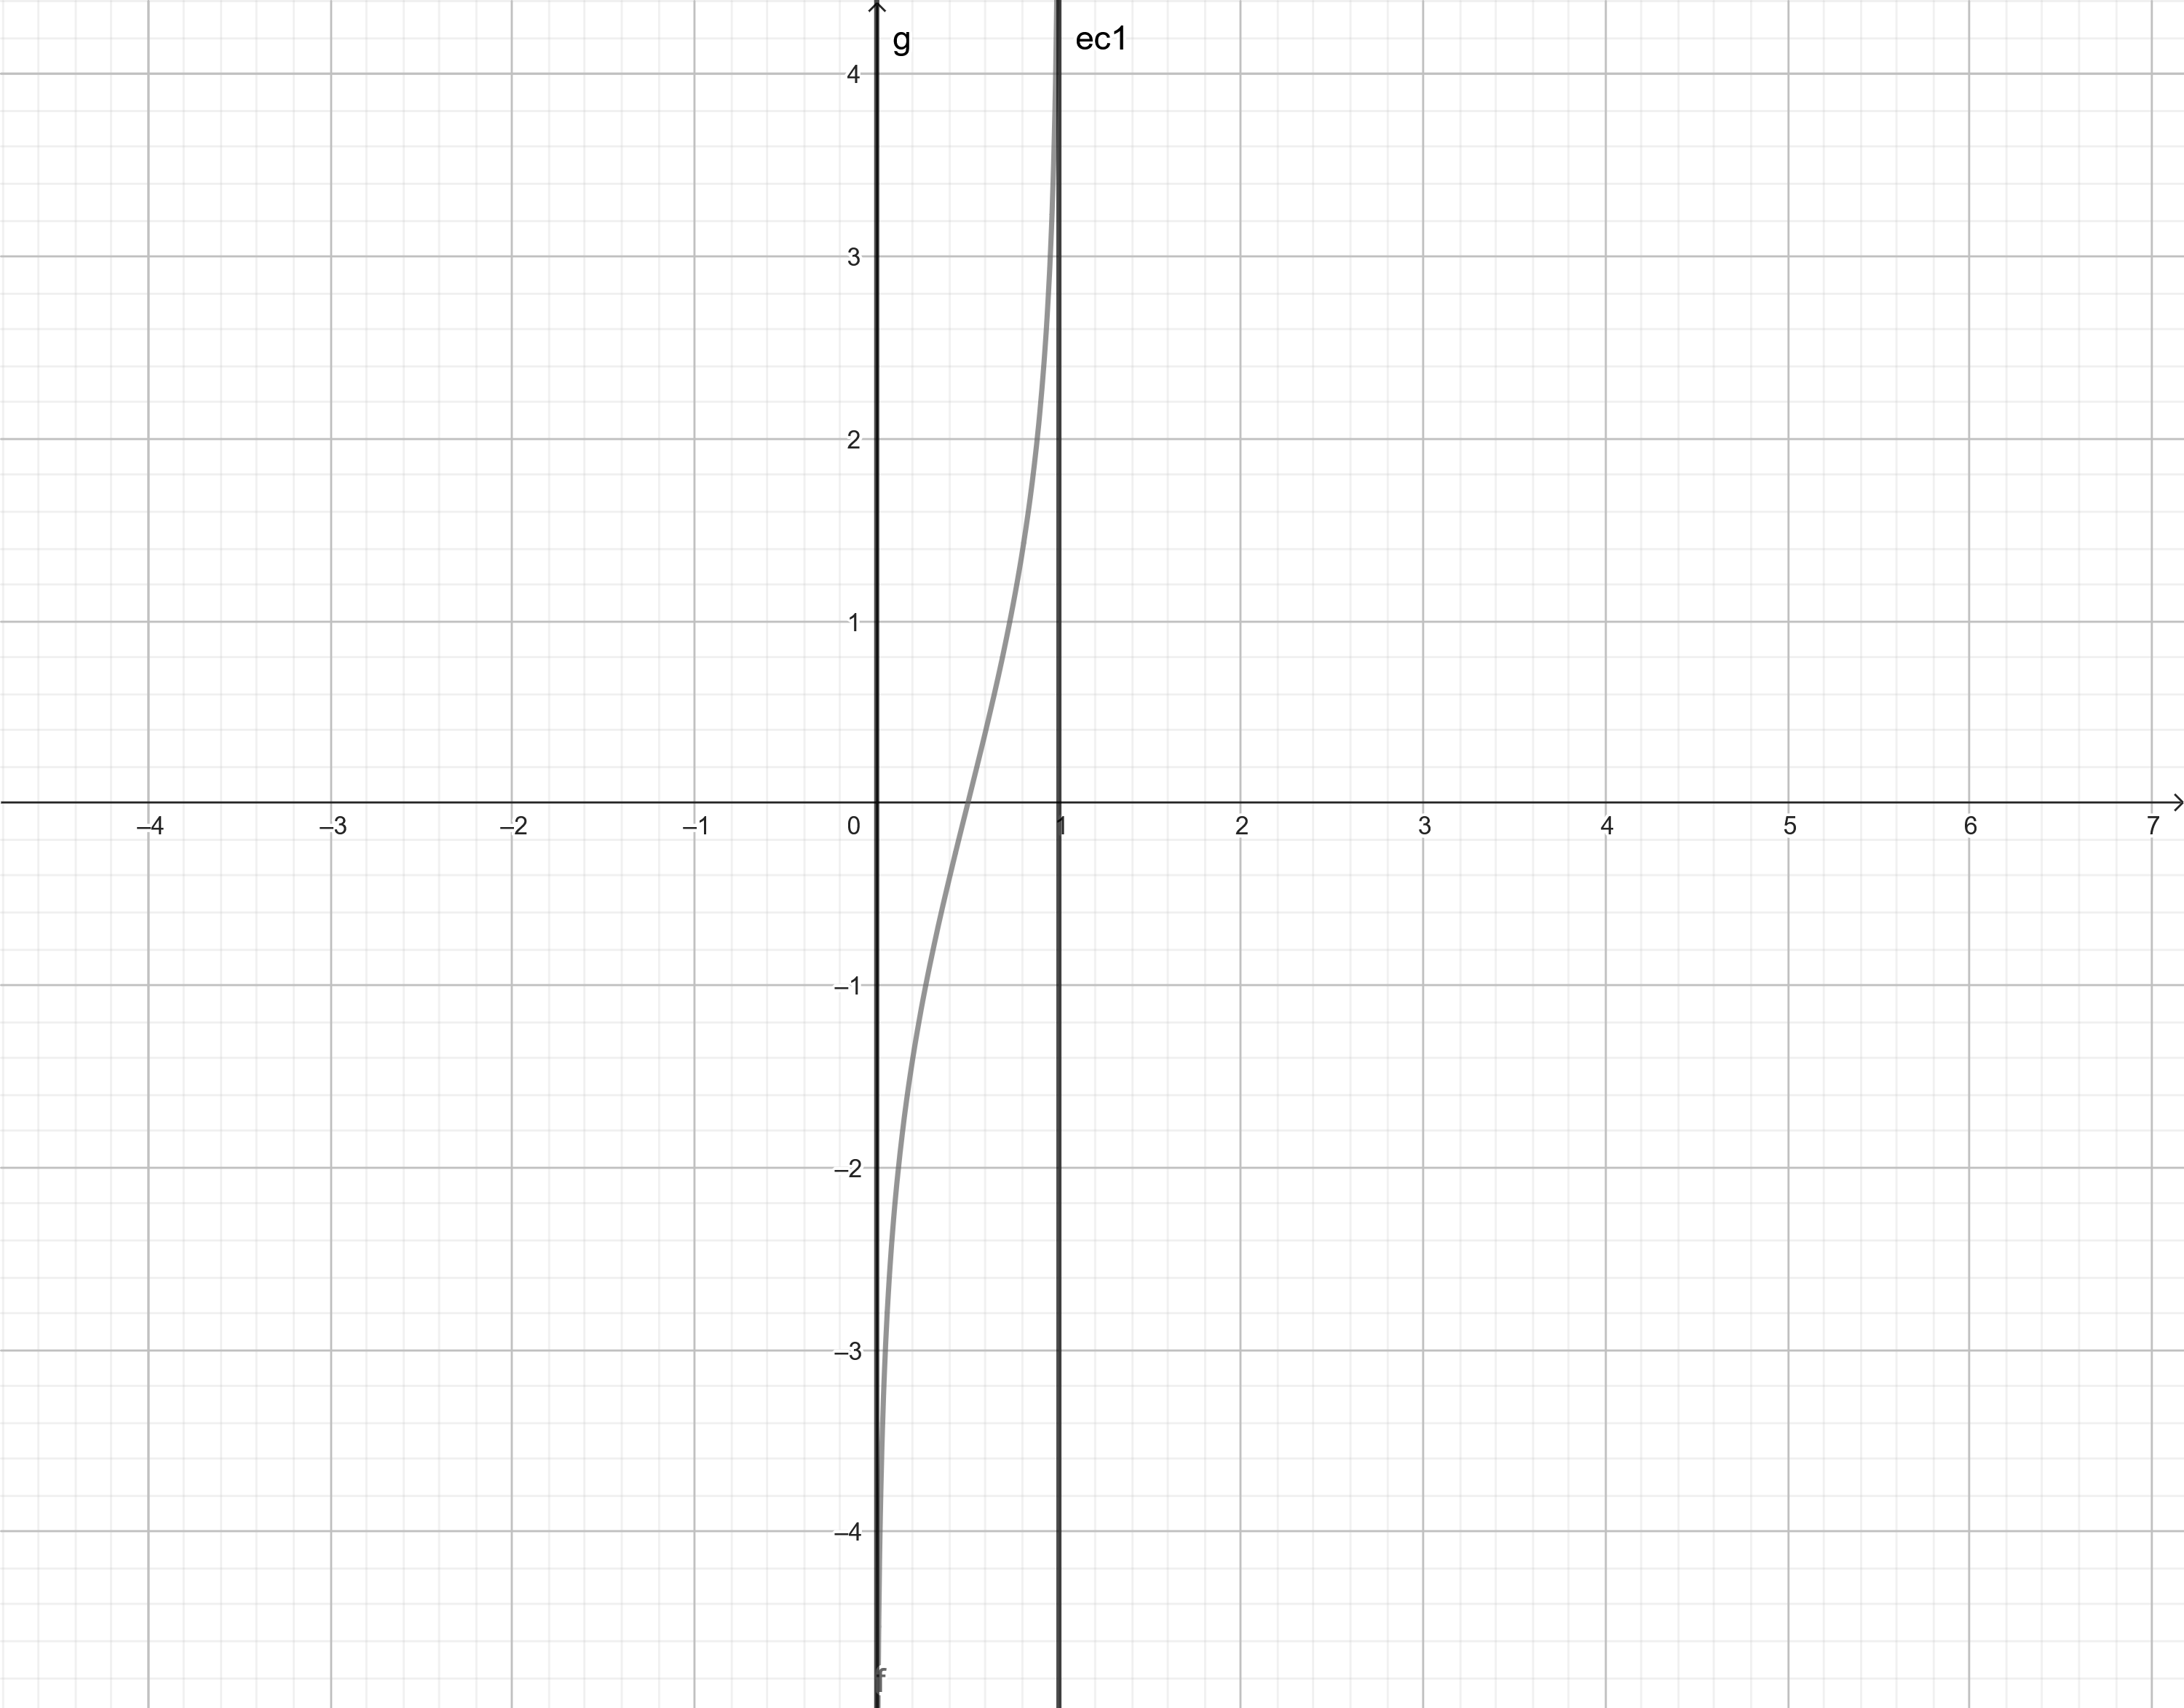
\includegraphics[width=0.5\linewidth]{Graficos/geogebra-export.png}
	\end{center}
	La imagen coincide con los números reales $\mathbb{R}$ por lo que contiene un conjunto abierto no trivial y por tanto el estadístico natural $\sum x_i$ es completo. 
}

Ahora veamos otro ejemplo en el que no se puede provocar la perteniencia a la familia exponencial: 

\ejemplo{
	Sea $X \sim U(\theta, 7\theta) \implies f_{\theta}(x) = \frac{1}{6\theta}\cdot I_{(\theta, 7\theta)}(x) \implies$
	$$f_{\theta}(\vec{x}) = \left(\frac{1}{6\theta}\right)^n \cdot I_{(\theta, 7\theta)}(x_{(1)}) \cdot I_{(\theta, 7\theta)}(x_{(n)})$$
	Entonces por el Teorema de Factorización de Fisher, tenemos que el estadístico $T(\vec{x}) = (x_{(1)}, x_{(n)})$ es suficiente.\\
	\begin{observación}
		Como la función indicadora depende de $\theta$, entonces la distribución no pertenece a la familia exponencial
	\end{observación}
	Recordemos además cuáles son las funciones de densidad de los máximos y lo mínimos (\underline{aunque en la práctica real hace falta demostrarlo siempre}): 
	$\begin{cases}
		f_{\theta}(x_{(n)}) = n(F_X(x))^{n-1} \cdot f_X(x) \\
		f_{\theta}(x_{(1)}) = n(1 - F_X(x))^{n-1} \cdot f_X(x)
	\end{cases} \implies$
	Saquemos primero la esperanza del máximo: \\
	$$E_{\theta}[x_{(n)}] = \int_{\theta}^{7\theta} x\cdot n\left(\frac{x - \theta}{6\theta}\right)^{n-1} \cdot \frac{1}{6\theta}dx =$$
	Para calcularla introduzcamos el cambio de variable, para usar la regla de la multipicación: $\begin{cases} x = u \\ dv = f_{\theta}(x_{(n)}) \end{cases} \implies$
	$$ = \left[x \cdot \left(\frac{x - \theta}{6\theta}\right)^n\right]^{7\theta}_{x = \theta} - \int_{\theta}^{7\theta} \left(\frac{x - \theta}{6\theta}\right)^{n} dx = 7\theta - \int_{y = 0}^{y = 1} y^n \cdot 6\theta dy = 7\theta - 6\theta \cdot \frac{1}{n+1} = \theta\frac{7n+1}{n+1}\theta$$
	Ahora, realicemoslo para el mínimo:\\
	$$E[x_{(1)}] = \int_{\theta}^{7\theta} x\cdot n\left(1 - \frac{x - \theta}{6\theta}\right)^{n-1} \cdot \frac{1}{6\theta}dx = \int^{7\theta}_{\theta} x\cdot n\left(\frac{7\theta - x}{6\theta}\right)^{n-1} \cdot \frac{1}{6\theta}dx =$$
	Al igual que antes introduzcamos un cambio de variable para calcularla: 
	$$ = \left[x \cdot \left(1 - \frac{x - \theta}{6\theta}\right)^n\right]^{7\theta}_{x = \theta} - \int_{\theta}^{7\theta} \left(\frac{7\theta - x}{6\theta}\right)^{n} dx = -\theta - \int_{1}^{0} y^n(-6\theta)dy =  -\theta - 6\theta\left[\frac{y^{n+1}}{n+1}\right]^{1}_{0} = -\theta - 6\theta\frac{1}{n+1}$$
	HAY QUE TERMINAR ESTE EJEMPLO
}


\begin{teorema}[Teorema de Basu]
	Si $T = T(X_1, \ldots, X_n)$ es un estadístico suficiente y completo y $U = U(X_1, \ldots, X_n)$ es un estadístico ancilario, entonces $T$ y $U$ son independientes
\end{teorema}

\begin{proof}
	Sea la muestra $(x_1, \ldots, x_n)$, un parámetro $\theta$ y sea un estadístico $T$ suficiente, entonces por definición tenemos que: 
	$$f(\vec{x} | T = t) \text{es indendiente de } \theta \implies$$
	$$f(U = u | T = t) = \sum_{\vec{x} : U(\vec{x}) = u} f(\vec{x} | T = t) \text{ es independiente de } \theta$$
	Aplicando las propiedades de los condicionales, tenemos que: 
	$$f_{\theta}(u) = f_{\theta}(t)f_{\theta}(u | t) \text{ pero como U es ancilario y T es completo, entonces:} \implies f(u) = f_{\theta}(t)f(u | t)$$

	Tomemos la función $h(t) = f(u | t) - f(u)$, entonces:
	$$E[h(T)] = E[f(u | T) - f(u)] = E[f(u | T)] - E[f(u)] = \int f(u | t)f(t)dt - \int f(u)f(t)dt = f(u) - f(u) = 0$$
	Entones como $T$ es completo, tenemos que $h(T) = 0$ c.s. $\implies f(u | t) = f(u) \implies$
	$$f(u | t) = \frac{f(u, t)}{f(t)} \iff f(t, u) = f(u)f(t) \implies U \text{ y } T \text{ son independientes}$$
\end{proof}

\ejemplo{
	Sea $X \sim U(0, \theta)$, veamos que $X_{(n)}$ y $\frac{X_{(1)}}{X_{(n)}}$ son independientes:\\
	$$ X \sim U(0, \theta) \implies f_{\theta}(x) = \frac{1}{\theta} \cdot I_{(0, \theta)}(x) \implies F_{X_{(n)}}(x) = P(X_{(n)} \leq x) = P(X_1 \leq x, \ldots, X_n \leq x) = $$ $$ = P(X_1 \leq x)\cdot \ldots \cdot P(X_n \leq x) = (F(x))^n = \left(\frac{x}{\theta}\right)^{n} \implies f_{\theta}(x) = n\left(\frac{x}{\theta}\right)^{n-1} \cdot \frac{1}{\theta} = \frac{n}{\theta^n}x^{n-1}$$
	Dado que por el Teorema de Factorización de Fisher, esta distribución es suficiente, consideraremos que $X_{(n)}$ es el estadístico suficiente y completo.\\
	Veamos ahora la función de densidad de $\frac{X_{(1)}}{X_{(n)}}$, para ello calculemos la función de densidad de $X_{(1)}$:
	$$F_{X_{(1)}}(x) = P(X_{(1)} \leq x) = 1 - P(X_{(1)} > x) = 1 - P(X_1 > x, \ldots, X_n > x) = $$ $$ = 1 - P(X_1 > x)\cdot \ldots \cdot P(X_n > x) = 1 - (1 - F(x))^n = 1 - \left(1 - \frac{x}{\theta}\right)^n \implies f_{\theta}(x) = n\left(1 - \frac{x}{\theta}\right)^{n-1} \cdot \frac{1}{\theta} = \frac{n}{\theta^n}(\theta - x)^{n-1}$$
}

\ejemplo{
	Sea una m.a.s. de tamaño $n$ de una población $X \sim N(\theta, \sigma)$ se tiene que: 
	$$\bar{X} \sim N(\mu, \frac{\sigma}{n}) \text{ ya que } \begin{cases} E[\bar{X}] = E\left[\frac{1}{n}\sum_{i = 1}^{n}X_i\right] = \frac{1}{n}\sum_{i = 1}^{n}E[X_i] = \frac{1}{n}n\theta = \theta \\ Var(\bar{X}) = Var\left(\frac{1}{n}\sum_{i = 1}^{n}X_i\right) = \frac{1}{n^2}\sum_{i = 1}^{n}Var(X_i) = \frac{1}{n^2}n\sigma = \frac{\sigma}{n} \end{cases}$$
	Y como se trata de una distribución perteneciente a la familia exponencial 2-paramétrica, entonces $\bar{X}$ es suficiente. Queda demostrar que sea completo, para ello, consideremos la función de densidad de $\bar{X}$:
	$$\bar{X} \sim N(\mu, \frac{\sigma}{n}) \implies f_{\theta}(x) = \sqrt{\frac{n}{2\pi\sigma}}e^{-\frac{n}{2\sigma}(x - \theta)^2}$$
	La completitud se da por definición. No obstante es una integral demasiado dificil de calcular, por lo que se puede deducir que $\bar{X}$ es completo. 
	Por el Teorema de Fisher sabemos que: 
	$$\frac{(n-1)S^2}{\sigma^2} \sim \chi^2(n-1) \implies S^2 \sim \frac{\sigma^2}{n-1}\chi^2(n-1) \implies S^2 \text{ es un estadístico ancilario} \implies$$
	Por el teorema de Basu, $\bar{X}$ y $S^2$ son independientes
}
    
    
\subsection{Principios de reducción de datos}

La idea es considerar la distribución de la probabilidad de la muestra, no como una función de $x = (x_1, \ldots, x_n)$, sino como una función del parámetro $\theta$ desconocido.
\begin{definición} [Función de verosimilitud]
	Dada la familia $\mathcal{P} = \{ f(\vec{x}|\theta) | \theta \in \Theta \}$ de distribuciones de probabilidad donde $f(\cdot|\theta)$ es una función de densidad o de masa y supuesto que se ha observado el valor muestral $\vec{x} = (x_1, ..., x_n)$ la función de $\theta$ definida mediante
	\[
	L(\theta|\vec{x}) = f(\vec{x}|\theta)
	\]
	se llama función de verosimilitud.
\end{definición}

\begin{definición} [Principio de verosimilitud]
	Sea $E = (\chi, \theta, \mathcal{P} = \{f(\vec{x}|\theta) : \theta \in \Theta\})$ un experimento aleatorio y $L_1(\theta | x)$ y $L_2(\theta | y)$ las funciones de verosimilitud de dos muestras $X = (x_1, \ldots, x_n)$ e $Y = (y_1, \ldots, y_m)$ respectivamente.\\
	Si existe una función $c(x, y)$ que no depende de $\theta$ tal que:
	$$L_1(\theta | x) = c(x, y)L_2(\theta | y) \ \forall \theta \in \Theta$$
	entonces se dice que ambas muestras suministran la misma evidencia estadística sobre el parámetro $\theta$, es decir, $Ev(E_1, \vec{x}) = Ev(E_2, \vec{y})$.
\end{definición}

\ejemplo{
	Sea un modelo $Binomial(n, \theta)$ la evidencia que se obtiene del mismo, sobre $\theta$, cuando se observan $t$ éxitos en $n$ repeticiones, es la misma que la obtenida por un modelo $Binomial negativo(t, \theta)$, siempre que se suponga que se han realizado $n$ repeticiones hasta obtener $t$ éxitos.\\
	$$ \text{En el primer caso tenemos que: } 
	f(t|\theta) = \binom{n}{t}\theta^t(1 - \theta)^{n-t} $$ $$\text{ y en el segundo caso: } g(\text{n repeticiones hasta obtener t éxitos} | \theta) = \binom{n-1}{t-1}\theta^t(1 - \theta)^{n-t}$$
	Por tanto, se puede aplicar el principio de verosimilitud, tomando la constante $c(t, n) = \frac{n}{t}$. Es decir, si para estimar la probabilidad con la que sale cara una moneda, se tira ésta $n$ veces,  y es $t$ el numero de cara s que se han presentado (modelo binomial), se obtiene la misma evidencia para $\theta$, que si se repite el experimento hasta observar $t$ caras y para ello ha habido que realizar $n$ repeticiones (modelo binomial negativo)
}
 

\begin{definición}[Principio de suficiencia]
	En un experimento $E = \left(\chi, \theta, \mathcal{P} = \{f(\vec{x}|\theta) : \theta \in \Theta\} \right)$, si $T = T(\vec{X})$ es un estadístico suficiente para $\theta$ y se tiene que $T(\vec{x}) = T(\vec{y})$, entonces las dos muetras $\vec{x}$ e $\vec{y}$ suministran la misma evidencia estadística, es decir, $Ev(E, \vec{x}) = Ev(E, \vec{y})$
\end{definición}

\ejemplo{
	En un experimento consistente en la repetición de $n$ pruebas de Bernoulli, la evidencia estadística que se obtiene de dos puntos muestrales con el mismo número de éxitos es la misma.
}

\begin{definición}[Principio de condicionalidad]
	El principio de condicionalidad dice que si un mecanismo aleatorio no depende del valor a determinar $\theta$, no proporciona evidencia sobre él. Es decir, si $T = T(\vec{X})$ es un estadístico suficiente para $\theta$ y $T(\vec{x}) = T(\vec{y})$, entonces las dos muestras $\vec{x}$ e $\vec{y}$ suministran la misma evidencia estadística, es decir, $Ev(E, \vec{x}) = Ev(E, \vec{y})$
\end{definición}

\ejemplo{
	Dados dos experimentos $E_1 = (\chi^n, f_1(\vec{x}|\theta))_{\theta \in \Theta \subset \mathbb{R}^{\ell}}$ y $E_2 = (\chi^m, f_2(\vec{y}|\theta))_{\theta \in \Theta \subset \mathbb{R}^{\ell}}$ y el lanzamiento de una moneda al aire representado por la v.a. $J$ tal que $P(J = 1) = P(J = 2) = \frac{1}{2}$, si $E = (\chi^n \cup \chi^m \times \{1, 2\}, f(\vec{x}, j|\theta))_{\theta \in \Theta \subset \mathbb{R}^{\ell}}$ es el experimento mixto representado por la v.a. $(Z, J)$ tal que $Z = \begin{cases} X & \text{ si } J = 1 \\ Y & \text{ si } J = 2 \end{cases}$, entonces $Ev(E, (\vec{x}, 1)) = Ev(E_1, \vec{x})$ y $Ev(E, (\vec{y}, 1)) = Ev(E_2, \vec{y})$
}
  
\begin{teorema}[Teorema de Birnbaum]
	El principio de verosimilitud es equivalente a los principios de suficiencia y condicionalidad.
\end{teorema}  

\subsection{Ejercicios}
\begin{problem}{2.1}
	Sea $X$ muestra de una población $N(0, \sigma)$, ¿Es $T(X) = |X|$ un estadístico suficiente?
\end{problem}
\begin{sol}
	Recordemos la definición de estadístico suficiente por definición: Dado un estadístico $T$ en este caso $T(X) = |X|$ y una muestra $\vec{x}$ se dice que $T$ es suficiente si $f_{\theta}(\vec{X} = \vec{x} | T = t)$ \\
	Empecemos definiendo la distribución que sigue el estadístico $T$: 
	$$P(|X| \leq a) = P(-a \leq X \leq a) = P(X \leq a) - P(X \leq -a) = F(a) - F(-a) = 2F(a) = 2\int_{0}^{a}f_{X}(x)dx$$
	$$\implies f_{|X|}(x) = 2f_{X}(x) = 2\cdot \frac{1}{\sqrt{2\pi}\sigma}e^{-\frac{(x - \mu)^2}{2\sigma^2}} \implies \text{ Si } X \sim N(0, \sigma) \implies f_{|X|}(x) = \frac{\sqrt{2}}{\sigma\sqrt{\pi}}\cdot e^{-\frac{x^2}{2\sigma^2}}$$
	Entonces veamos el cociente de las dos funciones de densidad:
	$$P(X = x | T = t) = \frac{f_{\sigma}(x)}{f_{\sigma}(t)} = \frac{\frac{1}{\sigma\sqrt{2\pi}}\cdot e^{-\frac{x^2}{2\sigma^2}}}{\frac{\sqrt{2}}{\sigma\sqrt{\pi}} \cdot e^{-\frac{x^2}{2\sigma^2}}} = \frac{1}{2}$$
	Lo cual no depende del parámetro $\sigma$ y por tanto por definición, el estadístico es suficiente. 
\end{sol}

\begin{problem}{2.2}
	Encuentra un estadístico suficiente para una m.a.s. de tamaño $n$ de cada una de las siguientes poblaciones: 
	\begin{enumerate}
		\item Beta($\alpha, \beta$) : $\alpha > 0, \beta > 0$
		\item Gamma($a, p$) : $a > 0, p > 0$
		\item $p_{N_1 N_2}(x) = \frac{1}{N_2 - N_1} \cdot I_{N_1 + 1, N_1 +2 \ldots, N_2}(x)$ : $N_1 < N_2$
		\item $f_{\theta}(x) = e^{-x + \theta}\cdot I_{\theta, \infty}(x)$
		\item $f_{\mu, \sigma}(x) = \frac{1}{x\sigma\sqrt{2\pi}}e^{-\frac{1}{2\sigma^2}(\ln(x - \mu))^2}\cdot I_{0, \infty}$
		\item $p_{\theta, p}(x) = (1 - p)p^{x - \theta} \cdot I_{\theta, \theta + 1, \ldots }(x)$
	\end{enumerate}
\end{problem}
\begin{sol}
	\begin{enumerate}
		%Primer caso%
		\item Sea $X \sim Beta(\alpha, \beta) \implies$ $$f_{\alpha, \beta}(x) = \frac{x^{\alpha -1}(1 - x)^{\beta - 1}}{B(\alpha, \beta)} \implies f_{\alpha, \beta}(x_1, \ldots, x_n)(x) = \prod_{i = 1}^{n}f_{\alpha, \beta}(x_i) = \frac{(\prod_{i = 1}^{n}x_i)^{\alpha -1}(\prod_{i = 1}^{n}(1-x))^{\beta -1}}{B(\alpha, \beta)^n}$$
		Entonces por el Teorema de Factorización de Fisher, tenemos que $$f_{\theta}(x) = h(x) \cdot g_{\theta}(T(x)) \implies T(\vec{x}) = (\prod_{i = 1}^{n}x_i, \prod_{i = 1}^{n}(1 - x_i))$$
		%Segundo caso%
		\item Sea $X \sim Gamma(\alpha, \beta) \implies$ $$f_{\alpha, \beta}(x) = \frac{\beta^{\alpha}}{\Gamma(\alpha)}x^{\alpha-1} \cdot e^{-x\beta} \implies f_{\alpha, \beta}(x_1, \ldots, x_n) = \prod_{i = 1}^{n}f_{\alpha, \beta}(x_i) = \frac{\beta^{n\alpha}}{\Gamma(\alpha)}(\prod_{i = 1}^{n}x_i)^{\alpha-1} \cdot e^{-\beta \sum_{i = 1}^{n}x_i}$$
		Entonces por el Teorema de Factorización de Fisher: $$f_{\theta} = h(x) \cdot g_{\theta}(T(x)) \implies T(\vec{x}) = (T_1(\vec{x}), T_2(\vec{x})) = (\sum_{i = 1}^{n}x_i, \prod_{i = 1}^{n}x_i)$$
		%Tercer caso%
		\item Sea $X \sim \text{Uniforme Discreta}(N_1 , N_2) \implies$
		$$ f_{(N_1, N_2)}(x) = \frac{1}{N_2 - N_1} \cdot I_{N_1 + 1, N_1 +2 \ldots, N_2}(x) \implies f_{(N_1, N_2)}(x_1, \ldots, x_n) = \prod_{i = 1}^{n}f_{(N_1, N_2)}(x_i) =$$ $$ = \frac{1}{(N_2 - N_1)^n} \cdot I_{\{N_1 + 1, N_1 +2, \ldots, +\infty\}}(x_{(1)}) \cdot I_{\{-\infty, \ldots, N_2 - 1, N_2\}}(x_{(n)})$$
		Por el Teorema de Factorización de Fisher, tenemos que: 
		$$f_{\theta}(x) = h(x) \cdot g_{\theta}(T(x)) \implies T(\vec{x}) = (x_{(1)}, x_{(n)})$$
		%Cuarto caso%
		\item Sea una variable aleatoria con función de densidad $f_{\theta}(x) = e^{-x + \theta}\cdot I_{\theta, \infty}(x) \implies$
		$$ f_{\theta}(x_1, \ldots, x_n) = \prod_{i = 1}^{n}f_{\theta}(x_i) = \prod_{i = 1}^{n}e^{-x_i + \theta}\cdot I_{\theta, \infty}(x_i) = e^{-\sum_{i = 1}^{n}x_i + n\theta}\cdot I_{\theta, \infty}(x_{(1)})$$
		Por el Teorema de Factorización de Fisher, tenemos que:
		$$f_{\theta}(x) = h(x) \cdot g_{\theta}(T(x)) \implies T(\vec{x}) = (x_{(1)})$$
		%Quinto caso%
		\item Sea una varible aleatoria $X$ cuya función de densidad es: 
		$$f_{(\mu, \sigma)}(x) = \frac{1}{x\sigma\sqrt{2\pi}}\cdot e^{-\frac{1}{2\sigma^2}(ln(x) - \mu)^2}\cdot I_{0, \infty}(x) \implies f_{(\mu, \sigma)}(\vec{x}) = \prod_{i = 1}^{n}\frac{1}{x_i} \left(\frac{1}{\sigma\sqrt{2\pi}}\right)^n \cdot e^{-\frac{1}{2\sigma}\sum_{i = 1}^{n}(\ln(x_i) - \mu)^2}$$
		Desarrollando el cuadrado: $(ln(x_i) - \mu)^2 = ln^2(x_i) - 2\mu ln(x_i) + \mu^2$ y conociendo que la forma general de las funciones de densidad de las familias exponenciales 2-paramétricas es: 
		$$f_{(\mu, \sigma)}(x) = c(\mu, \sigma) \cdot h(x) \cdot e^{q_1(\mu, \sigma)T_1(x) + q_2(\mu, \sigma)T_2(x)} \implies f_{(\mu, \sigma)}(\vec{x}) = c(\mu, \sigma)^n \cdot h(\vec{x}) \cdot e^{q_1(\mu, \sigma)\sum T_1(x_i) + q_2(\mu, \sigma)\sum T_2(x_i)}$$
		Podemos ver que $T_1(\vec{x}) = \sum_{i = 1}^{n}ln(x_i)$ y $T_2(\vec{x}) = \sum_{i = 1}^{n}ln^2(x_i)$
		\begin{observación}
			Esta distribución en particular se la conoce como log-normal o distribucion de Tinaut y surge de tomar una distribución normal $N(\mu, \sigma)$ y aplicarle la función logarítmica, es decir: $Y = ln(X) \sim N(\mu, \sigma)$
		\end{observación}
		%Sexto caso%
		\item Sea una variable aleatoria $X$ cuya función de densidad es: 
		$$f_{(\theta, p)}(x) = (1 - p)p^{x - \theta} \cdot I_{\theta, \theta + 1, \ldots }(x) \implies f_{(\theta, p)}(\vec{x}) = (1-p)^n \cdot p^{\sum_{i = 1}^{n}x_i - n\theta} \cdot I_{\theta, \theta + 1, \ldots }(x_{(1)})$$
		Entonces por el Teorema de Factorización de Fisher, tenemos que: 
		$$ f_{\theta}(x) = h(x) \cdot g_{\theta}(T(x)) \implies T(\vec{x}) = (\sum_{i = 1}^{n}x_i, x_{(1)})$$
	\end{enumerate}
\end{sol}
\begin{problem}{2.3}
	Sea una m.a.s. de tamaño $n$ de una población con función de distribución $X \sim Uniforme(\theta, 4\theta)$ pruébese que $(X_{(1)}, X_{(n)})$ es un estadístico suficiente para $\theta$ pero no es completo. 
\end{problem}

\begin{sol}
	$$X \sim U(\theta, 4\theta) \implies f_{\theta}(x) = \frac{1}{3\theta} \cdot I_{(\theta, 4\theta)}(x) \implies f_{\theta}(x_1, \ldots, x_n) = \frac{1}{(3\theta)^n} \cdot I_{(\theta, 4\theta)}(x_{(1)}) \cdot I_{(\theta, 4\theta)}(x_{(n)})$$
	Entonces, por el Teorema de Factorización de Fisher, tenemos que: $f_{\theta}(x) = h(x) \cdot g_{\theta}(T(x)) \implies T(\vec{x}) = (x_{(1)}, x_{(n)})$ 
	Ahora veamos que el estadístico no es completo: 
	Para ello tenemos que sacar cuales son las distribuciones del mínimo y el máximo:
	\begin{enumerate}
		%El máximo%
		\item $$f_{\theta}(x_{(n)}) = n(F(x))^{n-1} \cdot f_{\theta}(x_{(n)}) = n\left(\frac{x - \theta}{3\theta}\right)^{n-1} \cdot \frac{1}{3\theta} = \frac{n}{3\theta^n}(x - \theta)^{n-1} \implies$$
		$$E[T_1] = \int_{\theta}^{4\theta}x \cdot n\left(\frac{x - \theta}{3\theta}\right)^{n-1} \cdot \frac{1}{3\theta}dx = \left[x\cdot \left(\frac{x - \theta}{3\theta}\right)^n\right]_{\theta}^{4\theta} - \int_{\theta}^{4\theta} \left(\frac{x - \theta}{3\theta}\right)^n dx = 4\theta - 3\theta\int_{0}^{1}y^n dy = $$ $$ = 4\theta - 3\theta\frac{1}{n+1} = \theta\frac{4n + 1}{n+1}$$
		%El minimo%
		\item $$f_{\theta}(x_{(1)}) = n(1 - F(x))^{n-1} \cdot f_{\theta}(x) = n\left(1 - \frac{x - \theta}{3\theta}\right)^{n-1} \cdot \frac{1}{3\theta} = \frac{n}{3\theta^n}(4\theta - x)^{n-1} \implies$$
		$$E[T_2] = \int_{\theta}^{4\theta} x \cdot n\left(1 - \frac{x - \theta}{3\theta}\right)^{n-1} \cdot \frac{1}{3\theta}dx = \left[x\cdot -\left(1 - \frac{x - \theta}{3\theta}\right)^n\right]_{\theta}^{4\theta} - \int_{\theta}^{4\theta} \left(\frac{4\theta - x}{3\theta}\right)^n dx = $$ $$ = \theta - 3\theta\int_{0}^{1}y^n dy = \theta - 3\theta\frac{1}{n+1} = \theta\frac{4n + 1}{n+1}$$
	\end{enumerate} 
\end{sol}

\begin{problem}{2.4}
	Sea una m.a.s. de una población que sigue una variable aleatoria $X$ con función de densidad: 
	$$f_{\theta}(x) = e^{-(x - \theta)} \cdot I_{(\theta, +\infty)}(x)$$
	\begin{enumerate}
		\item Pruébese que $T(\vec{X}) = X_{(1)}$ es un estadístico suficiente y completo para $\theta$
		\item Mediante el Teorema de Basu, pruébese que $X_{(1)}$ y $S^2$ son independientes. 
	\end{enumerate} 
\end{problem}
\begin{sol}
	Antes de comenzar con la resolución del problema, calculemos la función de densidad de la muestra: 
	$$f_{\theta}(\vec{x}) = e^{-\sum_{i = 1}^{n}x_i + n\theta} \cdot I_{\theta, +\infty}(x_{(1)})$$
	\begin{enumerate}
		\item Para demostrar la suficiencia usaremos el Teorema de Factorización de Fisher con: $f_{\theta}(\vec{x}) = h(\vec{x}) \cdot g_{\theta}(T(\vec{x})) = e^{-\sum_{i = 1}^{n}x_i + n\theta} \cdot I_{\theta, +\infty}(x_{(1)})$ y $T(\vec{x}) = (x_{(1)}, \sum x_i)$\\
		Ahora veamos la completitud: Sea una función real $g(x)$ que cumpla que: $$E[g(x_{(1)})] = 0 = \int_{\theta}^{+\infty}g(x)f_{\theta}(x)dx = \int_{\theta}^{+\infty}g(x)e^{-x + \theta}dx$$
		Si tomamos cómo función $H(x) = \int_{t > 0}^{+\infty} e^{-y}$ sabemos que dicha función es positiva en todo su dominio, por lo que la únia manera de que la integral anterior sea nula es que $g(x) = 0$ c.s. $\implies$ el estadístico es completo.
		\item El Teorema de Basu, nos dice que si $T$ es un estadístico suficiente y completo y $U$ es un estadístico ancilario, entonces $T$ y $U$ son independientes. En este caso, sabemos que $X_{(1)}$ es completo y suficiente, y por el Teorema de Basu, sabemos que $X_{(1)}$ y $S^2$ son independientes.
		Entonces debemos comprobar que $S^2$ es ancilario: 
		$$ f_{\theta} = e^{-(x - \theta)} \implies X \sim Exponencial(1) + \theta \implies S^2 = \frac{1}{n-1}\sum_{i = 1}^{n}(X_i - \bar{X})^2 =$$  $$= \frac{1}{n-1}\sum_{i = 1}^{n} (X_i - \theta + \theta - \bar{X})^2 = \frac{1}{n-1}\sum_{i = 1}^{n} (X_i - \theta - (\bar{X} - \theta)^2) = \frac{1}{n-1}\sum_{i = 1}^{n} (Z_i - \bar{Z})^2 \implies $$ $$\implies Z \sim Exponencial(1) \text{ no depende de } \theta \implies S^2 \text{ es ancilario}$$
		Por tanto por el Teorema de Basu, ambos estadísticos son independientes.
	\end{enumerate}
\end{sol}
\begin{problem}{2.5}
	Sea una población que sigue una variable aleatoria $X$ con fucniones de masa: 
	$$P_{\theta}(X = -1) = \theta \quad P_{\theta}(X = x) = (1 - \theta)^2\cdot\theta^x\cdot I_{0 \cup \mathbb{N}}(x)$$
	Con $\theta \in (0, 1)$	y el tamaño de la muestra $n = 1$ ¿El estadístico $X$ es completo?
\end{problem}
\begin{sol}
	$$E[X] = \sum_{i = 0}^{+\infty} P(X = i) \cdot i = -1\cdot P(X = -1) + \sum_{i = 1}^{+\infty} P_{\theta}(X = i) \cdot i = -1 \cdot \theta + \sum_{i = 1}^{n} (1 - \theta)^2 \cdot i\theta^{i} = $$ $$ = -\theta + (1 - \theta) \sum_{i = 1}^{n}i\theta^{i} = -\theta + (1 - \theta)t'(x) \text{ donde } t(x) = \sum_{i = 1}^{\infty}\theta^i = \frac{\theta}{1 - \theta} \implies t'(x) = \frac{1}{(1-\theta)^2}$$ $$\implies E[X] = -\theta + (1 - \theta)^2\theta(\frac{1}{(1 - \theta)^2}) = -\theta + \theta = 0$$
	Entonces, como $E[X] = 0$, $X$ no es completo.
\end{sol}
\begin{problem}{2.6}
	Sea m.a.s. de tamaño $n$ de una población $N(\alpha\sigma, \sigma) : \alpha \in \mathbb{R}$ veamos si el estadístico $T(\vec{X}) = (\sum_{i = 1}^{n}X_i, \sum_{i = 1}^{n}X_i^2)$ es suficiente y completo para $\sigma$.
\end{problem}
\begin{sol}
	$$X \sim N(\alpha\sigma, \sigma) \implies f_{\sigma}(x) = \frac{1}{\sigma\sqrt{2\pi}}e^{-\frac{(x - \alpha\sigma)^2}{2\sigma^2}} \implies f_{\sigma}(\vec{x}) = \prod_{i = 1}^{n}f_{\sigma}(x_i) = \left(\frac{1}{\sigma\sqrt{2\pi}}\right)^n \cdot e^{-\frac{1}{2\sigma^2}\sum_{i = 1}^{n}(x_i - \alpha\sigma)^2}$$
	Entonces descomoponiendo: $(x_i - \alpha\sigma)^2 = x_i^2 + \alpha^2\sigma^2 - 2\alpha\sigma x_i \implies$
	$$f_{\sigma}(\vec{x}) = \left(\frac{1}{\sigma\sqrt{2\pi}}\right)^n \cdot e^{-\frac{1}{2\sigma^2}\sum_{i = 1}^{n}x_i^2 + \frac{\alpha}{\sigma}\sum_{i = 1}^{n}x_i  - \frac{n\alpha^2}{2}} $$
	Entonces por el Teorema de Factorización de Fisher, tenemos que el estadístico $T(\vec{x}) = (\sum_{i = 1}^{n}x_i, \sum_{i = 1}^{n}x_i^2)$ es suficiente. \\
	Ahora veamos si es completo:\\
	$$E\left[\sum_{i = 1}^{n}X_i\right] = n\alpha\sigma \quad E\left[\sum_{i = 1}^{n}X_i^2\right] = n\sigma^2 + n\alpha^2\sigma^2 = (1 + n\alpha^2)n\sigma^2$$
	Pero la función 
	$$g(\vec{T}) = \frac{1}{1 + n\alpha^2}\left(\sum_{i = 1}^{n}X_i\right)^2 - \frac{1}{1 + \alpha^2}\sum_{i = 1}^{n}X_i^2 \implies E[g(\vec{T})] = 0$$
	Pero la función no es nula en casi todo punto, por lo que no es completo. 
\end{sol}
\begin{problem}{2.7}
	Sea una población con variable aleatoria $X \sim Uniforme(\theta, \theta + 1)$ y una m.a.s. de tamaño $n$ de dicha población. Entonces, 
	\begin{enumerate}
		\item Encuentra un estadístico suficiente para $\theta$
		\item Comprueba si el recorrido muestral $R = X_{(n)} - X_{(1)}$ es un estadístico ancilario
		\item Si la función de de distribución sufriera un desplazamiento de $F_{\theta}(x) = F(x - \theta)$ Comprueba si se conserva la propiedad del apartado anterior
	\end{enumerate}
\end{problem}
\begin{sol}1
	\begin{enumerate}
		\item $X \sim Uniforme(\theta, \theta + 1) \implies f_{\theta}(x) = \frac{1}{\theta + 1 - \theta} \cdot I_{(\theta, \theta + 1)} = 1 \cdot I_{(\theta, \theta +1)}(x) \implies f_{\theta}(\vec{x}) = I_{(\theta, \theta + 1)}(x{(1)})\cdot I_{(\theta, \theta +1)}(x_{(n)})  \implies$ por el Teorema de Factorización de Fisher, el estadístico $T(\vec{x}) = (x_{(1)}, x_{(n)})$ es suficiente.
		\item Calculemos las funciones de distribución del máximo y el mínimo: 
		\begin{itemize}
			\item $$f_{\theta}(x_{(n)}) = n(F(x))^{n-1} \cdot f_{\theta}(x_{(n)}) = n\left(\frac{x - \theta}{1}\right)^{n-1} \cdot 1 = n(x - \theta)^{n-1}$$ 
			\item $$f_{\theta}(x_{(1)}) = n(1 - F(x))^{n-1} \cdot f_{\theta}(x_{(1)}) = n\left(1 - \frac{x - \theta}{1}\right)^{n-1} \cdot 1 = n(\theta + 1 - x)^{n-1} \implies$$
			Cuando intentamos calcular la probabilidad $P(R \leq r)$ estamos calculando la probabilidad de que el máximo y el mínimo estén a menos de una distancia $r$, entonces: 
			$$P(R \leq r) = \int_{\theta}^{\theta +1} f_{X_{(n)}}(x) \cdot P(x - X_{(1)} \leq r)dx$$
			Intuitivamente, esta expresión nos dice la probabilidad de que un punto $x$ del intervalo sea el máximo por la probabilidad de que la distancia de ese número menos el mínimo esté a una distancia menor que $r \implies$
			$$P(R \leq r) = \int_{\theta}^{\theta +1} n(x - \theta)^{n-1} \cdot P(x - X_{(1)} \leq r)dx = \int_{\theta}^{\theta +1} n(x - \theta)^{n-1} \cdot P(X_{(1)} \geq x - r)dx =$$ $$ = \int_{\theta}^{\theta +1} n(x - \theta)^{n-1} \cdot (1 - P(X_{(1)} \leq x - r))dx = \int_{\theta}^{\theta +1} n(x - \theta)^{n-1} \cdot (\theta + 1 - x + r)^n dx = $$ $$ = \int_{0}^{1} n y^{n-1}\cdot (1 + r - y)^{n}dy$$
			Donde $y = x - \theta$ y $r = r - \theta$ y dado que es una expresión que no depende de $\theta$ llegamos a que el estadístico es ancilario. 
			\item Si tenemos en cuenta el caso general del desplazamiento en una distribución uniforme: $$F_{\theta}(x) = F(x - \theta)  \implies P:{\theta}(r) = P(X_{(n)} - X_{(1)} \leq r) \implies$$
			Si hacemos el cambio de varibale $Z_i = X_i - \theta$ obtenemos que $Z_{(n)} - Z_{(1)} = X_{(n)} - X_{(1)}$ y por tanto, el recorrido muestral sigue siendo un estadístico ancilario.  
		\end{itemize}
	\end{enumerate}
\end{sol}
\begin{problem}{2.8}
	Dada una m.a.s. de tamaño $n$ de una población donde se sigue la siguiente función de densidad: 
	$$f_{\theta}(x) = \frac{2x}{\theta^2}\cdot I_{(0, \theta)}(x)$$
	Entonces: 
	\begin{enumerate}
		\item Comprueba si $T(\vec{X}) = (X_{(n)}, \prod_{i = 1}^{n}X_i)$ es suficiente para $\theta$ y si además es minimal. 
		\item Comprueba también si $T_2(\vec{x}) = X_{(n)}$ es un estadístico completo. 
	\end{enumerate}
\end{problem}
\begin{sol}
	\begin{enumerate}
		\item $$f_{\theta}(x) = \frac{2x}{\theta^2} \cdot I_{(0, \theta)}(x) \implies f_{\theta}(\vec{x}) = \prod_{i = 1}^{n}f_{\theta}(x_i) = \frac{2^n}{\theta^{2n}} \cdot \prod_{i = 1}^{n}x_i \cdot I_{(0, \theta)}(x_{(n)})$$
		Entonces por el Teorema de Factorización de Fisher, el estadístico $T(\vec{x}) = (X_{(n)}, \prod_{i = 1}^{n}X_i)$ es suficiente. Para comprobar si es minimal, veamos que: \\
		Dadas dos muestras $\vec{x}$ y $\vec{y} \implies$ $$\frac{f_{\theta}(\vec{x})}{f_{\theta}(\vec{y})} = \frac{\frac{2^n}{\theta^{2n}} \cdot \prod_{i = 1}^{n}x_i \cdot I_{(0, \theta)}(x_{(n)})}{\frac{2^n}{\theta^{2n}} \cdot \prod_{i = 1}^{n}y_i \cdot I_{(0, \theta)}(y_{(n)})} = \frac{\prod_{i = 1}^{n}x_i \cdot I_{(0, \theta)}(x_{(n)})}{\prod_{i = 1}^{n}y_i \cdot I_{(0, \theta)}(y_{(n)})}$$
		Entonces, el cociente no depende de $\theta \iff T(\vec{x}) = T(\vec{y})$ por lo que el estadístico es minimal.
		\item Comprobemos que el estadístico $T_2(\vec{x}) = X_{(n)}$ es completo: \\
		Cómo es un máximo la función de densidad sigue una fórmula: 
		$$f_{X_{(n)}} = n(F(x))^{n-1} \cdot f_{X}(x) = n\left(\frac{x^2}{\theta^2}\right)^{n-1} \cdot \frac{2x}{\theta^2} = 2n\left(\frac{x^{2n-1}}{\theta^{2n}}\right)$$
		Entonces, para una función real $g(x)$ queremos ver si que $E[g(X_{(n)})] = 0$ implica que $g(x) = 0$ c.s.\\
		$$E[g(X_{(n)})] = \int_{0}^{\theta}g(x)2n\left(\frac{x^{2n-1}}{\theta^{2n}}\right)dx = \frac{2n}{\theta^{2n}}\int_{0}^{\theta}g(x) \cdot x^{2n-1}dx = 0 \implies$$
		Aplicando la Regla de Leibniz para derivadas de integrales: 
		$$\frac{d}{d\theta}\int_{a(\theta)}^{b(\theta)} f(x, \theta)dx = f(b(\theta), \theta) \cdot \frac{d}{d\theta}(b(\theta)) - f(a(\theta), \theta) \cdot \frac{d}{d\theta}(a(\theta)) + \int_{a(\theta)}^{b(\theta)} \frac{\partial}{\partial \theta}f(\theta, x) dx$$
		En nuestro caso, podemos sustituir usando: 
		\begin{itemize}
			\item $f(x, \theta) = g(x)\cdot x^{2n-1}$
			\item $b(\theta) = \theta$
			\item $a(\theta) = 0$
		\end{itemize}
		Entones tenemos que:
		$$\frac{d}{d\theta}\int_{0}^{\theta}g(x) \cdot x^{2n-1}dx = g(\theta)\cdot \theta^{2n-1} - g(0)\cdot 0^{2n-1} + \int_{0}^{\theta} \frac{\partial}{\partial \theta}(g(x) \cdot x^{2n-1})dx = $$ $$ = g(\theta)\cdot \theta^{2n-1} = 0 \implies g(\theta) = 0 \implies g(x) = 0 \text{ c.s.}$$
		Entones el estadístico $T_2(\vec{x}) = X_{(n)}$ es completo.
	\end{enumerate}
\end{sol}
\newpage
\end{comment}

\section{Estimación Puntual Paramétrica}

\begin{definición}[Estimador]
Sea $(\Omega, \mathcal{A}, \mathcal{P})$ el espacio probabilístico asociado a un experimento aleatorio $\mathcal{E}$, una variable aleatoria observable $X: \Omega \longrightarrow \mathbb{R}$ y su modelo estadístico asociado $\left(\chi, \mathcal{B}, F_{\theta}\right)_{\theta \in \Theta \subset \mathbb{R}^{\ell}}, \mathcal{B}=\mathcal{B}(\mathbb{R})$, y $\left(X_{1}, \cdots X_{n}\right)$ m.a.s. $(n) \sim X$
\\Un estimador del parámetro $\theta$ es un estadístico $T=T\left(X_{1}, \cdots X_{n}\right): \chi^{n} \longrightarrow \Theta$ que se utiliza para determinar el valor desconocido $\theta$
\end{definición}

\begin{definición}[Estimador centrado o insesgado]
Dado un estimador $T = T(X_1, \ldots X_n): \chi^{n} \to \Theta$ se dice que es centrado para $h(\theta)$ cuando $E_{\theta}[T] = h(\theta)$. \\
Se dice asintóticamente insesgado o centrado cuando $\lim_{n \to \infty}E_{\theta}[T] = h(\theta)$
\end{definición}

\ejemplo{
  Para cualquier población que tenga media, la media muestral \(\overline{X}\) es un estimador centrado de \(h(\theta) = E[X]\), puesto que se cumple:
  \[
    E_\theta \left[ \overline{X} \right] = E[X]
  \]

  Además, se tiene que \(E[a_k] = \alpha_k\), lo que implica que el momento
  muestral de orden \(k\) respecto al origen es un estimador centrado del momento
  poblacional de orden \(k\) respecto al origen de la población. En general, no
  es cierto un resultado análogo para momentos centrales. }

\begin{definición}[Sesgo]
Se llama sesgo de un estimador a la diferencia $b(T, \theta) = E_{\theta}[T] - \theta$
\end{definición}

\ejemplo{
Veamos que el estadístico $T = (\bar{X}, S^2)$ es un estimador centrado de $\theta = (\mu, \sigma^2):$\\
$$E[\bar{X}] = E\left[\frac{1}{n}\sum_{i  = 1}^{n} X_i \right] = \frac{1}{n} \sum_{i = 1}^{n}E[X_i] = \frac{1}{n} \sum_{i = 1}^{n} \mu = \mu$$
$$E[S^2] = E\left[\frac{1}{n-1}\sum_{i  = 1}^{n} (X_i - \bar{X})^2 \right] = \frac{1}{n-1} \sum_{i = 1}^{n}E[(X_i - \bar{X})^2] = \frac{1}{n-1} \sum_{i = 1}^{n} \sigma^2 = \sigma^2$$
}

\ejemplo{
Demuestra que el estadístico $\sigma_n^2 = b_2 = \frac{1}{n} \sum_{i = 1}^{n}(X_i - \bar{X})^2$ es un estimador centrado de $h(\theta) = \frac{n-1}{n}\sigma^2$ y $b(\sigma_n^2, \sigma^2) = -\frac{\sigma^2}{n}$
$$E[\sigma_n^2] = E\left[\frac{1}{n} \sum_{i = 1}^{n}(X_i - \bar{X})^2\right] = \frac{1}{n} \sum_{i = 1}^{n}E[(X_i - \bar{X})^2] = $$ $$ = \frac{1}{n} \sum_{i = 1}^{n}E[X_i^2 - 2X_i\bar{X} + \bar{X}^2] = \frac{1}{n} \sum_{i = 1}^{n}E[X_i^2] - 2E[X_i\bar{X}] + E[\bar{X}^2] = $$
$$ = \frac{1}{n} \sum_{i = 1}^{n} E[X_i]^2 - \frac{2}{n}\sum_{i = 1}^{n}E[X_i\bar{X}] + \frac{1}{n}\sum_{i = 1}^{n}E[\bar{X}^2] = $$
Sabemos que: $
  \begin{cases}
    Var(\bar{X}) = E[\bar{X}^2] - E[\bar{X}]^2 \iff \frac{\sigma^2}{n} = E[\bar{X}^2] - \mu^2 \iff E[\bar{X}^2] = \frac{\sigma^2}{n} + \mu^2 \\
    Var(X_i) = E[X_i^2] - E[X_i]^2 \iff \sigma^2 = E[X_i^2] - \mu^2 \iff E[X_i^2] = \sigma^2 + \mu^2                                         \\
  \end{cases} $
$$ = \frac{1}{n} n(\sigma^2 + \mu ^2) + \frac{1}{n}n(\frac{\sigma^2}{n} + \mu^2) - \frac{2}{n}\sum_{i = 1}^{n}E[X_i \bar{X}] = $$
Ahora desarrollemos el término que falta:
$$E[X_i \bar{X}] = E\left[X_i \frac{1}{n}\sum_{j = 1}^{n}X_j\right] = \frac{1}{n}\sum_{j = 1}^{n}E[X_iX_j] = \frac{1}{n}\sum_{j = 1, j \neq i}^{n}E[X_iX_j] + \frac{1}{n}E[X_i^2] = $$
$$ = \frac{1}{n}\sum_{j = 1 \\ j \neq i}^{n}E[X_i]E[X_j] + \frac{1}{n}E[X_i^2] = \frac{1}{n}(n-1)\mu^2 + \frac{1}{n}(\sigma^2 + \mu^2) = \mu^2 + \frac{\sigma^2}{n}$$
$$ \implies = 2\mu^2 + \sigma^2(1 + \frac{1}{n}) - \frac{2}{n}\left(\sum_{i = 1}^{n}\mu^2 + \frac{\sigma^2}{n}\right) = 2\mu^2 + \sigma^2(1 + \frac{1}{n}) - 2(\mu^2 + \frac{\sigma^2}{n}) = \sigma^2(1 - \frac{1}{n}) \implies$$
$$ \implies E[\sigma_n^2] = \sigma^2(1 - \frac{1}{n}) = h(\theta) \text{ y } b(\sigma_n^2, \sigma^2) =  E[\sigma_n^2] - \sigma^2 = -\frac{\sigma^2}{n}$$
$$ \implies E[\sigma_n^2] = \sigma^2\left(1 - \frac{1}{n}\right) = h(\theta) \text{ y } b(\sigma_n^2, \sigma^2) =  E[\sigma_n^2] - \sigma^2 = -\frac{\sigma^2}{n}$$
}

\begin{observación}
\vspace{-\topsep} % Removes the default vertical spacing
\vspace{-\topsep} % Removes the default vertical spacing
\vspace{-\topsep} % Removes the default vertical spacing
\begin{itemize}
  \item Puede ocurrir que no exista un estimador centrado de $\theta$
  \item Si $T$ es un estimador centrado para $\theta$, en general $h(T)$ no tiene por
        qué ser centrado para $h(\theta)$
  \item A pesar de que exista un estimador centrado para $\theta$, puede ser que no
        tenga sentido
\end{itemize}
\end{observación}

\ejemplo{
  Sea una m.a.s. de tamaño $n = 1$ de una población que sigue una distribución $Bin(1, \theta)$ demostrar que $T(X) = X^2$ no es un estimador centrado de $\theta^2$:\\
  $$ X \sim Bin(1, \theta) \equiv Bernouilli(\theta) \implies X^2 \sim Bernouilli(\theta) \implies E[X^2] = \theta \neq \theta^2$$
}

\ejemplo{
  Sea una m.a.s. de tamaño $n = 1$ de una población que sigue una distribución $Bin(1, \theta)$ demostrar que no existe un estimador centrado de $\theta^2$:\\
  Sea $X \sim Bin(1, \theta)$ y $T(X)$ un posible estimador de $\theta^2$. Para que $T(X)$ sea centrado (insesgado), debe satisfacer:
  \[
    E[T(X)] = \theta^2 \quad \forall \theta \in (0,1)
  \]
  Como $n=1$, el estimador $T(X)$ solo puede tomar dos valores:
  \begin{itemize}
    \item $T(1)$ cuando $X=1$ (éxito)
    \item $T(0)$ cuando $X=0$ (fracaso)
  \end{itemize}
  Calculamos la esperanza:
  \[
    E[T(X)] = T(1) \cdot P(X=1) + T(0) \cdot P(X=0) = T(1) \theta + T(0) (1 - \theta)
  \]
  Para que sea insesgado:
  \[
    T(1) \theta + T(0) (1 - \theta) = \theta^2 \quad \forall \theta \in (0,1)
  \]
  Reordenando términos:
  \[
    \theta^2 - (T(1) - T(0)) \theta - T(0) = 0 \quad \forall \theta \in (0,1)
  \]
  Esta es una ecuación cuadrática en $\theta$. Sin embargo, un polinomio de grado
  2 no nulo tiene como máximo 2 raíces reales distintas, mientras que la ecuación
  debe cumplirse para infinitos $\theta \in (0,1)$. La única posibilidad sería
  que los coeficientes fueran idénticamente cero:
  \[
    \begin{cases}
      1 = 0           \\
      T(1) - T(0) = 0 \\
      T(0) = 0
    \end{cases}
  \]
  Lo cual es un sistema incompatible (la primera ecuación $1=0$ es falsa). Por
  tanto, \textbf{no existe} ninguna elección de $T(0)$ y $T(1)$ que satisfaga la
  condición de insesgadez para todo $\theta \in (0,1)$. 
}

\ejemplo{
Sea una m.a.s. de tamaño $n = 1$ que sigue una distribución $X \sim Poisson(\theta)$ demuestra que $T(X) = (-2)^x$ es un estimador centrado para $h(\theta) = e^{-3\theta}$, pero $Var_{\theta}(T) = e^{4\theta} - e^{-6\theta} \to \infty$ no es un estimador de $h(\theta)$:
$$X \sim Poisson(\theta) \implies f_{\theta}(x) = \frac{e^{-\theta}\theta^x}{x!} \implies E[T] = E[(-2)^x] = \sum_{x = 0}^{+\infty} (-2)^x \frac{e^{-\theta}\theta^x}{x!} = \sum_{x = 0}^{+\infty} \frac{(-2\theta)^x}{x!}e^{-\theta} = $$
$$e^{-\theta} \sum_{x = 0}^{+\infty} \frac{(-2\theta)^x}{x!} = e^{-\theta}e^{-2\theta} = e^{-3\theta} = h(\theta)$$
$$Var_{\theta}(T) = E[T^2] - E[T]^2 = E[(-2)^{2x}] - e^{-6\theta} = \sum_{x = 0}^{n} (-2)^{2x} \frac{e^{-\theta}\theta^x}{x!} - e^{-6\theta} = \sum_{x = 0}^{n} \frac{(4\theta)^x}{x!}e^{-\theta} - e^{-6\theta} = $$
$$e^{-\theta}\sum_{x = 0}^{n} \frac{(4\theta)^x}{x!} - e^{-6\theta} = e^{-\theta}e^{4\theta} - e^{-6\theta} = e^{3\theta} - e^{-6\theta} \to \infty$$
Este procedimiento ha demostrador que $T(X)$ es centrado para $h(\theta)$, pero su varianza es demasiado grande (infinita) por lo que no es adecuado para la estimación.
}

\ejemplo{
Sea $(T_j)_{j \in \mathbb{N}}$ sucesión de estimadores centrados para $\theta$, entonces $\bar{T_k} = \frac{1}{k}\sum_{j = 1}^{k}T_j$ es un estimador centrado para $\theta$:
$$E[\bar{T_k}] = E[\frac{1}{k}\sum_{j = 1}^{k}T_j] = \frac{1}{k}\sum_{j = 1}^{k}E[T_j] = \frac{1}{k}\sum_{j = 1}^{k}\theta = \theta$$
}

\begin{definición}[Estimadores consistentes]
Una sucesión de estimadores \( T_n = T(X_1, \ldots, X_n) \) se dice \textbf{consistente} para el parámetro \( \theta \) si, para todo \( \theta \in \Theta \), se cumple que
\[
  E_{\theta}[T_n] \underset{n \to \infty}{\longrightarrow} \theta \quad \text{y} \quad  V_{\theta}(T_n) \underset{n \to \infty}{\longrightarrow} 0.
\]
Es decir, \( T_n \) es un estimador insesgado asintóticamente y su varianza
tiende a cero conforme aumenta el tamaño de la muestra, lo que garantiza que \(
T_n \) converge en probabilidad a \( \theta \).

\end{definición}

\begin{proposición}
Si $T_{n} = T(X_1, \ldots, X_n)$ es una sucesión de estimadores tales que $\forall \theta \in \Theta, \ E_{\theta}[T_n] \underset{n \to \infty}{\longrightarrow} \theta$, $V_{\theta}(T_n) \underset{n \to \infty}{\longrightarrow} 0$, entonces $T_n$ es consistente para $\theta$
\end{proposición}
\begin{proof}
  $E_{\theta}\left[\left(T_{n}-\theta\right)^{2}\right]=V_{\theta}\left(T_{n}\right)+b\left(T_{n}, \theta\right)^{2} \underset{n \rightarrow \infty}{\longrightarrow} 0, \forall \theta \in \Theta$ entonces $T_{n} \xrightarrow[n \rightarrow \infty]{\text { m.c. }} \theta, \forall \theta \in \Theta$
\end{proof}

\ejemplo{
  El estimador $a_k = \frac{1}{n}\sum_{i = 1}^{n}X_i^k$ es un estimdor consistente pra el mometo poblacional con respecto al origen de orden $k$, es decir, es estimador del parámetro $\theta = \alpha_k$.
}

\ejemplo{
Sea una m.a.s. de tamaño $n$ de una población de $Bernouilli(\theta)$ comprobemos que el estimador $T_n = \frac{1}{n+2}\left(\sum_{i = 1}^{n}X_i + 1\right)$ es un estimador consistente para $\theta$:
$$\lim_{n \to \infty} E[T_n] = \lim_{n \to \infty} E\left[\frac{1}{n+2}\sum_{i = 1}^{n}X_i + 1\right] = \lim_{n \to \infty} \frac{1}{n+2}\sum_{i = 1}^{n}(E[X_i] + 1) = \lim_{n \to \infty}\frac{n\theta + 1}{n+2} = \theta$$
$$\lim_{n \to \infty} V[T_n] = \lim_{n \to \infty} V\left[\frac{1}{n+2}\sum_{i = 1}^{n}X_i + 1\right] = \lim_{n \to \infty} \frac{1}{(n+2)^2}\sum_{i = 1}^{n}V[X_i] = \lim_{n \to \infty} \frac{n\theta(1-\theta)}{(n+2)^2} = 0$$
}

\ejemplo{
  Sea una m.a.s. de tamaño $n$ de una población con distribución $N(\mu; \sigma^2)$ siendo $\theta = (\mu, \sigma)$, el estimador $T_1(\vec{X}) = \bar{X}$ es consistente para estimar $h(\theta) = \mu$, ya que: 
  $$ \lim_{n \to \infty} E[T_1] = \lim_{n \to \infty} E[\bar{X}] = \lim_{n \to \infty} E\left[\frac{1}{n}\sum_{i = 1}^{n}X_i\right] = \lim_{n \to \infty} \frac{1}{n}\sum_{i = 1}^{n}E[X_i] = \lim_{n \to \infty} \frac{1}{n}\sum_{i = 1}^{n}\mu = \mu$$
  $$ \lim_{n \to \infty} V[T_1] = \lim_{n \to \infty} V\left[\frac{1}{n}\sum_{i = 1}^{n}X_i\right] = \lim_{n \to \infty} \frac{1}{n^2}\sum_{i = 1}^{n}V[X_i] = \lim_{n \to \infty} \frac{1}{n^2}\sum_{i = 1}^{n}\sigma^2 = 0$$
}

\subsection{Estimadores Bayesianos}

El enfoque bayesiano trata a los parámetros de las distribuciones como
variables aleatorias con su propia función de distribución, a diferencia de
considerar que toma valores fijos desconocidos. Para desarrollar este punto de
vista, se asigna una distribución a $\theta$ llamada \underline{distribución
  inicial o a priori} $\pi(\theta)$ y se actualiza esta distribución con la
información de la muestra para obtener la \underline{distribución final o a
  posteriori} $\pi(\theta | x_1, \ldots, x_n)$ $$\pi\left(\theta \mid x_{1},
  \ldots, x_{n}\right)=\frac{\pi(\theta) f\left(x_{1}, \ldots, x_{n} \mid
    \theta\right)}{m\left(x_{1}, \ldots, x_{n}\right)}$$ donde m es la
\underline{distribución predictiva}, dada por $$m(x_1, \ldots, x_n) =
  \int_{\Theta} \pi(\theta)f(x_1, \ldots, x_n | \theta)d\theta$$

A la función $f(x_1, \ldots, x_n | \theta)$ se le llama \underline{función de
  verosimilitud} y es la función de densidad de la muestra condicionada al
parámetro $\theta$.\\

\begin{observación}
Antes de tomar la muestra, la información sobre $\theta$ viene dada por $\pi(\theta)$ y tras la experimentación se debe utilizar $\pi\left(\theta \mid x_{1}, \ldots, x_{n}\right)$. El estimador bayesiano de $\theta$ es toda la distribución final y por extensión cualquier medida de centralización correspondiente a esta distribución
\end{observación}

\ejemplo{
  Sea una muestra aleatoria simple (m.a.s.) de tamaño \( n \) proveniente de una población que sigue una distribución \( Bin(1, \theta) \)
  \[
    X_i \sim Bernoulli(\theta), \quad i = 1, \dots, n.
  \]
  Esto significa que cada \( X_i \) puede tomar valores 0 o 1 con probabilidades: \[
    P(X_i = 1 | \theta) = \theta, \quad P(X_i = 0 | \theta) = 1 - \theta.
  \]
  Buscamos encontrar la distribución a posteriori de \( \theta \) usando
  inferencia Bayesiana.

  Antes de observar los datos, suponemos que \( \theta \) sigue una distribución
  uniforme en el intervalo \( (0,1) \):
  \[
    \theta \sim U(0,1).
  \]
  Dado que la densidad de la distribución uniforme en \( (0,1) \) es:
  \[
    \pi(\theta) = \frac{1}{1-0} = 1, \quad 0 \leq \theta \leq 1,
  \]
  esto implica que cualquier valor de \( \theta \) dentro del intervalo \([0,1]\)
  es igualmente probable antes de ver los datos.

  Dado que la muestra es independiente, la función de verosimilitud se obtiene
  como el producto de las probabilidades individuales:
  \[
    f(x_1, \dots, x_n | \theta) = \prod_{i=1}^{n} P(X_i = x_i | \theta).
  \]
  Usando la función de masa de probabilidad de la distribución Bernoulli:
  \[
    P(X_i = x_i | \theta) = \theta^{x_i} (1-\theta)^{1-x_i},
  \]
  tenemos:
  \[
    f(x_1, \dots, x_n | \theta) = \prod_{i=1}^{n} \theta^{x_i} (1-\theta)^{1-x_i}.
  \]
  Factorizando los exponentes:
  \[
    f(x_1, \dots, x_n | \theta) = \theta^{\sum_{i=1}^{n} x_i} (1-\theta)^{n - \sum_{i=1}^{n} x_i}.
  \]
  Definiendo \( S = \sum_{i=1}^{n} x_i \), que es la cantidad de éxitos en la
  muestra, la función de verosimilitud se expresa como:
  \[
    f(x_1, \dots, x_n | \theta) = \theta^S (1-\theta)^{n-S}.
  \]
  Aplicando el Teorema de Bayes, la distribución a posteriori es proporcional a:
  \[
    \pi(\theta | x_1, \dots, x_n) \propto \pi(\theta) f(x_1, \dots, x_n | \theta).
  \]
  Sustituyendo \( \pi(\theta) = 1 \) y la función de verosimilitud:
  \[
    \pi(\theta | x_1, \dots, x_n) \propto \theta^S (1-\theta)^{n-S}.
  \]
  Reconociendo que esta es la forma de la función de densidad de una distribución
  Beta:
  \[
    Beta(a, b) \propto \theta^{a-1} (1-\theta)^{b-1},
  \]
  identificamos que la posteriori es una distribución Beta con parámetros:
  \[
    \pi(\theta | x_1, \dots, x_n) \sim Beta(S+1, n-S+1).
  \]
  En general, si en lugar de una uniforme usamos una distribución a priori Beta
  con parámetros \( \alpha \) y \( \beta \):
  \[
    \theta \sim Beta(\alpha, \beta),
  \]

  cuya función de densidad es:
  \[
    \pi(\theta) = \frac{\theta^{\alpha - 1} (1-\theta)^{\beta - 1}}{B(\alpha, \beta)},
  \]
  siguiendo el mismo procedimiento, obtenemos que la distribución a posteriori
  también sigue una Beta con parámetros actualizados:
  \[
    \pi(\theta | x_1, \dots, x_n) \sim Beta(\alpha + S, \beta + n - S).
  \]
  Esto muestra que \textbf{la familia de distribuciones Beta es conjugada para la
    distribución Bernoulli-Binomial}.

  El valor esperado de \( \theta \) dado los datos es:
  \[
    E[\theta | x_1, \dots, x_n] = \frac{S + \alpha}{n + \alpha + \beta}.
  \]
  Si tomamos la esperanza como una combinación convexa:
  \[
    E[\theta | x_1, \dots, x_n] = \frac{n}{n + \alpha + \beta} \bar{x} + \frac{\alpha + \beta}{n + \alpha + \beta} \frac{\alpha}{\alpha + \beta}.
  \]
  Esto indica que la esperanza de la distribución a posteriori es una mezcla
  entre la media muestral \( \bar{x} \) y la esperanza a priori \(
  \frac{\alpha}{\alpha + \beta} \), ponderada por los tamaños relativos de la
  muestra y la información previa. }

\ejemplo{
Sea una m.a.s. de tamaño $n$ de una población $N(\mu, \sigma)$ y con $\mu \sim N(\mu_0, \sigma_0)$ y $\sigma$ conocida entonces $\pi(\mu | x_1, \ldots, x_n) \sim N(\mu_1, \sigma_1)$:
$$\mu \sim N(\mu_0, \sigma_0) \implies \pi(\mu) = \frac{1}{\sqrt{2\pi}\sigma_0}e^{-\frac{(\mu - \mu_0)^2}{2\sigma_0^2}}$$
$$X \sim N(\mu, \sigma) \implies f(x | \mu) = \frac{1}{\sqrt{2\pi}\sigma}e^{-\frac{(x - \mu)^2}{2\sigma^2}} \implies f(x_1, \ldots, x_n | \mu) = \prod_{i = 1}^{n}\frac{1}{\sqrt{2\pi}\sigma}e^{-\frac{(x_i - \mu)^2}{2\sigma^2}} = $$
$$ = \frac{1}{(2\pi\sigma^2)^{\frac{n}{2}}}e^{-\frac{\sum_{i = 1}^{n}(x_i - \mu)^2}{2\sigma^2}}$$
$$\pi(\theta | x_1, \ldots, x_n) = \frac{\frac{1}{\sqrt{2\pi}\sigma_0}e^{-\frac{(\mu - \mu_0)^2}{2\sigma_0^2}} \cdot \frac{1}{(2\pi\sigma^2)^{\frac{n}{2}}}e^{-\frac{\sum_{i = 1}^{n}(x_i - \mu)^2}{2\sigma^2}}}{\int_{\mathbb{R}}\frac{1}{\sqrt{2\pi}\sigma_0}e^{-\frac{(\mu - \mu_0)^2}{2\sigma_0^2}} \cdot \frac{1}{(2\pi\sigma^2)^{\frac{n}{2}}}e^{-\frac{\sum_{i = 1}^{n}(x_i - \mu)^2}{2\sigma^2}}d\mu} = $$
$$ = \frac{e^{-\frac{(\mu - \mu_0)^2}{2\sigma_0^2}} \cdot e^{-\frac{\sum_{i = 1}^{n}(x_i - \mu)^2}{2\sigma^2}}}{\int_{\mathbb{R}}e^{-\frac{(\mu - \mu_0)^2}{2\sigma_0^2}} \cdot e^{-\frac{\sum_{i = 1}^{n}(x_i - \mu)^2}{2\sigma^2}}d\mu} = \frac{e^{\frac{-\mu^2 - \mu_0^2 + 2\mu\mu_0}{2\sigma_0^2}} \cdot e^{\frac{-\sum_{i = 1}^{n}x_i^2 - n\mu^2 + 2\mu\sum_{i = 1}^{n}x_i}{2\sigma^2}}}{\int_{\mathbb{R}}e^{\frac{-\mu^2 - \mu_0^2 + 2\mu\mu_0}{2\sigma_0^2}} \cdot e^{\frac{-\sum_{i = 1}^{n}x_i^2 - n\mu^2 + 2\mu\sum_{i = 1}^{n}x_i}{2\sigma^2}}d\mu} = $$
$$ = \frac{e^{\frac{-\mu^2 + 2\mu\mu_0}{2\sigma_0^2}} \cdot e^{\frac{-n\mu^2 + 2\mu\bar{X}n}{2\sigma^2}}}{\int_{\mathbb{R}} e^{\frac{-\mu^2 + 2\mu\mu_0}{2\sigma_0^2}} \cdot e^{\frac{-n\mu^2 + 2\mu\bar{X}n}{2\sigma^2}}d\mu} = \frac{e^{-\frac{1}{2}\left(\frac{1}{\sigma_0^2} + \frac{1}{\frac{\sigma^2}{n}}\right)\mu^2 + \left(\frac{\mu_0}{\sigma_0^2} + \frac{\bar{X}}{\frac{\sigma^2}{n}}\right)\mu}}{\int_{\mathbb{R}} e^{-\frac{1}{2}\left(\frac{1}{\sigma_0^2} + \frac{1}{\frac{\sigma^2}{n}}\right)\mu^2 + \left(\frac{\mu_0}{\sigma_0^2} + \frac{\bar{X}}{\frac{\sigma^2}{n}}\right)\mu}d} = \frac{e^{-\frac{1}{2V}\mu^2 + \frac{E}{V}\mu}}{\int_{\mathbb{R}} e^{-\frac{1}{2V}\mu^2 + \frac{E}{V}\mu}d\mu}$$
donde $V = \frac{1}{\frac{1}{\sigma_0^2} + \frac{n}{\sigma^2}}$ y $E = \frac{\mu_0}{\sigma_0^2} + \frac{\bar{X}}{\frac{\sigma^2}{n}}$.\\
Considerando la normal $N(E, \sqrt{V})$ y la integral de su función de densidad que es igual a 1:
$$\int_{\mathbb{R}} \frac{1}{\sqrt{2\pi V}}e^{-\frac{1}{2V}(\mu - E)^2}d\mu = 1$$
entonce factorizando el exponente obtenemos:
$$1 = \int_{\mathbb{R}} \frac{1}{\sqrt{2\pi V}}e^{-\frac{1}{2V}(\mu^2 - 2E\mu + E^2)}d\mu = \frac{1}{\sqrt{2\pi V}}e^{-\frac{E^2}{2V}}\int_{\mathbb{R}} e^{-\frac{1}{2V}\mu^2 + \frac{E}{V}\mu}d\mu$$
$$ \implies \int_{\mathbb{R}} e^{-\frac{1}{2V}\mu^2 + \frac{E}{V}\mu}d\mu = \sqrt{2\pi V}e^{\frac{E^2}{2V}}$$
Luego entonces tenemos que
$$\pi(\mu | x_1, \ldots, x_n) = \frac{e^{-\frac{1}{2V}\mu^2 + \frac{E}{V}\mu}}{\sqrt{2\pi V}e^{\frac{E^2}{2V}}} = \frac{1}{\sqrt{2\pi V}}e^{-\frac{1}{2V}\left(\mu - E\right)^2}$$
}

\begin{definición}[Estadístico suficiente bayesiano]
$T = T(X_1, \ldots, X_n)$ es un estadístico suficiente bayesiano para $\theta$ para la familia $\mathcal{P} = \{f(\vec{x}|\theta) : \theta \in \Theta\}$ si cualquiera que sea la distribución inicial $\pi(\theta)$, se tiene que la distribución final dada por la muestra y por el valor del estadístico son la misma. Es decir:
$$\pi(\theta | x_1, \ldots, x_n) = \pi(\theta | t) \ \text{ tal que } \ t = T(x_1, \ldots, x_n)$$
\end{definición}

\begin{teorema}[Versión bayesiana del Teorema de Factorización de Fisher]
  $T = T(X_1, \ldots, X_n)$ es un estadístico suficiente para $\theta$ si y sólo si $T$ es un estadístico suficiente bayesiano para $\theta$ respecto a $\pi(\theta)$, cualquiera que sea la distribución inicial $\pi(\theta)$
\end{teorema}

\begin{proof}
  $$\begin{aligned}
       & \Rightarrow \pi(\theta | x_1, \ldots, x_n) = \frac{\pi(\theta)f(x_1, \ldots, x_n | \theta)}{m(x_1, \ldots, x_n)} = \frac{\pi(\theta)g(t | \theta)f(x_1, \ldots, x_n | t, \theta)}{m(x_1, \ldots, x_n)} = \frac{\pi(\theta)g(t | \theta)}{\int_{\Theta}\pi(\theta)g(t | \theta)d\theta} = \pi(\theta | t) \\
       & \Rightarrow f(x_1, \ldots, x_n | \theta) = \frac{\pi(\theta | x_1, \ldots, x_n)m(x_1, \ldots, x_n)}{\pi(\theta)} = \frac{\pi(\theta | t)}{\pi(\theta)}m(x_1, \ldots, x_n)
    \end{aligned}$$
\end{proof}

\subsection{Criterios de comparación de estimadores}

\begin{definición}[Error cuadrático medio]
Dado un estimador $T(X_1, \ldots, X_n)$ de $\theta$, se denomina error cuadrático medio $ECM$ a la expresión en función de $\theta$:
$$ECM_T(\theta) = E_{\theta}[(T - \theta)^2]$$
Conceptualmente, el error cuadrático medio es una medida que indica qué tan cerca está un estadístico del parámetro verdadero que se intenta estimar.
\end{definición}

\begin{proposición}
Dado un estimador $T(X_1, \ldots, X_n)$ de $\theta$, se tiene que:
$$ECM_T(\theta) = V_{\theta}(T) + b(T, \theta)^2$$
\end{proposición}
\begin{proof}
  $$ECM_T(\theta) = E_{\theta}[(T - \theta)^2] = E_{\theta}[T^2 - 2T\theta + \theta^2] = E_{\theta}[T^2] - 2\theta E_{\theta}[T] + \theta^2 = V_{\theta}(T) + b(T, \theta)^2$$
\end{proof}

\begin{observación}
El sesgo mide qué tanto se desvía, en promedio, el estimador del valor verdadero del parámetro. \\
La varianza del estimador mide cómo varían las estimaciones (del estimador) si tomamos diferentes muestras. \\
Es decir, responden a las preguntas de ¿Apunta al lugar correcto? y ¿Qué tan dispersas están las estimaciones? respectivamente.
\end{observación}

\ejemplo{
Dada una m.a.s. de tamaño $n$ de una población $X \sim Bernouilli(\theta)$ el error cuadrático medio del estimador bayesiano $\bar{X}$:
\[
E_{\theta}[(T - \theta)^2] = E_{\theta}[(\bar{X} - \theta)^2] = E_{\theta}[\bar{X}^2 - 2\bar{X}\theta + \theta^2] = E_{\theta}[\bar{X}^2] - 2\theta E_{\theta}[\bar{X}] + \theta^2 =
\]
\[
= \frac{1}{n^2}\sum_{i = 1}^{n}E_{\theta}[X_i^2] - 2\theta \frac{1}{n} \sum_{i = 1}^{n}E_{\theta}[X_i] + \theta^2 = \frac{1}{n^2}n(\theta^2 + \theta(1-\theta)) - 2\theta^2 + \theta^2 = \frac{\theta(1-\theta)}{n} = \frac{\theta}{n} - \frac{\theta^2}{n} = \frac{\theta(1-\theta)}{n}
\]
}

\ejemplo{
  Dada una m.a.s. de tamaño $n$ de una población $X \sim N(\mu, \sigma)$, se sab quelos estimadores centrados de ambos paráetros son $\bar{X}$ para $\mu$ y $S^2$ para $\sigma^2$, respectivamente. Y sus errores cuadráticos medios son:
  $$ECM_{\bar{X}}(\mu) = Var[\bar{X}] = \frac{\sigma^2}{n} \quad ECM_{S^2}(\sigma^2) = Var[S^2] = \frac{2\sigma^4}{n-1}$$
  Sea $b_2 = \sigma_n^2 = \frac{1}{n} \sum_{i = 1}^{n}(X_i - \bar{X})^2$ otro estimador centrado para $\sigma^2$, calculemos su varianza y sesgo:
  Gracias al cálculo realizado en un ejemplo anterior tenemos que $b(\sigma_n^2, \sigma) = -\frac{\sigma^2}{n}$, por lo que sólo queda calcular la varianza, la cual es de la forma
  $$V_{\theta}(\sigma_n^2) = \frac{2\sigma^4}{n} \implies ECM_{\sigma_n^2}(\sigma^2) = V_{\theta}(\sigma_n^2) + b(\sigma_n^2, \sigma)^2 = \frac{2\sigma^4}{n} - \frac{\sigma^4}{n^2} = \frac{2n - 1}{n^2}\sigma^4 < \frac{2\sigma^4}{n-1} = ECM_{S^2}(\sigma^2)$$
  Por lo que se puede concluir que $S^2$ es un estimador más eficiente que $\sigma_n^2$ para $\sigma^2$
  A pesar de que matemáticamente se parezcan mas, la corrección para mejorar la eficiencia se la conoce como \underline{corrección de Bessel}.
}

\begin{observación}
En general, si $T_1$ y $T_2$ son dos estimadores de $\theta$ y $ECM_{T_1}(\theta) < ECM_{T_2}(\theta)$, entonces $T_1$ es un estimador más eficiente que $T_2$ para $\theta$
\end{observación}



\begin{definición}[Pérdida final esperada]
Dado un estimador $T(X_1, \ldots, X_n)$, la distribución inicial $\pi(\theta)$ y la función de pérdida $\mathcal{L}(\theta, t)$ donde $t$ son los valores que toma el estimador, se define la Pérdida Final Esperada o $PFE$ o el riesgo a posteriori como:
$$PFE_T = E[\mathcal{L}(t, \theta) | X_1 = x_1, \ldots, X_n = x_n] = \int_{\Theta} \mathcal{L}(\theta, t)\pi(\theta | x_1, \ldots, x_n)d\theta$$
\end{definición}

\begin{proposición}
Puede darse que existan varias funciones de pérdida, veamos las más comunes:
\begin{enumerate}
  \item \textbf{Pérdida cuadrática}: Si $\mathcal{L}(\theta, t) = (\theta - t)^2$ entonces $PFE(t) = V(\theta | x_1,
          \ldots, x_n) + b(T, \theta)^2$ y la pérdida final esperada se minimimia en $t^*
          = E[\theta | x_1, \ldots, x_n]$
  \item \textbf{Pérdida absoluta}:Si $\mathcal{L}(\theta, t) = |\theta - t|$ entonces $PFE(t) = E[|\theta - t| |
              x_1, \ldots, x_n]$ y la pérdida final esperada se minimiza en la mediana de la
        distribución final (estimador bayesiano)
    \item \textbf{Pérdida 0-1}: Si $\mathcal{L}(\theta, t) = \begin{cases} 0 & \text{si } t = \theta \\ 1 & \text{si } t \neq \theta \end{cases}$ entonces $PFE_T = P(\theta \neq t | x_1, \ldots, x_n) = 1 - P(\theta = t | x_1, \ldots, x_n)$. Se usa en problemas de decisioón o clasificación donde sólo importa acertar o errar, no cuán lejos se está del valor correcto, es por ello que es mas difícil saber dónde se encuentra el valor que la minimiza.
\end{enumerate}
\end{proposición}

\begin{proof}
  \begin{enumerate}
    \item Si  $\mathcal{L}(\theta, t) = (\theta - t)^2 \implies$ $$PFE_T = E[(\theta -
                t)^2 | x_1, \ldots, x_n] = E[((\theta - E[\theta | x_1, \ldots, x_n]) +
                (E[\theta | x_1, \ldots, x_n] - t))^2 | x_1, \ldots, x_n] $$ Si expandimos el
          cuadrado: $$ (\theta - E[\theta | x_1, \ldots, x_n])^2 + 2(\theta - E[\theta |
                x_1, \ldots, x_n])(E[\theta | x_1, \ldots, x_n] - t) + (E[\theta | x_1, \ldots,
                x_n] - t)^2 \implies$$ Calculemos cada una de las esperanzas por separado:
          $$E[(\theta - E[\theta | x_1, \ldots, x_n])^2 | x_1, \ldots, x_n] = V(\theta |
            x_1, \ldots, x_n)$$ $$E[(\theta - E[\theta | x_1, \ldots x_n] | x_1, \ldots,
                x_n)] = 0 \text{ por propiedades de la esperanza condicional}$$ $$E[(E[\theta |
                    x_1, \ldots, x_n] - t)^2 | x_1, \ldots, x_n] = (E[\theta | x_1, \ldots, x_n] -
            t)^2 \text{ dada una muestra, se vuelve una constante}$$ Por lo que se puede
          concluir que $PFE_T = V(\theta | x_1, \ldots, x_n) + (E[\theta | x_1, \ldots,
                x_n] - t)^2$ y se minimiza en $t^* = E[\theta | x_1, \ldots, x_n]$
    \item  Si $\mathcal{L}(\theta, t) = |\theta - t| \implies$ $$PFE_T = E[|\theta - t| |
                x_1, \ldots, x_n] = \int_{\Theta} |\theta - t|F(\theta | x)d\theta \implies$$
          Dividiendo la integral entre los valores positivos y los negativos de $\theta$,
          nos queda que la integral es la suma de: $$\int_{-\infty}^{t} (t -
            \theta)f(\theta | x)d\theta + \int_{t}^{+\infty} (\theta - t)f(\theta |
            x)d\theta$$ Si derivamos con respecto a $t$ y obtenemos $0$ podemos ver un
          posible punto máximo o mínimo de la función: $$\frac{d}{dt}PFE_T = \frac{d}{dt}
            \int_{-\infty}^{t} (t - \theta)f(\theta | x)d\theta + \frac{d}{dt}
            \int_{t}^{+\infty} (\theta - t)f(\theta | x)d\theta = $$ $$ =
            \int_{-\infty}^{t} f(\theta | x)d\theta - \int_{t}^{+\infty} f(\theta |
            x)d\theta = 0 \iff$$ $$F_X(t) = 1 - F_X(t) \iff F_X(t) = \frac{1}{2} \implies
            t^* = \text{mediana de la distribución final}$$\

  \end{enumerate}
\end{proof}


\begin{observación}
  $$PFE(t) = \int_{\Theta} \underbrace{\mathcal{L}(\theta, t)}_{\text{pérdida si fuera } \theta}
  \cdot 
  \underbrace{\pi(\theta \mid x)}_{\text{qué tan probable es } \theta}
  \, d\theta$$
\end{observación}

\ejemplo{
  Sea una m.a.s. de tamaño $n$ de una población $X \sim Bernoulli(\theta)$ y pérdida cruadrática e informaci`´on inicial dadas por na distribución $Beta(\alpha_0, \beta_0)$. Por un ejemplo anterior en el apartado de \textbf{Estimadores bayesianos}, que la distribución final o a posteriori es $Beta(\alpha_0 + \sum_{i = 1}^{n}X_i, \beta_0 + n - \sum_{i = 1}^{n}X_i)$ 
  $$\implies PFE_T = E[(t - \theta)^2 | \vec{x}] = \int_{0}^{1} (t - \theta)^2 \cdot \frac{\theta^{\alpha_0 + \sum_{i = 1}^{n}X_i - 1}(1 - \theta)^{\beta_0 + n - \sum_{i = 1}^{n}X_i - 1}}{\beta(\alpha_0 + \sum_{i = 1}^{n}X_i, \beta_0 + n - \sum_{i = 1}^{n}X_i)}d\theta$$
  $$ = \int_{0}^{1} (t^2 - 2t\theta + \theta^2) \cdot Beta(\theta; \alpha_1, \beta_1) \, d\theta = t^2\int_{0}^{1} Beta(\theta)d\theta - 2t\int_{0}^{1} \theta\cdot Beta(\theta) d\theta + \int_{0}^{1} \theta^2 \cdot Beta(\theta)$$
  $$ = t^2 - 2t\frac{\alpha_1}{\alpha_1 + \beta_1} + \frac{\alpha_1(\alpha_1 + 1)}{(\alpha_1 + \beta_1)(\alpha_1 + \beta_1 + 1)} = t^2 - 2t \cdot \mu + E[\theta^2]$$
  Expresión que se minimiza cuando $t = E[\theta | \vec{x}] = \frac{\alpha_0 + \sum X_i}{\alpha_0 + \beta_0 + n} = \frac{\alpha_1}{\alpha_1 + \beta_1}$
}

\begin{definición}[Estimador centrado uniformemente de mínima varianza]
$T^{*} = T^{*}(X_1, \ldots, X_n)$ es un estimador centrado uniformemente de mínima varianza para $\theta$ si y sólo si $E_{\theta}[T^{*}] = \theta$ y para cualquier otro estimador $T = T(X_1, \ldots, X_n)$ con $E_{\theta}[T] = \theta$, se tiene que $V_{\theta}(T^{*}) \leq V_{\theta}(T)$, $\forall \theta \in \Theta$
\end{definición}

\begin{proposición}[Unicidad de los estimadores centrados uniformemente de mínima varianza]
Si existe un estimador centrado uniformemente de mínima varianza para $\theta$, entonces es único c.s.
\end{proposición}

\begin{proof}
  Sean $T_1$ y $T_2$ dos estimadores centrados uniformemente de mínima varianza para $\theta$, demostremos que entones $T_1 \overset{c.s.}{\equiv} T_2$. \\
  Sea $T = \frac{T_1 + T_2}{2} \implies E_{\theta}[T] = \theta$
  $$V_{\theta}(T) = V_{\theta}(\frac{T_1 + T_2}{2}) = \frac{1}{4}(V_{\theta}(T_1) + V_{\theta}(T_2) + 2Cov_{\theta}(T_1, T_2)) = \frac{V_{\theta}(T_1)}{2} + \frac{Cov(T_1, T_2)}{2}$$
  Sabemos que la correlación de dos variables aleatorias está acotada por 1, entonces:
  $$\rho_{\theta}(T_1, T_2) = \frac{Cov(T_1, T_2)}{\sqrt{V_{\theta}(T_1)V_{\theta}(T_2)}} \leq 1 \iff Cov(T_1, T_2) \leq V_{\theta}(T_1) \implies$$
  $$\implies V_{\theta}(T) \leq V_{\theta}(T_1) $$
  Pero además como $T_1$ es un estimador centrado uniformemente de mínima varianza, ningún otro estimador centrado puede tener un avarianza más pequeña: $V_{\theta}(T) \leq V_{\theta}(T_1)$
  Por lo tanto $V_{\theta}(T) = V_{\theta}(T_1) = Cov_{\theta}(T_1, T_2) = V_{\theta}(T_2) \implies \rho_{\theta}(T_1, T_2) = 1 \implies \exists a, b : T_1 = aT_2 + b \iff E[T_1] = aE[T_2] + b \iff \theta = a\theta + b \iff a = 1, b = 0 \implies T_1 \overset{c.s.}{\equiv} T_2$
\end{proof}

\ejemplo{
Sea una m.a.s. de tamaño $n$ de una población $X \sim N(\mu, \sigma^2)$ vamos a trabajar con la familia de estimadores $T_k = \{k \cdot S_n^2\}$. Calculemos cuál es el menor error cuadrático medio. Y tomemos como función del estimador $d(\theta) = \theta^2$
$$ECM_{T_k}(\theta) = V_{\theta}(T_k) + b(T_k, \theta)^2 \implies$$ $$ \begin{cases} b(T_k, \theta) = E_{\theta}[T_k] - d(\theta)  = \frac{k\theta^2}{n} \cdot E_{\theta}[\frac{n}{\theta^2}S_n^2] =  \frac{k\theta^2}{n} \cdot E_{\theta}[\chi_{n}] - \theta^2 = \frac{k\theta^2}{n}\cdot n - \theta^2  = k\theta^2 - \theta = (k-1)\theta^2\\ V_{\theta}(T_k) = V_{\theta}[k \cdot S_n^2] = \frac{k^2\theta^4}{n^2}V_{\theta}[\frac{n}{\theta^2}S_n^2] = \frac{k^2\theta^4}{n^2}V_{\theta}[\chi_n^2] = \theta^4 \cdot \frac{k^2}{n^2} \cdot 2n = \frac{2\theta^4k^2}{n}\end{cases} \implies $$ $$ \implies ECM_{T_k}(\theta) = \frac{2\theta^4k^2}{n} + (k-1)^2\theta^4 = \theta^4 \left(\frac{2k^2}{n} + (k-1)^2\right)$$
Para encontrar el valor de $k$ que minimiza el error cuadrático medio, derivamos con respecto a $k$ e igualamos a 0:
$$\frac{d}{dk}ECM_{T_k}(\theta) = 0 \iff \frac{d}{dk}\left(\theta^4 \left(\frac{2k^2}{n} + (k-1)^2\right)\right) = 0 \iff \theta^4 \left(\frac{4k}{n} + 2(k-1)\right) = 0 \iff$$
$$\iff \frac{4k}{n} + 2(k-1) = 0 \iff 4k + 2n(k-1) = 0 \iff 4k + 2nk - 2n = 0 \iff 4k + 2nk = 2n \iff$$  $$\iff k(4 + 2n) = 2n \iff k = \frac{2n}{4 + 2n} = \frac{n}{2 + n}$$
Por lo que el estimador que minimiza el error cuadrático medio es $T_{\frac{n}{2 + n}} = \frac{n}{2 + n}S_n^2$
}

\begin{teorema}
  El estimador centrado uniformemente de mínima varianza es función simétrica de las observaciones
\end{teorema}

\ejemplo{
  Sea una m.a.s. de tamaño $n = 2$, entonces el estimador $T_1 = \frac{X_1}{X_2}$ no puede ser un estimador centrado uniformemente de mínima varianza, ya que si lo fuera, entonces para el nuevo estimador $T_2 = \frac{X_2}{X_1}$ se tendría que $E_{\theta}[T_2] = E_{\theta}[T_1]$ y $V_{\theta}(T_2) = V_{\theta}(T_1)$ con lo que el estimador $T = \frac{T_1 + T_2}{2} = \frac{X_1^2 + X_2^2}{X_1X_2}$ sería tal que $V_{\theta} < V_{\theta}(T_1)$, lo cual es una contradicción
}

\begin{observación}
En general si tienes un estimador $T$ que no es simétrico, puedes promediar sobre todas las permutaciones posibles para crear un nuevo estimador $\bar{T}$:
$$\bar{T} = \frac{1}{n!}\sum_{i = 1}^{n!} T_j$$
Este nuevo estimador es simétrico respecto a las observaciones y $V_{\theta}(\bar{T}) \leq V_{\theta}(T_j) \forall j$ donde se cumple que $V_{\theta}(\bar{T}) < V_{\theta}(T_j)$ si $T_j$ no es un estimador simétrico. Además, se cumple que $E_{\theta}[\bar{T}] = E_{\theta}[T]$
\end{observación}

\begin{teorema}[Teorema de caracterización del ECUMV]
  Sea $T_1 = T_1(X_1, \ldots, X_n)$ un estimador centrado para $\theta$ ($E_{\theta}[T_1] = \theta$) y $V_{\theta}(T_1) < \infty$ entonces $T_1$ es el ECUMV para $\theta$ si y sólo si para cualquier otro estimador $T_2 = T_2(X_1, \ldots, X_n)$ con $E_{\theta}[T_2] = 0$ y $V_{\theta}(T_2) < \infty$ se tiene que $E_{\theta}[T_1T_2] = 0$
\end{teorema}

\begin{corolario}
  Si $T_1 = T_2(X_1, \ldots X_n)$ y $T_2 = T_2(X_1, \ldots, X_n)$ son ECUMV para $h_1(\theta)$ y $h_2(\theta)$ respectivamente, entonces $b_1T_1 + b_2T_2$ es el ECUMV para $b_1h_1(\theta) + b_2h_2(\theta)$
\end{corolario}

\begin{teorema}[Teorema de Rao-Blackwell]
  Si $T = T(X_1, \ldots, X_n)$ es un estimador centrado para $\theta$ con $V_{\theta}(T) < \infty$ y $S(X_1, \ldots, X_n)$ es un estadístico suficiente, entonces $g(S) = E[T | S]$ es un estimador centrado para $\theta$ con $V_{\theta}(g(S)) \leq V_{\theta}(T)$
\end{teorema}

\begin{proof}
  Si $S$ es una estadística suficiente para el parámetro $\theta$, entonces $E[T \mid S]$ no depende de $\theta$. Por las propiedades de la esperanza condicionada, se tiene que:

  \[
    E_{\theta}[g(S)] = E_{\theta}[E[T \mid S]] = E_{\theta}[T] = \theta
  \]

  Ahora, considerando la varianza de $T$:

  \[
    V_{\theta}(T) = E_{\theta}[(T - \theta)^2] = E_{\theta}[(T - g(S) + g(S) - \theta)^2]
  \]

  Expandiendo el cuadrado y usando la linealidad de la esperanza:

  \[
    V_{\theta}(T) = E_{\theta}[(T - g(S))^2] + E_{\theta}[(g(S) - \theta)^2] + 2E_{\theta}[(T - g(S))(g(S) - \theta)]
  \]

  El último término se anula debido a la siguiente propiedad de la esperanza
  condicionada:

  \[
    E_{\theta}[(T - g(S))(g(S) - \theta)] = \iint (t - g(s))(g(s) - \theta) dF_{\theta}(t, s)
  \]

  Descomponiendo en términos de la distribución condicional:

  \[
    = \int (g(s) - \theta) \left( \int (t - g(s)) dF(t \mid s) \right) dF_{\theta}(s) = 0
  \]

  Ya que $E[T \mid S] = g(S)$, la esperanza condicional centrada es cero.

  Por lo tanto,

  \[
    V_{\theta}(T) = V_{\theta}(g(S)) + E_{\theta}[(T - g(S))^2] \geq V_{\theta}(g(S))
  \]

  donde se alcanza la igualdad si y solo si $T = g(S)$ casi seguramente.
\end{proof}

\begin{teorema}[Teorema de Lehmann-Schefeé]
  Si $S(X_1, \ldots, S_n)$ es un estadístico suficiente y completo para $\theta$ y $T = T(X_1, \ldots, X_n)$ es un estimador centrado para $\theta$ tal que $T = h(S)$, entonces $T$ es ECUMV para $\theta$
\end{teorema}

\begin{proof}
  $\begin{cases} S \text{ suficiente } \\ T \text{ centrado } \end{cases} \implies g(S) = E[T|S] \text{ es centrado para } \theta \text{ y } V_{\theta}(g(S)) \leq V_{\theta}(T)$ \\
  Además, se tiene que para cualquier otro estimador $T_1$ centrado para $\theta$, $g_1(S) = E[T_1 | S]$ es centrado para $\theta$ y $V_{\theta}(g_1(S)) \leq V_{\theta}(T_1)$ \\
  Por lo tanto al ser $S$ completo y $E_{\theta}[g(S) - g_1(S)] = \theta - \theta = 0$ se tiene que $g(S) \stackrel{c.s.}{=} g_1(S)$. En particular, para $T = h(S)$, $g_1(S) = E[h(S) | S] = h(S) = T$ y $V_{\theta}(T) \leq V_{\theta}(T_1)$, cualquiera que sea $T_1$ centrado para $\theta$
\end{proof}

\ejemplo{
  Sean  una m.a.s. de tamaño $n$ de una población con $X \sim Bin(1, \theta)$ y un estadístico $T = \sum_{i = 1}^{n} X_i$, comprueba que es suficiente y completo y además, si $h(T) = \bar{X}$, comprueba entonces que $h(T)$ es el ECUMV para $\theta$: \\
  Veamos primero que $T = \sum_{i = 1}^{n} X_i$ es suficiente y completo para $\theta$:
  $$X \sim Bin(1, \theta) \equiv Bernouilli(\theta) \implies f_{\theta}(x) = \theta^x(1 - \theta)^{1-x} \implies f_{\theta}(x_1, \ldots, x_n) = \theta^{\sum_{i = 1}^{n} x_i}(1 - \theta)^{n - \sum_{i = 1}^{n} x_i}$$
  Entones por el Teorema de Factorización de Fisher, tenemos que $T$ es suficiente para $\theta$. Veamos ahora su completitud: \\
  $$ X \sim Bin(1, \theta) \implies T \sim Bin(n, \theta) \implies$$
  Sea $g$ función real tal que: $E_{\theta}[g(T)] = 0, \forall \theta \in [0, 1]$, entonces:
  $$E_{\theta}[g(T)] = \sum_{t = 0}^{n} g(t) \binom{n}{t} \theta^t(1 - \theta)^{n-t} = 0, \forall \theta \in [0, 1] \iff$$
  $$\iff (1 - \theta)^n \cdot \sum_{i = 1}^{n} g(t) \binom{n}{t} \left(\frac{\theta}{1 - \theta}\right)^t = 0 \iff$$
  $$\iff \sum_{t = 0}^{n} g(t) \binom{n}{t} x^t = 0, \forall x \in \mathbb{R} \iff g(t) = 0, \forall t \in \{0, \ldots, n\} $$  ya que los coeficientes binomiales son no nulos. \\
  Por último queda ver que $S$ es un estadístico centrado para $\theta$, i.e. $E_{\theta}[h(S)] = \theta$ y $V_{\theta}(h(S)) < \infty$:
  $$E_{\theta}[h(T)] = E_{\theta}[\bar{X}] = \frac{1}{n} \cdot \sum_{i = 1}^{n} E_{\theta}[X_i] = \frac{1}{n} \cdot n\theta = \theta$$
  $$V_{\theta}(h(T)) = V_{\theta}(\bar{X}) = \frac{1}{n^2} \cdot \sum_{i = 1}^{n} V_{\theta}(X_i) = \frac{1}{n^2} \cdot n\theta(1 - \theta) = \frac{\theta(1 - \theta)}{n} < \infty$$
  Por lo tanto, $T = n\bar{X}$ es el ECUMV para $\theta$
}

\ejemplo{
  Sea una m.a.s. de tamaño $n$ de una población con distribución $Poisson(\theta)$ y dado un estadistico $d(\theta) = e^{-2\theta}$. Encuentra el ECUMV para $d(\theta)$:\\
}

\ejemplo{
  Sea una m.a.s. de tamaño $n$ de una población que sigue una distribución $Poisson(\theta)$, tenemos que encontrar el ECUMV para $\theta$: \\
  Si tomamos el estadístico $S = \sum_{i = 1}^{n} X_i$, para poder aplicar el Teorema de Lehmann-Scheffé necesitamos ver que el estadístico sea completo y suficiente: \\

  Veamos primero que $S$ es suficiente para $\theta$: \\ $$ X \sim
    Poisson(\theta) \implies f_{\theta}(x) = \frac{e^{-\theta}\theta^x}{x!}
    \implies f_{\theta}(x_1, \ldots, x_n) = \frac{e^{-n\theta}\theta^{\sum_{i =
          1}^{n} x_i}}{\prod_{i = 1}^{n} x_i!} $$

  Entonces, por el Teorema de Factorización de Fisher, tenemos que $S$ es
  suficiente para $\theta$. Veamos ahora su completitud: \\

  Siguiendo con lo anterior: $$ f_{\theta}(x_1, \ldots, x_n) =
    \frac{e^{-n\theta}\theta^{\sum_{i = 1}^{n} x_i}}{\prod_{i = 1}^{n} x_i!} =
    \frac{e^{-n\theta} e^{\ln(\theta) \sum x_i}}{\prod_{i = 1}^{n} x_i!} \implies
    \begin{cases}
      c(\theta)^n = e^{-n\theta}                        \\
      \prod_{i = 1}^{n} h(x_i) = \prod_{i = 1}^{n} x_i! \\
      q_1(\theta) = \ln(\theta)                         \\
      T_1(\vec{x}) = \sum_{i = 1}^{n} x_i
    \end{cases}
  $$
  Entonces, debemos ver que $ln(\theta)$ contiene un abierto  $(0, +\infty) \subset \mathbb{R}$, por lo tanto $s$ es completo para $\theta$.
  Además, tomando el estadístico $T = \frac{1}{n} \sum_{i = 1}^{n}x_i$ tenemos que:
  $$E[T] = \frac{1}{n} \sum_{i = 1}^{n} E[X_i] = \frac{1}{n} \cdot n\theta = \theta \implies \text{ T es centrado para } \theta \implies $$
  Tomando la función $h(x) = \frac{1}{n}\cdot x$ tenemos que: $$h(S) = \frac{1}{n} \sum_{i = 1}^{n} X_i = \frac{S}{n} \implies$$
  Por el Teorema de Lehmann-Scheffé, $T = h(S)$ es el ECUMV para $\theta$.
  \\
  Si en lugar de haber tomado $d(\theta) = \theta$ hubieramos querido el estimador centrado uniformemente de mínima varianza para $d(\theta) = e^{-\theta}$ HAY QUE INSERTAR LO DE DIEGO
}

\ejemplo{
  Sea una m.a.s. de tamaño $n$ de una población que sigue una distribución exponencial con parámetro $\theta$, queremos encontrar el estimador centrado uniformemente de mínima varianza para $d(\theta) = \theta$. \\
  $$X \sim Exponencial(\theta) \implies f(x|\theta) = \theta e^{-\theta x} \implies f(x_1, \ldots, x_n | \theta) = \theta^n e^{-\theta \sum_{i = 1}^{n} x_i}$$
  Por el Teorema de Factorización de Fisher, $S = \sum_{i = 1}^{n} X_i$ es suficiente para $\theta$. Veamos ahora su completitud: \\
  Como se sigue una distribución exponencial, podemos ver que pertenece a una familia exponencial uniparamétrica:
  $$f(x_1, \ldots, x_n | \theta) = \theta^n e^{-\theta \sum_{i = 1}^{n} x_i} \implies \begin{cases} c(\theta)^n = \theta^n \\ h(\vec{x}) = 1 \\ q_1(\theta) = -\theta \\ T_1(\vec{x}) = \sum_{i = 1}^{n} x_i \end{cases}$$
  Por lo que evidentemente en la imagen de la función $q_1(\theta) = -\theta$ tiene un abierto en su imagen por lo que el estadístico $S$ es completo para $\theta$. \\
  Por último, sabemos que $\bar{X} = \frac{S}{n} \implies E[\bar{X}] = \frac{1}{\theta} \implies \bar{X}$ es centrado para $\frac{1}{\theta}$ y por el Teorema de Lehmann-Scheffé, $\bar{X}$ es el ECUMV para $\frac{1}{\theta}$.\\
  Pero nosotros lo que queríamos es un estimador centrado para $\theta$. Por lo que puede parecer intuitivo pensar que el estadístico que podría estar centrado para $\theta$ es $\frac{1}{\bar{X}}$:
  $$E[\frac{1}{\bar{X}}] = n \cdot E[\frac{1}{S}] = n \cdot E[\frac{1}{\sum_{i = 1}^{n}X_i}] = n \cdot \frac{n-1}{\theta} \implies S' = \frac{n(n-1)}{\sum_{i = 1}^{n}X_i}$$
  Por lo que $S'$ es el ECUMV para $\theta$
}

\ejemplo{
  Sea una m.a.s. de tamaño $n$ de una población que sigue una distribución $Bernouilli(\theta)$, busquemos cual es el estimador centrado uniformemente de mínima varianza para $d_1(\theta) = \theta$ y para $d_2(\theta) = \theta(1 - \theta)$: \\
  $$X \sim Bernouilli(\theta) \implies f(x|\theta) = \theta^x(1 - \theta)^{1-x} \implies f(x_1, \ldots, x_n | \theta) = \theta^{\sum_{i = 1}^{n} x_i}(1 - \theta)^{n - \sum_{i = 1}^{n} x_i}$$
  Por el Teorema de Factorización de Fisher, $S = \sum_{i = 1}^{n} X_i$ es suficiente para $\theta$. Veamos ahora su completitud: \\
  $$f(x_1, \ldots, x_n | \theta) = \theta^{\sum_{i = 1}^{n} x_i}(1 - \theta)^{n - \sum_{i = 1}^{n} x_i} = (1 - \theta)^n \cdot e^{\sum x_i \cdot ln(\frac{\theta}{1 - \theta})} \implies \begin{cases}
      c(\theta)^n = (1 - \theta)^n                \\
      h(\vec{x}) = 1                              \\
      q_1(\theta) = ln(\frac{\theta}{1 - \theta}) \\
      T_1(\vec{x}) = \sum_{i = 1}^{n} x_i
    \end{cases}$$
  Por lo que evidentemente en la imagen de la función $q_1(\theta) = ln(\frac{\theta}{1 - \theta})$ tiene un abierto en su imagen por lo que el estadístico $S = \sum_{i = 1}^{n} X_i$ es completo para $\theta$.
  \begin{enumerate}
    \item Primero veamos el caso para $d_1(\theta) = \theta$: Sabemos que $E[S] = \sum_{i
              = 1}^{n}E[X_i] = n\theta \implies \bar{X} = \frac{S}{n} \implies E[\bar{X}] =
            \theta \implies \bar{X}$ es centrado para $\theta$. Por el Teorema de
          Lehmann-Scheffé, $\bar{X}$ es el ECUMV para $\theta$
    \item Ahora veamos el caso para $d_2(\theta) = \theta(1 - \theta) = \theta -
            \theta^2$: A pesar de que pueda parecer lógico tomar la varianza muestral $S^2$
          como estimador, no se cumplen las condiciones del Teorema de Lehmann-Scheffé
          para que sea un ECUMV, ya que tiene que depender únicamente de $S = \sum X_i$ y
          en $S^2$ aparecen términos cuadráticos, por lo que no es un ECUMV. Podemos
          intentar buscar otro:\\ NO LO ENTIENDO
  \end{enumerate}
}

\ejemplo{
  Sea una m.a.s. de tamao $n$ de una población que sigue una distribución $Normal(\mu, \sigma^2)$, veamos distintas casuísticas:
  \begin{enumerate}
    \item Tomemos uque $\mu$ es conocida y $\sigma^2$ no, por lo que queremos buscar el
          ECUMV para $\sigma^2$: $$X \sim Normal(\mu, \sigma^2) \implies f(x|\sigma^2) =
            \frac{1}{\sqrt{2\pi\sigma^2}}e^{-\frac{(x - \mu)^2}{2\sigma^2}} \implies f(x_1,
            \ldots, x_n | \sigma^2) =
            \frac{1}{(2\pi\sigma^2)^{\frac{n}{2}}}e^{-\frac{\sum_{i = 1}^{n}(x_i -
              \mu)^2}{2\sigma^2}}$$ Por el Teorema de Factorización de Fisher, $S = \sum_{i =
              1}^{n} (X_i - \mu)^2$ es suficiente para $\sigma^2$. Veamos ahora su
          completitud: \\ Sabemos que la distribución normal, en este caso, pertenece a
          la familia exponencial uniparamétrica. Entonces sabemos que los estadísticos
          naturales asociados a las funciónes paramétricas $q_i(\theta)$ son completos,
          si éstas ultimas contienen un abierto en su imagen. En este caso,
          $q_1(\sigma^2) = \frac{1}{2\sigma^2}$ contiene un abierto en su imagen, por lo
          que $S$ es completo para $\sigma^2$. \\ Veamos la esperanza de $S$: $$E[S] =
            E[\sum_{i = 1}^{n} (X_i - \mu)^2] = \sum_{i = 1}^{n} E[(X_i^2 + \mu^2 -
                2X_i\mu)] = \sum_{i = 1}^{n} E[X_i^2] + \sum_{i = 1}^{n} \mu^2 - \sum_{i =
              1}^{n} 2\mu E[X_i] = $$ $$ = n(\sigma^2 + \mu^2) + n\mu^2 - 2n\mu^2 = n\sigma^2
            \implies \frac{S}{n} \text{ es el ECUMV para } \sigma^2 \text{ por el T. de
              Lehmann-Schefeé}$$
    \item Ahora supongamos que $\mu$ y $\sigma^2$ son desconocidos, por lo que queremos
          encontrar el ECUMV para $\mu$ y $\sigma^2$: $$f(x|\mu, \sigma^2) =
            \frac{1}{\sqrt{2\pi\sigma^2}}e^{-\frac{(x - \mu)^2}{2\sigma^2}} \implies f(x_1,
            \ldots, x_n | \mu, \sigma^2) =
            \frac{1}{(2\pi\sigma^2)^{\frac{n}{2}}}e^{-\frac{\sum_{i = 1}^{n}(x_i -
              \mu)^2}{2\sigma^2}} = $$ $$ = f(x_1, \ldots, x_n | \mu, \sigma^2) =
            \frac{1}{(2\pi\sigma^2)^{\frac{n}{2}}}e^{-\frac{\sum x_i^2 + n\mu^2 - \mu\sum
              x_i}{2\sigma^2}}$$ Por el Teorema de Factorización de Fisher, $T(\vec{x}) =
            (\sum x_i, \sum x_i^2)$ es suficiente para $(\mu, \sigma^2)$. Veamos ahora su
          completitud: \\ Sabemos que la distribución normal, en este caso, pertenece a
          la familia exponencial uniparamétrica. Entonces sabemos que los estadísticos
          naturales asociados a las funciónes paramétricas $q_i(\theta)$ son completos,
          si éstas ultimas contienen un abierto en su imagen. En este caso, $q_1(\mu,
            \sigma^2) = \mu$ y $q_2(\mu, \sigma^2) = \frac{1}{2\sigma^2}$ contienen un
          abierto en su imagen, por lo que $T$ es completo para $(\mu, \sigma^2)$. \\
          Veamos la esperanza de $T$: $$E[T] = E[(\sum X_i, \sum X_i^2)] = (\sum E[X_i],
            \sum E[X_i^2]) = (n\mu, n\sigma^2 + n\mu^2)$$ $$\implies \frac{\sum X_i}{n} =
            \bar{X} \text{ es el ECUMV para } \mu \text{ y } S^2 = \frac{1}{n-1}\sum_{i =
              1}^{n}(X_i - \bar{X})^2 \text{ es el ECUMV para } \sigma^2$$
    \item Ahora suponamos que $\mu$ es desconocido y $\sigma^2$ es conocido, por lo que
          queremos encontrar el ECUMV para $\mu$: Por lo visto en el apartado anterior,
          podemos que por el Teorema de Fisher, podemos ver que el estadítico $T =
            \sum_{i = 1}^{n} X_i$ es suficiente para $\mu$. \\También podríamos
          preguntarnos porqué no sería el estadístico $\vec{T} = (\sum X_i, \sum X_i^2)$,
          la respuesta está en que esta distribución normal pertenece a la familia
          exponencial uniparamétrica y por tanto tomamos la función dependiente del
          parámetro $q_1(\mu) = \mu$ y su estadístico natural asociado $T_1(\vec{x}) =
            \sum X_i$, el cual por las propiedades que vimos de las familias exponenciales
          es suficiente, y además completo. Veamos ahora si es insesgado: $$E[T] = E[\sum
                X_i] = \sum E[X_i] = n\mu \implies \bar{X} = \frac{T}{n} \text{ es el ECUMV
              para } \mu$$
  \end{enumerate}
}

\subsection{Cota para la varianza de un estimador}
\begin{definición}[Score]
  Sea $X$ variable aleatoria que sigue una distribución uniparamétrica continua o discreta y sea una m.a.s. de tamaño $n$ tales que $f_{\theta}(x_1, \ldots, x_n)$ es su función de densidad o masa. Entonces se define el \underline{score} como: 
  $$S_{\theta}(x_1, \ldots, x_n) = \frac{\partial}{\partial \theta} \log f_{\theta}(x_1, \ldots, x_n) = \frac{1}{f_{\theta}(x_1, \ldots, x_n)}\frac{\partial}{\partial \theta} f_{\theta}(x_1, \ldots, x_n) $$
\end{definición}

\begin{observación}
  El score mide cuánta información hay en una observación sobre $\theta$. Si el score es muy sensible a cambios sobre $\theta$ entonces hay una poco variación en $\theta$ hace que la verosimilitud cambie mucho y por tanto hay mucha información para estimar $\theta$. 
\end{observación}

\begin{definición}[Información de Fisher]
  Sea $X$ variable aleatoria que sigue una distribución uniparamétrica continua o discreta y sea una m.a.s. de tamaño $n$ tales que $f_{\theta}(x_1, \ldots, x_n)$ es su función de densidad o masa. Entonces se define la \underline{información de Fisher} como:
  $$I_n(\theta) = E_{\theta}\left[S_{\theta}(X_1, \ldots, X_n)^2\right] = E_{\theta}\left[\left(\frac{\partial}{\partial \theta} \log f_{\theta}(X_1, \ldots, X_n)\right)^2\right]$$
\end{definición}

Hemos visto hasta ahora el \underline{estimador centrado uniformemente de
  mínima varianza}, que cómo su nombre indica, es el que tiene varianza más
pequeña. \\ Si definieramos una varianza mínima para los estimadores de un
parámetro, es decir, si encontrásemos una cota para los estimadores, podríamos
encontrar más fácilmente un estimador que tenga dicha varianza y por tanto
seria el centrado uniformemente de mínima varianza.
\begin{definición}[Condiciones de regularidad de Wolfowitz]
Sea $X \approx\left(\chi, \beta_{\chi}, F_{\theta}\right)_{\theta \in \Theta \subset \mathbb{R}}$ modelo estadístico uniparamétrico contínuo (o discreto) y sea ( $X_{1}, \cdots X_{n}$ ) muestra de $\left\{F_{\theta}, \theta \in \Theta\right\}$ siendo $f_{\theta}\left(x_{1}, \cdots, x_{n}\right)$ su función de densidad (o de masa). Supongamos que se verifican las siguientes condiciones de regularidad:
\begin{enumerate}
  \item $\Theta$ es un intervalo abierto de $\mathbb{R}$
  \item $\operatorname{Sop}\left(f_{\theta}\right)=\left\{\left(x_{1}, \cdots, x_{n}\right) \in \chi^{n}: f_{\theta}\left(x_{1}, \cdots, x_{n}\right)>0\right\}$ no depende de $\theta$
  \item $\forall\left(x_{1}, \cdots, x_{n}\right) \in \chi^{n}$ y $\forall \theta \in \Theta, \exists \frac{\partial}{\partial \theta} f_{\theta}\left(x_{1}, \cdots, x_{n}\right)$
  \item $\int_{\chi^{n}} \frac{\partial}{\partial \theta} f_{\theta}\left(x_{1}, \cdots, x_{n}\right) d x_{1} \cdots d x_{n}=0$
  \item $I_{n}(\theta)=E\left[\left(\frac{\partial}{\partial \theta} \log f_{\theta}\left(x_{1}, \cdots, x_{n}\right)\right)^{2}\right]<\infty($ cantidad de información de Fisher)
\end{enumerate}
\end{definición}

\begin{teorema}[Cota de Fréchet-Cramér-Rao]
  Si $T=T\left(X_{1}, \cdots, X_{n}\right)$ es un estadístico unidimensional tal que $E_{\theta}\left[T^{2}\right]<\infty, \quad E_{\theta}[T]=d(\theta)$ y $$d^{\prime}(\theta)=\int_{\chi^{n}} T\left(x_{1}, \cdots, x_{n}\right) \frac{\partial}{\partial \theta} f_{\theta}\left(x_{1}, \cdots, x_{n}\right) d x_{1} \cdots d x_{n}$$ entonces $d^{\prime}(\theta)^{2} \leq V_{\theta}(T) I_{n}(\theta), \quad \forall \theta \in \Theta$, con igualdad si y solo si existe una función $k(\theta)$ tal que

  $$
    P_{\theta}\left(\left(x_{1}, \cdots, x_{n}\right) \in x^{n}: T\left(x_{1}, \cdots, x_{n}\right)=d(\theta)+k(\theta) \frac{\partial}{\partial \theta} f_{\theta}\left(x_{1}, \cdots, x_{n}\right)\right)=1, \forall \theta \in \theta
  $$
\end{teorema}

\begin{proof}
  $\exists d^{\prime}(\theta)$ puesto que
  $$
    \begin{gathered}
      d^{\prime}(\theta)=\int_{\chi^{n}} T\left(x_{1}, \cdots, x_{n}\right) \frac{\partial}{\partial \theta} \log \left(f_{\theta}\left(x_{1}, \cdots, x_{n}\right)\right) f_{\theta}\left(x_{1}, \cdots, x_{n}\right) d x_{1} \cdots d x_{n}=E_{\theta}\left[T \frac{\partial}{\partial \theta} \log f_{\theta}\right] \\
      \left|d^{\prime}(\theta)\right| \leq E_{\theta}\left[\left|T \frac{\partial}{\partial \theta} \log f_{\theta}\right|\right] \leq \sqrt{E_{\theta}\left[T^{2}\right] E_{\theta}\left[\left(\frac{\partial}{\partial \theta} \log f_{\theta}\right)^{2}\right]}<\infty \text { (desigualdad de Cauchy-Swartz) }
    \end{gathered}
  $$
  Además, $E_{\theta}\left[\frac{\partial}{\partial \theta} \log f_{\theta}\left(x_{1}, \cdots, x_{n}\right)\right]=0$ y por lo tanto,\\
  $V_{\theta}\left[\frac{\partial}{\partial \theta} \log f_{\theta}\left(x_{1}, \cdots, x_{n}\right)\right]=E_{\theta}\left[\left(\frac{\partial}{\partial \theta} \log f_{\theta}\left(x_{1}, \cdots, x_{n}\right)\right)^{2}\right]=I_{n}(\theta)$\\
  En efecto, $0=\int_{x^{n}} \frac{\partial}{\partial \theta} f_{\theta}\left(x_{1}, \cdots, x_{n}\right) d x_{1} \cdots d x_{n}=\int_{x^{n}} \frac{\partial}{\partial \theta} \log \left(f_{\theta}\left(x_{1}, \cdots, x_{n}\right)\right) f_{\theta}\left(x_{1}, \cdots, x_{n}\right) d x_{1} \cdots d x_{n}$

  $$
    =E_{\theta}\left[\frac{\partial}{\partial \theta} \log f_{\theta}\left(x_{1}, \cdots, x_{n}\right)\right]
  $$

  Entonces, $\operatorname{Cov}_{\theta}\left[T, \frac{\partial}{\partial \theta}
      \log f_{\theta}\right]=E\left[T \frac{\partial}{\partial \theta} \log
      f_{\theta}\right]=d^{\prime}(\theta)$, y como $\rho_{\theta}^{2}\left(T,
    \frac{\partial}{\partial \theta} \log
    f_{\theta}\right)=\frac{d^{\prime}(\theta)^{2}}{V_{\theta}(T)
      V_{\theta}\left(\frac{\partial}{\partial \theta} \log f_{\theta}\right)} \leq
    1$, se tiene que\\ $d^{\prime}(\theta)^{2} \leq V_{\theta}(T) I_{n}(\theta)$,
  con igualdad si y sólo si $\rho_{\theta}^{2}\left(T, \frac{\partial}{\partial
      \theta} \log f_{\theta}\right)=1$, es decir, si y sólo si $T \stackrel{\text {
        c.s. }}{=} a+b \frac{\partial}{\partial \theta} \log f_{\theta}$, es decir, si
  y sólo si existe una función $k(\theta)$ tal que
  $P_{\theta}\left(T=d(\theta)+k(\theta) \frac{\partial}{\partial \theta}
    f_{\theta}\right)=1$ En efecto, si $T \stackrel{\text { c.s. }}{=} a+b
    \frac{\partial}{\partial \theta} \log f_{\theta}$, entonces
  $d(\theta)=E_{\theta}[T]=a y$

  $$
    d^{\prime}(\theta)=E_{\theta}\left[T \frac{\partial}{\partial \theta} \log f_{\theta}\right]=E_{\theta}\left[a \frac{\partial}{\partial \theta} \log f_{\theta}+b\left(\frac{\partial}{\partial \theta} \log f_{\theta}\right)^{2}\right]=b I_{n}(\theta),
  $$

  y $b=\frac{d^{\prime}(\theta)}{l_{n}(\theta)}=k(\theta)$\\
\end{proof}


\ejemplo{
  Supongamos que tenemos un termómetro que mide la temperatura siguiendo una distribución normal con media $\mu$ y varianza $\sigma^2$. Tomemos que $\sigma^2 = 0.01$, de manera que tenemos que: 
  \begin{center}
    \begin{tabular}{ c c c }
     Medición & Valor \\ 
     1 & 21.0  \\  
     2 & 21.1  \\
     3 & 20.9
    \end{tabular}
    \end{center}
  Se puede ver que las mediciones están mu cerca entre ellas, por lo que podríamos confiar en la media de las observaciones. \\
  Veamos la información de Fisher: 
  $$S_{\mu}(x_1, \ldots, x_n) = \frac{\partial}{\partial \mu} \log f_{\mu}(x_1, \ldots, x_n) = \frac{\partial}{\partial\mu}\left( -\frac{1}{2}\log(2\pi\sigma^2) - \frac{(x - \mu)^2}{2\sigma^2}\right) = \frac{x - \mu}{\sigma^2} \implies$$
  \begin{observación}
    Dado que se da que: 
    $$E_{\mu} \left[ \frac{x - \mu}{\sigma^2}\right] = \frac{1}{\sigma^2}E_{\mu}\left[x - \mu\right] = \frac{1}{\sigma^2}(\mu - \mu) = 0 \implies I_n(\mu) = Var(S_{\theta}(\vec{x})) = E_{\mu}\left[S_{\mu}(\vec{x})\right]$$
  \end{observación}
  $$I_n(\mu) = E_{\mu}\left[S_{\mu}(X_1, \ldots, X_n)^2\right] = E_{\mu}\left[\left(\frac{{X - \mu}}{{\sigma^2}}\right)^2\right] = Var(\frac{X - \mu}{\sigma^2}) =$$ $$= \frac{1}{\sigma^2} \cdot Var(X - \mu) = \frac{1}{\sigma^4} \cdot Var(X) = \frac{1}{\sigma^4} \cdot \sigma^2 = \frac{1}{\sigma^2} $$
  Entonces, la información de Fisher es:
  $$I_n(\mu) = \frac{1}{\sigma^2} = \frac{1}{0.01} = 100$$
  La cual es bastante alta lo que conlleva que podremos realiar una estimación mucho más precisa de $\mu$. Asimismo, también podemos deducir por la cota de Fréchet-Cramér-Rao que ningun estimador centrado o insesgado puede tener varianza menor que: 
  $$Var(T) \geq \frac{1}{I_n(\mu)} = \frac{1}{100} = 0.01$$
  Para poder estimar $\theta = \mu$ con precisión.
}

\begin{corolario}
Bajo las suposiciones anteriores, si T es un estadístico tal que
$E_{\theta}[T]=d(\theta)$ y $V_{\theta}(T)=\frac{d^{\prime}(\theta)^{2}}{l_{n} \theta)}$, entonces $T$ es ECUMV para d $(\theta)$
\end{corolario}

\begin{corolario}
Bajo las suposiciones anteriores, si ( $X_{1}, \cdots X_{n}$ ) es
m.a.s. (n) de $\left\{F_{\theta}, \theta \in \Theta\right\}$, entonces
$I_{n}(\theta)=n I_{1}(\theta)$ Indicación: $f_{\theta}\left(x_{1}, \cdots
  x_{n}\right)=\prod_{i=1}^{n} f_{\theta}\left(x_{i}\right)$
\end{corolario}

\begin{proposición}
Bajo las suposiciones anteriores, si la distribución de $X$ pertenece a la familia exponencial uniparamétrica, es decir, $f_{\theta}(x)=c(\theta) h(x) e^{q_{1}(\theta) T_{1}(x)}$, con $q_{1}^{\prime}(\theta)$ no nula, entonces el estadístico $\frac{1}{n} \sum_{i=1}^{n} T_{1}\left(X_{i}\right)$ alcanza la cota de FCR para $d(\theta)=-\frac{c^{\prime}(\theta)}{c(\theta) q_{1}^{\prime}(\theta)}$
\end{proposición}

\begin{proof}
  Sea una función de verosimilitud de la forma:
  \[
  f_{\theta}\left(x_{1}, \ldots, x_{n}\right)
  = c(\theta)^n \prod_{i=1}^{n} h(x_i) \cdot \exp\left( q_1(\theta) \sum_{i=1}^{n} T_1(x_i) \right)
  \]
  
  Entonces, la derivada del logaritmo de la verosimilitud respecto de \(\theta\) (el **score**) es:
  \[
  \frac{\partial}{\partial \theta} \log f_{\theta}
  = n \cdot \frac{c'(\theta)}{c(\theta)} + q_1'(\theta) \sum_{i=1}^{n} T_1(x_i)
  \]
  
  Dividiendo ambos lados entre \(n\), se obtiene:
  \[
  \frac{1}{n} \sum_{i=1}^{n} T_1(x_i)
  = -\frac{c'(\theta)}{c(\theta) q_1'(\theta)} + \frac{1}{n q_1'(\theta)} \cdot \frac{\partial}{\partial \theta} \log f_{\theta}
  \]
  
  Es decir:
  \[
  \frac{1}{n} \sum_{i=1}^{n} T_1(x_i)
  = a(\theta) + b(\theta) \cdot \frac{\partial}{\partial \theta} \log f_{\theta}
  \]
  donde:
  \[
  a(\theta) = -\frac{c'(\theta)}{c(\theta) q_1'(\theta)}, \quad
  b(\theta) = \frac{1}{n q_1'(\theta)}
  \]
  
  Como la esperanza del score es cero bajo condiciones regulares, se tiene:
  \[
  \mathbb{E}_\theta\left[ \frac{1}{n} \sum_{i=1}^{n} T_1(x_i) \right] = a(\theta)
  \]
  por lo que el estadístico \(\frac{1}{n} \sum_{i=1}^{n} T_1(x_i)\) es **centrado** para el parámetro:
  \[
  d(\theta) = -\frac{c'(\theta)}{c(\theta) q_1'(\theta)}
  \]
  
  Además, como está escrito como combinación lineal del score, alcanza la **cota de Cramér-Rao** bajo condiciones regulares.
  \end{proof}
  

\ejemplo{
  Si $X \sim Bin(1, \theta), T=\bar{X}$ alcanza la cota de FCR para $d(\theta)=\theta$
  Primero calculemos el score: 
  $$S_{\theta}(x_1, \ldots, x_n) = \frac{\partial}{\partial \theta} \log f_{\theta}(x_1, \ldots, x_n) = \frac{\partial}{\partial\theta}\left(ln\left(\theta^{\sum x_i} \cdot (1 - \theta)^{n - \sum x_i}\right)\right) = $$ $$ = \frac{\partial}{\partial\theta}\left((\sum x_i)\cdot ln(\theta) + (n - \sum x_i)\cdot ln(1 - \theta)\right) = \frac{\sum x_i}{\theta} + \frac{\sum x_i - n}{1 - \theta} $$

  $$ = \frac{\sum x_i - n\theta}{\theta(1 - \theta)} = \frac{n\bar{X} - n\theta}{\theta(1 - \theta)}$$
  Ahora calculemos la información de Fisher: 
  $$I_n(\theta) = E_{\theta}\left[S_{\theta}(X_1, \ldots, X_n)^2\right] = E_{\theta}\left[\left(\frac{n\bar{X} - n\theta}{\theta(1 - \theta)}\right)^2\right] = \frac{n^2}{\theta^2(1 - \theta)^2}E_{\theta}\left[(\bar{X} - \theta)^2\right] = $$

  $$ = \frac{n^2}{\theta^2(1 - \theta)^2} \cdot E_{\theta}\left[\bar{X}^2 + \theta^2 - 2\theta\bar{X}\right] = \frac{n^2}{\theta^2(1 - \theta)^2}\cdot\left(E_{\theta}[\bar{X}^2] + \theta^2 -2\theta E_{\theta}[\bar{X}]\right)= $$ $$= \frac{n^2}{\theta^2(1 - \theta)^2}\cdot(\frac{\sigma^2}{n} + \mu^2 + \theta^2 -2\theta\mu)$$
  
  Ahora sustituimos $\mu = \theta$ y $\sigma^2 = \theta(1 - \theta)$:
  $$ = \frac{n^2}{\theta^2(1 - \theta)^2}\cdot(\frac{\theta(1 - \theta)}{n} + \theta^2 + \theta^2 - 2\theta^2) = \frac{n^2}{\theta^2(1 - \theta)^2} \cdot \frac{\theta(1 - \theta)}{n} = \frac{n}{\theta(1 - \theta)}$$
  Entonces tenemos que la cota de FCR es:
  $$Var(T) \geq \frac{1}{I_n(\theta)} = \frac{\theta(1 - \theta)}{n}$$
  Por lo que el estimador $\bar{X}$ es el ECUMV para $d(\theta)=\theta$.
}

\ejemplo{
  Sea una población que sigue una distribución $Poisson(\theta)$ y una m.a.s. de tamaño $n$ de esa población. Se quiere estimar $\theta$ veamos cual debería ser la varianza del supuesto estimador: 
  Primero calculemos el score:
  $$S_{\theta}(x_1, \ldots, x_n) = \frac{\partial}{\partial\theta}ln(f_{\theta}(x_1, \ldots, x_n)) = \frac{\partial}{\partial\theta}\left(ln\left(\frac{e^{-n\theta} \cdot \theta^{\sum x_i}}{\prod x_i!}\right)\right) = $$ $$ = \frac{\partial}{\partial\theta}\left(-n\theta + (\sum x_i)ln(\theta) - \sum ln(x_i!)\right) = \frac{\sum x_i}{\theta} - n = \frac{n\bar{X}}{\theta} - n$$
  Ahora veamos la información de Fisher:
  $$I_{n}(\theta) = E_{\theta}\left[S_{\theta}(X_1, \ldots, X_n)^2\right] = E_{\theta}\left[\left(\frac{n\bar{X}}{\theta} - n\right)^2\right] = $$
  $$ = E_{\theta}\left[n^2\left(\frac{\bar{X}^2}{\theta^2} + 1 - \frac{2\bar{X}}{\theta}\right)\right] = n^2\left(\frac{E_{\theta}[\bar{X}^2]}{\theta^2} + 1 - \frac{2E_{\theta}[\bar{X}]}{\theta}\right) = n^2\left(\frac{\mu^2 + \frac{\sigma^2}{n}}{\theta^2} + 1 - \frac{2\mu}{\theta}\right) = $$
  Sustituyendo $\mu = \theta$ y $\sigma^2 = \theta$:
  $$ = n^2\left(\frac{\theta^2}{\theta^2} + \frac{1}{n\theta} + 1 \frac{\theta}{\theta}\right) = n^2\left(\frac{1}{n\theta}\right) = \frac{n}{\theta}$$

  Por tanto la cota de FCR es: $$Var(T) \geq \frac{\theta}{n}$$ Luego el estimador $\bar{X}$ coincide con la varianza y por tanto es el ECUMV para $d(\theta)=\theta$.

  Asimismo, existe una forma alternativa de calcular la información de Fisher, y es a través de la fórmula: 
  $$I_n(\theta) = -E_{\theta}\left[\frac{\partial^2}{\partial \theta^2} \log f_{\theta}(X_1, \ldots, X_n)\right]$$
  En nuestro caso sería: 
  $$I_n(\theta) = -E_{\theta}\left[\frac{\partial^2}{\partial \theta^2} \log f_{\theta}(X_1, \ldots, X_n)\right] = -E_{\theta}\left[\frac{\partial}{\partial\theta}\left(\frac{n\bar{X}}{\theta} - n\right)\right] = -E_{\theta}\left[\frac{- n\bar{X}}{\theta^2}\right]  = $$
  $$ = \frac{n}{\theta^2}E_{\theta}\left[\bar{X}\right] = \frac{n}{\theta^2}\cdot\theta = \frac{n}{\theta}$$
  Por lo que la información de Fisher coincide con la que hemos calculado anteriormente.
}

\begin{definición} [Estimador Eficiente]
Diremos que un estimador es eficiente para $d(\theta)$ si es centrado para $d(\theta)$ y su varianza alcanza la cota de FCR\\
En general, se llama eficiencia de un estimador centrado de $d(\theta)$ a

$$
  e f(T, d(\theta))=\frac{d^{\prime}(\theta)^{2}}{I_{n}(\theta) V_{\theta}(T)} \leq 1
$$
\end{definición}

\ejemplo{
  Sea $X \sim Poisson(\theta)$ y $T=\bar{X}$, entonces $T$ es un estimador eficiente para $\theta$\\
  Primero calculemos la varianza de $T$: 
  $$V_{\theta}(T) = E_{\theta}\left[\bar{X}^2\right] - E_{\theta}\left[\bar{X}\right]^2 = \frac{\sigma^2}{n} + \mu^2 - \mu^2 = \frac{\sigma^2}{n} = \frac{\theta}{n}$$
  Por lo que la eficiencia de $T$ es: 
  $$ef(T, d(\theta)) = \frac{d^{\prime}(\theta)^{2}}{I_{n}(\theta) V_{\theta}(T)} = \frac{\theta^2}{\frac{n}{\theta} \cdot \frac{\theta}{n}} = 1$$
  Por lo que el estimador $\bar{X}$ es eficiente para $\theta$. 
}

\subsection{Métodos de construcción de estimadores}
\subsubsection{Método de los momentos}
\begin{definición}[Método de los momentos]
  Sea $X$ una variable aleatoria que sigue una distribución uniparamétrica continua o discreta y sea una m.a.s. de tamaño $n$ tales que $f_{\theta}(x_1, \ldots, x_n)$ es su función de densidad o masa. Entonces se define el \underline{método de los momentos} como el método que consiste en igualar los momentos muestrales a los momentos poblacionales.
  \begin{enumerate}
    \item Si $E\left[X^{k}\right]$ es el momento poblacional respecto al origen de orden $k$, entonces el estimador por el método de los momentos del momento poblacional respecto al origen de orden $k$ es:
    $$\hat{\theta}_{k}=\frac{1}{n} \sum_{i=1}^{n} X_{i}^{k}$$
    \item Si $E\left[\left(X-\alpha_{1}\right)^{k}\right]$ es el momento poblacional respecto a la media de orden $k$, entonces el estimador por el método de los momentos del momento poblacional respecto a la media de orden $k$ es:
    $$\hat{\theta}_{k}=\frac{1}{n} \sum_{i=1}^{n}\left(X_{i}-\bar{X}\right)^{k}$$
  \end{enumerate}
\end{definición}

\ejemplo{
  Supongamos que \(X \sim \text{Gamma}(a, p)\), donde \(a > 0\) es el parámetro de forma y \(p > 0\) es el parámetro de escala. La función de densidad es:

  \[
  f(x) = \frac{1}{\Gamma(a)p^a} x^{a-1} e^{-x/p}, \quad x > 0
  \]
  
  Sean \(X_1, X_2, \dots, X_n\) una muestra aleatoria simple de esta distribución. Aplicamos el método de los momentos, que consiste en igualar los momentos teóricos con los empíricos.
  
  \subsection*{Momentos teóricos}
  
  Sabemos que:
  
  \[
  \mathbb{E}[X] = a p, \qquad \text{Var}(X) = a p^2
  \]
  
  \subsection*{Momentos muestrales}
  
  Calculamos los momentos muestrales:
  
  \[
  \bar{X} = \frac{1}{n} \sum_{i=1}^n X_i, \qquad S^2 = \frac{1}{n} \sum_{i=1}^n (X_i - \bar{X})^2
  \]
  
  \subsection*{Igualación de momentos}
  
  Igualamos los momentos teóricos y muestrales:
  
  \[
  \begin{cases}
  \bar{X} = a p \\
  S^2 = a p^2
  \end{cases}
  \]
  
  Despejamos \(a\) y \(p\):
  
  De la primera ecuación:
  
  \[
  a = \frac{\bar{X}}{p}
  \]
  
  Sustituimos en la segunda:
  
  \[
  S^2 = \left( \frac{\bar{X}}{p} \right) p^2 = \bar{X} p \Rightarrow p = \frac{S^2}{\bar{X}}
  \]
  
  Luego, sustituimos en la expresión de \(a\):
  
  \[
  a = \frac{\bar{X}}{p} = \frac{\bar{X}^2}{S^2}
  \]
  
  \subsection*{Conclusión}
  
  El estimador de \(\theta = (a, p)\) por el método de los momentos es:
  
  \[
  \boxed{
  \hat{a} = \frac{\bar{X}^2}{S^2}, \quad \hat{p} = \frac{S^2}{\bar{X}}
  }
  \]

}

\ejemplo{
  Para una m.a.s. de tamaño $n$ de una poblacion de $Bernouilli(\theta)$ en este caso $r = 1$, $\alpha_1(\theta) = \theta$ y $a_1 = \bar{X}$ por lo tanto el estimador $\bar{X}$ es el estimador de los momentos para $\theta$.
}

\ejemplo{
  Para una población con distribución de $Poisson(\theta)$ se necesita una sola ecuación, $\alpha_1(\theta) = \theta$ y $a_1 = \bar{X}$ por lo tanto el estimador $\bar{X}$ es el estimador de los momentos para $\theta$.

}

\ejemplo{
  Para una población $X$ con distribución $N(\mu, \sigma)$ con ambos parámetros desconocidos $\vec{\theta} = (\mu, \sigma)$ es $r = 2$ y se debe resolver el sistema:
  $$\begin{cases}
    \mu = \bar{X} \\
    \sigma^2 + \mu^2 = \frac{1}{n} \sum_{i=1}^{n} X_i^2
  \end{cases}$$
  Lo que lleva a que los estimadores por el método de los momentos son: $\bar{X}$ y $\sqrt{b_2}$
}

\subsubsection{Método de máxima verosimilitud}

\begin{definición}[Estimador de máxima verosimilitud]
  Dada $C(X_1, \ldots, X_n) \subset \Theta$ región aleatoria del espacio paramétrico tal que $P_{\theta}\{\theta \in C(X_1, \ldots, X_n)\} \geq 1 - \alpha \forall \theta \in \Theta$, entonces para cada posible valor $(x_1, \ldots, x_n) \in \chi^n$, $C(x_1, \ldots, x_n)$ se denomina región de confianza para $\theta$ de nivel $1 - \alpha$
\end{definición}

\textbf{Método de máxima verosimilitud}\\
Supongamos que una urna contiene 6 bolas entre blancas y negras, no todas del mismo color, pero se ignora cuantas hay de cada uno. Para tratar de adivinar la composición de la urna se permiten dos extracciones con reemplazamiento de la misma y resultó que ninguna de ellas fue blanca. Dar una estimación de la probabilidad $\theta$ de que una bola extraída aleatoriamente de dicha urna sea blanca

$$
  \theta \in \Theta=\left\{\frac{1}{6}, \frac{2}{6}, \frac{3}{6}, \frac{4}{6}, \frac{5}{6}\right\}
$$

$T=X_{1}+X_{2} \equiv \mathrm{n}^{\circ}$ de blancas en las dos extracciones C.R. de la urna $\sim \operatorname{Bin}(2, \theta)$ y $f_{\theta}(t)=\binom{2}{t} \theta^{t}(1-\theta)^{2-t}, t=0,1,2$

\begin{center}
  \begin{tabular}{|l|l|l|l|l|l|}
    \hline
    $\theta$                       & $1 / 6$ & $2 / 6$ & $3 / 6$ & $4 / 6$ & $5 / 6$ \\
    \hline
    $f_{\theta}(0)=(1-\theta)^{2}$ & 0.694   & 0.444   & 0.25    & 0.111   & 0.027   \\
    \hline
  \end{tabular}
\end{center}

Por lo tanto, la estimación $\hat{\theta}(0)=\frac{1}{6}$ y el estimador

$$
  \hat{\theta}=\hat{\theta}(T)=\left\{\begin{array}{lll}
    1 / 6 & \text { si } & T=0 \\
    1 / 2 & \text { si } & T=1 \\
    5 / 6 & \text { si } & T=2
  \end{array}\right.
$$

es el estimador de máxima verosimilitud (EMV)

Sea $\left(X_{1}, \cdots X_{n}\right)$ una muestra con $f_{\theta}\left(x_{1},
  \cdots, x_{n}\right)=f\left(x_{1}, \cdots, x_{n} \mid \theta\right)$ función de
densidad (o de masa), $\theta \in \Theta \subset \mathbb{R}^{\ell}$ Denotemos
por $L\left(\theta \mid x_{1}, \cdots, x_{n}\right)=f\left(x_{1}, \cdots, x_{n}
  \mid \theta\right)$ a la función de verosimilitud de la muestra Un estimador
$\hat{\theta}=\hat{\theta}\left(X_{1}, \cdots, X_{n}\right)$ se denomina
estimador de máxima verosimilitud (EMV) de $\theta$, sí y sólo sí\\ (1)
$\hat{\theta}\left(x_{1}, \cdots, x_{n}\right) \in \Theta, \forall\left(x_{1},
  \cdots, x_{n}\right) \in \chi^{n}$\\ (2) $L\left(\hat{\theta} \mid x_{1},
  \cdots, x_{n}\right)=\sup _{\theta \in \Theta} L\left(\theta \mid x_{1},
  \cdots, x_{n}\right), \forall\left(x_{1}, \cdots, x_{n}\right) \in \chi^{n}$\\
o equivalentemente, sí y sólo sí\\ (1) $\hat{\theta}\left(x_{1}, \cdots,
  x_{n}\right) \in \Theta, \forall\left(x_{1}, \cdots, x_{n}\right) \in
  \chi^{n}$\\ (2) $\log L\left(\hat{\theta} \mid x_{1}, \cdots, x_{n}\right)=\sup
  _{\theta \in \Theta} \log L\left(\theta \mid x_{1}, \cdots, x_{n}\right),
  \forall\left(x_{1}, \cdots, x_{n}\right) \in \chi^{n}$

Si $f_{\theta}$ es una función derivable respecto a $\theta$ en el interior del
espacio paramétrico $\Theta$, la forma usual de determinar el estimador de
máxima verosimilitud es examinar primero los máximos relativos de $f_{\theta}$,
para compararlos después, con los valores sobre la frontera de $\Theta$. Ello
conduce a resolver las ecuaciones de verosimilitud:

$$
  \frac{\partial}{\partial \theta_{j}} \log L\left(\theta \mid x_{1}, \cdots, x_{n}\right)=0, j=1, \cdots, \ell
$$

(en el supuesto de que $\theta=\left(\theta_{1}, \cdots, \theta_{\ell}\right)$ sea un parámetro $\ell$-dimensional), seleccionando las soluciones correspondientes a un máximo de $f_{\theta}$, es decir aquellas en las que la matriz hessiana $H=\left(\frac{\partial}{\partial \theta_{i}} \frac{\partial}{\partial \theta_{j}} \log L\left(\theta \mid x_{1}, \cdots, x_{n}\right)\right)_{i, j=1, \cdots, \ell}$ sea definida negativa.\\

\begin{observación}
\vspace{-\topsep} % Removes the default vertical spacing
\vspace{-\topsep} % Removes the default vertical spacing
\vspace{-\topsep} % Removes the default vertical spacing
\begin{enumerate}
  \item  EI EMV $\hat{\theta}$ no tiene por qué existir
  \item El EMV $\hat{\theta}$ no tiene por qué ser único
  \item El EMV $\hat{\theta}$ no tiene por qué ser centrado
  \item El EMV $\hat{\theta}$ no tiene por qué ser suficiente, pero si $S=S\left(X_{1},
          \cdots, X_{n}\right)$ es suficiente para $\theta$, entonces
        $\hat{\theta}=\hat{\theta}(S)$
  \item Invariancia: Si $\hat{\theta}$ es el EMV de $\theta$, entonces
        $h(\hat{\theta}s)$ es el EMV de $h(\theta)$
  \item Bajo ciertas condiciones de regularidad, si $\left(X_{1}, \cdots X_{n}\right)$
        es m.a.s. $(\mathrm{n})$ y $\theta \in \mathbb{R}$, entonces
        $\sqrt{n}(\hat{\theta}-\theta) \underset{n \rightarrow \infty}{d} N\left(0,
          \frac{1}{\sqrt{l_{1}(\theta)}}\right)$ y por lo tanto, $\hat{\theta}$ es
        asintóticamente insesgado para $\theta$ y asintóticamente eficiente
\end{enumerate}
\end{observación}

\ejemplo{
  Si $X \sim \operatorname{Bin}(1, \theta), \hat{\theta}=\bar{X}$ es el EMV para $\theta \in[0,1]$ basado en una m.a.s.(n)
}

\ejemplo{
  Si $X \sim N(\mu, \sigma), \hat{\theta}=\left(\bar{X}, \sigma_{n}\right)=\left(\frac{1}{n} \sum_{i=1}^{n} X_{i}, \sqrt{\frac{1}{n} \sum_{i=1}^{n}\left(X_{i}-\bar{X}\right)^{2}}\right)$ es el EMV para $\theta=(\mu, \sigma) \in \mathbb{R} \times \mathbb{R}^{+}$basado en una m.a.s. $(\mathrm{n})$. Además, si $n=1$, no existe el EMV para $\sigma$
}

\ejemplo{
Si $X \sim U(0, \theta), \hat{\theta}=X_{(n)}$ es el EMV para $\theta>0$ basado en una m.a.s. $(\mathrm{n})$ y $E_{\theta}\left[X_{(n)}\right]=\frac{n}{n+1} \theta$
}

\ejemplo{
Si $X \sim U\left(\theta-\frac{1}{2}, \theta+\theta-\frac{1}{2}\right)$, entonces cualquier valor en el intervalo $\left(X_{(n)}-\frac{1}{2}, X_{(1)}+\frac{1}{2}\right)$ es un EMV para $\theta$. En particular, $\frac{X_{(1)}+X_{(n)}}{2}$ no es suficiente y es EMV para $\theta$
}

\textbf{Propiedades del EMV}

\begin{proposición}
Si $S=S\left(X_{1}, \cdots, X_{n}\right)$ es suficiente para $\theta$, entonces el EMV $\hat{\theta}=\hat{\theta}(S)$ es función de $S$
\end{proposición}

\begin{proof}
  $f_{\theta}\left(x_{1}, \ldots, x_{n}\right)=h\left(x_{1}, \ldots, x_{n}\right) g_{\theta}\left(S\left(x_{1}, \ldots, x_{n}\right)\right)$ (teorema de factorización)
\end{proof}

\begin{proposición}
Si $\hat{\theta}$ es el EMV de $\theta$ y $h: \Theta \longrightarrow \Lambda$, entonces $\hat{\lambda}=h(\hat{\theta})$ es el EMV de $\lambda=h(\theta)$ respecto de la función de verosimilitud inducida,

$$
  \begin{gathered}
    M\left(\lambda \mid x_{1}, \ldots, x_{n}\right)=\operatorname{Sup}_{\theta \in \Theta_{\lambda}} L\left(\theta \mid x_{1}, \ldots, x_{n}\right) \\
    \Theta_{\lambda}=\{\theta \in \Theta: h(\theta)=\lambda\}
  \end{gathered}
$$
\end{proposición}

\begin{proof}
  $$
    \begin{aligned}
       & \operatorname{Sup}_{\lambda \in \Lambda} M\left(\lambda \mid x_{1}, \ldots, x_{n}\right)=\operatorname{Sup}_{\lambda \in \Lambda} \operatorname{Sup}_{\theta \in \Theta_{\lambda}} L\left(\theta \mid x_{1}, \ldots, x_{n}\right)=\operatorname{Sup}_{\theta \in \Theta} L\left(\theta \mid x_{1}, \ldots, x_{n}\right) \\
       & =L\left(\hat{\theta} \mid x_{1}, \ldots, x_{n}\right)
    \end{aligned}
  $$

  Finalmente, como $\hat{\theta} \in \Theta_{\hat{\lambda}}$, se tiene que\\
  $M\left(\hat{\lambda} \mid x_{1}, \ldots,
    x_{n}\right)=\operatorname{Sup}_{\theta \in \Theta_{\hat{\lambda}}}
    L\left(\theta \mid x_{1}, \ldots, x_{n}\right) \geq L\left(\hat{\theta} \mid
    x_{1}, \ldots, x_{n}\right)$, y por lo\\ tanto $\operatorname{Sup}_{\lambda \in
      \Lambda} M\left(\lambda \mid x_{1}, \ldots, x_{n}\right)=M\left(\hat{\lambda}
    \mid x_{1}, \ldots, x_{n}\right)$

\end{proof}

\subsection{Propiedades asintóticas de los estimadores de máxima verosimilitud}

\begin{proposición} [Desigualdad de Yelsin]
Sea $X$ una v.a. integrable y $g$ una función convexa tal que $g(X)$ es integrable. Entonces $g(E[X]) \leq E[g(X)]$ Además, si $g$ es estrictamente convexa entonces $g(E[X])<E[g(X)]$
\end{proposición}

Consideremos $X \approx\left(\chi, \beta_{\chi}, F_{\theta}\right)_{\theta \in
  \Theta \subset \mathbb{R}}$ modelo estadístico uniparamétrico contínuo (o
discreto) y sea $\left(X_{1}, \cdots X_{n}\right)$ muestra de
$\left\{F_{\theta}, \theta \in \Theta\right\}$ siendo $f_{\theta}\left(x_{1},
  \cdots, x_{n}\right)$ su función de densidad (o de masa). Supongamos que se
verifican las condiciones de regularidad

Denotemos por $\theta_{0}$ el verdadero valor del parámetro (desconocido).

\begin{lema}
  (1) $E_{\theta_{0}}\left[\log f_{\theta}\left(x_{1}, \ldots, x_{n}\right)\right]<E_{\theta_{0}}\left[\log f_{\theta_{0}}\left(x_{1}, \ldots, x_{n}\right)\right], \forall \theta \neq \theta_{0}$\\
  (2) Existe un entorno de $\theta_{0}, E\left(\theta_{0}\right)$, donde la función de $\theta$ $E_{\theta_{0}}\left[\frac{\partial}{\partial \theta} \log f_{\theta}\left(x_{1}, \ldots, x_{n}\right)\right]=J\left(\theta_{0}, \theta\right)$ es estrictamente decreciente
\end{lema}

\begin{proof}
  \begin{enumerate}
    \item Como el logaritmo es una función estrictamente cóncava y el soporte de la
          distribución es independiente del parámetro, si $\theta \neq \theta_{0},
            E_{\theta_{0}}\left[\log \frac{f_{\theta}\left(x_{1}, \ldots,
                x_{n}\right)}{f_{\theta_{0}}\left(x_{1}, \ldots, x_{n}\right)}\right]<\log
            E_{\theta_{0}}\left[\frac{f_{\theta}\left(x_{1}, \ldots,
                x_{n}\right)}{f_{\theta_{0}}\left(x_{1}, \ldots, x_{n}\right]}\right]=0$. Por
          lo tanto,\\ $E_{\theta_{0}}\left[\log f_{\theta}\left(x_{1}, \ldots,
              x_{n}\right)\right]-E_{\theta_{0}}\left[\log f_{\theta_{0}}\left(x_{1}, \ldots,
              x_{n}\right)\right]<0, y$\\ $E_{\theta_{0}}\left[\log f_{\theta}\left(x_{1},
              \ldots, x_{n}\right)\right]$ presenta un máximo extricto en $\theta_{0}$
    \item Como $f_{\theta}\left(x_{1}, \ldots, x_{n}\right)$ es derivable respecto a
          $\theta$, $\frac{\partial}{\partial \theta} E_{\theta_{0}}\left[\log
              f_{\theta}\left(x_{1}, \ldots, x_{n}\right)\right]=0$ en $\theta=\theta_{0}
            \Rightarrow J\left(\theta_{0}, \theta_{0}\right)=0$
          $\frac{\partial^{2}}{\partial \theta^{2}} E_{\theta_{0}}\left[\log
              f_{\theta}\left(x_{1}, \ldots, x_{n}\right)\right]<0$ en $\theta=\theta_{0}
            \Rightarrow \frac{\partial}{\partial \theta} J\left(\theta_{0},
            \theta\right)<0$ en $\theta=\theta_{0}$ Por lo tanto, existe un entorno de
          $\theta_{0}, E\left(\theta_{0}\right)$, donde la función $J\left(\theta_{0},
            \theta\right)$ es estrictamente decreciente
  \end{enumerate}
\end{proof}

\begin{teorema} [Primer teorema de convergencia del EMV (consistencia)]
  Para una m.a.s. $(n)$, existe una sucesión de v.a. $\hat{\theta}_{n}$, para cada $n$ solución de la ecuación de verosimilitud, $\frac{\partial}{\partial \theta} \log L\left(\theta \mid x_{1}, \ldots, x_{n}\right)=0$, que converge c.s. al verdadero valor del parámetro $\theta_{0}$.
\end{teorema}

\begin{proof}
  Para una m.a.s. $(n), f_{\theta}\left(x_{1}, \ldots, x_{n}\right)=\prod_{i=i}^{n} f_{\theta}\left(x_{i}\right)$\\
  Entonces, $\frac{\partial}{\partial \theta} \log L\left(\theta \mid x_{1}, \ldots, x_{n}\right)=\sum_{i=1}^{n} \frac{\partial}{\partial \theta} \log f_{\theta}\left(x_{i}\right)=n z_{n}(\theta)$\\
  Además, $z_{n}(\theta) \xrightarrow[n \rightarrow \infty]{\text { c.s. }} E_{\theta_{0}}\left[\frac{\partial}{\partial \theta} \log f_{\theta}(x)\right]=J\left(\theta_{0}, \theta\right)$ que es estrictamente decreciente en el entorno $E\left(\theta_{0}\right)$ y $J\left(\theta_{0}, \theta_{0}\right)=0$\\
  Por lo tanto, podemos elegir $\varepsilon>0$ tal que $\left[\theta_{0}-\varepsilon, \theta_{0}+\varepsilon\right] \subset E\left(\theta_{0}\right)$ y $J\left(\theta_{0}-\varepsilon, \theta_{0}\right)>0, J\left(\theta_{0}+\varepsilon, \theta_{0}\right)<0$\\
  Entonces,\\
  $z_{n}\left(\theta_{0}-\varepsilon\right) \xrightarrow[n \rightarrow \infty]{\text { c.s. }} J\left(\theta_{0}, \theta_{0}-\varepsilon\right)>0$ y $z_{n}\left(\theta_{0}+\varepsilon\right) \xrightarrow[n \rightarrow \infty]{\text { c.s. }} J\left(\theta_{0}, \theta_{0}+\varepsilon\right)<0$\\
  Como $\frac{\partial}{\partial \theta} f_{\theta}$ es continua, $\exists \hat{\theta}_{n} \in\left(\theta_{0}-\varepsilon, \theta_{0}+\varepsilon\right)$ tal que $z_{n}\left(\hat{\theta}_{n}\right)=0$. Por lo tanto, $\hat{\theta}_{n}$ es una solución de la ecuación de verosimilitud tal que $\hat{\theta}_{n} \xrightarrow[n \rightarrow \infty]{\text { c.s. }} \theta_{0}$
\end{proof}

\begin{observación}
El teorema anterior es útil, sólo cuando existe una única raíz de la ecuación de verosimilitud, ya que entonces esa raíz ha de ser el estimador consistente. En caso contrario, no se sabrá, cual de las raíces al variar n, va a dar lugar a la sucesión consistente\\
Además, bajo ciertas condiciones de regularidad,\\
$Y_{n}(\theta)=\frac{1}{n} \sum_{i=1}^{n} \frac{\partial^{2}}{\partial \theta^{2}} \log f_{\theta}\left(x_{i}\right) \xrightarrow[n \rightarrow \infty]{\text { c.s. }} E_{\theta_{0}}\left[\frac{\partial^{2}}{\partial \theta^{2}} \log f_{\theta}(x)\right]=I\left(\theta_{0}, \theta\right)$, con $I\left(\theta_{0}, \theta_{0}\right)=-I_{1}\left(\theta_{0}\right)<0$\\
Como $\hat{\theta}_{n} \xrightarrow[n \rightarrow \infty]{\text { c.s. }} \theta_{0}$, si $\frac{\partial^{2}}{\partial \theta^{2}} f_{\theta}(x)$ es continua en $\theta$ uniformemente $\forall x$, entonces $Y_{n}\left(\hat{\theta}_{n}\right)-Y_{n}\left(\theta_{0}\right) \xrightarrow[n \rightarrow \infty]{\text { c.s. }} 0$, y por lo tanto $Y_{n}\left(\hat{\theta}_{n}\right) \xrightarrow[n \rightarrow \infty]{\text { c.s. }}-I_{1}\left(\theta_{0}\right)<0$ y a partir de un $n$ en adelante la sucesión de v.a. solución de la ecuación de verosimilitud son una sucesión de máximos
\end{observación}

\begin{teorema} [Segundo teorema de convergencia del EMV (convergencia en ley)]
  Si se cumplen las condiciones de regularidad y $\frac{\partial^{2}}{\partial \theta^{2}} f_{\theta}(x)$ es continua en $\theta$ uniformemente $\forall x$, entonces

  $$
    \sqrt{n}\left(\hat{\theta}_{n}-\theta\right) \underset{n \rightarrow \infty}{\stackrel{d}{\longrightarrow}} N\left(0, \frac{1}{\sqrt{I_{1}(\theta)}}\right)
  $$

\end{teorema}

\begin{proof}
  Si denotamos por $\varphi(x, \theta)=\frac{\partial}{\partial \theta} \log f_{\theta}(x)$, entonces la ecuación de verosimilitud\\
  $\frac{\partial}{\partial \theta} \log L\left(\theta \mid x_{1}, \ldots, x_{n}\right)=\sum_{i=1}^{n} \frac{\partial}{\partial \theta} \log f_{\theta}\left(x_{i}\right)=\sum_{i=1}^{n} \varphi\left(x_{i}, \theta\right)=n z_{n}(\theta)=$ 0 en $\hat{\theta}_{n}$, con $\hat{\theta}_{n} \xrightarrow[n \rightarrow \infty]{\text { c.s. }} \theta_{0}$, y por lo tanto $\sum_{i=1}^{n} \varphi\left(x_{i}, \hat{\theta}_{n}\right)=0$

  $\sum_{i=1}^{n} \varphi\left(x_{i}, \theta_{0}\right)=\sum_{i=1}^{n} \varphi\left(x_{i}, \hat{\theta}_{n}\right)+\left(\theta_{0}-\hat{\theta}_{n}\right) \sum_{i=1}^{n} \frac{\partial}{\partial \theta} \varphi\left(x_{i}, \theta^{*}\right)$ $\operatorname{con} \theta^{*} \in\left(\theta_{0}, \hat{\theta}_{n}\right)$\\
  Entonces, $\hat{\theta}_{n}-\theta_{0}=\frac{\sum_{i=1}^{n} \varphi\left(x_{i}, \theta_{0}\right)}{-\sum_{i=1}^{n} \frac{\partial}{\partial \theta} \varphi\left(x_{i}, \theta^{*}\right)}$\\
  $\sqrt{n}\left(\hat{\theta}_{n}-\theta_{0}\right)=\frac{\frac{1}{\sqrt{n}} \sum_{i=1}^{n} \varphi\left(x_{i}, \theta_{0}\right)}{-\frac{1}{n} \sum_{i=1}^{n} \frac{\partial}{\partial \theta} \varphi\left(x_{i}, \theta^{*}\right)}=\frac{A_{n}}{B_{n}}$\\
  $E_{\theta_{0}}\left[A_{n}\right]=\frac{1}{\sqrt{n}} E_{\theta_{0}}\left[\sum_{i=1}^{n} \varphi\left(x_{i}, \theta_{0}\right)\right]=\frac{1}{\sqrt{n}} n E_{\theta_{0}}\left[\varphi\left(x, \theta_{0}\right)\right]=0$\\
  $V_{\theta_{0}}\left(A_{n}\right)=\frac{1}{n} V_{\theta_{0}}\left(\sum_{i=1}^{n} \varphi\left(x_{i}, \theta_{0}\right)\right)=\frac{1}{n} n V_{\theta_{0}}\left(\varphi\left(x, \theta_{0}\right)\right)$\\
  $=E_{\theta_{0}}\left[\varphi\left(x, \theta_{0}\right)^{2}\right]=I_{1}\left(\theta_{0}\right)$. Por lo tanto, $A_{n} \xrightarrow[n \rightarrow \infty]{d} N\left(0, \sqrt{I_{1}\left(\theta_{0}\right)}\right)$\\
  Además, $-B_{n}-E_{\theta_{0}}\left[\frac{\partial}{\partial \theta} \varphi\left(x, \theta^{*}\right)\right] \xrightarrow[n \rightarrow \infty]{\text { c.s. }} 0$ y como $\hat{\theta}_{n} \xrightarrow[n \rightarrow \infty]{\text { c.s. }} \theta_{0}$ y $\frac{\partial^{2}}{\partial \theta^{2}} f_{\theta}(x)$ es\\
  continua en $\theta$ uniformemente $\forall x$, se tiene que $-B_{n}+I_{1}\left(\theta_{0}\right) \xrightarrow[n \rightarrow \infty]{\text { c.s. }} 0$ Por lo tanto, $\frac{A_{n}}{B_{n}} \xrightarrow[n \rightarrow \infty]{d} \frac{1}{I_{1}\left(\theta_{0}\right)} N\left(0, \sqrt{I_{1}\left(\theta_{0}\right)}\right) \sim N\left(0, \sqrt{\frac{1}{I_{1}\left(\theta_{0}\right)}}\right)$

\end{proof}

\begin{observación}[Simplificación de las condiciones de regularidad]
Las condiciones de regularidad del teorema anterior pueden simplificarse a las siguientes:\\
\begin{enumerate}
  \item $\phi (x, \theta) = \frac{\partial}{\partial \theta} \log f_{\theta}(x)$ tiene dos derivadas continuas respecto de $\theta$.
  \item $\hat{\theta}_n \xrightarrow[n \to \infty]{P} \theta_0$
  \item $E_{\theta_0}[\varphi^2(x, \theta_0)] = I_1(\theta_0) < \infty$
  \item $E_{\theta_0} \left[ \frac{\partial}{\partial \theta} \varphi(x, \theta_0) \right] = - I_1(\theta_0) \neq 0$
  \item $\exists \, \varepsilon > 0 \text{ y } M(x) \text{ tales que } \sup_{|\theta - \theta_0| \leq \varepsilon} \left| \frac{\partial^2}{\partial \theta^2} \varphi(x, \theta) \right| \leq M(x)$ con $M(x) < \infty$
\end{enumerate}
\end{observación}

\subsection{Ejercicios}
\begin{problem}{4.6.1}
  Sea una m.a.s. de tamaño $n$ de una poblacion $Bernouilli(\theta)$, donde $h(\theta) = \frac{1}{\theta}$ es la función a estimar, demuéstrese que no existe estimador centrado para $h(\theta)$ basado en el estadístico $\sum_{i=1}^{n} X_i$
\end{problem}
\begin{sol}
  Si existiese tal estimador, éste tendría que ser de la forma $T\left(\sum_{i = 1}^{n} X_i\right)$, tal que 
  $$\sum_{x = 0}^{n} T(x) \binom{n}{x} \theta^x (1 - \theta)^{n - x} = \frac{1}{\theta}$$
  Por ello cuando hacemos que $\theta \to 0$ tenemos que: 
  \begin{enumerate}
    \item Cuando $x > 0 \implies \theta^x \to 0$ 
    \item Cuando $x = 0 \implies T(0) \cdot 1 \cdot 1 \cdot (1 - \theta)^n \to T(0)$
  \end{enumerate}
  No obstante, por la igualdad anterior se tiene que también: 
  $$T(0) = \lim_{\theta \to 0} \frac{1}{\theta} = \infty$$
  Por lo tanto, $T(0) = \infty$ y no existe un estimador centrado para $h(\theta)$ basado en el estadístico $\sum_{i=1}^{n} X_i$
\end{sol}

\begin{problem}{4.6.2}
  Sea $X = x$ una observación de una población $Poisson(\theta)$ ¿Existe un estimador centrado para $h(\theta) = \frac{1}{\theta}$
\end{problem}
\begin{sol}
  Estamos en el plano unidimensional por lo que nuestra función de densidad es: 
  $$f_{\theta}(x) = \frac{\theta^x e^{-\theta}}{x!} \implies E[X] = \sum_{x = 0}^{+\infty} x \cdot \frac{\theta^x \cdot e^{-\theta}}{x!}= \theta$$
  Entonces hemos de suponer que existe un estaístico $T(x)$ tal que: 
  $$E[T(x)] = \sum_{x = 0}^{+\infty} T(x) \cdot \frac{\theta^x e^{-\theta}}{x!} = \frac{1}{\theta}$$
  Sabemos que: 
  $$e^{\theta} = \sum_{x = 0}^{+\infty} \frac{\theta^x}{x!} = \frac{1}{\theta} \cdot \sum_{x = 0}^{+\infty} \frac{\theta^{x+1}}{x!}$$
  Entonces hemos de tomar $T(x) = \frac{1}{X + 1}$, de forma que: 
  $$E[T(X)] = \sum_{x = 0}^{+\infty} \frac{1}{x + 1} \cdot \frac{\theta^x e^{-\theta}}{x!} = \frac{e^{-\theta}}{\theta} \sum_{x = 0}^{+\infty} \frac{\theta^{x+1}}{(x+1)!} = \frac{e^{-\theta}}{\theta} \cdot e^{\theta} = \frac{1}{\theta}$$
\end{sol}

\begin{problem}{4.6.3}
  Sea una m.a.s. de tamaño $n$ de una población $N(\theta, 1)$ y siendo $h(\theta) = \theta^2$ la función a estimr, demuéstrese que $T(X_1, \ldots, X_n) = \bar{X}^2 - \frac{1}{n}$ es el estimador de maxima verosimilitud para $h(\theta)$. ¿Es $T(X_1, \ldots, X_n)?$ un etimador consistente?
\end{problem}
\begin{sol}
  NO SÉ QUE ES UN ESTIMADOR DE MÍNIMA VARIANZA
\end{sol}


\begin{problem}{4.6.4}
  Sean $X_1, \ldots, X_n$ variables aleatorias i.i.d. con distribución de $Poisson(\theta)$ y supuesto que la información inicial sobre $\theta$ viene dada por una distribución $Gamma(a, p), a > 0, p > 0$
  \begin{enumerate}
    \item Pruébese que la familia $Gamma$ es conjugada respecto a la población $Poisson$
    \item Calcúlese la media y la varianza de la distribución final
  \end{enumerate}
\end{problem}
\begin{sol}
  \begin{enumerate}
    \item $$\pi(\theta | \vec{x}) = \frac{\pi(\theta) \cdot f(\vec{x} | \theta)}{m(\vec{x})} = \frac{\frac{p(p\theta)^{a-1} e^{-p\theta}}{\Gamma(a)} \cdot e^{-n\theta}\cdot \prod_{i=1}^{n} \frac{\theta^{x_i}}{x_i!}}{\int_{0}^{+\infty} \frac{p(p\theta)^{a-1} e^{-p\theta}}{\Gamma(a)} \cdot e^{-n\theta}\cdot \prod_{i=1}^{n} \frac{\theta^{x_i}}{x_i!} d\theta} = \frac{\theta^{a - 1}e^{-p\theta} \cdot e^{-n\theta}\cdot \theta^{\sum x_i}}{\int_{0}^{+\infty} \theta^{a-1}e^{-p\theta} \cdot e^{-n\theta}\cdot \theta^{\sum x_i} d\theta} = $$
    $$ = \frac{\theta^{a - 1 + \sum x_i} e^{-(p + n)\theta}}{\int_{0}^{+\infty} \theta^{a + \sum x_i} e^{-(p + n)\theta} d\theta} \implies \text{tomando} \begin{cases}
      a' = a - 1 + \sum x_i \\
      p' = p + n
    \end{cases} \implies \pi(\theta | \vec{x}) \sim Gamma(a', p')$$
    \item $$E[\theta | \vec{x}] = \int_{0}^{+\infty} \theta \cdot \frac{p' \cdot (p'\theta)^{a' - 1} e^{-p'\theta}}{\Gamma(a')} d\theta = \frac{a'}{p'} = \frac{a + n\bar{x}}{p + n}$$
    $$V[\theta | \vec{x}] = \int_{0}^{+\infty} (\theta - E[\theta | \vec{x}])^2 \cdot \frac{p' \cdot (p'\theta)^{a' - 1} e^{-p'\theta}}{\Gamma(a')} d\theta = \frac{a'}{(p')^2} = \frac{a + n\bar{x}}{(p + n)^2}$$
    \end{enumerate}
\end{sol}

\begin{problem}{4.6.5}
  Sea una m.a.s. de tamaño $n$ de una población $N(\mu, \sigma)$. Se definen los estimadores de $\sigma^2$ como:
  $$ T(\vec{X}) = \frac{1}{n} \sum_{i=1}^{n} (X_i - \bar{X})^2 \quad \quad S(\vec{X}) = \frac{1}{n - 1} \sum_{i=1}^{n} (X_i - \bar{X})^2 $$
  \begin{enumerate}
    \item Compárese el sesgo de ambos estimadores. 
    \item Mediante el criterio del Error Cuadrático Medio compruébese que: 
    $$ECM_T(\sigma^2) = \frac{(2n - 1)\sigma^4}{n^2} \quad \quad ECM_S(\sigma^2) = \frac{2\sigma^4}{n - 1}$$
    \item Pruébese que entre todos los estimadores de la forma $\alpha T(\vec{X})$ con $\alpha \in \mathbb{R}$, el óptimo de cuerdo on el criterio del error cuadrático medio, se obtiene para $\alpha = \frac{n}{n+1}$
  \end{enumerate}
\end{problem}

\begin{sol}
  \begin{enumerate}
    \item $$E[T(\vec{X})] = E[\frac{1}{n} \sum_{i=1}^{n} (X_i - \bar{X})^2] = \frac{1}{n} \sum_{i=1}^{n} E[(X_i - \bar{X})^2] = \frac{1}{n} \sum_{i=1}^{n} E[X_i^2] + E[\bar{X}^2] - 2E[X_i \bar{X}] = $$
    $$ = \sigma^2 + \mu^2 + \frac{\sigma^2}{n} +\mu^2 - \frac{2}{n} \sum_{i = 1}^{n} E[X_i\bar{X}] = \sigma^2 + \mu^2 + \frac{\sigma^2}{n} +\mu^2 - 2\left(\mu^2 + \frac{\sigma^2}{n}\right) = \frac{\sigma^2 (n - 1)}{n} \implies Bias(T) = -\frac{\sigma^2}{n}$$


    $$E[S(\vec{X})] = E[\frac{1}{n-1} \sum_{i=1}^{n} (X_i - \bar{X})^2] = \frac{1}{n-1} \sum_{i=1}^{n} E[(X_i - \bar{X})^2] = \frac{1}{n-1} \sum_{i=1}^{n} E[X_i^2] + E[\bar{X}^2] - 2E[X_i \bar{X}] = $$ 
    $$ = \frac{1}{n-1}\left(n(\mu^2 + \sigma^2) + n\left(\frac{\sigma^2}{n} + \mu^2\right) -2n\left(\frac{\sigma^2}{n} + \mu^2\right)\right) = \sigma^2 \implies Bias(S) = 0$$
    \item 
      Dado que se cumple que $ECM_T(\theta) = V_{\theta}(T) + b(T, \theta)^2$, calculemos la varianza de ambos estadísticos: 
      $$\text{Sabemos que } S = S^2 \text{ el conocido } \implies (n-1)\frac{S^2}{\sigma^2} \sim \chi^2_{n-1} \implies V[\chi^2_{n-1}] = 2(n - 1) = V[(n-1)\frac{S^2}{\sigma^2}]$$ 
      $$ \iff V[S^2] = V[\frac{\sigma^2}{n-1}\cdot \chi_{n-1}^2] = \frac{2\sigma^4}{n - 1} \implies ECM_S(\sigma^2) = \frac{2\sigma^4}{n - 1} + 0^2 = \frac{2\sigma^4}{n - 1}$$

      $$\text{Por otro lado, } T = \frac{1}{n} \sum_{i=1}^{n} (X_i - \bar{X})^2 = \frac{1}{n} \cdot \frac{(n-1)\sigma^2}{n-1} \cdot \chi_{n-1}^2 = \frac{\sigma^2}{n(n-1)}\cdot \chi_{n-1}^2$$
      $$\implies V[T] = \frac{\sigma^4}{n^2(n-1)^2} \cdot V[\chi_{n-1}^2] = \frac{2\sigma^4}{n^2(n-1)^2} \implies ECM_T(\sigma^2) = \frac{(2n - 1)\sigma^4}{n^2} + \left(-\frac{\sigma^2}{n}\right)^2 =$$ $$ = \frac{(2n - 1)\sigma^4}{n^2} + \frac{\sigma^4}{n^2} = \frac{(2n - 1)\sigma^4}{n^2}$$
      \item NO SE COMO HACERLO
  \end{enumerate}
\end{sol}

\begin{problem}{4.6.6}
  Si la información inicial sobre $\theta$ viene dada por la funcion $\pi(\theta)$, bien de densidad o de masa, con momento de orden dos finito y se supone que la pérdida en que se incurre por estimar $\theta$ mediante $T(X_1, \ldots, X_n)$ es la cuadrática $L(\theta, T) = (\theta - T)^2$, demúestrese que la pérdida final esperada $PFE_T$ es mínima cuando $T(X_1, \ldots, X_n) = E[\theta | X_1, \ldots, X_n]$ y que el valor de la pérdida esperada coincide con la varianza de la distribución final. 
\end{problem}
\begin{sol}
    NO SÉ CÓMO HACERLO
\end{sol}

\begin{problem}{4.6.7}
  A una persona se le pasa un test de inteligencia, cuyo resultado $X$ se supoenq ue sigue una distribución $N(\theta, \sigma_0 = 10)$ donde $\theta$ es su nivel de inteligencia real. Supóngase que en el colectivo al que pertenece la persona, la inteligencia $\theta$ se distribuye con una $N(100, \sigma_0 = 15)$ ¿Cuál sería el estimador bayesiano de $\theta$ si se supoe pérdida cuadrática? ¿Cuánto valdría éste si la persona obtiene como resultado del test el valor 110? ¿Cuál es el valor de la PFE correspondiente?
\end{problem}
\begin{sol}
  Dado que las distribuciones normales son conjugadas con si mismas, tenemos una fórmula para sacar los parámetros de la distribución final. En este caso, tenemos que:
  $$\mu_1 = \frac{\frac{\mu_0}{\sigma_0^2} + \frac{n\bar{x}}{\sigma^2}}{\frac{1}{\sigma_0^2} + \frac{n}{\sigma^2}}$$
  Tenemos que: 
  $$PFE_T(\theta) = \int_{-\infty}^{+\infty} (\theta - T)^2 \cdot \pi(\theta | x) d\theta = \int_{-\infty}^{+\infty} (\theta - T)^2 \cdot \frac{1}{\sqrt{2\pi}\sigma_0} e^{-\frac{(\theta - 100)^2}{2\sigma_0^2}} d\theta$$
\end{sol}
\newpage
\section{Estimación por Regiones de Confianza}

\ejemplo{
    Tomemos como ejemplo de entrada a este tema un caso en el que un lanzador de jabalina quiere estimar la distancia real promedio, es decir, su media, $\mu$. Para ello realizamos varias mediciones (muestras) y medimos las distancias. Estos datos se supone que son una m.a.s. de tamaño $n$ de una distribución normal $X \sim N(\theta, \sigma^2)$ con $\sigma$ conocida. Parece normal suponer que cada $x_i$ distará de $\mu$ una cantidad aaleatoria con distribución $Normal(\theta, \sigma^2) - \theta \equiv N(0, \sigma^2)$. \\
    Queremos estimar la media (poblacional) por lo que debemos saber que la media muestral se rige por la distribución $N(\theta, \frac{\sigma^2}{n})$. De manera que si queremos saber en qué intervalo está la media poblacional $\mu$ con una probbilidad del $95\%$. \\
    Antes de ello, simplifiquemos un poco el trabajo y tomemos $Z = \frac{\bar{X} - \theta}{\frac{\sigma}{\sqrt{n}}} \sim N(0,1)$. Ahora tengamos en cuenta que lo que queremos es calcular un intervalo de manera que: 
    $$P\{-x \leq Z \leq x\} = 0.95 \iff x \equiv 1.96 (\text{mirando la tabla de la normal})$$ $$\implies P\{-1.96 \leq Z \leq 1.96\} = 0.95 \iff P\{-1.96 \leq \frac{\bar{X} - \theta}{\frac{\sigma}{\sqrt{n}}} \leq 1.96\} = 0.95 \iff $$
    $$ \iff P\{\bar{X} - \frac{\sigma}{\sqrt{n}} \cdot 1.96 < \theta < \bar{X} + \frac{\sigma}{\sqrt{n}\cdot 1.96}\} = 0.95 \implies$$
    Cualquier valor de $\theta$ que esté dentro del intervalo aleatorio $(\bar{X} - \frac{\sigma}{\sqrt{n}} \cdot 1.96, \bar{X} + \frac{\sigma}{\sqrt{n}\cdot 1.96})$ tiene una probabilidad del $95\%$ de contener el valor real de la media poblacional $\mu$. \\ \\
    Veamos su aplicación a un caso real: \\
    Pongamos que el lanzados lanza la jabalina $6$ veces $\implies n = 6$ y que salen los siguientes valores: 
    $$89.90 \quad 90.02 \quad 89.92 \quad 91.10 \quad 88.71 \quad 90.51 \implies \begin{cases}
    \bar{X} = 90.03 \\
    \sigma = 0.8
    \end{cases}$$
    Todos estos datos nos dan lugar a que el intervalo de confianza sea: 
    $$(\bar{X} - \frac{\sigma}{\sqrt{n}} \cdot 1.96, \bar{X} + \frac{\sigma}{\sqrt{n}\cdot 1.96}) = \left(90.03 - \frac{0.8}{\sqrt{6}}\cdot 1.96, 90.03 + \frac{0.8}{\sqrt{6}\cdot 1.96}\right) = (89.39, 90.67)$$
    Hay que tener en cuenta, que una vez calculado el intervalo, éste ya es fijo y no cambia, de manera que el parámetro $\theta$ también lo es y sólo hay dos posibilidades, que esté dentro o que esté fuera y es cómo una moneda ideal, la probabilidad es del $50\%$. La probabilidad del $95\%$ es que si tomamos varias muestras y sus intervalos correspondientes, el $95\%$ de ellos contendrán el valor real del parámetro $\theta$.
}

\subsection{Intervalos de confianza}
\begin{definición}[Región de confianza]
    Sea $C(X_{1}, \ldots, X_{n}) \subset \Theta$ una región aleatoria del espacio paramétrico tal que: 
    $$P_{\theta}\left\{\theta \in C(X_{1}, \ldots, X_{n})\right\} \geq 1-\alpha, \forall \theta \in \Theta$$
    Entones para cada $x_{1}, \ldots, x_{n} \in \chi^{n}$, $C(x_{1}, \ldots, x_{n})$ se denomina región de confianza para $\theta$ de nivel $1-\alpha$
\end{definición}

\ejemplo{
    Sea por ejemplo $X \sim N(\theta, \sigma^2)$ con $\sigma_0$ conocida y $\left(\bar{X} - \frac{\sigma_0}{\sqrt{n}}\mathcal{z_{\frac{\alpha}{2}}}, \bar{X} + \frac{\sigma_0}{\sqrt{n}}\mathcal{z}_{\frac{\alpha}{2}}\right)$ es un intervalo de grado de confianza $1-\alpha$ para media $\theta$ y con $z_{\frac{\alpha}{2}}$ tal que $\Phi(z_{\frac{\alpha}{2}}) = 1 - \frac{\alpha}{2}$, donde $\Phi$ es la función de distribución de la normal estándar $N(0,1)$
}

\begin{definición}[Intervalos de confianza]
Sea $h: \Theta \rightarrow \mathbb{R}, \alpha \in(0,1)$ y $T_{1}=T_{1}\left(X_{1}, \ldots, X_{n}\right): \chi^{n} \rightarrow \mathbb{R}$ y $T_{2}=T_{2}\left(X_{1}, \ldots, X_{n}\right): \chi^{n} \rightarrow \mathbb{R}, T_{1} \leq T_{2}$, dos estadísticos unidimensionales tales que
$$P_{\theta}\left\{T_{1}\left(X_{1}, \ldots, X_{n}\right) \leq h(\theta) \leq T_{2}\left(X_{1}, \ldots, X_{n}\right)\right\} \geq 1-\alpha, \forall \theta \in \Theta$$
Entonces, para cada $\left(x_{1}, \ldots, x_{n}\right) \in \chi^{n},\left(T_{1}\left(x_{1}, \ldots, x_{n}\right), T_{2}\left(x_{1}, \ldots, x_{n}\right)\right)$ se denomina intervalo de confianza para $h(\theta)$ de nivel $1-\alpha$
\end{definición}

\begin{observación}[Explicación de la definición]
    \vspace{-\topsep}
    \vspace{-\topsep}
    \begin{itemize}
        \item $h(\theta)$ es una función del parámetro $\theta$ que se desea estimar, por ejemplo la media poblacional $\mu$
        \item $T_{1}$ y $T_{2}$ son dos estadísticos dependientes de la muestra
        \item El intervalo $(T_{1}(\vec{x}), T_{2}(\vec{x}))$ cambia cada vez que tomas una muestra diferente
        \item La probabilidad que ese intervalo contenga el valor real de $h(\theta)$ debe ser al menos $1-\alpha$
    \end{itemize}
    Se construye un intervalo usando una muestra tomada, de modo que sin importar el valor real del parámetro $\theta$, hay algmenos una probabilidad de $1-\alpha$ de probabilidad de que el alor real esté dentro del intervalo.
\end{observación}

\begin{observación}
Siempre es deseable hacer que la medida de la región de confianza sea mínima (en términos de medida-longitud), entre todas las del mismo grado de confianza $1-\alpha$
\end{observación}

\ejemplo{
    Veamos un ejemplo explicativo de la observación anterior: \\
    En el primer ejemplo de este tema, vemos cómo calcular un intervalo que contiene el $95\%$ del área bajo la curva de la normal, no obstante el intervalo anterior se obtuvo de forma arbitraria, pero haciendo uso de la simetría de la normal. Si quisieramos, por ejemplo, podríamos tomar que un intervalo que deja fuera a la izquierda un $1\%$ y a la derecha un $4\%$, de manera que dan un intervalo de aproximadamente $(-2.33, 1.75)$. \\
    No obsante podemos comparar la longitud de los intervalos para entender la observación: 
    $$\begin{cases}
    \text{Intervalo 1:} & (-1.96, 1.96) \implies \text{Longitud} = 3.92 \\
    \text{Intervalo 2:} & (-2.33, 1.75) \implies \text{Longitud} = 4.08
    \end{cases}$$
}

\subsection{Métodos de obtención de intervalos de confianza}
\subsubsection{Método de la cantidad pivotal}
\begin{definición}[Cantidad pivotal]
    Una cantidad pivotal es una función de la muestra y del parámetro desconocido, que tiene una distribución conocida independiente del valor del parámwtro. Es decir, 
    $$Q(X_1, \ldots, X_n; \theta)$$ 
    Donde $Q$ es a cantidada pivotal, $X_1, \ldots, X_n$ son los datos de la muestra y $\theta$ es el parámetro desconocido que queremos estimar.
\end{definición}

\begin{teorema}[Método de la cantidad pivotal]
    Si $T = T(X_1, \ldots, X_n; \theta)$ es una cantidad pivotal monótonamente creciente $\forall \vec{x} \in \chi^n$, fijado cualquier nivel de confianza 1 - $\alpha$, $\alpha \in (0,1)$ se pueden determinar dos contantes $c_1(\alpha)$ y $c_2(\alpha) \in \mathbb{R}$ (que no son únicas), tales que:
    $$P_\theta\{c_1(\alpha) \leq T(X_1, \ldots, X_n; \theta) \leq c_2(\alpha)\} \geq 1 - \alpha, \forall \theta \in \Theta$$
    Si para cada $\left(x_1, \ldots, x_n\right) \in \chi^n$, $c_1(\alpha) \leq T(x_1, \ldots, x_n; \theta) \leq c_2(\alpha)$ $\Leftrightarrow T_1(x_1, \ldots, x_n; \alpha) \leq h(\theta) \leq T_2(x_1, \ldots, x_n; \alpha)$, entonces $\left(T_1(x_1, \ldots, x_n; \alpha), T_2(x_1, \ldots, x_n; \alpha)\right)$ es un intervalo de confianza para $h(\theta)$ de nivel $1 - \alpha$
\end{teorema}

\ejemplo{
    Para una m.a.s.(n) de $X \sim N(\mu, \sigma), \sigma$ conocida y  $\mu$ desconocida
    $$I C_{1-\alpha}(\mu)=\left(\bar{x}-z_{\frac{\alpha}{2}} \frac{\sigma}{\sqrt{n}}, \bar{x}+z_{\frac{\alpha}{2}} \frac{\sigma}{\sqrt{n}}\right)$$
    es un intervalo de confianza para $\mu$ de nivel $1-\alpha, \alpha \in(0,1)$\\
    Para demostrar esto, utilizaremos el teorema de fisher, segun el cual $\overline{X} \sim N(\mu, \frac{\sigma}{\sqrt{n}})$, entonces:
    $$ \frac{\bar{X}-\mu}{\frac{\sigma}{\sqrt{n}}} \sim N(0,1)$$
    $$ P(z_{\frac{\alpha}{2}} \leq \frac{\bar{X}-\mu}{\frac{\sigma}{\sqrt{n}}} \leq z_{\frac{\alpha}{2}}) \geq 1-\alpha \implies P(\bar{X}-z_{\frac{\alpha}{2}} \frac{\sigma}{\sqrt{n}} \leq \mu \leq \bar{X}+z_{\frac{\alpha}{2}} \frac{\sigma}{\sqrt{n}}) \geq 1-\alpha$$
    Y asi finalmente se deduce el intervalo dado.
}

\ejemplo{
    Para una m.a.s.(n) de $X \sim N(\mu, \sigma), \sigma$ desconocida y $\mu$ desconocida.
    En este caso tenemos que el estadístico $\frac{\bar{X}-\mu}{\frac{\sigma}{\sqrt{n}}}$ no puede usarse ya que tiene dos parámetros desconocidos, por lo que usaremos los estimadores insesgados de los parámetros $\bar{X}$ y $S^2$: 
    $$ \frac{\bar{X}-\mu}{\frac{\sigma}{\sqrt{n}}} \sim N(0,1) \quad \quad \frac{(n-1)S^2}{\sigma^2} \sim \chi^2_{n-1} \implies t_{n-1} = \frac{N(0,1)}{\sqrt{\chi^2_{n-1}}} \iff $$
    $$\iff \frac{\frac{\bar{X} - \mu}{\frac{\sigma}{\sqrt{n}}}}{\sqrt{\chi^2_{n-1}}}{\sqrt{\frac{\frac{(n-1)S^2}{\sigma^2}}{n-1}}} = \frac{\bar{X} - \mu}{S/\sqrt{n}} \sim t_{n-1}$$
    En este nuevo caso, el estadístico sólo tiene un parámetro, pero se distribuye con una distribución t de Student que es independiente del mismo. Los intervalos de confianza ahora se calculan de la forma: 
    $$P\left\{-t_{\frac{\alpha}{2}} \leq \frac{\bar{X} - \mu}{\frac{S^2}{\sqrt{n}}} \leq t_{\frac{\alpha}{2}}\right\} = 1 - \alpha \iff$$
    $$\iff P\left\{-t_{\frac{\alpha}{2}} \cdot \frac{S}{\sqrt{n}} \leq \bar{X} - \mu \leq t_{\frac{\alpha}{2}} \cdot \frac{S}{\sqrt{n}}\right\} \iff$$
    $$ \iff P\left\{\bar{X} - t_{\frac{\alpha}{2}} \cdot \frac{S}{\sqrt{n}} \leq \mu \leq \bar{X} + t_{\frac{\alpha}{2}} \cdot \frac{S}{\sqrt{n}}\right\} = 1 - \alpha$$
    \\
    Dado que este es un caso especial en el que ambos parámetros son desconocidos, el intervalo de confianza anterior es el de $\mu$ pero podríamos calcular también el de $\sigma^2$, para ello y al contrario que antes, podemos usar el estimador $T \equiv \frac{(n-1)S^2}{\sigma^2} \sim \chi^2_{n-1}$ ya que sólo depende de un parámetro y es independiente del mismo, cosa que no ocurría en el caso de $\mu$. Por lo que el intervalo de confianza para $\sigma^2$ sería:
    $$P\left\{\chi^2_{\frac{\alpha}{2}} \leq \frac{(n-1)S^2}{\sigma^2} \leq \chi^2_{1 - \frac{\alpha}{2}}\right\} = 1 - \alpha \iff$$
    $$\iff P\left\{\frac{1}{\chi^2_{\frac{\alpha}{2}}} \leq \frac{\sigma^2}{(n-1)S^2} \leq \frac{1}{\chi^2_{1 - \frac{\alpha}{2}}}\right\}\iff$$
    $$\iff P\left\{\frac{(n-1)S^2}{\chi^2_{1 - \frac{\alpha}{2}}} \leq \sigma^2 \leq \frac{(n-1)S^2}{\chi^2_{\frac{\alpha}{2}}}\right\} = 1 - \alpha$$

    \begin{observación}
        Dada la independencia del estimador $T \equiv \frac{(n-1)S^2}{\sigma^2} \sim \chi^2_{n-1}$ de otros parámetros, el caso en el que $\mu$ es conocida y $\sigma^2$ no lo es, se puede resolver de la misma manera.
    \end{observación}
} 

\ejemplo{
    Sean dos variables aleatorias: $\begin{cases}
    X \sim N(\mu_x, \sigma_x^2) \\
    Y \sim N(\mu_y, \sigma_y^2)
    \end{cases} \implies \begin{cases}
    \bar{X} \sim N(\mu_x, \frac{\sigma_x^2}{n}) \\
    \bar{Y} \sim N(\mu_y, \frac{\sigma_y^2}{m})
    \end{cases}$
    Calculemos el intervalo de confianza para $\mu_x - \mu_y$: 
    NO ENTIENDO CÓMO TERMINARLO
}
\ejemplo{
    Pongámonos en el caso anterior, con dos variables aleatorias $X$ e $Y$ independientes con $\sigma_x^2$ y $\sigma_y^2$ desconocidas y queremos calcular el intervalo de confianza para $\frac{\sigma_x^2}{\sigma_y^2}$.
    Para ello tenemos que:
    $$\frac{\sigma_y^2}{\sigma_x^2} \cdot \frac{S_{n-1}^2}{S_{m-1}^2} = \frac{\frac{(n-1)S_{n-1}^2}{\frac{\sigma_x^2}{n-1}}}{\frac{(m-1)S_{m-1}^2}{\frac{\sigma_y^2}{m-1}}} \sim F_{n-1, m-1} \implies$$
    $$P\{f_{n-1, m-1;\frac{\alpha}{2}} \leq \frac{\sigma_y^2}{\sigma_x^2} \cdot \frac{S_{n-1}^2}{S_{m-1}^2} \leq f_{n-1, m-1; 1 - \frac{\alpha}{2}}\} = 1- \alpha \implies$$
    $$IC_{1 - \alpha}(\frac{\sigma_x^2}{\sigma_y^2}) = \left(\frac{S_{n-1}^2}{S_{m-1}^2} \cdot f_{n-1, m-1;\frac{\alpha}{2}}, \frac{S_{n-1}^2}{S_{m-1}^2} \cdot f_{n-1, m-1; 1 - \frac{\alpha}{2}}\right)$$

}

\ejemplo{
    Para una m.a.s. ( $n$ ) de de $X$, si $\theta \in \mathbb{R}$ y la función de distribución de la población $F_{\theta}(x)$, como función en $x$ es continua y estrictamente monótona $\forall \theta$, y como función de $\theta$ es continua y estrictamente monótona $\forall x$, entonces $T=-2 \sum_{i=1}^{n} \ln F_{\theta}\left(X_{i}\right) \sim \chi_{2 n}^{2}$ constituye una cantidad pivotal y permite obtener un intervalo de confianza para $\theta$\\
    Para ver este primero fijemonos en que como $F_\theta (x)$ es continua y estrictamente monótona, entonces:
    $Y = F(X|\theta) \sim U(0,1)$. Ahora hagamos el cambio:
    $$z=-2\ln(F(X | \theta)) \implies y=e^{-z/2}, \quad \left| \frac{dy}{dz} \right| = \frac{1}{2} e^{-z/2} \implies g(z) = \frac{1}{2} e^{-z/2}$$
    Que coincide con la densidad de una variable aleatoria $\chi^2$ con 2 grados de libertad.\\
    Asi, sumandolas:
    $$ T = -2 \sum_{i=1}^{n} \ln F\left(X|\theta\right) \sim \chi_{2 n}^{2}$$
    Ahora podemos utilizar los cuantiles para obtener el intervalo de confianza:
    $$ P(\chi_{2 n; 1- \frac{\alpha}{2}} \leq T \leq \chi_{2 n;\frac{\alpha}{2}}) \geq 1-\alpha$$
    Por tanto utilizando la monotonia estricta en $\theta$ de $F_\theta(x)$, y la invertibilidad de las ecuaciones, podemos obtener:
    $$\chi_{2 n; 1- \frac{\alpha}{2}} = T(x_1, \ldots ,x_n; \underline{\theta}(x_1, \ldots ,x_n))$$
    $$\chi_{2 n;\frac{\alpha}{2}} = T(x_1, \ldots ,x_n; \overline{\theta}(x_1, \ldots ,x_n))$$
    Finalmente obtenemos el intervalo de confianza:
    $$\left(\underline{\theta}(x_1, \ldots ,x_n), \overline{\theta}(x_1, \ldots ,x_n)\right)$$
}

\ejemplo{
    Construir un intervalo de confianza para $\theta$ por el método de la
    cantidad pivotal basado en una m.a.s. $(n)$ de $f_{\theta}(x)=\theta x^{\theta-1} I_{(0,1)}(x)$, con $\theta>0$\\
    Utilizando el ejemplo anterior, y como:
    $$F_{\theta}(x)=
    \begin{cases}
        0 & x \leq 0 \\
        x^{\theta} & 0<x<1 \\
        1 & x \geq 1
    \end{cases}
    $$
    Es una función continua y estrictamente monótona, entonces:
    $$P\left(\chi^2_{2n;1-\frac{\alpha}{2}} < -2\theta \sum_{i=1}^{n} \ln X_i < \chi^2_{2n;\frac{\alpha}{2}} \middle| \theta \right) = 1 - \alpha \quad \forall \theta \in \Theta$$
    Y por tanto:
    $$
        P\left\{
        \frac{\chi^2_{2n;1-\frac{\alpha}{2}}}{-2 \sum_{i=1}^{n} \ln X_i}
        < \theta <
        \frac{\chi^2_{2n;\frac{\alpha}{2}}}{-2 \sum_{i=1}^{n} \ln X_i}
        \middle|
        \theta
        \right\}
        = 1 - \alpha \quad \forall \theta \in \Theta
        $$
}

\subsubsection{Método de Neyman}
\begin{teorema}[Método de Neyman]
    Sea una m.a.s. de tamaño $n$. Si para cualquier $\alpha \in [0,1]$ se puedne encontrar dos funciones $\gamma_1(\theta, \alpha)$ y $\gamma_2(\theta, \alpha)$ y un estadístico $T(\vec{X})$ tales que: 
    $$P\{\gamma_1(\theta, \alpha) < T(\vec{X}) < \gamma_2(\theta, \alpha) | \theta\} \geq 1 - \alpha$$
    y si además las fuciones $\gamma_1$ y $\gamma_2$ son estrictamente monótonas en $\theta$ del mismo sentido y las ecuaciones: 
    $$\begin{cases}
        \gamma_1(\theta, \alpha) = T(\vec{X}) \\
        \gamma_2(\theta, \alpha) = T(\vec{X})
    \end{cases}$$
    se pueden invertir para resolverlas en $\theta$ en función de $T(\vec{x}) = t$ entonces se puede construir un intervalo para $\theta$ de grado de confianza $1 - \alpha$, de la forma: 
    $$\left(\gamma_1^{-1}(t, \alpha), \gamma_2^{-1}(t, \alpha)\right)$$
\end{teorema}

\ejemplo{
    Construir por el método de Neyman un intervalo de confianza de longitud esperada mínima para $\theta$ basado en una m.a.s. $(n)$ de $X \sim U(0, \theta)$, con $\theta>0$. Indicación: utilizar $T=T\left(X_{1}, \ldots, X_{n}\right)=X_{(n)}$\\
    Para ello utilizaremos la función de distribución del estadistico suficiente $T = X_{(n)}$:
    $$F(t | \theta) = \begin{cases}
        0 & t \leq 0 \\
        \left(\frac{t}{\theta}\right)^{n} & 0<t<\theta \\
        1 & t \geq \theta
        \end{cases}
    $$
    El metodo de Neyman nos dice que tenemos que dos funciones $\gamma_1(\theta \text{;} \alpha)$ y $\gamma_2(\theta \text{;} \alpha)$ tales que:
    $$P(\gamma_1(\theta \text{;} \alpha) < T < \gamma_2(\theta \text{;} \alpha) | \theta) \geq 1 - \alpha, \quad \alpha \in [0,1]$$
    Asi definimos las siguientes constantes: 
        $$F(\gamma_1(\theta \text{;} \alpha) | \theta) = \alpha_1 \quad \quad 1 - F(\gamma_2(\theta \text{;} \alpha) | \theta) = \alpha - \alpha_1$$
    Donde $\alpha_1 \in [0,\alpha]$
    Despejando obtenemos que ambas funciones deben ser:
    $$\gamma_1(\theta \text{;} \alpha) = \theta \left(\alpha_1\right)^{\frac{1}{n}} \quad \quad \gamma_2(\theta \text{;} \alpha) = \theta \left(1 - (\alpha - \alpha_1)\right)^{\frac{1}{n}}$$
    Finalmente, volviendo a la probabilidad y teniendo ya nuestras funciones y nuestro estadistico:
    $$P\left(\theta \left(\alpha_1\right)^{\frac{1}{n}} < X_{(n)} < \theta \left(1 - (\alpha - \alpha_1)\right)^{\frac{1}{n}} | \theta\right) \geq 1 - \alpha \quad \implies$$
    $$P\left(\frac{X_{(n)}}{\left(1 - (\alpha - \alpha_1)\right)^{\frac{1}{n}}} < \theta < \frac{X_{(n)}}{\left(\alpha_1\right)^{\frac{1}{n}}} | \theta\right) \geq 1 - \alpha$$
    Obteniendo asi el intervalo de confianza:
    $$\left(\frac{X_{(n)}}{\left(1 - (\alpha - \alpha_1)\right)^{\frac{1}{n}}}, \frac{X_{(n)}}{\left(\alpha_1\right)^{\frac{1}{n}}}\right)$$
    El cual claramente se minimiza en $\alpha_1 = \alpha$, obteniendo finalmente el intervalo de confianza:
    $$IC_{1-\alpha}(\theta) = \left(X_{(n)}, X_{(n)} \alpha^{-\frac{1}{n}}\right)$$
}

\begin{definición}[Intervalos de confianza para muestras grandes]
        Si $T_{n}=T\left(X_{1}, \ldots, X_{n}\right)$ es un estimador de $h(\theta)$ tal que

    $$ \frac{T_{n}-h(\theta)}{\sigma_{n}(\theta)} \underset{n \rightarrow \infty}{d} N(0,1) \quad \quad
            P_{\theta}\left(-z_{\alpha / 2} \leq \frac{T_{n}-h(\theta)}{\sigma_{n}(\theta)} \leq z_{\alpha / 2}\right) \underset{n \rightarrow \infty}{\longrightarrow} 1-\alpha
    $$
    Por lo tanto, si puede invertirse la desigualdad anterior, despejando $h(\theta)$, se puede obtener un intervalo de confianza para $h(\theta)$, de nivel aproximado $1-\alpha$, cuando el tamaño muestral es suficientemente grande 
\end{definición}



\begin{observación}
Si se cumplen todas las condiciones de regularidad y la ecuación de verosimilitud tiene una única raíz, $\hat{\theta}_{n} \xrightarrow[n \rightarrow \infty]{\text { c.s. }} \theta$, puede tomarse $T_{n}=\hat{\theta}_{n}$ y $h(\theta)=\theta$, y como

$$ \frac{\hat{\theta}_{n}-\theta}{\sqrt{\frac{1}{n l_{1}(\theta)}}} \xrightarrow[n \rightarrow \infty]{\stackrel{d}{\longrightarrow}} N(0,1) $$

entonces $\sigma_{n}(\theta)=\sqrt{\frac{1}{n I_{1}(\theta)}}$, que si es una
función continua puede ser aproximada por
$\sigma_{n}\left(\hat{\theta}_{n}\right)$, lo que facilita la inversión

$$ I C_{1-\alpha}(\theta)=\hat{\theta}_{n} \mp z_{\alpha / 2} \sqrt{\frac{1}{n I_{1}\left(\hat{\theta}_{n}\right)}} $$
\end{observación}

\ejemplo{
    Veamos un ejemplo de la observación anterior: \\
    Sea una población con función de densidad: 
    $$f_{\theta}(x) = \theta e^{-x\theta} \implies f_{\theta}(\vec{x}) = \theta^n e^{\theta \sum x_i} \implies \ln f_{\theta}(\vec{x}) = n \ln \theta - \theta \sum x_i \implies$$
    Entonces, calculemos la derivada de a función de verosimilitud para obtener el máximo: 
    $$\frac{\partial}{\partial \theta} \ln f_{\theta}(\vec{x}) = \frac{n}{\theta} - \sum x_i = 0 \implies \hat{\theta}_{n} = \frac{n}{\theta} - \sum x_i = 0 \iff \hat{\theta}_{n} = \frac{n}{\sum x_i} = \bar{x}^{-1}$$
    Por la observación sabemos que $V[\hat{\theta}_{n}] = \frac{1}{n I_{1}(\theta)}$, por lo que tenemos que calcular la segunda derivada de la función de verosimilitud:
    $$\frac{\partial^{2}}{\partial \theta^{2}} \ln f_{\theta}(\vec{x}) = -\frac{n}{\theta^2} \implies I_{n}(\theta) = -E\left[\frac{\partial^{2}}{\partial \theta^{2}} \ln f_{\theta}(\vec{x})\right] = \frac{n}{\theta^2} \implies V[\hat{\theta}_{n}] = \frac{\theta}{\sqrt{n}} \implies$$
    Por el Teorema Central del límite sabemos que: 
    $$ \frac{\hat{\theta} - \theta}{\frac{\theta}{\sqrt{n}}} \xrightarrow[n \rightarrow \infty]{\stackrel{d}{\longrightarrow}} N(0,1) \implies P\left(-z_{\frac{\alpha}{2}} \leq \frac{\hat{\theta}_{n} - \theta}{\frac{\theta}{\sqrt{n}}} \leq z_{\frac{\alpha}{2}}\right) \xrightarrow[n \rightarrow \infty]{d} 1 - \alpha \iff$$
    $$\iff P\left(\frac{1}{\bar{X}} - z_{\frac{\alpha}{2}}\frac{1}{\bar{X}\sqrt{n}} \leq \theta \leq \frac{1}{\bar{X}} + z_{\frac{\alpha}{2}}\frac{1}{\bar{X}\sqrt{n}} \right) \xrightarrow[n \rightarrow \infty]{d} 1 - \alpha$$
}

\ejemplo{
    Comprobar que si $X \sim \operatorname{Bin}(1, \theta)$, entonces
    $$\begin{gathered}
        I C_{1-\alpha}(\theta)=\bar{x} \mp z_{\alpha / 2} \sqrt{\frac{\bar{x}(1-\bar{x})}{n}} \\
        I C_{1-\alpha}(\theta)=\bar{x} \mp z_{\alpha / 2} \frac{1}{2 \sqrt{n}}
    \end{gathered}$$
    son intervalos de confianza para $\theta$ basados en el estimador de mínima varianza para muestras grandes.
    \\ \\
    Dado que se trata de una $Bin(1, \theta) \equiv Bernoulli(\theta)$, por lo que tenemos que $E[X] = \theta$ y $V(X) = \theta(1-\theta)$, por lo que el estimador de mínima varianza es $\hat{\theta}_{n} = \bar{x}$. Del que sabemos que $E[\bar{X}] = \theta$ y $V(\bar{X}) = \frac{\theta(1-\theta)}{n}$. \\
    Ahora, gracias al Teorema Central del límite, sabemos que para muestras grandes se cumple que:
    $$\frac{\bar{X} - \theta}{\sqrt{\frac{\bar{X}(1-\bar{X})}{n}}} \xrightarrow[n \rightarrow \infty]{\stackrel{d}{\longrightarrow}} N(0,1) \implies P\left(-z_{\frac{\alpha}{2}} \leq \frac{\bar{X} - \theta}{\sqrt{\frac{\theta(1-\theta)}{n}}} \leq z_{\frac{\alpha}{2}}\right) \xrightarrow[n \rightarrow \infty]{d} 1 - \alpha $$
    \[
    \iff P\left(-z_{\frac{\alpha}{2}} \cdot \sqrt{\frac{\theta(1 - \theta)}{n}} \leq \bar{X} - \theta \leq z_{\frac{\alpha}{2}} \cdot \sqrt{\frac{\theta(1 - \theta)}{n}}\right) \rightarrow 1 - \alpha
    \]
    $$\iff P\left(\bar{X} - z_{\frac{\alpha}{2}} \cdot \sqrt{\frac{\bar{X}(1 - \bar{X})}{n}} \leq \theta \leq \bar{X} + z_{\frac{\alpha}{2}} \cdot \sqrt{\frac{\bar{X}(1 - \bar{X})}{n}}\right) \xrightarrow[n \rightarrow \infty]{d} 1 - \alpha$$
    En esta última desigualdad hemos sustituido las apariciones del parámetro $\theta$ por su estimador, ya que no lo conocemos. \\
    Ahora veamos el segundo apartado: La varianza del estimador también se podría haber acotado por su máximo y mínimo, es decir:
    $$V[\bar{X}] = \frac{\theta(1 - \theta)}{n} \implies \frac{\partial}{\partial \theta} \left(\frac{\theta(1 - \theta)}{n}\right) = \frac{1}{n} \left(1 - 2\theta\right) = 0 \iff$$ $$\iff \theta = 0.5 \implies V_{\theta = 0.5}[\bar{X}] = \frac{0.25}{n} \implies V[\bar{X}] \leq \frac{1}{4n} \implies$$
    $$\implies P\left(\bar{X} - z_{\frac{\alpha}{2}} \cdot \frac{1}{2\sqrt{n}} \leq \theta \leq \bar{X} + z_{\frac{\alpha}{2}} \cdot \frac{1}{2\sqrt{n}}\right) \xrightarrow[n \rightarrow \infty]{d} 1 - \alpha$$
}

\begin{teorema}[Desigualdad de Tchebychev]
    $$P\left(|Y-E[Y]|>k \sqrt{V(Y)}\right) \leq \frac{1}{k^{2}}$$
\end{teorema}

\ejemplo{
    Comprobar que si $X \sim \operatorname{Bin}(1, \theta)$, entonces
    $$\begin{gathered}
        I C_{1-\alpha}(\theta)=\bar{x} \mp \frac{1}{\sqrt{\alpha}} \sqrt{\frac{\bar{x}(1-\bar{x})}{n}} \\
        I C_{1-\alpha}(\theta)=\bar{x} \mp \frac{1}{\sqrt{\alpha}} \frac{1}{2 \sqrt{n}}
    \end{gathered}$$
    son intervalos de confianza para $\theta$ basados en la desigualdad de Tchebychev. \\ \\
    La desigualdad de Tchebychev nos dice que:
    $$P\left(|\bar{X} - E[Y]| > k \sqrt{V[Y]}\right) \leq \frac{1}{k^{2}} \iff$$
    $$ \iff P\left( |Y - E[Y] | \leq k\sqrt{V[Y]} \right) \geq 1 - \frac{1}{k^2} \implies 1 - \alpha = 1 - \frac{1}{k^2} \implies k = \frac{1}{\sqrt{\alpha}}$$
    Dado que queremos calcular un intervalo de confianza para $\theta$ es necesario buscar un estimador que tenga como esperanza $\theta$ y varianza conocida. En este caso, el estimador de mínima varianza es $\bar{X}$, por lo que tenemos que:
    $$P\left(|\bar{X} - \theta| > \frac{1}{\sqrt{\alpha}}\sqrt{\frac{\theta(1 - \theta)}{n}}\right) \leq \alpha \iff P\left(-\frac{1}{\sqrt{\alpha}}\sqrt{\frac{\theta(1 - \theta)}{n}} < \bar{X} - \theta < \frac{1}{\sqrt{\alpha}}\sqrt{\frac{\theta(1 - \theta)}{n}}\right) \geq 1 - \alpha$$
    $$ \iff P\left(\bar{X} - \frac{1}{\sqrt{\alpha}}\sqrt{\frac{\theta(1 - \theta)}{n}} < \theta < \bar{X} + \frac{1}{\sqrt{\alpha}}\sqrt{\frac{\theta(1 - \theta)}{n}}\right) \geq 1 - \alpha$$
    $$\iff P\left(\bar{X} - \frac{1}{\sqrt{\alpha}}\sqrt{\frac{\bar{X}(1 - \bar{X})}{n}} < \theta < \bar{X} + \frac{1}{\sqrt{\alpha}}\sqrt{\frac{\bar{X}(1 - \bar{X})}{n}}\right) \geq 1 - \alpha$$
    Y bajo la misma premisa que en el ejemplo anterior, podemos sustituir la varianza por su cota superior de manera que el intervalo anterior, nos sale de la forma: 
    $$\left(\bar{X} - \frac{1}{\sqrt{\alpha}}\frac{1}{2\sqrt{n}} < \theta < \bar{X} + \frac{1}{\sqrt{\alpha}}\frac{1}{2\sqrt{n}}\right)$$ 
}

\begin{observación}
    Los intervalos que se obtienen mediante el método de la desigualdad de Tchebychev son más amplios que los construídos mediante procedimientos específicos a cada modelo de probabilidad
\end{observación}

\subsection{Regiones de confianza bayesianas}

\begin{definición}[Región creible (Intervalos de confianza bayesianos)]
    Dada una familia de distribuciones de probabilidad $\left\{f\left(x_{1}, \ldots, x_{n} \mid \theta\right), \theta \in \Theta\right\}$, si la información inicial sobre $\theta$ viene dada por la función de densidad o de masa $\pi(\theta)$, la región $C\left(x_{1}, \ldots, x_{n}\right) \subset \Theta$ es una región creíble de probabilidad $1-\alpha$ si
    $$ P\left(\theta \in C\left(x_{1}, \ldots, x_{n}\right) \mid x_{1}, \ldots, x_{n}\right) \geq 1-\alpha $$
    donde esta probabilidad se calcula mediante la distribución final, es decir
    $$ \int_{C\left(x_{1}, \ldots, x_{n}\right)} \pi\left(\theta \mid x_{1}, \ldots, x_{n}\right) d \theta \geq 1-\alpha $$
\end{definición}

\ejemplo{
    Sea $X \sim exp(\frac{1}{\theta})$ calculemos lo siguiente: 
    \begin{enumerate}
        \item Intervalo de confianza para $\theta$ basado en una m.a.s. $(n)$ de $X$: \\
        $$X \sim exp(\frac{1}{\theta}) \equiv \gamma(a = 1, p = \theta) \implies \frac{2}{\theta} \cdot X \sim exp(\frac{1}{2}) \implies \frac{2\sum x_i}{\theta} \sim \gamma(a = n, p = \frac{1}{2}) \equiv \chi^2_{2n}$$
        Entonces estamos ante las condiciones para aplicar el método de la cantidad pivotal: 
        $$P\left(c_1 \leq \frac{2\sum x_i}{\theta} \leq c_2\right) = 1 - \alpha \iff IC_{1-\alpha}(\theta) = \left(\frac{2\sum x_i}{c_2}, \frac{2\sum x_i}{c_1}\right)$$
        \item Intervalo de confianza para $\theta$ basado en una m.a.s. $(n)$ de $X$ y $\theta \sim \gamma(a_0, p_0)$ con $a_0, p_0$ conocidos: 
        $$\pi(\theta; \vec{x}) = \frac{\pi(\theta)f_{\theta}(\vec{x})}{\int_{\Theta} \pi(\theta)f_{\theta}(\vec{x}) d \theta} \sim \gamma\left(a_1 = a_0 + n , p_1 = p_0 + n\bar{x}\right)$$
        Y ahora sólo queda seguir el mismo razonamiento que antes, tomando: 
        $$2(p_0 + n\bar{x})\cdot \theta \sim \gamma(a = a_0 + n, p = \frac{1}{2}) \equiv \chi^2_{2(a_0 + n)}$$
        Entonces estamos nuevamente ante las condiciones necesarias para aplicar el método de la cantidad pivotal: 
        $$P\left(d_1 \leq 2(p_0 + n\bar{x})\cdot\theta \leq d_2\right) = 1 - \alpha \iff IC_{1-\alpha}(\theta) = \left(\frac{d_1}{2(p_0 + n\bar{x})}, \frac{d_2}{2(p_0 + n\bar{x})}\right)$$
    \end{enumerate}
}


\ejemplo{
    Sea $(X_1, \ldots X_{10}$) una m.a.s. de $X \sim exp(\theta)$ de la que se conoce que $\sum x_i = 32.4$. Calcúlese el IC para $\frac{1}{\theta}$ y contrastarlo con la región creíble, sabiendo que $\pi(\theta) \sim \gamma( a_0 = 4, p_0 = 5)$. Tomando el intervalo de confianza con $\alpha > 0.05$
    \begin{enumerate}
        \item Primero calculemos el intervalo de confianza usual (frecuentista): 
        $$X \sim exp(\theta) \equiv \gamma( a = 1, p = \theta) \implies \sum x_i = n\bar{x} \sim \gamma(a = n, p = \theta) \implies$$
        $$ \implies 2\theta n\bar{x} \sim \gamma( a = n, p = \frac{1}{2}) \equiv \chi^2_{2n} \implies P\left(\frac{c_1}{2n\bar{x}} \leq \theta \leq \frac{c_2}{2n\bar{x}}\right) = 1 - \alpha \implies$$
        Ahora sustituyendo los valores, sabiendo que $c_1 = \chi^2_{2n; \frac{\alpha}{2}}$ y $c_2 = \chi^2_{2n; 1 - \frac{\alpha}{2}}$:
        $$c_1 = \chi^2_{20; 0.025} = 9.59 \quad \quad c_2 = \chi^2_{20; 0.975} = 34.17 \implies \left(\frac{9.59}{64.8}, \frac{34.17}{64.8}\right) = \left(0.15, 0.69\right)$$
        \item Dado que la exponencial es una gamma, y ésta es autoconjugada, podemos decir (por la teoría vista) que $\pi(\theta; \vec{x}) \sim \gamma(a_1 = a_0 + n, p_1 = p_0 + n\bar{x})$, por lo que si sustuituimos valores llegamos a que: 
        $$\pi(\theta; \vec{x}) \sim \gamma(a_1 = 4 + 10, p_1 = 5 +32.4) = \gamma(a_1 = 14, p_1 = 37.4) \implies$$
        $$d_1 \leq 2\theta(p_0 + n\bar{x}) \leq d_2 \iff \frac{d_1}{2(p_0 + n\bar{x})} \leq \theta \leq \frac{d_2}{2(p_0 + n\bar{x})}$$
        con $d_1 = \chi^2_{28; 0.025} = 15.30$ y $d_2 = \chi^2_{28; 0.975} = 44.46$, por lo que tenemos que:
        $$ \left(\frac{15.30}{74.8}, \frac{44.46}{74.8}\right) = \left(0.20, 0.59\right)$$
    \end{enumerate}
}

\ejemplo{
    Haremos el siguiente ejercicio de examen: 
    \begin{problem}[1]
        Se quiere saber si una moneda, cuya probabilidad de cara es $\theta$ es o no sesgada, para ello se arroja 16 veces y se observan 10 caras. Si la información inicial sobre $\theta$ viene dada mediante una $Beta(p = 2, q = 2)$, se da la función de densidad y se pide: 
        \begin{enumerate}
            \item Determínese para $\theta$ un intervalo creíble con colas iguales de probabilidad 0.95
            \item Contrástese $H_0: \theta \leq 0.5$ frente a $H_1 \theta > 0.5$. Quizá necesita para una distribución $Beta(p = 12, q = 8)$ se cumple que siendo $F$ su función de distribución: 
            $$F(0.3447) = 0.01 \quad F(0.383) = 0.025 \quad F(0.5) = 1.18$$
            $$F(0.738) = 0.9 \quad F(0.797) = 0.975 \quad F(0.8267) = 0.99$$
        \end{enumerate}
    \end{problem}

    \begin{sol}
        $$\text{Como es el lanzamiento de una moneda } \implies X \sim Bernoulli(\theta) \equiv Bin(1, \theta)$$
        Además, sabemos que $n = 16$, $\sum x_i = 10$ y $\theta \sim Beta(p = 2, q = 2)$, y nos piden calcular una región creíble con $\alpha = 0.05$, entonces: 
        $$\pi(\theta; \vec{x}) = \frac{\pi(\theta)f_{\theta}(\vec{x})}{\int_{\Theta} \pi(\theta)f_{\theta}(\vec{x}) d \theta} \sim Beta(p_1= p_0 + n\bar{x}, q_1 = q_0 + n - n\bar{x}) \equiv Beta(p_1 = 12, q_1 = 8)$$
        \begin{enumerate}
            \item El enunciado nos dice que demos el intervalo que contenga al $95\%$ de la probabilidad con colas iguales, ésto es que demos el intervalo $(a,b)$ tal que: $P(a < \theta < b) = 0.95 = P(\theta < b) - P(\theta < a)$. Ahora con este planteamiento más claro podemos ver que gracias a los datos del enunciado tenemos que: 
            $$\begin{cases}
                F(0.797) = P(\theta < 0.797) = 0.975 \\
                F(0.383) = P(\theta < 0.383) = 0.025
            \end{cases} \implies P(0.383 \leq \theta \leq 0.797) = 0.95 \implies (a, b) = (0.383, 0.797)$$
            \item Este apartado es un contraste de hipótesis del tema siguiente que ya veremos más adelante. 
        \end{enumerate}
    \end{sol}
}

\ejemplo{
    Sea $X \sim N(\theta, 1)$ con $\theta \sim N(0,1)$ con $\alpha = 0.05$
    \begin{enumerate}
        \item Calculemos primero un interalo de confianza según el enfoque frecuentista: \\
        Para ello será necesario tipificar la variable: $N(0,1) \equiv \frac{\bar{X} - \mu}{\frac{\sigma}{\sqrt{n}}}$ y tras ello obtenemos que: 
        $$P(-z_{\frac{\alpha}{2}} \leq \frac{\bar{X} - \mu}{\frac{\sigma}{\sqrt{n}}} \leq z_{\frac{\alpha}{2}}) = 0.95 \iff P(\bar{X} -z_{\frac{\alpha}{2}}\frac{1}{\sqrt{n}} \leq \theta \leq \bar{X} +z_{\frac{\alpha}{2}}\frac{1}{\sqrt{n}} ) = 0.95$$
        \item Ahora calculemos el intervalo de confianza según el enfoque bayesiano, es decir, calculemos la región creíble: Para ello, dado que la normal es una distribución autoconjugda es necesario sacar la distribución final, la cual es una normal dada por los siguientes parámetros:
        $$\mu_1 = \frac{\frac{\mu_0}{\sigma_0^2} + \frac{n\bar{x}}{\sigma^2}}{\frac{1}{\sigma_0^2} + \frac{n}{\sigma^2}} \quad \quad \sigma_1 = \frac{1}{\sqrt{\frac{1}{\sigma_0^2} + \frac{n}{\sigma^2}}}$$
        Entonces en nuestro caso $\theta \sim N(\mu_1 = \frac{n\bar{x}}{1 + n}, \sigma_1 = \frac{1}{\sqrt{n +1}})$, la cual es una distribución que no depende de $\theta$ por lo que podríamos usarla para calcular la región creíble. Entonces teniendo en cuenta que para una normal $N(\mu', \sigma')$ se cumple que:
        $$IC_\mu = \left(\mu' - z_{\frac{\alpha}{2}} \cdot \sigma', \mu' + z_{\frac{\alpha}{2}} \cdot \sigma'\right)$$
        Entonces podemos decir que en este caso el intervalo es: 
        $$\left(\frac{n\bar{x}}{1 + n} - z_{\frac{\alpha}{2}} \frac{1}{\sqrt{n+1}}, \frac{n\bar{x}}{1 + n} + z_{\frac{\alpha}{2}} \frac{1}{\sqrt{n+1}}\right)$$

        \begin{observación}
            Comparemos la longitud de los intervalos: 
            \begin{itemize}
                \item $2\cdot z_{\frac{\alpha}{2}} \cdot \frac{\sigma}{\sqrt{n}}$
                \item $2\cdot z_{\frac{\alpha}{2}} \cdot \frac{1}{\sqrt{n+1}}$ 
            \end{itemize}
            Podemos ver que la región creíble es más corta que el intervalo de confianza, lo que quiere decir que la probabilidad posterior está mas concetrada.
        \end{observación}
    \end{enumerate}
}



\ejemplo{
    Demuestra que para $X \sim Bin(1, \theta) \equiv Bernoulli(\theta)$ con $n = 1$ y $\theta \sim U(0,1)$, entonces el intervalo de confianza de $1-\alpha$ es $IC_{1-\alpha}(\theta) = \left(\sqrt{\frac{\alpha}{2}}, \sqrt{1 - \frac{\alpha}{2}}\right)$
    Para continuar con este ejercicio, es necesario obtener la distribución final o a priori del parámetro $\theta$: 
    $$\pi(\theta; x) = \frac{\pi(\theta)f_{\theta}(x)}{\int_{\Theta} \pi(\theta)f_{\theta}(x) d \theta} = \frac{\theta^x(1 - \theta)^{1 - x}}{\int_{0}^{1} \theta^x(1 - \theta)^{1 - x} d \theta} \sim Beta(\alpha = x + 1, \beta = 2 - x)$$
}

\ejemplo{
    Demuestra que para una m.a.s. de tamaño $n = 10$ con distribucion $Bin(1, \theta) \equiv Bernoulli(\theta)$, si $\theta \sim U(0,1)$ y se observa $\sum_{i=1}^{10} x_{i} = 3$, entonces la distribución final es $\operatorname{Beta}(4,8)$ y $C_{1-\alpha}(\theta)=(0.135,0.564)$, para $\alpha=0.1$ \\ 
    TODO
}


\begin{observación}
Recordemos que el intervalo de confianza obtenido desde el punto de vista frecuentista es $IC_{1-\alpha}(\theta)=\bar{x} \mp z_{\alpha / 2} \frac{1}{\sqrt{n}}$, que tiene mayor amplitud, aparte de su diferente interpretación
\end{observación}

\subsection{Ejercicios}
\begin{problem}{5.4.1}    Sea una m.a.s. de tamaño $n$ de una población con función de densidad: 
    $$f(x | \theta) = \frac{5x^4}{\theta^5} \cdot I_{(0, \theta)}(x)$$
    \begin{enumerate}
        \item Calcule el estimador de máxima verosimilitud de $\theta$
        \item Determínese la región de confianza de grado 0.95 ara $\theta$ de la forma $(\lambda  T, +\infty)$ para $\lambda$ conveniente
    \end{enumerate}
\end{problem}
\begin{sol}
    Para calcular el EMV obtengamos la función de verosimilitud:
    $$ f(\vec{x} | \theta) = 5^n \cdot \frac{\prod_{i=1}^{n}x_i^4}{\theta^5n} \cdot I_{(x_{(n)}, \infty)}(\theta)$$ 
    Esta funcion es claramente decreciente en $\theta$, por lo que para maximizar la función de verosimilitud, $\theta$ debe ser lo más pequeño posible, es decir, $\hat{\theta}_{n} = x_{(n)}$, siendo este nuestro estimador de máxima verosimilitud. \\
    Ahora encontremos nuestra region de confianza, que sera de la forma $(\lambda X_{(n)}, +\infty)$.
    NO SE COMO SEGUIR
\end{sol}
\begin{problem}{5.4.2}
    Para una m.a.s. de tamaño $n$, de una población con función de densidad: 
    $$f(x | \theta) = (\theta + 1)x^{\theta} \cdot I_{(0, 1)}(x)$$
    constrúyase la región de confianza de grado $\alpha -1$ basada en la variable pivotal $T= -\sum (\theta +1)\ln(X_i)$ tomando colas iguales
\end{problem}
\begin{sol}
    $$f(x | \theta) = (1 + \theta)x^{\theta} \implies f(\vec{x} | \theta) = (1 + \theta)^n \cdot \prod x_i^{\theta}$$
    Veamos si podemos calcular la distribución de $T$: \\
    El cambio de variable aleatoria continua es $Y = ln(X_i)$, para ello aplicaremos la fórmula de cambio de variable:
    $$f_Y(y) = f_X(g^{-1}(y)) \cdot \left| \frac{d}{dy} g^{-1}(y) \right|$$
    Entonces: 
    $$Y_i = -(1 + \theta)ln(X_i) \implies X_i = e^{y\frac{-1}{1 + \theta}} \quad \left| \frac{d}{dy} g^{-1}(y)\right| = \frac{1}{1 + \theta}e^{y\frac{-1}{1 + \theta}} \implies$$
    $$f_Y(y) = (1 + \theta)(e^{y\frac{-1}{1 + \theta}})^\theta \cdot \frac{1}{1 + \theta}e^{y\frac{-1}{1 + \theta}} = e^{-y} \implies Y_i \equiv -(\theta + 1)\ln(X_i) \sim Exp(1)$$
    $$\text{ya que } Exp(\lambda) \equiv Gamma(a = 1, p = \lambda) \implies Exp(1) \equiv Gamma(a = 1, p = 1) \implies \sum Y_i = Y \sim Gamma(a = n, p = 1)$$
    $$\implies Z \equiv 2Y \sim Gamma(a = n, p = \frac{1}{2}) \equiv \chi^2_{2n} \implies$$
    $$P\left(\chi^2_{2n; 1 - \frac{\alpha}{2}}\right) \leq \chi^2_{2n} \leq \chi^2_{2n; \frac{\alpha}{2}} = P\left(\chi^2_{2n; 1 - \frac{\alpha}{2}}  \leq -2\sum (\theta + 1)\ln(X_i) \leq \chi^2_{2n; \frac{\alpha}{2}}\right) = 1 - \alpha$$
    $$ \implies IC_{1 - \alpha}(\theta)\left(\frac{\chi^2_{2n; 1 - \frac{\alpha}{2}}}{-2(\theta + 1)\sum \ln(X_i)} -1 \leq \theta \leq \frac{\chi^2_{2n; \frac{\alpha}{2}}}{-2(\theta + 1)\sum \ln(X_i)} -1\right)$$
\end{sol}

\begin{problem}{5.4.3}
    Demuéstrese que apra una m.a.s. de tamao $n$ si la función de distribución de la población es $F(x | \theta)$, es continua en $\theta$ y como función de $\theta$ es estrictamente creciente, entonces
    $$T = -\sum_{i=1}^{n} \ln(F(x_i | \theta)) \sim \chi^2_{2n}$$
    y por tanto, constituye una variable pivotal.
\end{problem}
\begin{sol}
    Por ser $F_X$ una función de distribución continua, se cumple que $F_X(x) \sim U(0,1)$, por lo que podemos aplicar el cambio de variable aleatoria continua:
    $$Y = -\ln(F(X | \theta)) \implies F(X | \theta) = e^{-Y_i} \implies X = F^{-1}(e^{-Y} | \theta) \implies T = -2\sum \ln(F(X | \theta)) \sim \chi^2_{2n}$$
    $$\implies P\left(\chi^2_{2n; 1 - \frac{\alpha}{2}} \leq T \leq \chi^2_{2n; \frac{\alpha}{2}}\right) = 1 - \alpha$$
    Y por tanto $T$ es una variable pivotal. 
\end{sol}
\begin{problem}{5.4.4}
    Para una población con función de densidad: 
    $$f(x | \theta) = \frac{4}{\theta^2}x \cdot I_{(0, \frac{\theta}{2})}(x) - \frac{4}{\theta^2}x \cdot I_{(\frac{\theta}{2}, \theta)}(x)$$
    \begin{enumerate}
        \item Hállese el estimador máxima verosimilitud $T$ de $\theta$ 
        \item Construyase una región de confiana de grado 1 - $\alpha$ de la forma $(\frac{T}{2}, \lambda T)$
    \end{enumerate}
\end{problem}
\begin{sol}
    \begin{enumerate}
        \item 
    \end{enumerate}
\end{sol}
\begin{problem}{5.4.5}
    La cantidad de lluvia en litros, caída en dos regiones diferentes $A$ y $B$ arroja los siguientes resultados: 
    \begin{center}
        \begin{tabular}{|c|*{10}{c|}}
            \hline
            A & 81'7 & 77'5 & 121'4 & 76'4 & 79'8 & 105'1 & 86'2 & 72'2 & 103'2 & 130'8 \\
            \hline
            B & 90'3 & 50'7 & 77'1 & 96'4 & 95'7 & 107'4 & 60'8 & 106'9 & 64'7 & 102'4 \\
            \hline
        \end{tabular}
    \end{center}

    Se puede suponer que los datos constituyen una m.a.s. de poblaciones normales e independientes
    \begin{enumerate}
        \item Determínese un intervalo de confianza de grado 0.95 para la varianza de la primera población
        \item Supuesto que las dos varianzas poblaciones son desconocidas pero iguales determínese un intervalo de confianza de grado 0.95 para la diferencia de medias poblacionales. 
        \item Repítase la parte anterior si se supone que las dos varianzas son desconocidas y diferentes
    \end{enumerate}
\end{problem}
\begin{sol}
    Los datos dados por el enunciado son: 
    $$n = 10 \quad \begin{cases}
        \bar{x}_A = 93.43 \\
        S^2_A = \frac{1}{9}\sum (x_i - \bar{x}_A)^2 = 420.069
    \end{cases}
    \begin{cases}
        \bar{x}_B = 85.24 \\
        S^2_B = \frac{1}{9}\sum (x_i - \bar{x}_B)^2 = 421.414
    \end{cases}$$
    \begin{enumerate}
        \item En normales, independientemente de si tenemos o no la media, podemos calcular el intervalo de confianza para la varianza poblacional, que es:
        $$\left(\frac{S^2(n-1)}{\chi_{n - 1 ;\frac{\alpha}{2}}^2}, \frac{S^2(n-1)}{\chi_{n - 1 ;1- \frac{\alpha}{2}}^2}\right) \implies \text{en nuestro caso } \left(198.98, 1400.23\right) $$
        \item Supongamos que $\sigma_A^2 = \sigma_B^2 = \sigma^2$, entonces podemos calcular el intervalo de confianza para la diferencia de medias poblacionales, que es:
        $$\frac{\bar{x}_A - \bar{x}_B - (\mu_A - \mu_B) \cdot \sqrt{\frac{n_A n_B}{n_A+n_B}}}{\sqrt{S_p^2}} \sim T_{n+m-2} \text{ con } S_p^2 = \frac{n_A S_A^2 + n_B S_B^2}{n+m-2} \implies$$
        $$P\left(t_{n_A + n_B - 2; \frac{\alpha}{2}} \leq \frac{8.19 - (\mu_A - \mu_B) \cdot \sqrt{5}}{21.62} \leq t_{n_A + n_B - 2; \frac{\alpha}{2}}\right) = 0.95 \implies$$
        $$\implies IC_{1 - \alpha}(\mu_A - \mu_B) = \left(8.19 - t_{18; 0.025} \cdot 9.67, 8.19 + t_{18; 0.975} \cdot 9.67\right) = (-12.1047, 28.4847)$$
        \item Para resolver los casos en los que ambas varianzas son diferentes y desconocidas se usa la fórmula del intervalo de confianza de Welch: 
        \item $$IC_{1 - \alpha}(\mu_A - \mu_B) = (\bar{X_A} - \bar{X}_B) \mp t_{min{(n_A, n_B)}-1; \frac{\alpha}{2}} \cdot \sqrt{\frac{S_A^2}{n_A} + \frac{S_B^2}{n_B}} \implies$$
        tomando $min(n_A, n_B) - 1= 10 -1 = 9$ y$t_{9; 0.025} = 2.262$:
        $$IC_{1 - \alpha}(\mu_A - \mu_B) = (8.19 - 2.262 \cdot 9.67, 8.19 + 2.262 \cdot 9.67) = (-12.5598, 28.9398)$$
    \end{enumerate}
\end{sol}
\begin{problem}{5.4.6}
    Para estudiar la conveniencia de aumentar sus instalaciones, una empresa desea estimar la demnada que va a tener durante el próximo año. Para ello, seleccionas en el último año se distribuye con arreglo a la siguiente tabla: 
    \begin{center}
        \begin{tabular}{|l|c|c|c|c|c|c|c|}
        \hline
        nº de unidades & 1000 & 1002 & 1004 & 1006 & 1008 & 1010 & 1012 \\
        \hline
        nº de clientes que las demandan & 1 & 2 & 1 & 2 & 1 & 2 & 1 \\
        \hline
        \end{tabular}
    \end{center}
    Si se supone que la demanda va a seguir comportándose igual y que la varianza poblacional es 16, determínese una región de grado de confianza $1 - \alpha$ para la media poblacional: 
    \begin{enumerate}
        \item Sin efectuar hipótesis sobre la distribución de la población
        \item Suponeiendo que la población es $N(\mu, \sigma^2)$
    \end{enumerate}
\end{problem}
\begin{sol}
    Primero analicemos los datos por el enunciado: 
    $$n = 10 \quad \bar{X} = 1006 \quad S^2_{n} = 14.4 \quad S^2_{n-1} = 16$$
    \begin{enumerate}
        \item Para calcular el intervalo de confianza sin suponer nada sobre la distribución de la población, podemos usar la desigualdad de Tchebychev:
        $$P\left(|\bar{X} - \mu| < k \sqrt{\sigma^2}\right) \geq 1 - \frac{1}{k^2} \iff P\left(\bar{X} - k \sqrt{\frac{\sigma^2}{n}} < \mu < \bar{X} + k \sqrt{\frac{\sigma^2}{n}}\right) \geq 1 - \alpha \implies$$
        $$ \implies P\left(1006 - \frac{1}{\sqrt{\alpha}}\frac{4}{\sqrt{10}} \leq \mu \leq 1006 + \frac{1}{\sqrt{\alpha}}\frac{4}{\sqrt{10}}\right)$$
        \item Suponiendo que la población es $N(\mu, \sigma^2)$, podemos usar la fórmula del intervalo de confianza para la media poblacional:
        $$IC_{1 - \alpha}(\mu) = \left(\bar{X} - z_{\frac{\alpha}{2}}\frac{\sigma}{\sqrt{n}}, \bar{X} + z_{\frac{\alpha}{2}}\frac{\sigma}{\sqrt{n}}\right) \implies \left(1006 \mp z_{\frac{\alpha}{2}}\frac{4}{\sqrt{10}}\right)$$
    \end{enumerate}
\end{sol}
\begin{problem}{5.4.7}
    Obténgase un intervalo asintótico de grado de confianza 1 - $\alpha$ para la probabilidad de éxito de una variable aleatoria de $Bernoulli(\theta)$. Aplíquese para una moneda con 1 - $\alpha$ = 0.95, si se sabe que en 100 lanzamientos se han obtenido 40 caras.    
\end{problem}
\begin{sol}
    Para resolverlo, hemos de hacer uso del Teorema Central del Límite aplicado a los intervalos de confianza, de manera que, si $T$ es un estimador de $\theta$, entonces:
    $$\frac{T_n - h(\theta)}{\sqrt{Var(T_n)}} \sim N(0,1) \implies P\left(-z_{\frac{\alpha}{2}} < \frac{T_n - h(\theta)}{\sqrt{Var(T_n)}} < z_{\frac{\alpha}{2}}\right) \rightarrow 1 - º\alpha$$
    En nuestro caso, tenemos que $n = 100$ $n\bar{x} = 40$ y como $X \sim Bernoulli(\theta) \implies E[\bar{X}] = \theta$ y $Var(\bar{X}) = \frac{\theta(1 - \theta)}{n}$, por lo que podemos decir que:
    $$\frac{\bar{X} - \theta}{\sqrt{\frac{\bar{X}(1 - \bar{X})}{n}}} \sim N(0,1) \implies P\left(-z_{\frac{\alpha}{2}} < \frac{\bar{X} - \theta}{\sqrt{\frac{\bar{X}(1 - \bar{X})}{n}}} < z_{\frac{\alpha}{2}}\right) \rightarrow 1 - \alpha \implies$$
    $$
    \implies IC_{1- \alpha}(\mu) = \left(\bar{X} \mp z_{\frac{\alpha}{2}}\sqrt{\frac{\bar{X}(1 - \bar{X})}{n}}\right) = 0.4 \mp z_{0.025}\sqrt{\frac{0.4 \cdot 0.6}{100}} = (0.4960, 0.3039)
    $$
\end{sol}
\begin{problem}{5.4.8}
    Determínese un intervalo creíble de probabilidad 1 - $\alpha$ para la probabilidad de éxito de $\theta$ en una distribución $Bernoulli$. Supóngase que la información inicial viene dada por una $Beta(1, 1)$ y que en 10 repeticiones se han observado 5 éxitos. 
\end{problem}
\begin{sol}
    Primero recojamos los datos del enunciado: 
    $$X \sim Bernoulli(\theta) \quad \theta \sim Beta(1, 1) \quad \sum x_i = 5 \quad n = 10$$
    Entonces, como la distribución de Bernoulli es una distribución conjugada de la distribución Beta, podemos decir que la distribución final es:
    $$\theta \sim Beta(a_1 = a_0 + n\bar{x}, b_1 = b_0 + n - n\bar{x}) \implies \theta \sim Beta(6, 6)$$
    Entonces dado que la distribución final es la dada por el parámetro, pero es independiente del mismo, ahora basta con tomar los cuantiles de esta distribución para obtener el intervalo creíble: $z_{0.95} = 0.271$ y $z_{0.05} = 0.729$ con lo qu $\theta$ estará en el intervalo $IC_{1 - \alpha}(\theta) = (0.271, 0.729)$
\end{sol}

\begin{problem}{5.4.9}
    Determínese un intervalo creíble de probabilidad $1- \alpha$ para el parámetro $\theta$ de una distribución $Poisson(\theta)$, cuando la información inicial para $\theta$ viene dada por una $Gamma(a_0, p_0)$. \\ \\
    A continuación, obtengase un intervalo creíble de probabilidad $90$ para el parámetro $\theta$ en el caso de que, se supone que el número de insectos en una fila sembrada de uncultivo determinao, se distribuye con $Poisson$. Se toman $10$ filas al azas y se obtienen los siguientes números de insectos: 
    $$160 \quad 130 \quad 36 \quad 42 \quad 53 \quad 70 \quad 45 \quad 50 \quad 104 \quad 29$$
    Determíense un intervalo asíntótico  además que la información inicial viene dada por una $Gamma(0.5, 3)$
\end{problem}
\begin{sol}
    \begin{enumerate}
        \item Dado que la distribución de Poisson es una distribución conjugada de la distribución Gamma, podemos decir que la distribución final es:
        $$\theta \sim Gamma(a_1 = a_0 + n, p_1 = p_0 + \sum x_i) \implies 2(a_0 + n)\theta \sim Gamma(a = \frac{1}{2}, p = p_0 + \sum x_i) \equiv \chi^2_{2(p_0 + \sum x_i)}$$
        $$ \implies P\left(\chi^2_{2(p_0 + \sum x_i); \frac{\alpha}{2}} \leq 2(a_0 + n)\theta \leq \chi^2_{2(p_0 + \sum x_i); 1- \frac{\alpha}{2}} \right) \implies IC_{1 - \alpha}(\theta) = \left(\frac{\chi^2_{2(p_0 + \sum x_i); \frac{\alpha}{2}}}{2(a_0 + n)},\frac{\chi^2_{2(p_0 + \sum x_i); 1-\frac{\alpha}{2}}}{2(a_0 + n)}\right)$$
        \item En el caso real que nos incumbe, tenemos que: 
        $$ n = 10 \quad \sum x_i = 719 \quad \bar{x} = 71.9 \quad a_0 = 0.5 \quad p_0 = 3 \implies$$
        Para realizar un intervalo creíble sustituimos los datos en la fórmula anterior: 
        $$\left(\frac{\chi_{722; 0.05}^2}{2(0.5 + 10)}, \frac{\chi_{722; 0.95}^2}{2(0.5 + 10)}\right) = (64.61, 73.02)$$
    \end{enumerate}
\end{sol}

\begin{problem}{5.4.10}
    Un individuo realiza un test de inteligencia cuyo resultado $X$ se supone que sigue una disribución $N(\theta, \sigma = 10)$ siendo $\theta$ su nivel de inteligencia real. La informción inicial viene recogida porque en el colectivo al que pertenece el individuo, la inteligencia $\theta$ tiene una distribución $N(100, \sigma_0 = 15)$. Determínese una región creíble de probabilidad 0.95 para su nivel de inteligencia cuando el resultado del test ha sido 110. Calcúlese un intervalo de grado de confianza 0.95 y compárense ambos intervalos. 
\end{problem}
\begin{sol}
    Dado que estamos en estimación bayesiana, es necesario calcular los parámetros de la normal a posteriori
    $$\mu_1 = \frac{\frac{\mu_0}{\sigma_0^2} + \frac{n\bar{x}}{\sigma^2}}{\frac{n}{\sigma^2} + \frac{1}{\sigma_0^2}} \quad \quad \sigma_1^2 = \frac{1}{\frac{1}{\sigma^2} + \frac{n}{\sigma_0^2}} \implies \mu_1 = 106.9230 \quad \quad \sigma_1^2 = 69.2307$$
    Entonces, basta aplicar la fórmula del intervalo de confianza para la normal: 
    $$IC_{1 - \alpha}(\theta) = \left(\bar{X} \mp z_{\frac{\alpha}{2}}\frac{\sigma}{\sqrt{n}}\right) \implies IC_{1 - \alpha}(\theta) = \left(106.9230 \mp z_{0.025}\frac{10}{\sqrt{1}}\right) = (93.6918, 126.3081)$$
    Ahora calculemos el intervalo de confianza, es decir, intentemos ver el intervalo de confianza frecuentista, hacemos uso de la misma fórmula que antes, pero ahora con los parámetros de la normal a priori:
    $$IC_{0.05}(\theta) = (110 \mp z_{0.025}\frac{10}{\sqrt{1}}) = (90.4, 129.6)$$
\end{sol}
\newpage
\section{Contraste de Hipótesis}

\subsection{Principios básicos de un contraste de hipótesis}

\ejemplo{
    Supongamos que en un laboratorio se está estudiando cierta reacción química sobre una determinada sustancia y que el resultado de dicha reacción es una variable observable que se puede modelizar mediante una v.a. $X$ con distribución normal. \\ \\ Por experiencias anteriores se sabe que, si en la sustancia está presente cierto mineral, $X \sim N(\mu=10, \sigma=4)$ y si no lo está $X \sim N(\mu=11, \sigma=4)$. Se puede comprobar por medio de unos análisis si el mineral está o no presente en la sustancia en estudio, pero dichos análisis son muy costosos, por lo que se procede a realizar la reacción química $n=25$ veces para decidir, a la luz de los resultados, si $\mu=10$ o $\mu=11$
}

\begin{definición} [Hiptótesis Estadística]
Una hipótesis estadística es cualquier afirmación acerca de un modelo estadístico.
\end{definición}


\begin{definición} [Hipótesis Estadística Simple y Compuesta]
    Una hipótesis estadística es simple si especifica totalmente el modelo estadístico, en otro caso, se dice que es compuesta
\end{definición}

\ejemplo{
    Sea $X \sim N(\mu, \sigma^{2}) \implies$
    \begin{enumerate}
        \item $H_0: \mu = 10 \text{ y } \sigma^2 = 4 \rightarrow$ simple 
        \item $H_0: \mu \in [9,11] \text{ y } \sigma^2 = 4 \rightarrow$ compuesta
        \item $H_0: \mu = ? \text{ y } \sigma^2 = 4 \rightarrow$ compuesta
        \item $H_0: \mu \leq 9 \text{ y } \sigma^2 = 4 \rightarrow$ compuesta
    \end{enumerate}
}

\begin{definición} [Hipótesis Estadística Nula y Alternativa]
    Se dice hipótesis nula a la afirmación inicial o por defecto que se pone a prueba. Se asume cierta hasta que haya suficiente evidencia para rechazarla. \\
    En contraste la hipótesis alternativa es la afirmación que se quiere demostrar o detectar. 
\end{definición}

\ejemplo{
    Imagina una fábrica que proue botellas de agua de $1000ml$ de capacidad. Para asegurar la calidad, se toma una muestra aleatoria de las botellas y se mide su contenido. Por tanto nuestro objetivo es verificar si la máquina está llenando correctamente las botellas o si hay un problema. 
    \begin{itemize}
        \item Hipótesis nula: $H_0: \mu = 1000ml$ (la máquina está funcionando correctamente)
        \item Hipótesis alternativa: $H_1: \mu \neq 1000ml$ (la máquina no está funcionando correctamente)
    \end{itemize}
    En este caso concreto sería una prueba \textbf{bilateral} porque nos preocupa tanto si las botellas están con menos como con más de 1 litro. 
}

\begin{definición} [Contraste de Hipótesis Paramétrico]
    Un contraste estadístico es cualquier particiión del espacio muestral $\chi^{n}$ en dos subconjutnos $RA$ y $RC$ de tal manera que si el punto muestral $\vec{x} = (x_1, \ldots, x_n)$ pertenece a $RA$ se dice que se acepta la hipótesis nula, es decir, se admite $H_0: \theta \in \Theta_0$ y si $\vec{x} \in RC$ se dice que se rechaza la hipótesis nula o equivalentemente que se acepta la hipótesis alternativa, es decir, se admite $H_1: \theta \in \Theta_1$. \\ 
    A $RA$ se le denomina \textbf{región de aceptación} y a $RC$ se le denomina \textbf{región crítica}. 
\end{definición}

\ejemplo{
    En el primer ejemplo anterior $\Theta=\left\{\mu_{0}, \mu_{1}\right\}, \Theta_{0}=\left\{\mu_{0}\right\}, \Theta_{1}=\left\{\mu_{1}\right\}$
}

\begin{definición}[Estadístico de Contraste]
    En un problema de contraste de hipótesis, se pretende contrastar $H_0$ frente a $H_1$. La decisión ha de basarse en la evidencia aportada por la observación de una muestra o equivalentemente por la observación de un cierto estadístico $T$ denominado \underline{estadístico del contraste} que será usualmente un estimador suficiente del parámetro $\theta$.
\end{definición}

\ejemplo{
    Siguiendo con el ejemplo anterior de la fábrica de botellas, se puede ver que la máquina embotelladora está malfuncionando de dos formas: 
    \begin{itemize}
        \item Tomando una muestra: Supongamos que se toman 3 botellas:
        $$X = (999, 1002, 1005)$$
        Se define una región crítica sobre la muestra completa, por ejemplo: decidimos rechazar $H_0$ si al enos dos botelllas tienen mas de 1003ml  si la mínima es mayor que 500ml. \\
        En este caso en concreto, sólo una tiene mas de 503ml y la minima es menor de 500ml, por tanto no se rechaza la hipótesis nula o $H_0$.
        \item Tomando un estadístico: Tomemos el estadístico media muestral y el ejemplo anterior. En este caso la media muestral es:
        $$\bar{x} = \frac{999 + 1002 + 1005}{3} = 1002$$
        Supongamos que sabemos que en este caso la region crítica es que $\bar{x} > 1003$. En este caso, como $\bar{x} < 1003$, no se rechaza la hipótesis nula o $H_0$.
    \end{itemize}
}

\begin{observación}
    El contraste de hipótesis basado en un estadístico, exige conocer la distribución de dicho estadístico para los posibles valores del parámetro. El contraste se basa en ver si el valor observado del estadístico es raro bajo esa distribución, si ocurre un valor "muy raro" existen dos posibilidades: fue pura casualidad (poco probable) o más probablemente $H_0$ es falsa. 
\end{observación}

\begin{definición} [Región Crítica]
    Sea una partición del espacio muestral $\chi^{n}$ en dos subconjuntos $C$ y $C^{*}$ tales que $\chi^{n}=C \bigcup C^{*}$ y $C \bigcap C^{*}=\phi$. $C$ es una región crítica para el contraste $H_{0}: \theta \in \Theta_{0}$ frente a $H_{1}: \theta \in \Theta_{1}$ sí y sólo sí, se rechaza $H_{0}$ cuando se observa un valor muestral $\left(x_{1}, \cdots, x_{n}\right) \in C$, en cuyo caso se acepta $H_{1}$. Consecuentemente, $C^{*}$ se denomina región de aceptación y si $\left(x_{1}, \cdots, x_{n}\right) \in C^{*}$, se dice que no hay suficiente evidencia estadística para rechazar $H_{0}$, en este sentido se acepta $H_{0}$
\end{definición}

\subsection{Errores de tipo I y de tipo II}
\begin{definición}[Error de tipo I]
    El error de tipo I es el error que se comete cuando se rechaza $H_{0}$ siendo cierta. La probabilidad de cometer este error se denomina \textbf{nivel de significación del test} y se denota por $\alpha=P_{\theta_{0}}(C)$, donde $\theta_{0} \in \Theta_{0}$
\end{definición}

\begin{definición}[Error de tipo II]
    El error de tipo II es el error que se comete cuando se acepta $H_{1}$ siendo falsa. La probabilidad de cometer este error se denomina \textbf{potencia del test} y se denota por $\beta=P_{\theta_{1}}(C)$, donde $\theta_{1} \in \Theta_{1}$
\end{definición}

\ejemplo{
    En el primer ejemplo de todos, las probabilidades de cometer error de tipo I y error de tipo II son $P(\mathrm{I})=P(\bar{x} \geq k \mid \mu=10)$ y $P(\mathrm{II})=P(\bar{x}<k \mid \mu=11)$
}

\begin{observación}
    Lo idóneo sería contar con un test de baja probabilidad de cometer errores tanto de tipo I como de tipo II, pero en la práctica si bajas un error el otro suele subir de forma equilibrida. \\
    La única forma realista de reducir ambos errores simultáneamente sería tomar una muestra más grande, pero ésto conllevaría mas costes, tiempo y recursos. 
\end{observación}

\begin{definición} [Función de Potencia]
Si $C$ es una región crítica para el contraste $H_{0}: \theta \in \Theta_{0}$ frente a $H_{1}: \theta \in \Theta_{1}$, se define la función de potencia del test como la función $\beta_{C}: \Theta \rightarrow[0,1]$ que a cada valor $\theta$ del parámetro le asigna el valor $\beta_{C}(\theta)=P_{\theta}(C)$, es decir, la probabilidad de rechazar $H_{0}$ cuando el valor del parámetro es $\theta$
\end{definición}

\begin{definición} [Nivel de significación y tamaño del test ]
Un test $C$ tiene nivel de significación $\alpha \in[0,1]$ sí y sólo sí $\sup \beta_{C}(\theta) \leq \alpha$ y se denomina tamaño del test al valor $\sup \beta_{C}(\theta)$ $\theta \in \Theta_{0}$
\end{definición}

\ejemplo{
    \begin{itemize}
        \item En el ejemplo anterior, con $n=25$, $C=\{10<\bar{x}<10.006\}$:
        \begin{align*}
            P(\mathrm{I}) &= \beta_{C}(\mu=10) = P(10<\bar{x}<10.006 \mid \mu=10) = 0.05 \\
            P(\mathrm{II}) &= 1-\beta_{C}(\mu=11) = P(10<\bar{x}<10.006 \mid \mu=11) = 0.976
        \end{align*}
    
        \item En el ejemplo anterior, con $n=25$, $C=\{\bar{x} \geq k\}$ y $\alpha=0.05$:
        \begin{align*}
            P(\mathrm{I}) &= \beta_{C}(\mu=10) = P(\bar{x} \geq 11.316 \mid \mu=10) = 0.05 \\
            P(\mathrm{II}) &= 1-\beta_{C}(\mu=11) = P(\bar{x}<11.316 \mid \mu=11) = 0.6554
        \end{align*}
    
        \item En el ejemplo anterior, con $n=100$, $C=\{\bar{x} \geq k\}$ y $\alpha=0.05$:
        \begin{align*}
            P(\mathrm{I}) &= \beta_{C}(\mu=10) = P(\bar{x} \geq 10.658 \mid \mu=10) = 0.05 \\
            P(\mathrm{II}) &= 1-\beta_{C}(\mu=11) = P(\bar{x}<10.658 \mid \mu=11) = 0.196
        \end{align*}
    \end{itemize} 
}

\begin{definición} [p-valor]
 Si para contrastar $H_{0}: \theta \in \Theta_{0}$ frente a $H_{1}: \theta \in \Theta_{1}$, el test tiene región crítica 
 $$C=\left\{\left(x_{1}, \ldots, x_{n}\right): T\left(x_{1}, \ldots, x_{n}\right) \geq k\right\}$$
 para $T$ un estadístico conveniente, y se observa la muestra $\left(x_{1}, \ldots, x_{n}\right)$, se denomina p -valor correspondiente a $\left(x_{1}, \ldots, x_{n}\right)$ al valor

$$
p\left(x_{1}, \ldots, x_{n}\right)=\sup _{\theta \in \Theta_{0}} P\left\{T\left(X_{1}, \ldots, X_{n}\right) \geq T\left(x_{1}, \ldots, x_{n}\right) \mid \theta\right\}
$$

Si el tamaño del test es $\alpha$ y observada la muestra $\left(x_{1}, \ldots, x_{n}\right)$ el p-valor correspondiente $p\left(x_{1}, \ldots, x_{n}\right) \leq \alpha$, entonces $\left(x_{1}, \ldots, x_{n}\right)$ pertenece a la región crítica y por lo tanto se rechaza $H_{0}$. Si el p -valor $p\left(x_{1}, \ldots, x_{n}\right)>\alpha$, entonces $\left(x_{1}, \ldots, x_{n}\right)$ pertenece a la región de aceptación y por lo tanto no hay suficiente evidencia estadística para rechazar $H_{0}$
\end{definición}

\ejemplo{
En el ejemplo anterior, con $n=100, C=\{\bar{x} \geq k\}$ y $\alpha=0.05$,\\
$P(I)=\beta_{c}(\mu=10)=P(\bar{x} \geq 10.658 \mid \mu=10)=0.05$\\
$P(\mathrm{II})=1-\beta_{C}(\mu=11)=P(\bar{x}<10.658 \mid \mu=11)=0.196$\\
Entonces, observada $\bar{x}=11$

$$
p(11)=P(\bar{X} \geq 11 \mid \mu=10)=P(Z \geq 2.5)=0.00621
$$

Por lo tanto, se rechaza $H_{0}: \mu=10$ a favor de $H_{1}: \mu=11$    
}


\begin{observación}
\vspace{-2.5em}
\begin{enumerate}
\item n y $\alpha$ son valores fijados de antemano
\item Las hipótesis nula y alternativa no son intercambiables puesto que el tratamiento que reciben es asimétrico, la asimetría queda matizada por el valor $\alpha$ que se elija como nivel de significación y por la probabilidad de error de tipo II que resulte una vez diseñado el test, pues podría ocurrir que para $\theta \in \Theta_{1}, P_{\theta}\left(C^{c}\right)=1-\beta_{C}(\theta) \leq \alpha$
\item  En el contraste de hipótesis planteado se considera $H_{0}$ como la hipótesis de interés, en el sentido que para poder invalidarla es necesario esgrimir una gran evidencia. Por consiguiente, los test de hipótesis se emplean con un carácter conservador, a favor de la hipótesis nula, ya que el nivel de significación que se fija, intenta garantizar que sea muy infrecuente rechazar una hipótesis nula correcta, y la preocupación por dejar vigente una hipótesis nula falsa es menor, pudiéndose aceptar en este último caso riesgos más altos. En este sentido, si el resultado de un contraste de hipótesis es aceptar $H_{0}$, debe interpretarse que las observaciones no han aportado suficiente evidencia para descartarla; mientras que, si se rechaza, es porque se está razonablemente seguro de que $H_{0}$ es falsa y, por consiguiente, aceptamos $H_{1}$
\end{enumerate}
\end{observación}

\begin{proposición} [Criterio de comparación de contrastes]
Si $C$ y $C^{\prime}$ son dos test con nivel de significación $\alpha$ basados en una muestra $\left(X_{1}, \cdots X_{n}\right)$ de $\left\{F_{\theta}, \theta \in \Theta\right\}$, para contrastar $H_{0}: \theta \in \Theta_{0}$ frente a $H_{1}: \theta \in \Theta_{1}$, tales que $\beta_{C}(\theta) \geq \beta_{C^{\prime}}(\theta), \forall \theta \in \Theta_{1}$, entonces $C$ es uniformemente más potente que $C^{\prime}$    
\end{proposición}



\subsection{Test uniformemente más potente de tamaño $\alpha$}


\begin{proposición}
Sea $C$ una región crítica para el contraste $H_{0}: \theta \in \Theta_{0}$ frente a $H_{1}: \theta \in \Theta_{1}$, basada en una muestra ( $X_{1}, \cdots X_{n}$ ) de $\left\{F_{\theta}, \theta \in \Theta\right\}$ $C$ es un test uniformemente de máxima potencia de tamaño $\alpha$ (TUMP) sí y sólo sí
\begin{enumerate}
\item $\sup \beta_{C}(\theta)=\alpha$ $\theta \in \Theta_{0}$
\item Para cualquier otro test basado en $\left(X_{1}, \cdots X_{n}\right)$ con región crítica $C^{\prime}$ tal que $\sup _{\theta \in \Theta_{0}} \beta_{C^{\prime}}(\theta) \leq \alpha$, es $\beta_{C}(\theta) \geq \beta_{C^{\prime}}(\theta), \forall \theta \in \Theta_{1}$
\end{enumerate}
\end{proposición}

\subsection{Hipótesis nula simple frente a alternativa simple}

\begin{teorema} [Teorema de Neyman-Pearson - Parte I] 
Para contrastar $H_{0}: \theta=\theta_{0}$ frente a $H_{1}: \theta=\theta_{1}$, si para algún $k \geq 0$ existe un test con región crítica $c=\left\{\left(x_{1}, \cdots, x_{n}\right) \in \chi^{n}: \frac{f_{\theta_{1}}\left(x_{1}, \cdots, x_{n}\right)}{f_{0}\left(x_{1}, \cdots, x_{n}\right)} \geq k\right\}$ y región de aceptación $C^{c}=\left\{\left(x_{1}, \cdots, x_{n}\right) \in x^{n}: \frac{f_{\theta_{1}}\left(x_{1}, \cdots, x_{n}\right)}{f_{\theta_{0}}\left(x_{1}, \cdots x_{n}\right)}<k\right\}$ tal que $\alpha=P_{\theta_{0}}(C)$, entonces $C$ es uniformemente de máxima potencia de tamaño $\alpha$
\end{teorema}

\begin{proof}
Observemos que $C$ es un test de tamaño $\alpha$ ya que $\Theta_{0}=\left\{\theta_{0}\right\}$ y por lo tanto $\sup _{\theta \in \Theta_{0}} \beta_{C}(\theta)=P_{\theta_{0}}(C)=\alpha$\\
Sea $C^{\prime}$ otro test de nivel $\alpha$, es decir tal que $\alpha \geq \sup _{\theta \in \Theta_{0}} \beta_{C^{\prime}}(\theta)=P_{\theta_{0}}\left(C^{\prime}\right)$ y consideremos la siguiente partición del espacio muestral.
$$
\begin{gathered}
S^{+}=\left\{\left(x_{1}, \cdots x_{n}\right) \in \chi^{n}: \mathrm{I}_{C}\left(x_{1}, \cdots x_{n}\right)>\mathrm{I}_{C^{\prime}}\left(x_{1}, \cdots x_{n}\right)\right\}, \\
S^{-}=\left\{\left(x_{1}, \cdots x_{n}\right) \in \chi^{n}: \mathrm{I}_{C}\left(x_{1}, \cdots x_{n}\right)<\mathrm{I}_{C^{\prime}}\left(x_{1}, \cdots x_{n}\right)\right\}, \\
\chi^{n}-S^{+} \bigcup S^{-}=\left\{\left(x_{1}, \cdots x_{n}\right) \in \chi^{n}: \mathrm{I}_{C}\left(x_{1}, \cdots x_{n}\right)=\mathrm{I}_{C^{\prime}}\left(x_{1}, \cdots x_{n}\right)\right\} \\
\int_{\chi^{n}}\left(I_{C}\left(x_{1}, \cdots, x_{n}\right)-I_{C^{\prime}}\left(x_{1}, \cdots, x_{n}\right)\right)\left(f_{\theta_{1}}\left(x_{1}, \cdots, x_{n}\right)-k f_{\theta_{0}}\left(x_{1}, \cdots, x_{n}\right)\right) d x_{1} \cdots d x_{n}= \\
\int_{S^{+}}\left(I_{C}\left(x_{1}, \cdots, x_{n}\right)-I_{C^{\prime}}\left(x_{1}, \cdots, x_{n}\right)\right)\left(f_{\theta_{1}}\left(x_{1}, \cdots, x_{n}\right)-k f_{\theta_{0}}\left(x_{1}, \cdots, x_{n}\right)\right) d x_{1} \cdots d x_{n}+ \\
\int_{S^{-}}\left(I_{C}\left(x_{1}, \cdots, x_{n}\right)-I_{C^{\prime}}\left(x_{1}, \cdots, x_{n}\right)\right)\left(f_{\theta_{1}}\left(x_{1}, \cdots, x_{n}\right)-k f_{\theta_{0}}\left(x_{1}, \cdots, x_{n}\right)\right) d x_{1} \cdots d x_{n}+ \\
\int_{\chi^{n}-S^{+} \cup S^{-}}\left(I_{C}\left(x_{1}, \cdots, x_{n}\right)-I_{C^{\prime}}\left(x_{1}, \cdots, x_{n}\right)\right)\left(f_{\theta_{1}}\left(x_{1}, \cdots, x_{n}\right)-k f_{\theta_{0}}\left(x_{1}, \cdots, x_{n}\right)\right) d x_{1} \cdots d x_{n} \geq 0 \\
\int_{\chi^{n}} I_{C}\left(x_{1}, \cdots, x_{n}\right) f_{\theta_{1}}\left(x_{1}, \cdots, x_{n}\right)-\int_{\chi^{n}} I_{C^{\prime}}\left(x_{1}, \cdots, x_{n}\right) f_{\theta_{1}}\left(x_{1}, \cdots, x_{n}\right) d x_{1} \cdots d x_{n} \geq \\
k\left(\int_{\chi^{n}} I_{C}\left(x_{1}, \cdots, x_{n}\right) f_{\theta_{0}}\left(x_{1}, \cdots, x_{n}\right)-\int_{\chi^{n}} I_{C^{\prime}}\left(x_{1}, \cdots, x_{n}\right) f_{\theta_{0}}\left(x_{1}, \cdots, x_{n}\right) d x_{1} \cdots d x_{n}\right) \\
P_{\theta_{1}}(C)-P_{\theta_{1}}\left(C^{\prime}\right) \geq k\left(P_{\theta_{0}}(C)-P_{\theta_{0}}\left(C^{\prime}\right)\right) \geq k(\alpha-\alpha)=0 \Rightarrow \beta_{C}(\theta) \geq \beta C^{\prime}(\theta), \forall \theta \in \Theta_{1}=\left\{\theta_{1}\right\}
\end{gathered}
$$
\end{proof}

\begin{observación}
De la demostración del teorema se deduce que los puntos para los que $f\left(x_{1}, \ldots, x_{n} \mid \theta_{1}\right)=k f\left(x_{1}, \ldots, x_{n} \mid \theta_{0}\right)$ pueden ser colocados tanto en la región crítica como en la región de aceptación.\\
Es importante señalar que el teorema de Neyman-Pearson no dice que el test de la forma dada en su enunciado deba existir cualquiera que sea $\alpha \in[0,1]$
\end{observación}


\ejemplo{

Para una muestra de tamaño $n=12$, extraída de una distribución de Poisson con parámetro $\theta$, donde $\theta \in [0, 0.5]$, se plantea el siguiente contraste de hipótesis:

\[
\begin{cases}
H_{0}: \theta = 0 \\
H_{1}: \theta = 0.5
\end{cases}
\]

La región crítica para este contraste viene dada por:
\[
C = \{(x_1, \ldots, x_{12}) : \sum_{i=1}^{12} x_i \geq 2 \}
\]

En este caso particular, como $\sum_{i=1}^{12} x_i < 2$, se tiene que $\overline{X} < \frac{1}{6}$.

La probabilidad de error de tipo I ($\alpha$) y la función de potencia ($\beta(\theta)$) se calculan como sigue:

\begin{align*}
\alpha &= \beta(0) = P\left(C \mid \theta=0\right) = P\left(\sum_{i=1}^{12} x_i \geq 2 \mid \theta=0\right) = 0 \\
\beta(0.5) &= P\left(C \mid \theta=0.5\right) = P\left(\sum_{i=1}^{12} x_i \geq 2 \mid \theta=0.5\right) \\
&= P\left(\text{Poisson}(6) \geq 2\right) \\
&= 1 - P\left(\text{Poisson}(6) = 0\right) - P\left(\text{Poisson}(6) = 1\right) \\
&= 1 - e^{-6}\left(\frac{6^0}{0!} + \frac{6^1}{1!}\right) \\
&= 1 - e^{-6}(1 + 6) \approx 0.9826 \\
\beta(0.25) &= P\left(C \mid \theta=0.25\right) = P\left(\sum_{i=1}^{12} x_i \geq 2 \mid \theta=0.25\right) \\
&= P\left(\text{Poisson}(3) \geq 2\right) \\
&= 1 - P\left(\text{Poisson}(3) = 0\right) - P\left(\text{Poisson}(3) = 1\right) \\
&= 1 - e^{-3}\left(\frac{3^0}{0!} + \frac{3^1}{1!}\right) \\
&= 1 - e^{-3}(1 + 3) \approx 0.8009
\end{align*}

}

\ejemplo{
Para una m.a.s.(n) de $X \sim N(\theta, \sigma)$, con $\sigma$ conocida, encontrar el TUMP de tamaño $\alpha$ para contrastar $H_{0}: \theta=\theta_{0}$ frente a $H_{1}: \theta=\theta_{1}$, con $\theta_{0}<\theta_{1}$\\
$\frac{f_{\theta_{1}}\left(x_{1}, \cdots, x_{n}\right)}{f_{0}\left(x_{1}, \cdots x_{n}\right)}=e^{\frac{1}{\sigma^{2}} n\left(\theta_{0}^{2}-\theta_{1}^{2}\right)} e^{\frac{1}{\sigma^{n} n} n\left(\theta_{1}-\theta_{0}\right)} \geq k \Leftrightarrow \bar{x} \geq c$\\
donde $c$ es tal que $P_{\theta_{0}}\{\bar{x} \geq c\}=\alpha$, es decir $c=\theta_{0}+z_{\alpha} \frac{\sigma}{\sqrt{n}}$
}

\ejemplo{
Para una m.a.s.(n) de $X \sim \operatorname{Exp}(\theta)$, encontrar el TUMP de tamaño $\alpha$ para contrastar $H_{0}: \theta=\theta_{0}$ frente a $H_{1}: \theta=\theta_{1}$, con $\theta_{0}<\theta_{1}$\\
$\frac{f_{9}\left(x_{1}, \cdots, x_{n}\right)}{f_{\theta_{0}}\left(x_{1}, \cdots x_{n}\right)}=\left(\frac{\theta_{1}}{\theta_{0}}\right)^{n} e^{\left(\theta_{0}-\theta_{1}\right) \sum_{i=1}^{n} x_{i}} \geq k \Leftrightarrow 2 \theta_{0} \sum_{i=1}^{n} x_{i} \leq c$\\
donde $c$ es tal que $P_{\theta_{0}}\left\{2 \theta_{0} \sum_{i=1}^{n} x_{i} \leq c\right\}=\alpha$, es decir $c=\chi_{2 n, \alpha}^{2}$
}

\ejemplo{
Para una m.a.s.(n) de $X \sim N(\mu, \theta)$, con $\mu$ conocida, encontrar el TUMP de tamaño $\alpha$ para contrastar $H_{0}: \theta=\theta_{0}$ frente a $H_{1}: \theta=\theta_{1}$, con $\theta_{0}<\theta_{1}$\\
$\frac{f_{\theta_{1}}\left(x_{1}, \cdots, x_{n}\right)}{f_{\theta_{0}}\left(x_{1}, \cdots x_{n}\right)}=\left(\frac{\theta_{0}}{\theta_{1}}\right)^{n} e^{\frac{1}{2}\left(\frac{1}{\theta_{0}^{2}}-\frac{1}{\theta_{1}^{2}}\right) \sum_{i=1}^{n}\left(x_{i}-\mu\right)^{2}} \geq k \Leftrightarrow \frac{\sum_{i=1}^{n}\left(x_{i}-\mu\right)^{2}}{\theta_{0}^{2}} \geq c$ donde $c$ es tal que $P_{\theta_{0}}\left\{\frac{\sum_{i=1}^{n}\left(x_{i}-\mu\right)^{2}}{\theta_{0}^{2}} \geq c\right\}=\alpha$, es decir $c=\chi_{n, \alpha}^{2}$
}

\ejemplo{
Para una m.a.s.(n) de $X \sim \operatorname{Bin}(1, \theta)$, encontrar el TUMP de tamaño $\alpha$ para contrastar $H_{0}: \theta=\theta_{0}$ frente a $H_{1}: \theta=\theta_{1}$, con $\theta_{0}<\theta_{1}$\\
$\frac{f_{0}\left(x_{1}, \cdots, x_{n}\right)}{f_{\theta_{0}}\left(x_{1}, \cdots x_{n}\right)}=\left(\frac{1-\theta_{1}}{1-\theta_{0}}\right)^{n}\left(\frac{\theta_{1}}{\theta_{0}} \frac{1-\theta_{0}}{1-\theta_{1}}\right)^{\sum_{i=1}^{n} x_{i}} \Leftrightarrow \sum_{i=1}^{n} x_{i} \geq c$\\
donde $c$ es tal que $P_{\theta_{0}}\left\{\sum_{i=1}^{n} x_{i} \geq c\right\}=\sum_{j=c}^{n}\binom{n}{j} \theta_{0}^{j}\left(1-\theta_{0}\right)^{n-j}=\alpha_{c}, c=0,1,2, \ldots, n$
}


\begin{teorema} [Teorema de Neyman-Pearson - Parte II]
Para contrastar $H_{0}: \theta=\theta_{0}$ frente a $H_{1}: \theta=\theta_{1}$, si para algún $k>0$ existe un test con región crítica $C$ tal que $P_{\theta_{0}}(C)=\alpha$ con $\left\{\left(x_{1}, \cdots, x_{n}\right) \in \chi^{n}: \frac{f_{1}\left(x_{1}, \cdots, x_{n}\right)}{f_{0}\left(x_{1}, \cdots x_{n}\right)}>k\right\} \subset c c\left\{\left(x_{1}, \cdots, x_{n}\right) \in x^{n}: \frac{f_{1}\left(x_{1}, \cdots, x_{n}\right)}{f_{0}\left(x_{1}, \cdots x_{n}\right)} \geq k\right\}$ entonces cualquier test $C^{\prime}$ uniformemente de máxima potencia de nivel $\alpha$, es de tamaño $\alpha$ y verifica\\
$\left\{\left(x_{1}, \cdots, x_{n}\right) \in \chi^{n}: \frac{f_{\theta_{1}}\left(x_{1}, \cdots, x_{n}\right)}{f_{f_{0}}\left(x_{1}, \cdots x_{n}\right)}>k\right\} \subset c^{\prime} \subset\left\{\left(x_{1}, \cdots, x_{n}\right) \in x^{n}: \frac{f_{\theta_{1}}\left(x_{1}, \ldots, x_{n}\right)}{f_{\theta_{0}}\left(x_{1}, \cdots x_{n}\right)} \geq k\right\}$ salvo quizás en un conjunto $A \subset \chi^{n}$ tal que $P_{\theta_{0}}(A)=P_{\theta_{1}}(A)$
\end{teorema}

\begin{proof}
Si $C^{\prime}$ es un test uniformemente de máxima potencia de nivel $\alpha$ y existe $C$ de la forma del enunciado con $k>0$, entonces por el apartado anterior $C$ es también uniformemente de máxima potencia de nivel $\alpha$. Por lo tanto, $\beta_{C}\left(\theta_{1}\right)=\beta_{C^{\prime}}\left(\theta_{1}\right)$. Entonces, $0=P_{\theta_{1}}(C)-P_{\theta_{1}}\left(C^{\prime}\right) \geq k\left(\alpha-P_{\theta_{0}}\left(C^{\prime}\right)\right) \geq 0$ y como $k>0 \Rightarrow P_{\theta_{0}}\left(C^{\prime}\right)=\alpha$ y se sigue que

$$
\int_{\chi^{n}}\left(I_{C}\left(x_{1}, \cdots, x_{n}\right)-I_{C^{\prime}}\left(x_{1}, \cdots, x_{n}\right)\right)\left(f_{\theta_{1}}\left(x_{1}, \cdots, x_{n}\right)-k f_{\theta_{0}}\left(x_{1}, \cdots, x_{n}\right)\right) d x_{1} \cdots d x_{n}=0
$$
Por lo tanto, o bien $I_{C}\left(x_{1}, \cdots, x_{n}\right)=I_{C^{\prime}}\left(x_{1}, \cdots, x_{n}\right), \forall\left(x_{1}, \cdots, x_{n}\right)$, o

$$
\begin{gathered}
\int_{S^{+}}\left(I_{C}\left(x_{1}, \cdots, x_{n}\right)-I_{C^{\prime}}\left(x_{1}, \cdots, x_{n}\right)\right)\left(f_{\theta_{1}}\left(x_{1}, \cdots, x_{n}\right)-k f_{\theta_{0}}\left(x_{1}, \cdots, x_{n}\right)\right) d x_{1} \cdots d x_{n}=0 \\
\int_{S^{-}}\left(I_{C}\left(x_{1}, \cdots, x_{n}\right)-I_{C^{\prime}}\left(x_{1}, \cdots, x_{n}\right)\right)\left(f_{\theta_{1}}\left(x_{1}, \cdots, x_{n}\right)-k f_{\theta_{0}}\left(x_{1}, \cdots, x_{n}\right)\right) d x_{1} \cdots d x_{n}=0 \\
\int_{S^{+}}\left(f_{\theta_{1}}\left(x_{1}, \cdots, x_{n}\right)-k f_{\theta_{0}}\left(x_{1}, \cdots, x_{n}\right)\right) d x_{1} \cdots d x_{n}=0 \Rightarrow S^{+} \subset\left\{f_{\theta_{1}}\left(x_{1}, \cdots, x_{n}\right)-k f_{\theta_{0}}\left(x_{1}, \cdots, x_{n}\right)=0\right\} \\
-\int_{S^{-}}\left(f_{\theta_{1}}\left(x_{1}, \cdots, x_{n}\right)-k f_{\theta_{0}}\left(x_{1}, \cdots, x_{n}\right)\right) d x_{1} \cdots d x_{n}=0 \Rightarrow S^{-} \subset\left\{f_{\theta_{1}}\left(x_{1}, \cdots, x_{n}\right)-k f_{\theta_{0}}\left(x_{1}, \cdots, x_{n}\right)=0\right\} \\
\text { o bien } P_{\theta_{1}}\left(S^{+}\right)=\int_{S^{+}} f\left(x_{1}, \ldots, x_{n} \mid \theta_{1}\right) d x_{1} \cdots d x_{n}=0, P_{\theta_{0}}\left(S^{+}\right)=\int_{S^{+}} f\left(x_{1}, \ldots, x_{n} \mid \theta_{0}\right) d x_{1} \cdots d x_{n}=0 \\
P_{\theta_{1}}\left(S^{-}\right)=\int_{S^{-}} f\left(x_{1}, \ldots, x_{n} \mid \theta_{1}\right) d x_{1} \cdots d x_{n}=0 \text { y } P_{\theta_{1}}\left(S^{-}\right)=\int_{S^{-}} f\left(x_{1}, \ldots, x_{n} \mid \theta_{0}\right) d x_{1} \cdots d x_{n}=0
\end{gathered}
$$
\end{proof}

\begin{definición} [Test aleatorizado]
Un test aleatorizado es cualquier función medible tal que $\varphi\left(x_{1}, \cdots, x_{n}\right)$ expresa la probabilidad de rechazar la hipótesis nula cuando se observa $\left(x_{1}, \cdots, x_{n}\right) \in \chi^{n}$
\end{definición}

\begin{observación}
Como su propio nombre indica, en un test aleatorizado, observado un valor muestral $\left(x_{1}, \cdots, x_{n}\right) \in \chi^{n}$, se efecua un sorteo con probabilidad $\varphi\left(x_{1}, \cdots, x_{n}\right)$ de rechazar $H_{0}$ y $1-\varphi\left(x_{1}, \cdots, x_{n}\right)$ de aceptarla. En este sentido, una región crítica es un test no aleatorizado, pues observada una muestra nuestra decisión es tajante: rechazamos o aceptamos $H_{0}$.

En cambio, en los test aleatorizados la decisión final depede total o parcialmente del azar. Aunque esta es una regla de conducta no determinística, los tests no aleatorizados son un caso particular de ella para $\varphi\left(x_{1}, \cdots, x_{n}\right)=I_{C}\left(x_{1}, \cdots, x_{n}\right)$    
\end{observación}

\begin{definición} [Función de potencia de un test aleatorizado]
Si $\varphi$ es un test aleatorizado para el contraste $H_{0}: \theta \in \Theta_{0}$ frente a $H_{1}: \theta \in \Theta_{1}$, se define función de potencia del test a la función $\beta_{\varphi}: \Theta \rightarrow[0,1]$ que a cada valor $\theta$ del parámetro le asigna el valor $\beta_{\varphi}(\theta)=E_{\theta}(\varphi)$.
\end{definición} 

\begin{definición} [Nivel de significación y tamaño de un test aleatorizado]
Un test aleatorizado $\varphi$ tiene nivel de significación $\alpha \in[0,1]$ sí y sólo sí $\sup \beta_{\varphi}(\theta) \leq \alpha$ y se denomina tamaño del test al valor $\sup_{\theta \in \Theta_{0}}\beta_{\varphi}(\theta)$ $\theta \in \Theta_{0}$
\end{definición}

\begin{teorema}
En las mismas condiciones del teorema de Neyman-Pearson, $\forall \alpha \in(0,1)$ existe un test aleatorizado $\varphi$ de tamaño $\alpha$ de la forma

$$
\varphi\left(x_{1}, \cdots x_{n}\right)=\left\{\begin{array}{ccc}
1 & \text { si } & f_{\theta_{1}}\left(x_{1}, \cdots x_{n}\right)>k f_{\theta_{0}}\left(x_{1}, \cdots x_{n}\right) \\
\gamma & \text { si } & f_{\theta_{1}}\left(x_{1}, \cdots x_{n}\right)=k f_{\theta_{0}}\left(x_{1}, \cdots x_{n}\right) \\
0 & \text { si } & f_{\theta_{1}}\left(x_{1}, \cdots x_{n}\right)<k f_{\theta_{0}}\left(x_{1}, \cdots x_{n}\right)
\end{array}\right.
$$
con $k \geq 0$ y $\gamma \in[0,1]$ tales que
$$
\alpha=E_{\theta_{0}}[\varphi]=P_{\theta_{0}}\left\{f_{\theta_{1}}\left(x_{1}, \cdots x_{n}\right)>k f_{\theta_{0}}\left(x_{1}, \cdots x_{n}\right)\right\}+\gamma P_{\theta_{0}}\left\{f_{\theta_{1}}\left(x_{1}, \cdots x_{n}\right)=k f_{\theta_{0}}\left(x_{1}, \cdots x_{n}\right)\right\}
$$

Además,\\
I) $\varphi$ es uniformemente de máxima potencia de tamaño $\alpha$ para contrastar $H_{0}: \theta=\theta_{0}$ frente a $H_{1}: \theta=\theta_{1}$

Para cualquier otro test $\varphi^{\prime}$ basado en $\left(X_{1}, \cdots X_{n}\right)$ tal que $\sup _{\theta \in \Theta_{0}} \beta_{\varphi^{\prime}}(\theta) \leq \alpha$, es $\beta_{\varphi}(\theta) \geq \beta_{\varphi^{\prime}}(\theta), \forall \theta \in \Theta_{1}$\\
II) existe $\varphi$ de la forma del enunciado verificando $\alpha=E_{\theta_{0}}[\varphi]$ para $k>0$ y $\varphi^{\prime}$ es uniformemente de máxima potencia de nivel $\alpha$, entonces $\varphi^{\prime}$ es de tamaño $\alpha$ y $\varphi^{\prime}\left(x_{1}, \cdots, x_{n}\right)=\varphi\left(x_{1}, \cdots, x_{n}\right)$ salvo quizá en un conjunto $A \subset \chi^{n}$ tal que $P_{\theta_{0}}(A)=P_{\theta_{1}}(A)=0$    
\end{teorema}


\begin{definición} [Test insesgado]
Un test $\varphi$ de tamaño $\alpha$ es insesgado para el contraste $H_{0}: \theta=\theta_{0}$ frente a $H_{1}: \theta=\theta_{1}$ sí y sólo sí $E_{\theta_{1}}(\varphi) \geq \alpha$
\end{definición}

\begin{corolario}

El test uniformemente de máxima potencia de tamaño $\alpha$ construido en el lema de Neyman Pearson es insesgado.
\end{corolario}

\begin{proof}
Sea $\varphi^{\prime}\left(x_{1}, \cdots, x_{n}\right)=\alpha$, salvo quizá en un conjunto $A \subset \chi^{n}$ tal que $P_{\theta_{0}}(A)=P_{\theta_{1}}(A)=0$. Como $E_{\theta_{0}}\left[\varphi^{\prime}\right]=\alpha$ y $\varphi^{\prime}$ no es de la forma del enunciado del Teorema 5, $\alpha=E_{\theta_{1}}\left[\varphi^{\prime}\right] \leq E_{\theta_{1}}[\varphi]$.
\end{proof}

\ejemplo{
Para una m.a.s.(n) de $X \sim \operatorname{Bin}(1, \theta)$, encontrar el TUMP de tamaño $\alpha$ para contrastar $H_{0}: \theta=\theta_{0}$ frente a $H_{1}: \theta=\theta_{1}$, con $\theta_{0}>\theta_{1}$. Particularizarlo para $n=10, \alpha=0.05, \theta_{0}=0.5$ y $\theta_{1}=0.4$\\
$\frac{f_{\theta_{1}}\left(x_{1}, \cdots, x_{n}\right)}{f_{\theta_{0}}\left(x_{1}, \cdots x_{n}\right)}=\left(\frac{1-\theta_{1}}{1-\theta_{0}}\right)^{n}\left(\frac{\theta_{1}}{\theta_{0}} \frac{1-\theta_{0}}{1-\theta_{1}}\right)^{\sum_{i=1}^{n} x_{i}} \Leftrightarrow \sum_{i=1}^{n} x_{i} \leq c$\\
donde $c$ es tal que $P_{\theta_{0}}\left\{\sum_{i=1}^{n} x_{i} \leq c\right\}=\sum_{j=0}^{c}\binom{n}{j} \theta_{0}^{j}\left(1-\theta_{0}\right)^{n-j}=\alpha_{c}, c=0,1,2, \ldots, n$\\
$P_{\theta_{0}}\left\{\sum_{i=1}^{n} x_{i}<2\right\}=0.0108$\\
$P_{\theta_{0}}\left\{\sum_{i=1}^{n} x_{i}<3\right\}=0.0547$

$$
\varphi\left(x_{1}, \cdots x_{n}\right)=\left\{\begin{array}{lll}
1 & \text { si } & \sum_{i=1}^{n} x_{i}<2 \\
\gamma & \text { si } & \sum_{i=1}^{n=1} x_{i}=2 \\
0 & \text { si } & \sum_{i=1} x_{i}>2
\end{array}\right.
$$

$0.05=E_{\theta_{0}}[\varphi]=1 \times P_{\theta_{0}}\left\{\sum_{i=1}^{n} x_{i}<2\right\}+\gamma \times P_{\theta_{0}}\left\{\sum_{i=1}^{n} x_{i}=2\right\}=0.0108+\gamma \times 0.0547 \Rightarrow \gamma=0.892$
}



\section*{Contrastes de hipótesis unilaterales}
Familia de distribuciones de razón de verosimilitud monótona Sea $X \approx\left(\chi, \beta_{\chi}, F_{\theta}\right)_{\theta \in \Theta \subset \mathbb{R}}$ un modelo estadístico continuo (o discreto) uniparamétrico y $\left(X_{1}, \cdots, X_{n}\right)$ una muestra de $\left\{F_{\theta}, \theta \in \Theta\right\}$, siendo $f_{\theta}\left(x_{1}, \cdots x_{n}\right)$ su función de densidad (o de masa) $\left\{F_{\theta}, \theta \in \Theta\right\}$ es una familia de distribuciones de razón de verosimilitud monótona creciente (o decreciente) sí y sólo sí existe un estadístico $T=T\left(X_{1}, \cdots, X_{n}\right): \chi^{n} \rightarrow \mathbb{R}$ tal que, si $\theta_{0}, \theta_{1} \in \Theta$ y $\theta_{0}<\theta_{1}$, entonces la razón de verosimilitudes $\frac{f_{\theta_{1}}\left(x_{1}, \cdots, x_{n}\right)}{f_{\theta_{0}}\left(x_{1}, \cdots, x_{n}\right)}$ es una función monótona creciente (o decreciente) en $T\left(x_{1}, \cdots, x_{n}\right)$
\newpage
\section{Appendix}

\subsection{Momentos Notables}

\subsection*{Media}
\begin{definición}[Media]
Distinguimos entre casos discretos y continuos:
\begin{itemize}
    \item \textbf{Caso discreto: } Se define la media de una variable aleatoria discreta $X$ como:
          \begin{equation}
              \mu = E(X) = \sum_{i=1}^{n} x_i \cdot p_i
          \end{equation}
          donde $x_i$ son los valores que puede tomar la variable aleatoria y $p_i$ son las probabilidades asociadas a cada valor.
    \item \textbf{Caso continuo: } Se define la media de una variable aleatoria continua $X$ como:
          \begin{equation}
              \mu = E(X) = \int_{-\infty}^{\infty} x \cdot f(x) \, dx
          \end{equation}
          donde $f(x)$ es la función de densidad de probabilidad de la variable aleatoria.
\end{itemize}
\end{definición}

\subsection*{Propiedades}

Si \( X \) y \( Y \) son \textbf{variables aleatorias} con esperanza finita y
\( a, b, c \in \mathbb{R} \) son constantes entonces

\begin{enumerate}
    \item \( E[c] = c \).
    \item \( E[cX] = c E[X] \).
    \item Si \( X \geq 0 \) entonces \( E[X] \geq 0 \).
    \item Si \( X \leq Y \) entonces \( E[X] \leq E[Y] \).
    \item Si \( X \) está delimitada por dos números reales, \( a \) y \( b \), esto es
          \( a < X < b \) entonces también lo está su media, es decir,
          \[
              a < E[X] < b.
          \]
    \item Si \( Y = a + bX \), entonces
          \[
              E[Y] = E[a + bX] = a + b E[X].
          \]
    \item En general, \( E[XY] \neq E[X] E[Y] \), la igualdad sólo se cumple cuando las
          variables aleatorias son independientes.
\end{enumerate}

\begin{teorema}[Linealidad de la Esperanza]
    El operador esperanza \( E[\cdot] \) es una \textbf{aplicación lineal}, pues para cualesquiera \textbf{variables aleatorias} \( X \) y \( Y \) y cualquier constante \( c \) tal que \( c \in \mathbb{R} \), se cumple lo siguiente:

    \[
        E[X + Y] = E[X] + E[Y]
    \]

    \[
        E[cX] = c E[X]
    \]
\end{teorema}

\begin{proof}
    Demostrar este resultado es sencillo. Si consideramos que \( X \) y \( Y \) son \textbf{variables aleatorias} discretas, entonces

    \[
        E[X + Y] = \sum_{x,y} (x + y) P(X = x, Y = y)
    \]

    \[
        = \sum_{x,y} x P(X = x, Y = y) + \sum_{x,y} y P(X = x, Y = y)
    \]

    \[
        = \sum_{x} x P(X = x, Y = y) + \sum_{y} y \sum_{x} P(X = x, Y = y)
    \]

    \[
        = \sum_{x} x P(X = x) + \sum_{y} y P(Y = y)
    \]

    \[
        = E[X] + E[Y]
    \]
\end{proof}

\begin{teorema}[Multiplicación de las Esperanzas]
    Sean \( X_1, \dots, X_n \) \textbf{variables aleatorias independientes}, tales que
    \( \exists E[X_i] \ \forall i = 1 \dots n \). Entonces \( \exists E[X_1 \cdots X_n] \), y se verifica:

    \[
        E[X_1 \cdots X_n] = E[X_1] \cdots E[X_n] = \prod_{i=1}^{n} E[X_i]
    \]
\end{teorema}

\begin{proof}
    La demostración de este resultado es muy sencilla, sólo hay que considerar el concepto de independencia.
    El resultado se demuestra sólo para el caso discreto bidimensional (la demostración del caso continuo es análoga).

    \[
        E[XY] = \sum_x \sum_y xy \, P(X = x, Y = y)
    \]

    \[
        = \sum_x \sum_y xy \, P(X = x) P(Y = y)
    \]

    \[
        = \sum_x x \, P(X = x) \sum_y y \, P(Y = y)
    \]

    \[
        = E[X] E[Y]
    \]

\end{proof}

\subsection*{Varianza}

\begin{definición}[Varianza]
Distinguimos entre casos discretos y continuos:
\begin{itemize}
    \item \textbf{Caso discreto: } Se define la varianza de una variable aleatoria discreta $X$ como:
          \begin{equation}
              \sigma^2 = Var(X) = \sum_{i=1}^{n} (x_i - \mu)^2 \cdot p_i
          \end{equation}
          donde $x_i$ son los valores que puede tomar la variable aleatoria, $p_i$ son las probabilidades asociadas a cada valor y $\mu$ es la media de la variable aleatoria.
    \item \textbf{Caso continuo: } Se define la varianza de una variable aleatoria continua $X$ como:
          \begin{equation}
              \sigma^2 = Var(X) = \int_{-\infty}^{\infty} (x - \mu)^2 \cdot f(x) \, dx
          \end{equation}
          donde $f(x)$ es la función de densidad de probabilidad de la variable aleatoria y $\mu$ es la media de la variable aleatoria.
\end{itemize}
\end{definición}

La varianza también puede ser expresada como:

\begin{equation}
    \sigma^2 = \operatorname{Var}(X) = E[(X - E[X])^2]
    = E[X^2 - 2XE[X] + E[X]^2]
\end{equation}

\begin{equation}
    = E[X^2] - 2E[X] E[X] + E[X]^2
    = E[X^2] - E[X]^2
\end{equation}

La varianza también puede ser vista como covarianza de una variable consigo
misma:

\begin{equation}
    \sigma^2 = \operatorname{Var}(X) = \operatorname{Cov}(X, X)
\end{equation}

\subsection*{Propiedades}

Si \( X \) y \( Y \) son \textbf{variables aleatorias} con varianza finita
entonces

\begin{enumerate}
    \item \( \operatorname{Var}(X) \geq 0 \).
    \item \( \operatorname{Var}(X) = 0 \) si y sólo si \( X \) es constante.
    \item \( \operatorname{Var}(X) = 0 \iff \exists c \in \mathbb{R} \) tal que \( P(X = c) = 1 \).
    \item \(\operatorname{Var}(X+a) = \operatorname{Var}(X)\).
    \item \(\operatorname{Var}(aX) = a^2 \operatorname{Var}(X)\).
    \item \(\operatorname{Var}(X+Y) = \operatorname{Var}(X) + \operatorname{Var}(Y) + 2 \operatorname{Cov}(X,Y)\).
    \item \(\operatorname{Var}(X-Y) = \operatorname{Var}(X) + \operatorname{Var}(Y) - 2 \operatorname{Cov}(X,Y)\).
\end{enumerate}

\begin{teorema}[Identidad de Bienaymé]
    En general, para la suma de $n$ variables aleatorias $X_1, X_2, \dots, X_n$ se cumple que
    \begin{equation}
        \operatorname{Var}(X_1 + X_2 + \dots + X_n) = \sum_{i,j = 1}^{n} \operatorname{Cov}(X_i, X_j) = \sum_{i = 1}^{n} \operatorname{Var}(X_i) + \sum_{i \neq j} \operatorname{Cov}(X_i, X_j)
    \end{equation}
\end{teorema}

Si las variables aleatorias son independientes, entonces la covarianza entre
ellas es nula, y la varianza de la suma de las variables aleatorias es la suma
de las varianzas de las variables aleatorias, es decir, se cumple que

\begin{equation}
    \operatorname{Var}(X_1 + X_2 + \dots + X_n) = \sum_{i = 1}^{n} \operatorname{Var}(X_i)
\end{equation}

\subsection*{Producto de Variables Aleatorias}

\begin{itemize}
    \item \textbf{Variables Aleatorias Independientes}
          Si dos variables \(X\) e \(Y\) son \textbf{independientes}, la varianza de su producto está dada por:

          \[
              \operatorname{Var}(XY) = [E(X)]^2 \operatorname{Var}(Y) + [E(Y)]^2 \operatorname{Var}(X) + \operatorname{Var}(X) \operatorname{Var}(Y).
          \]

          De manera equivalente, utilizando las propiedades básicas de la esperanza, se
          expresa como:

          \[
              \operatorname{Var}(XY) = E(X^2) E(Y^2) - [E(X)]^2 [E(Y)]^2.
          \]
    \item \textbf{Variables Aleatorias Correlacionadas}
          En general, si dos variables son \textbf{estadísticamente dependientes}, entonces la varianza de su producto está dada por:

          \[
              \operatorname{Var}(XY) = E[X^2 Y^2] - [E(XY)]^2
          \]

          \[
              = \operatorname{Cov}(X^2, Y^2) + E(X^2) E(Y^2) - [E(XY)]^2
          \]

          \[
              = \operatorname{Cov}(X^2, Y^2) + (\operatorname{Var}(X) + [E(X)]^2)(\operatorname{Var}(Y) + [E(Y)]^2)
          \]

          \[
              - [\operatorname{Cov}(X, Y) + E(X) E(Y)]^2
          \]

\end{itemize}

\subsection{Función Característica}

\begin{definición}[Función Característica]
    La \textbf{función característica} de una variable aleatoria \( X \) es una función $\varphi_X(t) : \mathbb{R} \to \mathbb{C}$ definida como:

    \[
        \varphi_X(t) = E[e^{itX}] = \int_{-\infty}^{\infty} e^{itx} f(x) \, dx
    \]

    donde \( i \) es la unidad imaginaria y \( t \) es un número real.
\end{definición}

Cuando los momentos de una variable aleatoria existen, se pueden calcular mediante las derivadas de la función característica. De modo que se puede obtener derivando formalmente a ambos lados de la definición y tomando \( t = 0 \):

\[
    \varphi_X^{(n)}(0) = i^n E[X^n]
\]

\subsection*{Propiedades}

\begin{itemize}
    \item La función característica de una variable aleatoria real siempre existe, ya que es una integral de una función continua acotada sobre un espacio cuya medida es finita.
    \item Una función característica es \textbf{uniformemente continua} en todo el espacio.
    \item No se anula en una región alrededor de cero: $\varphi(0) = 1$.
    \item Es acotada: $|\varphi(t)| \leq 1$.
    \item Es \textbf{hermítica}: $\varphi(-t) = \overline{\varphi(t)}$. En particular, la función característica de una variable aleatoria simétrica (alrededor del origen) es de valores reales y \textbf{par}.
    \item Existe una \textbf{biyección} entre \textbf{distribuciones de probabilidad} y funciones características. Es decir, dos variables aleatorias $X_1$ y $X_2$ tienen la misma distribución de probabilidad si y solo si $\varphi_{X_1} = \varphi_{X_2}$.
    \item Si una variable aleatoria $X$ tiene \textbf{momentos} hasta orden $k$, entonces su función característica $\varphi_X$ es $k$ veces continuamente diferenciable en toda la recta real. En este caso:
    \[
    E[X^k] = i^{-k} \varphi_X^{(k)}(0).
    \]
    \item Si una función característica $\varphi_X$ tiene derivada de orden $k$ en cero, entonces la variable aleatoria $X$ tiene todos los momentos hasta $k$ si $k$ es par, pero solo hasta $k-1$ si $k$ es impar.
    \[
    \varphi_X^{(k)}(0) = i^k E[X^k].
    \]
    \item Si $X_1, ..., X_n$ son variables aleatorias independientes y $a_1, ..., a_n$ son constantes, entonces la función característica de la combinación lineal de las variables $X_i$ es
    \[
    \varphi_{a_1 X_1 + \dots + a_n X_n}(t) = \varphi_{X_1}(a_1 t) \cdots \varphi_{X_n}(a_n t).
    \]
    Un caso particular es la suma de dos variables aleatorias independientes $X_1$ y $X_2$, en cuyo caso se cumple
    \[
    \varphi_{X_1 + X_2}(t) = \varphi_{X_1}(t) \cdot \varphi_{X_2}(t).
    \]
    \item Sean $X$ y $Y$ dos variables aleatorias con funciones características $\varphi_X$ y $\varphi_Y$. $X$ y $Y$ son independientes si y solo si
    \[
    \varphi_{X,Y}(s,t) = \varphi_X(s) \varphi_Y(t) \quad \text{para todo } (s,t) \in \mathbb{R}^2.
    \]
    \item El comportamiento en la cola de la función característica determina la \textbf{suavidad} de la función de densidad correspondiente.
    \item Sea la variable aleatoria $Y = aX + b$, una transformación lineal de la variable aleatoria $X$. La función característica de $Y$ es
    \[
    \varphi_Y(t) = e^{itb} \varphi_X(at).
    \]
    Para vectores aleatorios $\mathbf{X}$ y $\mathbf{Y} = A\mathbf{X} + \mathbf{B}$ (donde $A$ es una matriz constante y $\mathbf{B}$ un vector constante), se tiene
    \[
    \varphi_{\mathbf{Y}}(t) = e^{i t^T \mathbf{B}} \varphi_{\mathbf{X}}(A^T t).
    \]
\end{itemize}






